% !TEX root=/home/tavant/these/manuscript/src/manuscript.tex

\documentclass[
   a4paper,	%Pour papier A4
   11pt,		%Taille de la police 12
   twoside,	%recto-verso
   headinclude, headsepline, plainheadsepline,
   bibliography=totoc, toc=listof,
   numbers=noenddot,
   captions=tableheading,
   % fleqn,   % left alignment of formula
   amsmath, hidelinks  ]{book}
   %Packages
% !TEX root=/home/tavant/these/manuscript/src/manuscript.tex

\usepackage[english,french]{babel}

% \usepackage{parskip}  %% Add spaces between paragraphs
% -------------
% font spec
%-----------
\usepackage[T1]{fontenc}

% \usepackage{ebgaramond}

\usepackage{titlesec}
\usepackage{titling}
% Specify different font for section headings
\newcommand*{\headingfont}{\fontfamily{phv}\selectfont}

\titleformat{\chapter}[display]{\Huge\headingfont}{\chaptertitlename\ \thechapter}{20pt}{\Huge}
\titleformat*{\section}{\LARGE\headingfont}
\titleformat*{\subsection}{\Large\headingfont}
\titleformat*{\subsubsection}{\large\headingfont}

%use \showfont to print the current font used
\makeatletter
\newcommand{\showfont}{encoding: \f@encoding{},
  family: \f@family{},
  series: \f@series{},
  shape: \f@shape{},
  size: \f@size{}
}
\newcommand{\iffont}[3]{\ifthenelse{\equal{\f@family}{#1}}{#2}{#3}}
\makeatother



\usepackage{lmodern}% http://ctan.org/pkg/lm for allowing arbitrary font size
\newcommand{\hsc}[1]{{\footnotesize\MakeUppercase{#1}}}   % Fake Small Caps

\usepackage[latin1]{inputenc}
\usepackage{eso-pic}	%eso-pic pour mettre des images avant les chapitres
\usepackage{float, caption}
\usepackage{amsmath,amssymb,mathrsfs,amsfonts}
\usepackage[amssymb,cdot]{SIunits}   %SI units

\usepackage[thmmarks,amsmath]{ntheorem}
\usepackage{array, multirow, tabularx}
\usepackage{mathrsfs}                   %pour faire des cursives dans les formules

\usepackage{listings}		        %Pour ecrire du code
\usepackage[final]{pdfpages}		%Pour insérer des feuilles pdf (page de garde+abstracts)
\usepackage{minitoc} 			%Pour faire des mini tables des matières en début de chapitre

\usepackage{xcolor} %pour avoir les couleurs



\usepackage[nocfg]{nomencl}
\renewcommand{\nomname}{List of Symbols}
\makenomenclature

\usepackage{textcomp} %pour les apostrophes
\usepackage[nottoc,numbib,notlof,notlot]{tocbibind} %pour afficher l'entrée biblio dans la table des matières
%\usepackage[firstpage]{draftwatermark} %pour marquer draft sur la première page
%\SetWatermarkScale{6} %taille de la watermark
%\SetWatermarkLightness{0.9} %transparence de la watermark


% GRAPHICS
\usepackage{graphicx}
\usepackage{subfig}	%pour mettre des subplots


\usepackage{etoolbox}
\patchcmd{\chapter}{plain}{empty}{}{}


\definecolor{lightgray}{gray}{0.95}
\hyphenation{Fortran}		        %Pour eviter l'hyphenation de "Fortran"

\lstset{language=[90]Fortran,	%Pour bien ecrire le code en Fortran
  basicstyle=\fontsize{11}{13}\selectfont\ttfamily,
  keywordstyle=\color{gray},
  commentstyle=\color{blue},
  morecomment=[l]{!\ },  %Comment only with space after !
  captionpos=b, % sets the caption-position to bottom
  frame=single, % adds a frame around the code
  %numbers=left, % where to put the line-numbers
  %numbersep=5pt, % how far the line-numbers are from the code
  %stepnumber=2, % the step between two line-numbers
  rulecolor=\color{black}, % if not set, the frame-color may be changed
  backgroundcolor=\color{lightgray}, % choose the background color
  breaklines=true %break lines if too long
}

% TODO: Fix Greek mu

\usepackage[activate={true,nocompatibility},final,tracking=true,kerning=true,spacing=true,factor=1100,stretch=10,shrink=10]{microtype}
% activate={true,nocompatibility} - activate protrusion and expansion
% final - enable microtype; use "draft" to disable
% tracking=true, kerning=true, spacing=true - activate these techniques
% factor=1100 - add 10% to the protrusion amount (default is 1000)
% stretch=10, shrink=10 - reduce stretchability/shrinkability (default is 20/20)


% For better intext references. By example \cref{fig:X} produces "Fig. n° X" instead of just "X"
\usepackage{varioref} % add the page when the object is far away

\ifpdf
  \usepackage[pagebackref=true,hyperindex=true,colorlinks=true]{hyperref}
  \hypersetup{pdfstartview={FitH}, bookmarksnumbered={true}}

\else
  \usepackage[hypertex=true,hyperindex=true,colorlinks=false]{hyperref}
\fi
\hypersetup{
    colorlinks,
    linkcolor={red!50!black},
    citecolor={blue!50!black},
    urlcolor={blue!80!black}
}

\usepackage[capitalise]{cleveref}  %hance, uyse \vref for the page reference, else \cref only


% For better citations.
\usepackage[numbers]{natbib}
% \usepackage[style=phys]{biblatex}

%~~~~~~~~~~~~~~~~~~~~~~~~~~~~~~
%  Overlay bar for means
\makeatletter
\newsavebox\myboxA
\newsavebox\myboxB
\newlength\mylenA
\usepackage[super]{nth}

\newcommand*\mean[2][0.75]{%
    \sbox{\myboxA}{$\m@th#2$}%
    \setbox\myboxB\null% Phantom box
    \ht\myboxB=\ht\myboxA%
    \dp\myboxB=\dp\myboxA%
    \wd\myboxB=#1\wd\myboxA% Scale phantom
    \sbox\myboxB{$\m@th\overline{\copy\myboxB}$}%  Overlined phantom
    \setlength\mylenA{\the\wd\myboxA}%   calc width diff
    \addtolength\mylenA{-\the\wd\myboxB}%
    \ifdim\wd\myboxB<\wd\myboxA%
       \rlap{\hskip 0.5\mylenA\usebox\myboxB}{\usebox\myboxA}%
    \else
        \hskip -0.5\mylenA\rlap{\usebox\myboxA}{\hskip 0.5\mylenA\usebox\myboxB}%
    \fi}
\makeatother


% !TEX root=/home/tavant/these/manuscript/src/manuscript.tex



\usepackage{xargs}                      % Use more than one optional parameter in a new commands
% \usepackage[pdftex,dvipsnames]{xcolor}  % Coloured text etc.
\usepackage[colorinlistoftodos,prependcaption,textsize=tiny]{todonotes}

\newcommandx{\unsure}[2][1=]{\todo[noline,linecolor=red,backgroundcolor=red!25,bordercolor=red,#1]{#2}}
\newcommandx{\change}[2][1=]{\todo[noline,linecolor=blue,backgroundcolor=blue!25,bordercolor=blue,#1]{#2}}
\newcommandx{\info}[2][1=]{\todo[noline,linecolor=OliveGreen,backgroundcolor=OliveGreen!25,bordercolor=OliveGreen,#1]{#2}}
\newcommandx{\improvement}[2][1=]{\todo[inline,linecolor=red,backgroundcolor=red!25,bordercolor=red,#1]{#2}}
\newcommandx{\thiswillnotshow}[2][1=]{\todo[noline,disable,#1]{#2}}
\newcommandx{\inlinenote}[2][1=]{\todo[inline,size=\small,#1]{#2}}



\usepackage{acronym}  %to handle acronym


% Define the abstract Env.
\usepackage{fancyhdr}
% \pagestyle{fancy}
% \pagestyle{plain}
% \pagestyle{empty}
% \fancyhf{}
% \fancyhead[LE,RO]{Overleaf}
% \fancyhead[RE]{\chaptername}
% \fancyhead[LE]{\thepage}

\newenvironment{abstract}%
    {\cleardoublepage\thispagestyle{empty}\null\vfill\begin{center}%
    \bfseries\abstractname\end{center}}%
    {\vfill\null}


% ignore bibliorapgy if empty
\let\myBib\thebibliography

\renewcommand\thebibliography[1]{\ifx\relax#1\relax\else\myBib{#1}\fi}

%for linebreak
\renewcommand\linebreak{\vspace{1em}}



\newenvironment{zzz}
               {\list{}{\rightmargin0pt \leftmargin4em }%
                \item\relax}
               {\endlist}

\newcommand\subfigurewidth{2.5in}
\newcommand\defaultwidth{4in}

\usepackage[]{algorithm2e}
 \usepackage{mathtools}


 %===================
 % Subfigures
\usepackage[percent]{overpic}
%Floats
\usepackage{placeins}  % allows \FloatBarrier

\newcommand\subfiguretics[3]{
\begin{overpic}[width=\subfigurewidth,grid,tics=10]{#1}
 \put (#3) {\bf #2}
\end{overpic}
}
\newcommand\subfigure[3]{
\begin{overpic}[width=\subfigurewidth]{#1}
 \put (#3) {\bf #2}
\end{overpic}
}


%% table
\usepackage{booktabs}
\newcommand{\ra}[1]{\renewcommand{\arraystretch}{#1}}


%% Fix acronym and cleveref

\makeatletter
% \newcommand*{\org@overidelabel}{}
% \let\org@overridelabel\@verridelabel
% \@ifpackagelater{acronym}{2015/03/21}{% v1.41
%   \renewcommand*{\@verridelabel}[1]{%
%     \@bsphack
%     \protected@write\@auxout{}{\string\AC@undonewlabel{#1@cref}}%
%     \org@overridelabel{#1}%
%     \@esphack
%   }%
% }{% older versions
%   \renewcommand*{\@verridelabel}[1]{%
%     \@bsphack
%     \protected@write\@auxout{}{\string\undonewlabel{#1@cref}}%
%     \org@overridelabel{#1}%
%     \@esphack
%   }%
% }

% 
% \def\@testdef #1#2#3{%
%   \def\reserved@a{#3}\expandafter \ifx \csname #1@#2\endcsname
%  \reserved@a  \else
% \typeout{^^Jlabel #2 changed:^^J%
% \meaning\reserved@a^^J%
% \expandafter\meaning\csname #1@#2\endcsname^^J}%
% \@tempswatrue \fi}
\makeatother



\pdfcompresslevel=0

%\pagecolor{gray}
  
\selectlanguage{english}%

% ===============================
%   INCLUDE
% ===============================
\includeonly{
structure/structure,%
 structure/lists,%
 Context/0_concepts,%
 Chapitre1/1-introduction,%
 Chapitre2/2-mean_values,%
 Chapitre3/3-non_isothermal_sheath,%
 Chapitre4/4-polytropic_SEE,%
 Chapitre5/5-ECDI, %
 texfiles/1ere,%
 Chapitre6/6-Z-theta, %
 }

 
% !TEX root=/home/tavant/these/manuscript/src/manuscript.tex

%%%%%%%%%%%%%%%%%%%%%%%%%%%%%%%%%%%%%%%%%%%%%%%%%%%%%%%%%%%%%%%%%%%%%%%%%%%%%%%%%%%%%%%%%%%%%%%%%%%%%%%%%%%%%%%%%%%%%%%%%%%%%%%%%%%%%%%%%%%%%%%%%%%%%%%%%%%%%%%%%%%%%%%
%%%%%%%%%%%%%%%%%%%%%%%%%%%%%%%%%%%%%%%%%%%%%%%%%%%%%%%%%%%%%%%%%%%%%%%%%%%%%%%%%%%%%%%%%%%%%%%%%%%%%%%%%%%%%%%%%%%%%%%%%%%%%%%%%%%%%%%%%%%%%%%%%%%%%%%%%%%%%%%%%%%%%%%
%%% Modèle pour la 1ère de couverture des thèses préparées à l'Université Paris-Saclay, basé sur le modèle produit par Guillaume BRIGOT / Template for back cover of thesis made at Université Paris-Saclay, based on the template made by Guillaume BRIGOT
%%% Mis à jour par Aurélien ARNOUX (École polytechnique)/ Updated by Aurélien ARNOUX (École polytechnique)
%%% Les instructions concernant chaque donnée à remplir sont données en bloc de commentaire / Rules to fill this file are given in comment blocks
%%% ATTENTION Ces informations doivent tenir sur une seule page une fois compilées / WARNING These informations must contain in no more than one page once compiled
%%%%%%%%%%%%%%%%%%%%%%%%%%%%%%%%%%%%%%%%%%%%%%%%%%%%%%%%%%%%%%%%%%%%%%%%%%%%%%%%%%%%%%%%%%%%%%%%%%%%%%%%%%%%%%%%%%%%%%%%%%%%%%%%%%%%%%%%%%%%%%%%%%%%%%%%%%%%%%%%%%%%%%%
%%% Version du 19 juillet 2018 (Merci à Hadrien VROYLANDT (Univ. Paris-Sud) pour ses suggestions et corrections)
%%%%%%%%%%%%%%%%%%%%%%%%%%%%%%%%%%%%%%%%%%%%%%%%%%%%%%%%%%%%%%%%%%%%%%%%%%%%%%%%%%%%%%%%%%%%%%%%%%%%%%%%%%%%%%%%%%%%%%%%%%%%%%%%%%%%%%%%%%%%%%%%%%%%%%%%%%%%%%%%%%%%%%%

% \renewcommand{\familydefault}{\sfdefault}
\geometry{
	left=16mm,
	top=30mm,
	right=16mm,
	bottom=30mm
}
\definecolor{bordeau}{rgb}{0.3515625,0,0.234375}

\setlength{\columnseprule}{0pt}
\setlength\columnsep{10pt}


\label{form}
%%%%%%%%%%%%%%%%%%%%%%%%%%%%%%%%%%%%%%%%%%%%%%%%%%%%%%%%%%%%%%%%%%%%%%%%%%%%%%%%%%%%%%%%%%%%%%%%%%%%%%%%%%%%%%%%%%%%%%%%%%%%%%%%%%%%%%%%%%%%%%%%%%%%%%%%%%%%%%%%%%%%%%%
%%%%%%%%%%%%%%%%%%%%%%%%%%%%%%%%%%%%%%%%%%%%%%%%%%%%%%%%%%%%%%%%%%%%%%%%%%%%%%%%%%%%%%%%%%%%%%%%%%%%%%%%%%%%%%%%%%%%%%%%%%%%%%%%%%%%%%%%%%%%%%%%%%%%%%%%%%%%%%%%%%%%%%%
%%% Formulaire / Form
%%% Remplacer les paramètres des \newcommand par les informations demandées / Replace \newcommand parameters by asked informations
%%%%%%%%%%%%%%%%%%%%%%%%%%%%%%%%%%%%%%%%%%%%%%%%%%%%%%%%%%%%%%%%%%%%%%%%%%%%%%%%%%%%%%%%%%%%%%%%%%%%%%%%%%%%%%%%%%%%%%%%%%%%%%%%%%%%%%%%%%%%%%%%%%%%%%%%%%%%%%%%%%%%%%%
%%%%%%%%%%%%%%%%%%%%%%%%%%%%%%%%%%%%%%%%%%%%%%%%%%%%%%%%%%%%%%%%%%%%%%%%%%%%%%%%%%%%%%%%%%%%%%%%%%%%%%%%%%%%%%%%%%%%%%%%%%%%%%%%%%%%%%%%%%%%%%%%%%%%%%%%%%%%%%%%%%%%%%%


\newcommand{\PhDTitle}{Plasma-wall interaction and electron transport in Hall Effect Thrusters} 	%% Titre de la thèse / Thesis title
\newcommand{\PhDname}{Antoine Tavant} 															%% Civilité, nom et prénom /  Civility, first name and name
\newcommand{\NNT}{20XXSACLXXXX} 															%% Numéro National de Thèse (donnée par la bibliothèque à la suite du 1er dépôt)/ National Thesis Number (given by the Library after the first deposit)

\newcommand{\ecodoctitle}{Ondes et Matière} 													%% Nom de l'ED. Voir site de l'Université Paris-Saclay / Full name of Doctoral School. See Université Paris-Saclay website
\newcommand{\ecodocacro}{EDOM}																%% Sigle de l'ED. Voir site de l'Université Paris-Saclay / Acronym of the Doctoral School. See Université Paris-Saclay website
\newcommand{\ecodocnum}{572} 																%% Numéro de l'école doctorale / Doctoral School number
\newcommand{\PhDspeciality}{Physique des Plasmas} 										%% Spécialité de doctorat / Speciality
\newcommand{\PhDworkingplace}{l'École polytechnique} 										%% Établissement de préparation / PhD working place \string: l'Université Paris-Sud, l'Université de Versailles-Saint-Quentin-en-Yvelines, l'Université d'Evry-Val-d'Essonne, l'Institut des sciences et industries du vivant et de l'environnement (AgroParisTech), CentraleSupélec,l'Ecole normale supérieure de Cachan, l'Ecole Polytechnique, l'Ecole nationale supérieure de techniques avancées, l'Ecole nationale de la statistique et de l’administration économique, HEC Paris, l'Institut d'optique théorique et appliquée, Télécom ParisTech, Télécom SudParis
\newcommand{\defenseplace}{Palaiseau} 											%% Ville de soutenance / Place of defense
\newcommand{\defensedate}{18 décembre 2019} 															%% Date de soutenance / Date of defense

%%% Établissement / Institution
%%% Si la thèse a été produite dans le cadre d'une co-tutelle, commenter la partie "Pas de co-tutelle" et décommenter la partie "Co-tutelle" / If the thesis has been prepared in guardianship, comment the part "Pas de co-tutelle" and uncomment the part "Co-tutelle"

	%%%%%%%%%%%%%%%%%%%%%%%%%
	%%% Pas de co-tutelle %%%
	%%%%%%%%%%%%%%%%%%%%%%%%%

\newcommand{\logoEtt}{blank}																%% NE PAS MODIFIER / DO NOT MODIFY
\newcommand{\vpostt}{0.1} 																	%% NE PAS MODIFIER / DO NOT MODIFY
\newcommand{\hpostt}{6}																		%% NE PAS MODIFIER / DO NOT MODIFY
\newcommand{\logoEt}{X} 																	%% Logo de l'établissement de soutenance. Indiquer le sigle / Institution logo. Indicate the acronym \string: AGRO, CENTSUP, ENS, ENSAE, ENSTA, HEC, IOGS, TPT, TSP, UEVE, UPSUD, UVSQ, X
\newcommand{\vpos}{0.1}																		%% À modifier au besoin pour aligner le logo verticalement / If needed, modify to align logo vertilcally
\newcommand{\hpos}{11}																		%% À modifier au besoin pour aligner le logo horizontalement / If needed, modify to align logo horizontaly

		%%%%%%%%%%%%%%%%%%
		%%% Co-tutelle %%%
		%%%%%%%%%%%%%%%%%%
%
% \newcommand{\logoEt}{etab} 																%% Logo de l'université partenaire. Placer le fichier .png dans le répertoire '/couvertures/etab' et indiquer le nom du fichier sans l'extension / Logo of partner university. Place the .png file in the directory '/couvertures/etab' and point the file name without the extension
% \newcommand{\vpos}{0.1}																	%% À modifier au besoin pour aligner les logos verticalement / If needed, modify to align logos vertilcally
% \newcommand{\hpos}{11}																		%% À modifier au besoin pour aligner les logos horizontalement / If needed, modify to align logos horizontaly
% \newcommand{\logoEtt}{etab2}  																%% Logo de l'établissement de soutenance. Le nom du fichier correspond au sigle de l'établissement /  Institution logo. Filename correspond to institution acronym \string: AGRO, CENTSUP, ENS, ENSAE, ENSTA, HEC, IOGS, TPT, TSP, UEVE, UPSUD, UVSQ, X
% \newcommand{\vpostt}{0.1} 																	%% À modifier au besoin pour aligner les logos verticalement / If needed, modify to align logos vertilcally
% \newcommand{\hpostt}{6}																	%% À modifier au besoin pour aligner les logos horizontalement / If needed, modify to align logos horizontaly


%%% JURY

% Lors du premier dépôt de la thèse le nom du président n’est pas connu, le choix du président se fait par les membres du Jury juste avant la soutenance. La précision est apportée sur la couverture lors du second dépôt / Choice of the jury's president is made during the defense. Thus, it must be specified only for the second file deposition in ADUM.
% Tous les membres du juty listés doivent avoir été présents lors de la soutenance / All the jury members listed here must have been present during the defense.

%%% Membre n°1 (Président) / Member n°1 (President)
\newcommand{\jurynameA}{Dr. Pere Roca}
\newcommand{\juryadressA}{Dir. de recherche, LPICM)}
\newcommand{\juryroleA}{Examinateur}

%%% Membre n°2 (Rapporteur) / Member n°2 (President)
\newcommand{\jurynameB}{Prof. Achim von Keudell}
\newcommand{\juryadressB}{Professeur, Ruhr-Universitäte Bochum)}
\newcommand{\juryroleB}{Rapporteur}

%%% Membre n°3 (Rapporteur) / Member n°3 (President)
\newcommand{\jurynameC}{Dr. Gwenael Fubiani}
\newcommand{\juryadressC}{Ch. de recherche, LAPLACE / CNRS}
\newcommand{\juryroleC}{Rapporteur}

%%% Membre n°4 (Examinateur) / Member n°4 (President)
\newcommand{\jurynameD}{Dr. Sedina Tsikata}
\newcommand{\juryadressD}{Ch. de recherche, ICARE / CNRS}
\newcommand{\juryroleD}{Examinateur}

%%% Membre n°5 (Directeur de thèse) / Member n°5 (Thesis supervisor)
\newcommand{\jurynameE}{Dr. Anne Bourdon}
\newcommand{\juryadressE}{Dir. de recherche, LPP / CNRS}
\newcommand{\juryroleE}{Directeur de thèse}

%%% Membre n°6 (Co-directeur de thèse) / Member n°6 (Thesis co-supervisor)
\newcommand{\jurynameF}{Dr. Pascal Chabert}
\newcommand{\juryadressF}{Dir. de recherche, LPP / CNRS}
\newcommand{\juryroleF}{Co-directeur de thèse}

%%% Membre n°7 (Invité) / Member n°7 (Guest)
\newcommand{\jurynameG}{Dr. Stephan Zurbach}
\newcommand{\juryadressG}{Ing. expert senior, Safran Aircraft Engines}
\newcommand{\juryroleG}{Invité}

%%% Membre n°8 (Invité) / Member n°8 (Guest)
\newcommand{\jurynameH}{Prénom Nom}
\newcommand{\juryadressH}{Statut, Établissement (Unité de recherche)}
\newcommand{\juryroleH}{Invité}

%% Il est possible d'ajouter des membres supplémentaires selon le même modèle / More jury members can be added according to the same model

\label{layout}
%%%%%%%%%%%%%%%%%%%%%%%%%%%%%%%%%%%%%%%%%%%%%%%%%%%%%%%%%%%%%%%%%%%%%%%%%%%%%%%%%%%%%%%%%%%%%%%%%%%%%%%%%%%%%%%%%%%%%%%%%%%%%%%%%%%%%%%%%%%%%%%%%%%%%%%%%%%%%%%%%%%%%%%
%%%%%%%%%%%%%%%%%%%%%%%%%%%%%%%%%%%%%%%%%%%%%%%%%%%%%%%%%%%%%%%%%%%%%%%%%%%%%%%%%%%%%%%%%%%%%%%%%%%%%%%%%%%%%%%%%%%%%%%%%%%%%%%%%%%%%%%%%%%%%%%%%%%%%%%%%%%%%%%%%%%%%%%
%%% Mise en page / Page layout
%%% NE RIEN MODIFIER EXCEPTÉ LA PARTIE CONCERNANT LE JURY (voir \label{jury}) SI BESOIN / DO NOT MODIFY EXCEPT SECTION CONCERNING JURY (see \label{jury}) IF NEEDED
%%%%%%%%%%%%%%%%%%%%%%%%%%%%%%%%%%%%%%%%%%%%%%%%%%%%%%%%%%%%%%%%%%%%%%%%%%%%%%%%%%%%%%%%%%%%%%%%%%%%%%%%%%%%%%%%%%%%%%%%%%%%%%%%%%%%%%%%%%%%%%%%%%%%%%%%%%%%%%%%%%%%%%%
%%%%%%%%%%%%%%%%%%%%%%%%%%%%%%%%%%%%%%%%%%%%%%%%%%%%%%%%%%%%%%%%%%%%%%%%%%%%%%%%%%%%%%%%%%%%%%%%%%%%%%%%%%%%%%%%%%%%%%%%%%%%%%%%%%%%%%%%%%%%%%%%%%%%%%%%%%%%%%%%%%%%%%%

% Méta-données du PDF / PDF meta-datas
\hypersetup{
	pdfauthor={\PhDname},
	pdfsubject={Ph.D. thesis manuscrit},
	pdftitle={\PhDTitle},
}




\newcommand{\logoEd}{EDOM}																		%% Logo de l'école doctorale. Indiquer le sigle / Doctoral school logo. Indicate the acronym \string: 2MIB; AAIF; ABIES; BIOSIGNE; CBMS; EDMH; EDOM; EDPIF; EDSP; EOBE; INTERFACES; ITFA; PHENIICS; SDSV; SDV; SHS; SMEMAG; SSMMH; STIC
\newcommand{\PhDTitleFR}{titre (en français)}													%% Titre de la thèse en français / Thesis title in french
\newcommand{\keywordsFR}{3 à 6 mots clés}														%% Mots clés en français, séprarés par des , / Keywords in french, separated by ,
\newcommand{\abstractFR}{\lipsum[1-2]}															%% Résumé en français / abstract in french

\newcommand{\PhDTitleEN}{titre (en anglais)}													%% Titre de la thèse en anglais / Thesis title in english
\newcommand{\keywordsEN}{3 à 6 mots clés}														%% Mots clés en anglais, séprarés par des , / Keywords in english, separated by ,
\newcommand{\abstractEN}{\lipsum[1-2]}															%% Résumé en anglais / abstract in english



% !TEX root=/home/tavant/these/manuscript/src/manuscript.tex



%Uncomment next line if AMS fonts required
%\usepackage{iopams}
\newcommand{\estar}{\epsilon^*}
\newcommand{\Te}{\mathrm{T_e}}
\newcommand{\Ts}{\mathrm{T_s}}
\newcommand{\prl}{\parallel}
\newcommand{\sig}{\sigma}
\newcommand{\sigm}{\sigma_{\rm max}}
\newcommand{\sigo}{\sigma_0}
\newcommand{\rate}{\mean{\sigma}}
\newcommand{\ratecr}{\rate_{\rm cr}}
\newcommand{\norm}[1]{\lvert#1\rvert}
\renewcommand{\vec}[1]{{\bf #1}}
\newcommand{\eV}{{\mathrm{\,V}}}
\newcommand{\LPPicname}{{\it LPPic}}
\newcommand{ \red}{\color{red}}
\newcommand{\ek}{\epsilon}

\usepackage{upgreek}
\newcommand{\mus}{\mathrm{\upmu  s}}

\renewcommand{\div}{\nabla \cdot}

\newcommand{\lb}{\left[}
\newcommand{\rb}{\right]}

\newcommand{\lp}{\left(}
\renewcommand{\rp}{\right)}

\newcommand{\dphi}{\Delta \phi}
\newcommand{\mobeffsat}{\mu_{\mathrm{eff}}^{sat}}
\newcommand{\mobeff}{\mu_{\mathrm{eff}}}
\newcommand{\mobcla}{\mu_{\mathrm{classical}}}
\newcommand{\mobpic}{\mu_{\mathrm{PIC}}}
\newcommand{\M}[1]{{\bf M#1}}

\newcommand{\Ee}{{\mathcal{E}_e}}
\newcommand{\Es}{{\mathcal{E}_s}}

\newcommand\Npc{N_{\rm pc}}
\newcommand\Isp{\ensuremath {\rm I_{\rm sp}}}

% 10^number : use as \sn{Value}{Power} for value x 10^Power
\newcommand{\sn}[2]{\ensuremath{{#1}\times 10^{#2}}}


%mean notation. May need an average command as well
%\newcommand{\mean}[1]{{\overline{#1}}}

\newcommand\LPPic{{\sc LPPic} }

\newcommand\dt{\ensuremath{\Delta t} }


\newcommand{\vect}[1]{{\mathbf #1}}
\newcommand{\epsr}{\epsilon_{R}}
\newcommand{\V}{\Omega_{i,j}}
\newcommand{\C}{C_{i,j}}

\newcommand{\grad}{\vect{\nabla}}
\newcommand{\deriv}[2]{\frac{\partial #1}{\partial #2}}

\newcommand{\dx}{\Delta x}
\newcommand{\dy}{\Delta y}

\newcommand{\N}{\ensuremath{\mathcal{N}}}
\newcommand\stdconv{\ensuremath{\sigma_{\rm Reinj}}}
\newcommand{\aziE}{ {\ensuremath{E_{\theta}}}}
\newcommand\FFT{\ensuremath{ \mathcal{FFT}}}
\newcommand\FT{\ensuremath{ \mathcal{FT}}}

%========================
% Nomenclature

%% This code creates the groups
% -----------------------------------------
\usepackage{etoolbox}
\renewcommand\nomgroup[1]{%
  \item[\bfseries
  \ifstrequal{#1}{P}{Physics Constants}{%
  \ifstrequal{#1}{N}{Number Sets}{%
  \ifstrequal{#1}{Q}{Quantities}{}}}%
]}

% This will add the units
%----------------------------------------------
\newcommand{\nomunit}[1]{%
\renewcommand{\nomentryend}{\hspace*{\fill}#1}}
%----------------------------------------------

\newcommand\PPS{PPS \textregistered}
 		% definitions des symboles

\graphicspath{{images/}%
{Chapitre1/}{Chapitre1/figure/}%
{Context/figure/}%
{Chapitre2/figure/}%
{Chapitre3/figure/}%
{Chapitre4/figure/}%
{Chapitre5/figure/}%
{Chapitre6/figure/}%
}  % Location of the graphics files (set up for graphics to be in PDF format)

% \geometry{  % the margins
% 	left=26mm,
% 	top=30mm,
% 	right=16mm,
% 	bottom=30mm
% }



\SIunits[cdot]
\SIunits[thickqspace]

\begin{document}



%%%%%%%%%%%%%%%%%%%%%%%%%%%%%%%%%%%%%%%%%%%%%%%%%%%%%%%%%%%%%%%%%%%%%%%%%%%%%%%%%%%%%%%%%%%%%%%%%%%%%%%%%%%%%%%%%%%%%%%%%%%%%%%%%%%%%%%%%%%%%%%%%%%%%%%%%%%%%%%%%%%%%%%
%%%%%%%%%%%%%%%%%%%%%%%%%%%%%%%%%%%%%%%%%%%%%%%%%%%%%%%%%%%%%%%%%%%%%%%%%%%%%%%%%%%%%%%%%%%%%%%%%%%%%%%%%%%%%%%%%%%%%%%%%%%%%%%%%%%%%%%%%%%%%%%%%%%%%%%%%%%%%%%%%%%%%%%
%%% Modèle pour la 1ère de couverture des thèses préparées à l'Université Paris-Saclay, basé sur le modèle produit par Guillaume BRIGOT / Template for back cover of thesis made at Université Paris-Saclay, based on the template made by Guillaume BRIGOT
%%% Mis à jour par Aurélien ARNOUX (École polytechnique)/ Updated by Aurélien ARNOUX (École polytechnique)
%%% Les instructions concernant chaque donnée à remplir sont données en bloc de commentaire / Rules to fill this file are given in comment blocks
%%% ATTENTION Ces informations doivent tenir sur une seule page une fois compilées / WARNING These informations must contain in no more than one page once compiled
%%%%%%%%%%%%%%%%%%%%%%%%%%%%%%%%%%%%%%%%%%%%%%%%%%%%%%%%%%%%%%%%%%%%%%%%%%%%%%%%%%%%%%%%%%%%%%%%%%%%%%%%%%%%%%%%%%%%%%%%%%%%%%%%%%%%%%%%%%%%%%%%%%%%%%%%%%%%%%%%%%%%%%%
%%% Version du 19 juillet 2018 (Merci à Hadrien VROYLANDT (Univ. Paris-Sud) pour ses suggestions et corrections)
%%%%%%%%%%%%%%%%%%%%%%%%%%%%%%%%%%%%%%%%%%%%%%%%%%%%%%%%%%%%%%%%%%%%%%%%%%%%%%%%%%%%%%%%%%%%%%%%%%%%%%%%%%%%%%%%%%%%%%%%%%%%%%%%%%%%%%%%%%%%%%%%%%%%%%%%%%%%%%%%%%%%%%%

\pagestyle{empty}

%\color{bordeau} \hfill \vfill \tiny \ecodocnum
\begin{textblock}{5}(0,0)
	\textblockcolour{bordeau}
	%\vspace{10mm}
	
\includegraphics [scale=1]{couvertures/bande.png}
	\vspace{300mm}
\end{textblock}

\begin{textblock}{1}(0.6,9.5)

	\Huge{\rotatebox{90}{\color{white}{\fontsize{38}{54}\selectfont Thèse de doctorat}}}
\end{textblock}

\begin{textblock}{1}(0.6,3)
	\Large{\rotatebox{90}{\color{white}{NNT : \NNT}}}
\end{textblock}

\begin{textblock}{1}(\hpostt,\vpostt)
	\textblockcolour{white}
	\includegraphics[scale=1]{couvertures/etab/\logoEtt.png}
\end{textblock}

\begin{textblock}{1}(\hpos,\vpos)
	\textblockcolour{white}
		\includegraphics[scale=1]{couvertures/etab/\logoEt.png}
\end{textblock}

%\vspace{6cm}
%% Texte
\begin{textblock}{10.3}(5.4,3)
	\textblockcolour{white}

	\color{bordeau}
	%\begin{center}
	\begin{flushright}
		\huge{\PhDTitle} \bigskip %% Titre de la thèse
		\vfill
		\color{black} %% Couleur noire du reste du texte
		\normalsize {Thèse de doctorat de l'Université Paris-Saclay} \\
		préparée à \PhDworkingplace \\ \bigskip
		\vfill
		Ecole doctorale n$^{\circ}$\ecodocnum ~\ecodoctitle ~(\ecodocacro)  \\

		\small{Spécialité de doctorat: \PhDspeciality} \bigskip %% Spécialité
		\vfill
		\footnotesize{Thèse présentée et soutenue à \defenseplace, le \defensedate, par} \bigskip
		\vfill
		\Large{\textbf{\textsc{\PhDname}}} %% Nom du docteur
		\vfill
		%\bigskip
	\end{flushright}

	%\end{center}
	\color{black}
	%% Jury
	\begin{flushleft}

		\small Composition du Jury :
	\end{flushleft}
	%% Members of the jury

	\small
	%\begin{center}
	\newcolumntype{L}[1]{>{\raggedright\let\newline\\\arraybackslash\hspace{0pt}}m{#1}}
	\newcolumntype{R}[1]{>{\raggedleft\let\newline\\\arraybackslash\hspace{0pt}}lm{#1}}

	\label{jury} 																				%% Mettre à jour si des membres ont été ajoutés ou retirés / Update if members have been added or removed
	\begin{flushleft}
	\begin{tabular}{@{} L{9.5cm} R{4.5cm}}
		\jurynameA  \\ \juryadressA & \juryroleA \\[5pt]
		\jurynameB  \\ \juryadressB & \juryroleB \\[5pt]
		\jurynameC  \\ \juryadressC & \juryroleC \\[5pt]
		\jurynameD  \\ \juryadressD & \juryroleD \\[5pt]
		\jurynameE  \\ \juryadressE & \juryroleE \\[5pt]
		\jurynameF  \\ \juryadressF & \juryroleF \\[5pt]
		\jurynameG  \\ \juryadressG & \juryroleG \\[5pt]
		\jurynameH  \\ \juryadressH & \juryroleH \\[5pt]
	\end{tabular}
	\end{flushleft}
	%\end{center}
\end{textblock}

\clearpage
\mbox{}
\clearpage
\mbox{}
\clearpage

\pagestyle{headings}


\newgeometry{twoside,
  bindingoffset=5mm, 
  includehead, 
  heightrounded=true, 
  hmarginratio=1:2, 
  vmarginratio=10:15,
  textwidth=129mm
   }
   
\frontmatter
%dedicace
% \include{dedicace}

%remerciements
% \include{thanks}

% !TEX root=/home/tavant/these/manuscript/src/manuscript.tex


%-----------
\dominitoc%[n] 		% Initialisation de minitoc ([n] enleve le ``content'')
% \tableofcontents  		% Table des Matières
%-----------

% % liste des figures
% \listoffigures \addcontentsline{toc}{chapter}{\listfigurename} \mtcaddchapter
% \cleardoublepage
%
% % liste des tableaux
% \listoftables \addcontentsline{toc}{chapter}{\listtablename} \mtcaddchapter
% \cleardoublepage
%
% % liste des algos
% \lstlistoflistings \addcontentsline{toc}{chapter}{\lstlistlistingname} \mtcaddchapter

% % Add List of Acronymes
% !TEX root=/home/tavant/these/manuscript/src/manuscript.tex

% More infor at http\string://ctan.mines-albi.fr/macros/latex/contrib/acronym/acronym.pdf

\chapter*{Acronyms}
\addcontentsline{toc}{chapter}{Acronyms} \mtcaddchapter

\begin{acronym}
  \acro{HET}{Hall effect Thruster}


  \acro{PIC}{Particle in Cell}
  \acro{MCC}{Monte Carlo Collision}
  \acro{DK}{Direct Kinetic}
  \acro{LPP}{Laboratoire de Physique des plasmas \acroextra{\\ A laboratory from Ecole polytechnique, Palaiseau, France .}}
  \acro{Xe}{Xenon}
  \acro{Kr}{Krypton}

  \acro{3V}{3 dimension for the velocity  }
  \acro{2D}{2 dimensions  }
  \acro{3D}{3 dimensions  }
  \acro{1D}{1 dimension  }
  \acro{BN}{Boron Nitride}
  \acro{BNSiO2}{Boron Nitride-Silicon Dioxide\acroextra{. A ceramic composed of a mix of Boron Nitride and Silicon Dioxide.}}

  \acro{ECDI}{Electron Cyclotron Drift Instability\acroextra{. Another name of the {EDI} present in {HET}.}}
  \acro{EDI}{$E\times B$ Electron Drift Instability\acroextra{. Another name of the {ECDI} present in {HET}.}}
  \acro{DR}{Dispersion Relation \acroextra{. Relation between the wave number and complex frequency for waves in plasmas.}}
  
  \acro{IAW}{Ion Acoustic Wave}
  \acro{NWC}{Near-Wall Conductivity\acroextra{. Increased cross-field transport due to electron-wall collision and electron emissions from the wall.}}
  \acro{SEE}{Secondary Electron Emission\acroextra{. Electron emission from a wall due to an energetic impact of a primary electron.}}
  \acro{FT}{Fourier Transform}
  \acro{FFT}{Fast Fourier Transform}
  \acro{DFT}{Discrete Fourier Transform }
  \acro{BC}{Boundary Conditions }
  \acro{EP}{Electric Propulsion\acroextra{. Propulsion engines using the electric energy, instead of the chemical energy. }}
  \acro{CNES}{Centre National d'Etude Spatial\acroextra{. The French space agency}}
  \acro{ML}{Laboratory Model}
  \acro{EEDF}{Electron Energy Distribution Function }
  \acro{SCL}{Space Charge Limited}
  \acro{RMS}{Root Mean Square}
  \acro{RF}{Radio Frequency}
  \acro{LEO}{Low Earth Orbit \acroextra{\\ The LEO corresponds to orbits of altitude lower than 2000 km. Mostly used for Earth observation, and the ISS. }}
  \acro{GEO}{GEostationary Orbit \acroextra{\\Corresponds to the Orbit that follows the Earth rotation. Used mainly for telecommunication (Like the French Canal (former Canalsat)), it lies at 36000km from the Earth.}}
  \acro{EVDF}{Electron Velocity Distribution Function }
  \acro{EEDF}{Electron Energy Distribution Function }
  \acro{LHS}{Left Hand Side }
  \acro{MTSI}{Modified Two Stream Instability}
\end{acronym}

% % \addcontentsline{toc}{chapter}{Acronyms} \mtcaddchapter

% % Add list of symbols


%==============================
%  Nomanclature : list of the symbols used


\printnomenclature
  % List of the chapters and sections
%
% \selectlanguage{french}%
% \begin{abstract}
%   ...  versione  del  sommario  in  italiano  ...
% \end{abstract}
%
% \selectlanguage{english}%
% \begin{abstract}
%   ...  English  version  of the  abstract  ...
% \end{abstract}


\mainmatter
% % !TEX root=/home/tavant/these/manuscript/src/manuscript.tex




\chapter*{Proposition de plan}

Proposition de plan, le \today.
\linebreak

{\bf Concepts and preliminaries} 10 pages max
\begin{zzz}
  Instead of an introduction, this beforehand gives the background.
  \begin{itemize}
    \item Present the HET context (economical, strategic and political background)
    \item Overview of the Simulation techniques for plasmas
    \item few words on POSEIDON and Safran's X00 project
    \item Layout de la these, problematique
  \end{itemize}
\end{zzz}

{\bf I. Particle in Cell simulations} 20 pages
\begin{zzz}
  1.1 Elements of the 2D PIC-MCC simulations

  1.2 Simulating a 3D system with 2D plans : the {\bf $R-\theta$} and {\bf $Z-\theta$} cases presentations, hypotheses

  1.3 Modeling Dielectrics : Poisson equation and SEE

  1.4 {\it Fake} axial convection in {\bf $R-\theta$} simulations
\end{zzz}

{\bf II. Parametric study of the dielectric} 30 pages
\begin{zzz}
  This chapter takes the 1rst paper which uses Vivien's results.

  2.1 Fully metallic wall (no SEE, grounded).

  2.2 Impact of Dielectric layer without SEE

  2.3 Impact of SEE with grounded wall

  2.4 SEE and dielectric in the same time

  2.5 Discrepancy between $\mean{\Te}$, $\sigma_{PIC}$ and $\sigma_{theo} = \sigma_0 + (1 - \sigma_0) \frac{2 T_e}{\epsilon_0}$
\end{zzz}

{\bf III. Polytrotic sheath model} 23 pages
\begin{zzz}
  This chapter takes the 2nd paper about the modified sheath model

  3.1 EVDF in the 2D PIC simulations of HET.    3 pages

  3.2 1D simplified simulations, Parametric study and polytropic fits. 7 pages

  3.3 Monte-Carlo simulations.  3 pages

  3.4 fluid equations with polytropic closure. 10 pages
\end{zzz}

{\bf IV. Polytrotic sheath model with SEE} 20 pages
\begin{zzz}
  This chapter goes beyond the actual modified sheath model in order to add SEEs.
  This require some time to develop before writting !

  5.1 Kinetic effects of the SEE on the EVDFs  4 pages

  5.2 SEE effects on the Fluid model (using a 3 fluid model)  10 pages

  5.3 Validation against the Parametric 2D PIC simulation results. 4 pages
\end{zzz}

{\bf V. analyse of the instability } 30 pages
\begin{zzz}
  \begin{itemize}
\item Instability dispersion relation
\item Kinetic solver for Ion and ECDI using VDFs
\item Impact of the difference w/r Maxwellian
\item Wall Boundary condition, 3D dispertion relation vs 1D and 2D relations
\item Linear stage as ECDI and Saturation toward IAW
\end{itemize}
\end{zzz}


{\bf VI. another ? } 20 pages

Une derniere 6eme partie peut etre ajoutee, si besoin / temps/ volontee.

\linebreak
{\bf Conclusion } 5 pages
\begin{zzz}
The Conclusion
\end{zzz}

\vspace{2em}
{\bf Peut etre ajoute:}\\
Certains sujet peut etres abordees, mais necessite du temps.
\begin{itemize}
  \item Model non isoterme des gaines dans le code fluid 1D axial (type Barral)
  \item Le Z-tetha et le Fake R
  \item Le model Global de la simulation R-theta updated (cf these Vivien)
  \item Comparaison avec experiments
  \item Dielectric with RF
\end{itemize}
%
% \section{First part : $R-\theta$}
%
% \begin{itemize}
%   \item Reinjection : noise and impact
%   \item Dielectric
%   \item Gaine non-isotherme
%   \item Theorie RSO
%   \item Model global
% \end{itemize}
%
% \section{Second part : $Z-\theta$}
%
% \begin{itemize}
%   \item Fake R
%   \item ECDI theorie
%   \item Comparaison ML
% \end{itemize}

%
% Teste
%
% $\mean{A_{3}}$ \unit{5}{\meter}
%
%
%
% \ac{ABC}
%
% %
% \begin{equation}
%   a = 12
% \end{equation}
% \nomenclature{$a$}{The number of angels per unit area }%
%
%
% \cite{lucken2018}


% Referee
% * Sedina 
% * Achim Von Keudell (Borum) (rapporteur)
% * Stephan
% * directeru LPGP \string: Tiberiu Minea
% * 
% 
% Polytechnique\string:
% * Post d'IR ?
% * ingenieur calcul pour le LPP
% * Lien possible avec le CMAP et le MESO center
% * Lien possible aussi avec l'enseigmenent
% * Debut 24 mois sur chair
% 
% * Post de Lilia ?? Mars ou juin 2020, possible d'avoir un doublons avant
% 
% Onera\string:
% * Frustration ? publi, confs etc.
% * Jarrige est très chercheur\string: lui demander !
% * Fabien\string: 2013 

% Dernière version 10 Aout, avec les corrections d'Anne prisent en compte.
% RDV le 21 aout avec Pascal



% \renewcommand{\chaptername}{}

% \acresetall


\let\oldthechapter\thechapter
\let\oldthechaptername\chaptername

\renewcommand\thechapter{}
\renewcommand\chaptername{}
% !TEX root=/home/tavant/these/manuscript/src/manuscript.tex
\let\oldtheHchapter\theHchapter
\let\oldthechapter\thechapter
\let\oldthechaptername\chaptername

% \renewcommand\theHchapter{}
% \renewcommand\thechapter{}
% \renewcommand\chaptername{}


\newcommand\chaptertitle{ Concepts and preliminaries }

\chapter{\chaptertitle}
\label{ch-concepts}
% \addcontentsline{toc}{chapter}{Concepts and preliminaries}
% \addstarredchapter{\chaptertitle}
% \markboth{\chaptertitle}{}
% \renewcommand\leftmark{\expandafter\MakeUppercase{\chaptertitle}}
% \renewcommand\rightmark{\expandafter\MakeUppercase{\chaptertitle}}
% \epigraph{The Earth is the cradle of humanity, but mankind cannot stay in the cradle forever.}{Konstantin Tsiolkovsky}
% 
% 
% \begin{chapquote}{Konstantin Tsiolkovsky, \textit{pioneer of the astronautic theory}}
% The Earth is the cradle of humanity, but mankind cannot stay in the cradle forever.
% \end{chapquote}


\quotechapt{Konstantin Tsiolkovsky, \textit{pioneer of the astronautic theory}}{
  The Earth is the cradle of humanity, but mankind cannot stay in the cradle forever.\\}


  \minitoc


% !TEX root=/home/tavant/these/manuscript/src/manuscript.tex



\section{Propulsion system for spacecrafts}
\label{sec-propulsion}
% \addcontentsline{toc}{section}{Propulsion system for spacecrafts}


In order to move in space, satellites, scientific probes, and spacecrafts in general rely on a propulsion system.
The cost to go from one location to another can be expressed as $\Delta V$, a measure of impulse needed to maneuver.
\nomenclature[Q]{$\Delta V$}{Measure of impulse needed for a space manoeuvre}
\Cref{fig-subway_DV} illustrates the $\Delta V$ required to evolve in the solar system.
We can see that reaching \ac{LEO} needs a $\Delta V$ of 9400 m/s while the \ac{GEO} is 3910 m/s further.
Landing on the Moon from the Earth ground requires a total of 15 km/s, while landing on Neptune requires $\Delta V =43.7$\,km/s.
For a spacecraft of instantaneous mass $M(t)$, with a propulsion system generating a thrust $T(t)$, the $\Delta V$ between $t_1$ and $t_2$ is
\begin{equation} \label{eq-dv}
  \Delta V = \int_{t_1}^{t_2} \frac{ \norm{T(t)}}{M(t)} dt.
\end{equation}
As expected, we see from \cref{eq-dv} that for a more massive spacecraft, a more intense, or a longer thrust is needed in order to obtain the same $\Delta V$.
\nomenclature[Q]{\ensuremath{ t}}{Time}
\nomenclature[Q]{\ensuremath{ T}}{Thrust}
\nomenclature[Q]{\ensuremath{ M}}{Mass of a spacecraft}
\begin{figure}[!hbt]
  \centering
  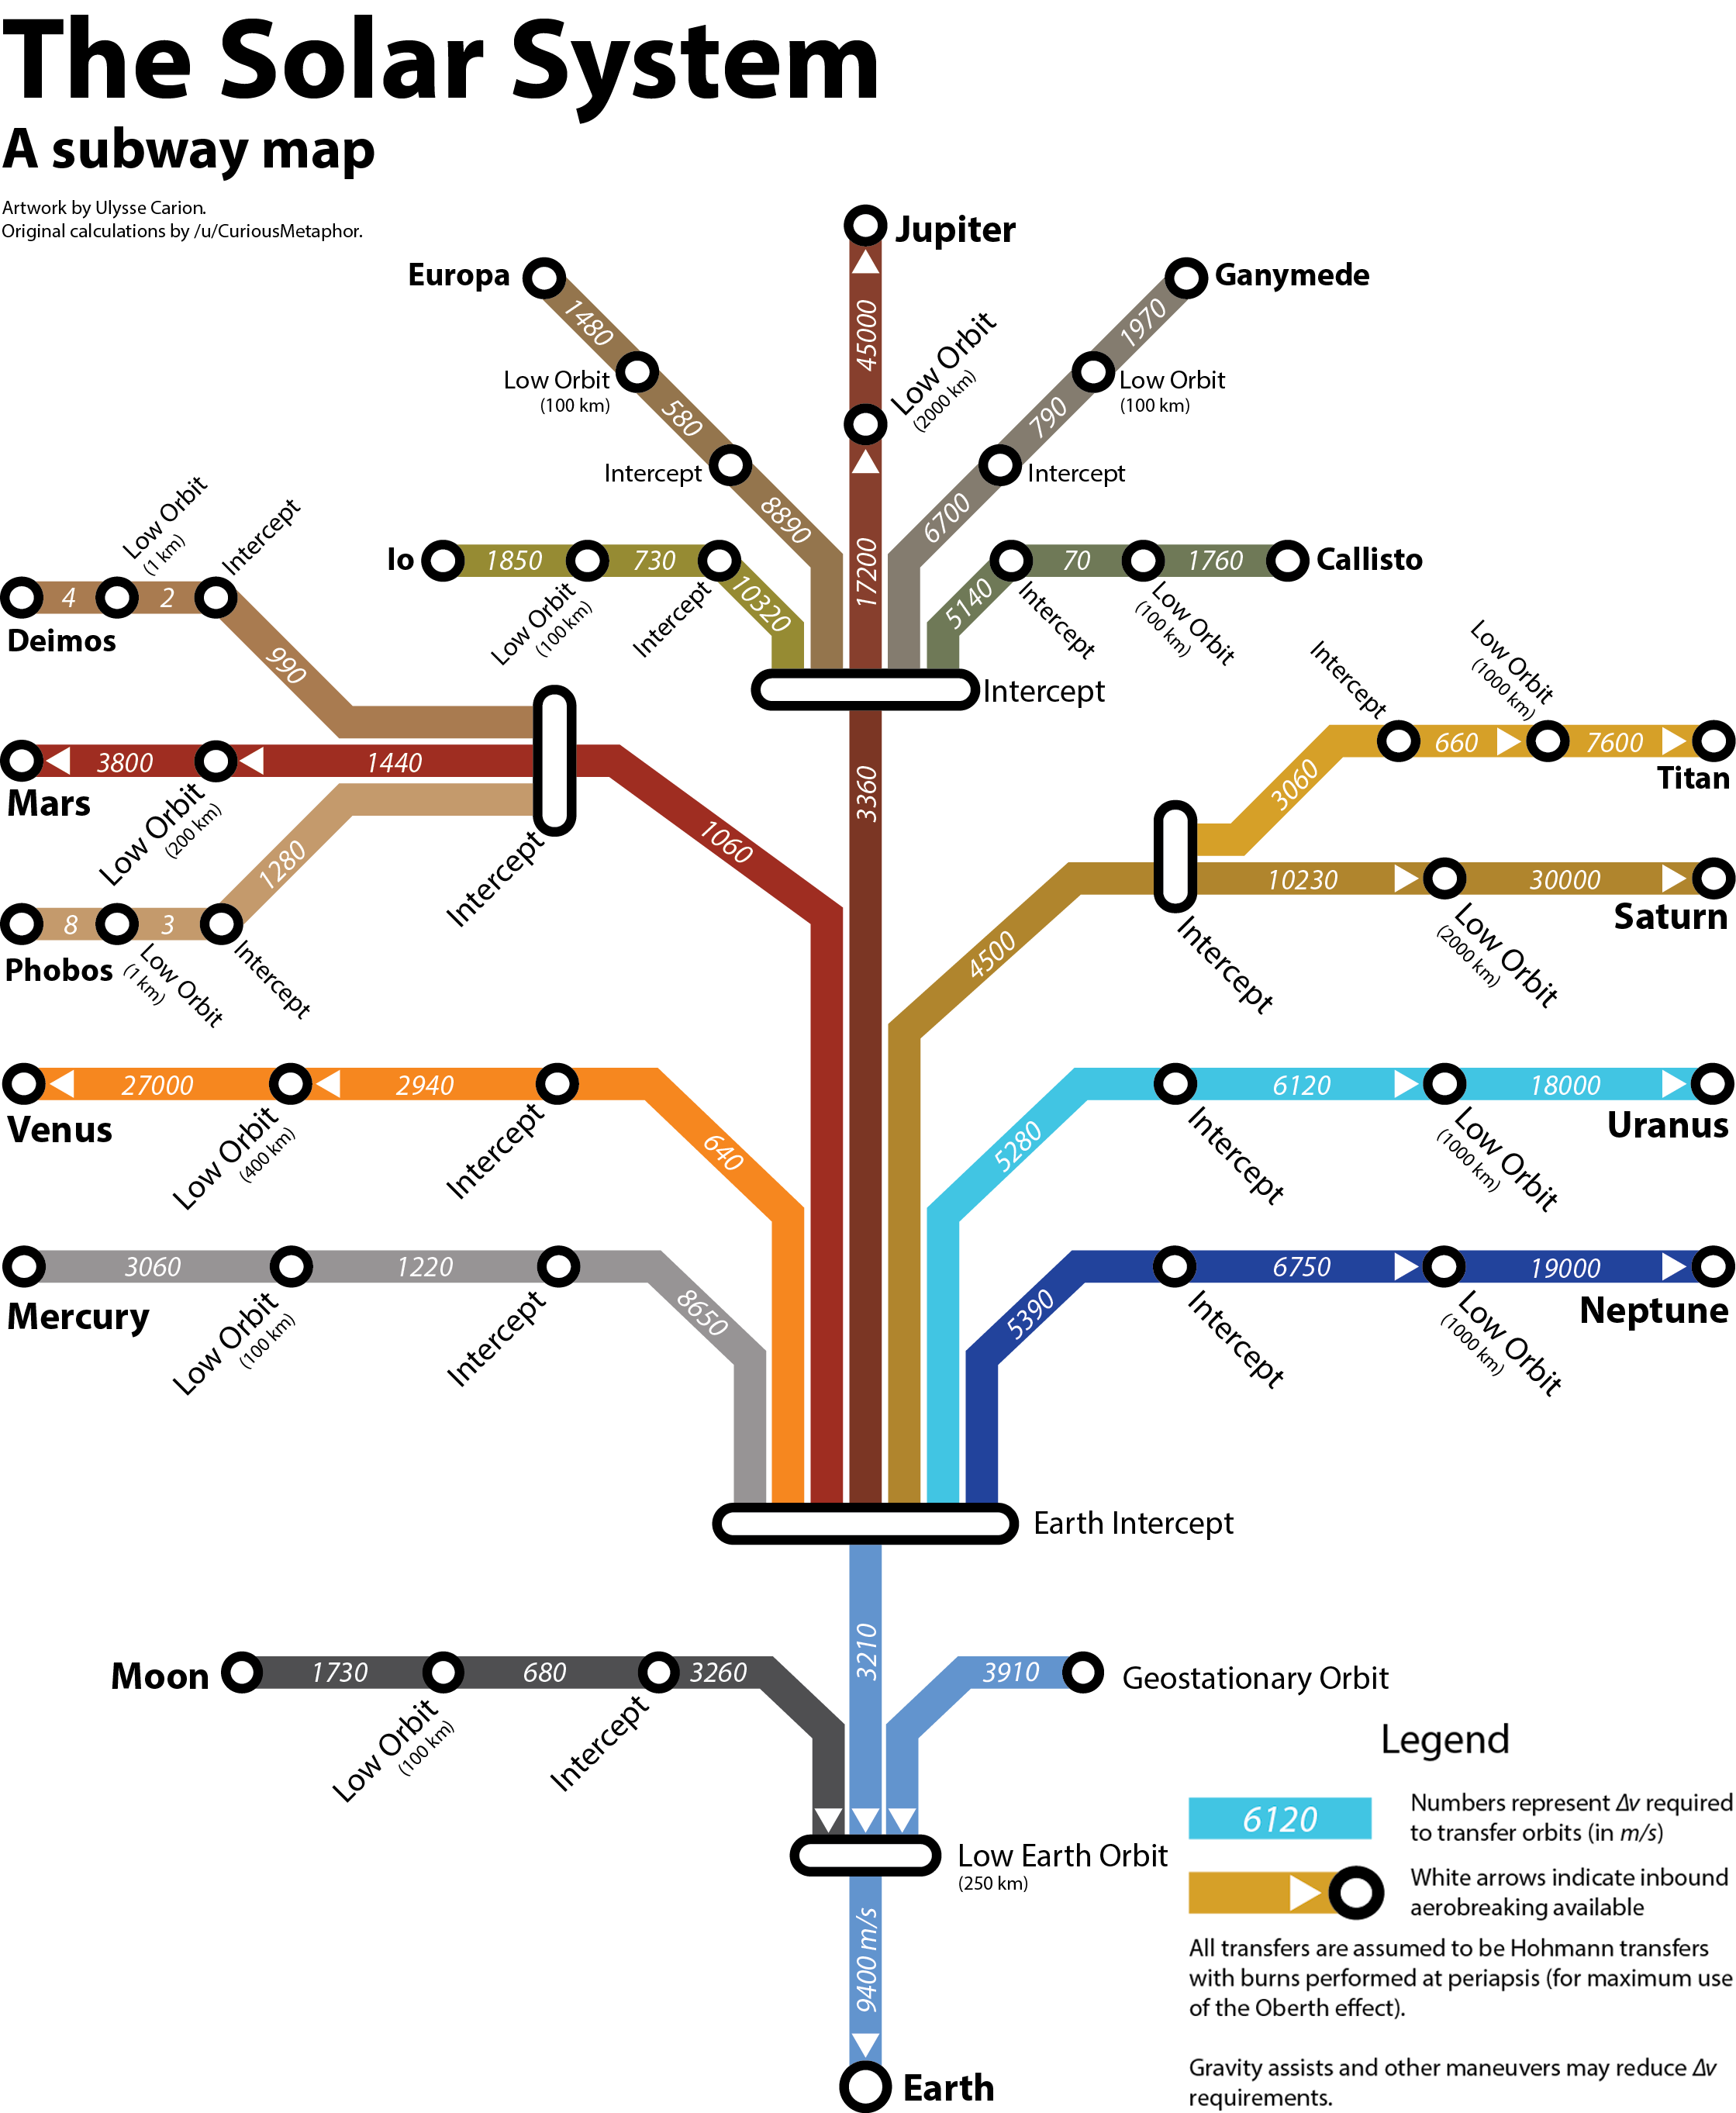
\includegraphics[width=\textwidth]{subway_map_legend}
  \caption{Representation of the different $\Delta V$ needed to go around the solar system, from \citet{reddit-subway}}
  \label{fig-subway_DV}
\end{figure}

\subsection{Rocket equation}
The thrust $T$ generated by ejecting mass at high velocity is
\begin{equation} \label{eq-thurst}
  T = v_{\rm ex} \dot{M}
\end{equation}
with $v_{\rm ex}$ the exhaust velocity of the propellant, and $\dot{M}$ the propellant mass flow rate through the thruster.
Hence,
\begin{equation} \label{eq-rocket}
  \Delta V = \int_{t_1}^{t_2} v_{\rm ex} \frac{ \norm{\dot{M}}}{M(t)} dt = v_{\rm ex} \ln \lp \frac{M_0}{M_1} \rp
\end{equation}
with $M_0 = M(t_0)$ and $M_1=M(t_1)$, and supposing that $v_{\rm ex}$ is constant.
We see from \cref{eq-rocket} that for a spacecraft of dry mass $M_1$ to have a given $\Delta V$, the exhaust velocity is directly linked to the initial \emph{wet} mass $M_0 = M_1 + M_{\rm prop}$, with $M_{\rm prop}$ the propellant mass.
\Cref{eq-rocket} is known as the (Tsiolkovsky) rocket equation.
Usually, instead of the exhaust velocity $v_{\rm ex}$, the specific impulse ${\Isp} = g_0 v_{\rm ex}$, with $g_0$ the standard gravity, is used.
\nomenclature[Q]{\ensuremath{ \Isp}}{ Specific impulse, related to the exhaust velocity of a propellant}
\nomenclature[P]{\ensuremath{ g_0}}{  Standard acceleration due to gravity \nomunit{9.80665 m/s$^2$}}

\subsection{Chemical space propulsion systems}
The usual rocket thruster uses a chemical reaction to generate the thrust.
For instance, the Vulcain (the thruster engine of the main stage of the European Ariane 5 and 6, developed by ArianeGroup, ex. Safran) uses the oxygen-hydrogen combustion, the most efficient chemical reaction \citep{nasa-H2O2}
\begin{equation*}
  2 {\rm H_2} + { \rm O_2} = 2 {\rm H_2 O} + 572 \text{~kJ},
\end{equation*}
with the energy of $572\,\kilo\joule$ of heat generated by $1\,\mole$ of oxygen.
This means that burning $1\,\kilo\gram$ of hydrogen-oxygen mixture generates a total energy of $13\,\mega\joule$. 
Supposing that the entire energy is converted into the exhaust of the water produced, its velocity would be of $5.1 \,\kms$.
In reality, the exhaust velocity of the Vulcain is of $4.2 \,\kms$, corresponding to $\Isp=431 \,\second$.
The efficiency of the Vulcain is close to 80\%, which is a very high efficiency, and it would be difficult to increase it significantly. 

In chemical propulsion systems, the fact that the energy released is related to the propellant mass gives an upper limit of exhaust velocity for a given combustion.
Electric propulsion engines, on the other hand, decouple the mass ejected (the propellant) from the energy source.
This decoupling allows a theoretical unlimited exhaust velocity.
Another advantage is the absence of reactive species, which lowers the security requirements impacting the spacecrafts.
Unfortunately, electric propulsion engines only work in vacuum and do not deliver sufficient thrust to compensate the earth gravity.
Hence, while electric propulsion can be used on spacecrafts, chemical propulsion is the only solution for rockets.

\subsection{Electric propulsion} \label{subsec-EP}
\ac{EP} systems mostly rely on plasmas \citep{charles2009,mazouffre2016}.
They have been successfully used since the 1960s by governments, but their complexity, the limited electric power available, and the inherent risk aversion of the space industry kept the \ac{EP} technologies hidden from the commercial applications \citep{lev2019}.
The breakthrough came in the '90s when the former Soviet Union's companies licensed the technology to western propulsion companies.
However, many commercial satellite manufacturers were skeptical, until the first decade of the 20th century, which brought strong evidence of the competitiveness of \ac{EP}.
The landmark of commercial use of \ac{EP} is the selling of four all-electric satellites for \ac{GEO} by Boeing in 2012, the first two of which were launched in March 2015.

The two leading \ac{EP} technologies used are
\begin{itemize}
  \item the \ac{HET}, also known as Stationary Plasma Thruster (SPT) in Russia
  \item the Gridded Ion Thruster (GIT), usually referred simply as Ion Thruster
\end{itemize}




 
 \paragraph{The Gridded Ion Thruster} is a plasma chamber closed at one end by two or more grids.
 The plasma source can be an emitting cathode, generating energetic electrons that ionize the propellant (usually Xenon), or a \ac{RF} source.
 The potential difference between the grids accelerates the ions.
 Another cathode is used to neutralize the ion beam.
 Compared to \ac{HET}s, it produces an ion beam with less divergence and a higher \Isp of the order of 3000 to 4000~s.
 \Cref{fig-iongridded} shows a picture of the ion thruster used for the BepiColombo mission toward Mercury.
 We see the neutralizing cathode, the accelerating grid, and the ion beam.
 
\begin{figure}[!hbt]
  \centering
  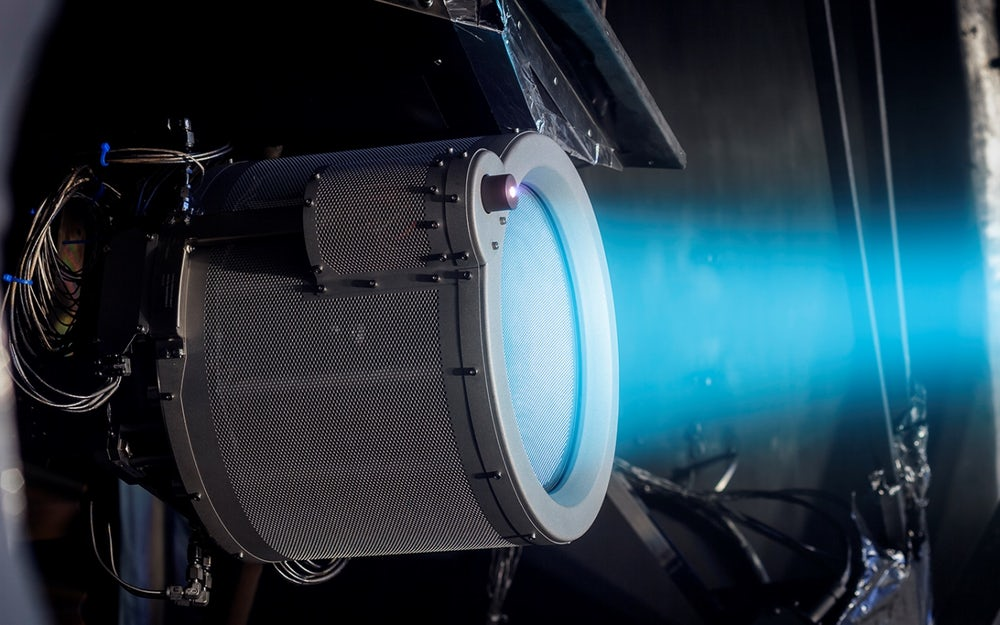
\includegraphics[width=\defaultwidth]{ion_Bepi}
  \caption{The T6 ion thruster will help send BepiColombo to Mercury. The neutralizing cathode is in the upper left quadrant of the thruster. (Credit\string: QinetiQ)}
  \label{fig-iongridded}
\end{figure}
 
 \paragraph{Hall Effect thrusters} use a magnetic barrier to both increase the ionization of the propellant and create the accelerating electric field.
 A detailed description of the \ac{HET} is presented in the next section.
 One cathode is used to start the discharge and neutralize the ion beam.
 Compared to GITs, \ac{HET}s need less power, hence reaching better thrust per power ratio and a smaller (therefore lighter) Power Processing Unit.
 Recently, the first satellites of two mega-constellations (OneWeb, 648 satellites planned, from which six were launched on February, the \nth{26} 2019, and Starlink, 12~000 satellites planned, from which 62 were launched on May, the \nth{23} 2019) were sent to Low Earth orbit, both using \ac{HET}s. 
 % Compared to GITs, \ac{HET}s need less power, and fewer power sources, hence reaching better thrust per power ratio and smaller (therefore lighter) Power Processing Unit. 
 Their typical \Isp is of the order of 1500~s.
 \Cref{fig-13kWHET} shows a high power prototype firing.
 We see the emitting cathode, in this design at the center, and the ion beam.
 \begin{figure}[!hbt]
   \centering
   \includegraphics[width=\defaultwidth]{HET_x3}
   \caption{A 13 kilowatt \acs{HET} prototype on a testing bench in a vacuum chamber (Credit\string: NASA).  }
   \label{fig-13kWHET}
 \end{figure}
 
 
 \subsection{EP environment in France} \label{subsec-HET_thruster}
 
 France is a leader country in the aerospace industry in both Europe and the world, with companies such as  Airbus, Thales, Safran, and ArianeGroup (join-venture of Safran and Airbus).
 As a consequence, the French ecosystem of electric propulsion is vibrant.
 The main thrusters produced in France are the PPS series by Safran, with the \PPS1350 (version G at 1.5~kW nominal power, and the version E at 2.7~kW), and the \PPS5000, a high power \ac{HET} at 5~kW, the first models of which have been delivered to Boeing in May 2019.
 A low-power version of the \PPS{}  is currently developed for low power, between 500\,W and 1\,kW\citep{vaudolon2018}.
 A list for the \PPS{} series elements and their respective characteristics can be seen in \cref{tab-ppsfamily}.
 \begin{table}[!hbt]
 \ra{1.3}
   \centering
   \caption{Members of the \PPS{} series developed by Safran Aircraft Engines \citep{boniface2017,duchemin2017,vaudolon2018}. The nominal operating condition of the \PPS{X00} is not fixed, yet.}
   \label{tab-ppsfamily}
   \begin{tabular}{@{}llll@{}} \toprule
   Name & Power & Thrust & \Isp \\ \midrule
   \PPS1350-G & 1.5~kW & 89~mN  & 1650~s \\
   \PPS1350-E & 2.7~kW & 140~mN  & 1800~s \\
   \PPS5000 & $3-5$~kW & $150-300$~mN  & $1850-1700$~s \\
   \PPS{X00} & $\sim 650$W &  $\sim$40~mN & $\sim 1450$~s \\
   \bottomrule
   \end{tabular}
 \end{table}
 
 Several initiatives concerning the small-sat sector are also undertaken, such as the start-ups Exotrail (micro \ac{HET}) and Thrust Me (radio frequency Ion Thruster), or the Electron Cyclotron Resonance Thruster at ONERA.
 Since 1996, numerous research projects have been carried out in France on HET with  the \ac{CNES}, SAFRAN and several research laboratories: ICARE, LAPLACE, CPHT, LPP, etc. \citep{boniface2017}.
 These numerous actors, combined with the support of the French and European space agencies, compose a stimulating environment that contributes both to the most mature technologies and the promising \ac{EP} concepts that could disrupt the propulsion sector.
 
% !TEX root=/home/tavant/these/manuscript/src/manuscript.tex

\section{Electric propulsion challenges}
\label{sec-challenges}
% \addcontentsline{toc}{section}{EP Industrial challenges}

Several challenges are currently tackled in the \ac{EP} industry.
The most prominent are listed by \citet{samukawa2012}\string:
\begin{enumerate}
  \item Performance improvement\string: efficiency, lifetime, and cost-effectiveness.
   Lifetime is an important issue and is limited by electrode or wall erosion.
   The lifetime of an electric thruster must be larger than 10 000 h of (reliable) operation.
   \item  Design of more versatile thrusters, i.e. able to operate at different combinations of thrust and propellant velocity.
   \item  Extension of the domain of operation to lower power ($\mu$N to 10 mN thrust range) for microsatellites or accurate attitude control.
   \item  Extension to higher power for orbit raising of telecommunication satellites (several tens of kW) and    interplanetary missions (100 kW and more).
   \item Extension of EP to low-altitude spacecraft\string: there is an increasing interest in civilian and military satellites flying  at altitudes around 100 km where the drag is significant and must be continuously compensated.
\end{enumerate}

\ac{HET} technology has the potential to answer many of these challenges.
For instance, the lifetime issue can be addressed with wall-less and magnetically shielded configurations.
Versatility is tackled with dual-mode \ac{HET} configuration \citep{boniface2017}, low power thruster is attained with $\mu$-thrusters \citep{lascombes2018}, and so forth.
However, the development of \ac{HET}s is slow and expensive. 
A better physical understanding of the processes governing \ac{HET}s is needed in order to reduce the cost and development times.
This is the objective of the current collaboration between Safran Aircraft Engines and \ac{LPP}.

% !TEX root=/home/tavant/these/manuscript/src/manuscript.tex


\section*{\acs{HET} research and development}
\label{sec-poseidon}
\addcontentsline{toc}{section}{\acs{HET} research and development}

Safran Aircraft Engines has been collaborating with \ac{LPP} since 2014, starting with the Ph.D. thesis of Viven Croes \citep{croes2017}.
During these first three years, a \ac{2D} \ac{PIC} code has been developed simulating the radial and azimuthal directions of a \ac{HET}.
Azimuthal instabilities have been observed in \citet{croes2017a}, and the effects of alternative propellants have been investigated in \citet{croes2018}.

From this fruitful collaboration, an ANR (Agence National de la Recherche) industrial chair {\sc Poseidon} for  "future Plasma thrusters for LOw earth orbit SatEllIte propulsiON systems", Grant No. ANR-16-CHIN-0003-01, has been created.
Its objective is to develop novel methods to reduce the development time and cost of the next \ac{EP} systems.
Both experiments and simulations are being developed to unlock the barriers of \ac{HET} development.
The {\sc Poseidon} chair is linked to the current development of a  low power \ac{HET} at Safran, the \PPS X00, which nominal operating point is of the order of 600W.
The scientific part of the chair is led by \ac{LPP}, while an unstructured \ac{3D} simulation code is developed by the CERFACS, in Toulouse.
Safran leads the technical development and experimental investigation.

At the beginning of my thesis, I participated in the development of a \ac{ML} of the \PPS X00.
The objectives of the \PPS X00-\ac{ML}  is to represent the physics of the \PPS X00 while allowing parametric studies of the main parameters of a \ac{HET}, such as the geometry, the magnetic field topology, or the wall material.
The \PPS X00-\ac{ML} has successfully shown its usefulness, as the first tests allow to obtain state of the art performances \citep{vaudolon2018}.
My work at Safran showed us that the development of \ac{HET} is still currently driven by experiments because numerical tools are not yet predictive.
Simulations can be helpful to engineers to obtain some insights for the thruster behavior, but cannot be used with confidence for development.
On the other hand, experiments are costly and time-consuming.
They also are prone to delays in the conception schedule, and reduce innovation as designers take fewer risks.

The lack of numerical tools comes from some physical phenomena that need to be better understood, even though \ac{HET} have been studied and used for more than 40 years.
% Hence a \emph{trial and errors} method is currently used by manufacturers for the development of the \ac{HET}.
These critical phenomena are \citep{samukawa2012,adamovich2017}
\begin{itemize}
  \item the electron transport,
  \item the plasma-surface interaction,
  \item the wall erosion,
  \item the propellant nature.
\end{itemize}

\vspace{1em}
The propellant nature impacts principally two things\string: the ion mass and the ionization energy.
Because of its high mass and low ionization energy, xenon has been used since the beginning of \ac{HET}. 
However, it is very costly, as it is mostly extracted from air with cryogenic distillation.
The atmosphere is composed in average of $\sn{9}{-6}\%$ of xenon \citep{earthfacs}.
The cheaper, but less effective, propellant of choice is krypton, which has recently started to be used.
Iodine could also be interesting, as it can be stored at room temperature in a solid state.
The impact of the propellant mass and chemistry is not yet clear and slows down the use of alternative propellants on already designed systems.

\vspace{1em}
The objectives of my thesis in the context of the {\sc Poseidon} chair focuses on the two first points -- the plasma wall interaction and the electron mobility -- and how they can influence each-other.
I also studied the wall erosion, but this work is classified, and will not be disclosed in this manuscript.






% !TEX root=/home/tavant/these/manuscript/src/manuscript.tex


\section*{Presentation of the Hall effect Thruster }
  \label{sec-HET}
  \addcontentsline{toc}{section}{Presentation of the Hall effect Thruster}

  
  The \ac{HET} is an electrostatic electrical propulsion system accelerating ions by the mean of an imposed voltage difference.
  \Cref{fig-bhtonoff} shows a picture of an \ac{HET} switched on and off.
  We can see the plasma in the annular plasma chamber.


  \begin{figure}[hbt]
    \centering
    \includegraphics[width=\defaultwidth]{PPS-ON_OFF.jpg}
    \caption{Front view off an \ac{HET}, the BHT-1500 from Busek, USA}
    \label{fig-bhtonoff}
  \end{figure}

  We can summarize the composition of an \ac{HET} with four parts\string:
  \begin{enumerate}
    \item The annular chamber.
    \item The injecting anode
    \item The cathode
    \item The magnetic circuit
  \end{enumerate}

  \begin{figure}[hbt]
    \centering
    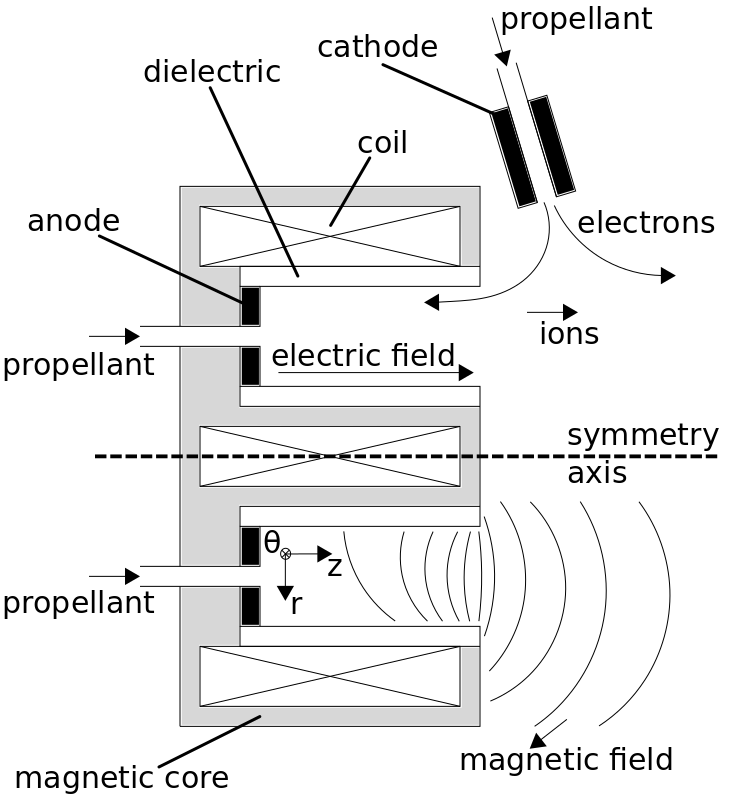
\includegraphics[width=\defaultwidth]{shematic_HET}
    \caption{Schematic cut of an \ac{HET}, illustrating its different parts. }
    \label{fig-shematiccut}
  \end{figure}

  \Cref{fig-shematiccut} presents a schematic cut of the \ac{HET} along its axial and radial direction.

  \paragraph{The chamber} has an annular shape.
  It is closed at the anode side and kept open at the other side.
  The axial length of the chamber is between $1$ and $3\,\centi\meter$; the radial width of the chamber is between $1$ and $2\,\centi\meter$. 
  The walls are usually constituted by a ceramic, as the \ac{BNSiO2}.
  The material needs to be resistant to erosion by ion impact sputtering.
  But changing the material is also known to affect the behavior of the discharge.
  The usually supposed phenomenon for this impact is the secondary electron emission yield that is a function of the material nature.
  For materials used in HET, this yield may be higher than one.


  \paragraph{The anode} is at the bottom of the chamber.
  The anode voltage is imposed to a few hundred volts.
  Usually, the neutral gas is injected through the anode itself, or close to the anode.
  The mass flow rate is of the order of a few mg/s.

  \paragraph{The cathode} is outside of the chamber.
  It is grounded, and injects electrons for two reasons\string:
  \begin{itemize}
    \item most of the electrons ($\sim 90 \%$) are used to neutralize the ion flux, for both allowing the ions to leave the thruster and avoiding charging of the spacecraft,
    \item  the others are attracted by the anode, hence entering the chamber. They enable the plasma discharge to switch and remain on.
  \end{itemize}

  \paragraph{The magnetic circuit} is composed of electromagnets and a magnetic circuit made of different ferromagnetic pieces.
  It creates a constant radial magnetic field in the annular chamber.
  The maximum value of the radial magnetic field is located close to the exit plane of the chamber.
  Its amplitude is on the order of $200$ Gauss ($\sn{2}{-2}$ T).

  \Cref{fig-bshape} illustrates the axial profile of the magnitude of the radial magnetic field.
  \begin{figure}[hbt]
    \centering
    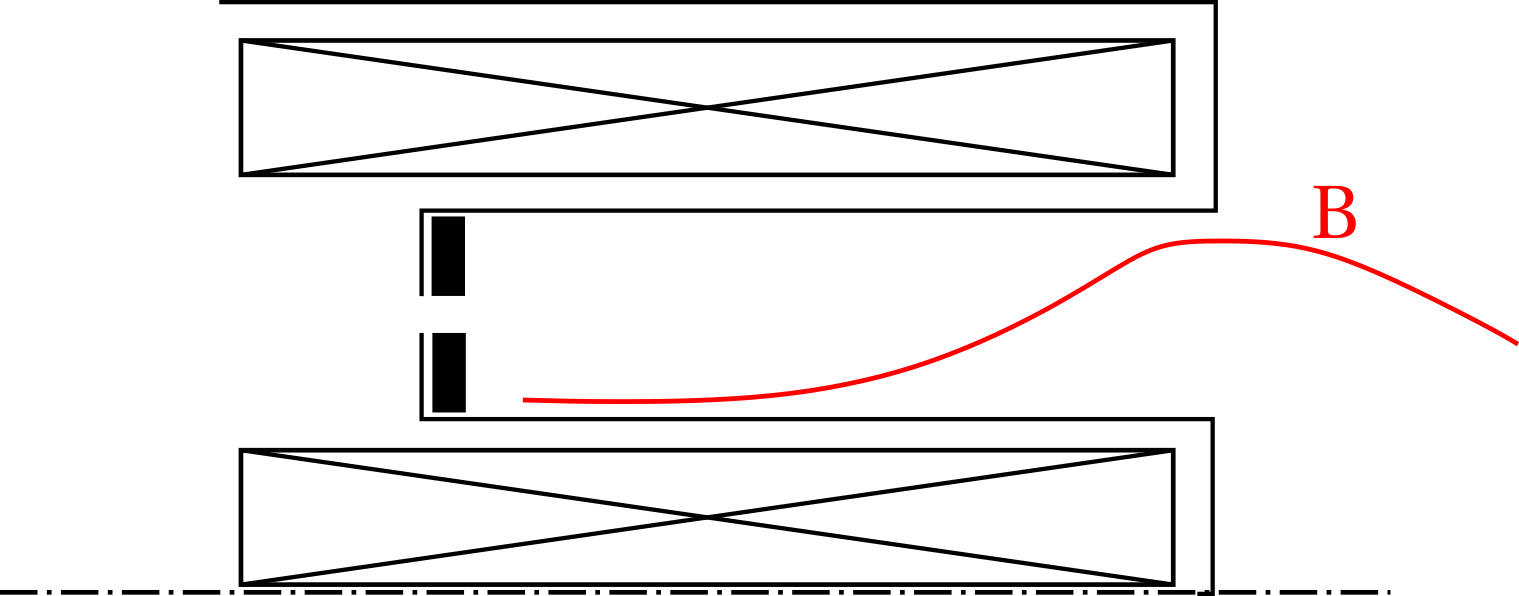
\includegraphics[width=\defaultwidth]{bshape}
    \caption{Usual shape of the axial profile of the radial magnetic field on the centerline of the channel.}
    \label{fig-bshape}
  \end{figure}


\section*{HET operating principle}
\addcontentsline{toc}{subsection}{HET operating principle}


  The operation principle of a \ac{HET} is rather simple.
  The objective is to ionize the propellant and impose an electric field to accelerate the ions.

  \paragraph{Ionization\\}
  The propellant, usually xenon, is ionized by electron-impact.
  The ionization energy needed is $\mathcal{E}_{\rm Xe, iz} = 12.13 \,\volt$, which corresponds to an electron velocity of $2000\,\kilo\meter\per\second$.
  Due to the low pressure (around $\sn{1}{-4}$ Pa), the mean free path of the electrons is larger than the chamber size.
  In consequence, a magnetic field is imposed in order to trap the electrons in a cyclotron motion.
  It increases the residence time of the electrons, thus promotes  ionization.
  In average in a well designed \ac{HET}, 90\% of the propellant is ionized.

  \paragraph{Acceleration\\}
  The potential difference  between the anode and the cathode is used to accelerate the ions outside of the chamber and create the thrust.
  Because the magnetic field slows the electrons down, the plasma resistivity increases in the region where the magnetic field amplitude is large.
  Hence, the axial profile of the magnitude of the axial electric field presents a maximum close to the maximum of the magnetic field.
  While the typical voltage difference is $U_d=300\,\volt$, the maximum electric field can be of the order of $30\,\kilo\volt\per\meter$ \citep{gawron2008}.

  \paragraph{Ionization and Acceleration regions overlap\\}
  \Cref{fig-zones} shows an illustration of the usual axial evolutions of the ionization and the electric and magnetic fields.
  As the magnetic field governs both the ionization and the acceleration regions, it can be challenging to obtain a clear separation between the two regions.
  However, if ionization happens in the acceleration region, the newly created ions will not be accelerated at their maximum velocity, hence resulting in a loss compared to the maximum theoretical thrust.
  The theoretical maximum speed is, by conservation of the total energy of the ion
  \begin{equation} \label{eq-vmaxtheo}
    v_{\rm ex, max} = \sqrt{ \frac{2 e V}{m_i} } \sim 31 \,\kilo\meter\per\second
  \end{equation}
  with $m_i = 131 \,\atomicmass$ for xenon and $V=300\,\volt$.


  \begin{figure}[hbt]
    \centering
    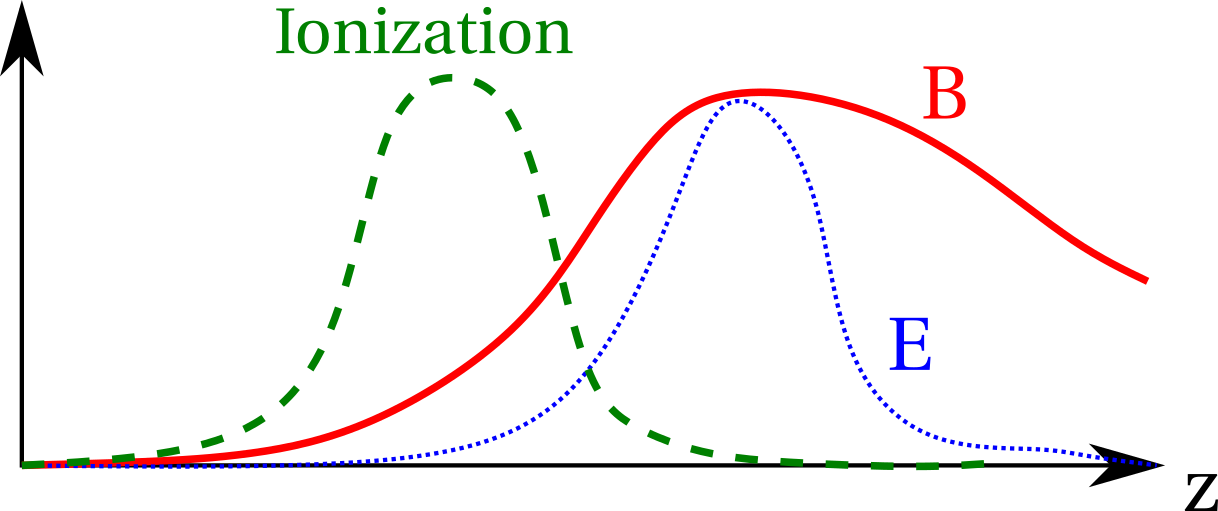
\includegraphics[width=\defaultwidth]{zones}
    \caption{Illustration of the usual axial profiles of the ionization and acceleration amplitude compared to the magnetic field.}
    \label{fig-zones}
  \end{figure}

  The thruster efficiency, in the usual configuration, is governed by its magnetic field topology.
  Hence, it can be tough to find the best topology that will optimize the ionization and the location of the ionization and acceleration regions.
  Some concepts of double stage \ac{HET} have been proposed to decouple the two phenomena to control them independently and are still under study \citep{dubois2018}.
  
  % However, the preliminary results are not as satisfactory as expected. 
  % \inlinenote{Add referecne here}
  % Moreover, the double-stage system needs more parts and power sources, resulting in a more complicated system.

  
  \section*{Instabilities present in the \ac{HET} }
  \label{sec-physics}
  \addcontentsline{toc}{subsection}{Instabilities present in the \ac{HET}}

  The \ac{HET}s are subject to numerous plasma oscillations, over a broad range of frequencies \citep{boeuf2017,choueiri2001}.
  The most important ones are\string:
  \begin{enumerate}
    \item Low frequency (10-20\,\kilo\hertz) ionization oscillations, usually referred to as breathing mode,
    \item Azimuthal low frequency rotating spokes, also in the \kilo\hertz{} range,
    \item Axial ion transit time oscillations, of the order of 100-500 \kilo\hertz,
    \item Azimuthal fast oscillations, of frequency of the order of the ion plasma frequency.
  \end{enumerate} 

  \paragraph{1. Breathing mode\\}
  The breathing mode is relatively well understood \citep{boeuf1998,barral2009,hara2014}.
  Indeed, a simple predator-prey model of two equations is enough to obtain the observed behaviour qualitatively.
  It is related to the idea that when the ionization is important, the neutral atom density decreases, reducing the ionization.
  Hence, the plasma density decreases, allowing the neutral density to rise again until the ionization grows up again.

  \paragraph{2. Rotating spokes\\}
  Experimental measurements with segmented anode \citep{ellison2012,mcdonald2011} seem to indicate that rotating spokes are present in the anode region.
  Their physical origins are less understood, as they were first attributed to ionization \citep{janes1966} but were later related to Simon-Hoh instability, and they were observed in \ac{PIC} simulations even with neglecting ionization \citep{carlsson2018}.
  However, in recent experiments, the presence of spokes did not seem to affect the \ac{HET} performances \citep{boeuf2018}.

  \paragraph{3. Transit time instability\\}
  Transit time instability has been predicted and observed in analytical and numerical models, respectively \citep{barral2005,boeuf2018}.
  Experimental studies of these instabilities are rather scarce, and it is only recently that time-resolved Laser-Induced Fluorescence measurements of the local ion velocity distribution function have confirmed the presence of this instability in a Hall thruster \citep{vaudolon2015}.
  This oscillation could reduce the performance of the thruster by increasing the overlap between the acceleration and ionization regions \citep{boeuf2018}.

  \paragraph{4. High-frequency azimuthal oscillations\\}
  These oscillations were first observed in \ac{PIC} simulations \citep{adam2004,ducrocq2006,adam2008a,heron2013} before being witnessed by electron Thomson scattering \citep{tsikata2009a,tsikata2009,tsikata2013}.
  They are essential, as they enhance the electron transport in the axial direction \citep{adam2004,lafleur2016a}.
  They are further described in the next section.

% !TEX root=/home/tavant/these/manuscript/src/manuscript.tex

\section*{Scientific challenges of the HETs}
\addcontentsline{toc}{section}{Scientific challenges of the HETs}

The scientific challenges are the critical phenomena not understood enough that prevent the industrial development of \ac{HET}s.
As introduced before, they concern the electron transport and the plasma-wall interaction.

\subsection*{Cross-field transport of the elections}
\addcontentsline{toc}{subsection}{Cross-field transport of the elections}

  \label{sec-mob}
  As a first approximation, the electrons are usually supposed frozen by the magnetic field.
  But in fact, they present a so-called cross-field transport toward the anode.
  For instance, because of collisions, the electrons can move from one magnetic line to another.
  This leads to a transport in the direction of the electric field.
  
  This transport can be expressed considering the electron momentum conservation equation \citep{lafleur2016a}\string:
  \begin{equation} \label{eq-elec_momentum_mobility}
    \partial_t(m_e n_e \vect{v}_{de}) + \grad \cdot (m_e n_e  \vect{v}_{de} \vect{v}_{de}) = q_e n_e ( \vect{E} + \vect{v}_{de} \times \vect{B}) - \grad \cdot \vect{\Pi}_e - m_e \nu_m n_e \vect{v}_{de},
  \end{equation}
  where $m_e, q_e$, $n_e$, $\vect{v}_{de}$, and $\vect{\Pi}_e $ are the electron mass, charge, density, drift velocity and pressure tensor, and $\nu_m$ is the electron-neutral momentum transfer collision frequency.
  Ignoring the electron inertia and the pressure term, and with $\vect{B} = B_0 \vect{e}_r$, we can write the conservation equation projected on the axial and azimuthal direction
  \begin{equation} \label{eq-elec_momentum_mobility2}
  \begin{cases}
    0 =  n_e E_z - n_e v_{de{\theta}} B_0 - \frac{m_e}{q_e} \nu_m n_e v_{dez}\\
    0 =  n_e E_{\theta} -  n_e v_{dez} B_0 - \frac{m_e}{q_e} \nu_m n_e v_{de{\theta}}
  \end{cases}
  \end{equation}
  Supposing that there is no electric field in the azimuthal direction ($E_{\theta}=0$),  we can combine the two equations of \cref{eq-elec_momentum_mobility2} and have \citep{chen2006,meezan2001}
  \begin{equation} \label{eq-mobility}
    \mobcla = \frac{n_e v_{dez}}{n_e E_z} = \frac{ \frac{\norm{q}}{m \nu_m}}{1 + \frac{\oce^2}{\nu_m}}
  \end{equation}
  with $\oce= \frac{\norm{q}B_0}{m}$ the cyclotron frequency.
  
  
  However, it has been observed in experiments by \citet{meezan2001} that the electron cross-field transport in the axial direction of the \ac{HET} is higher than $\mobcla$.
  Different phenomena have been proposed to explain the origin of this \emph{anomalous} transport.
  Two phenomena are supposed to be mainly responsible for this enhanced mobility \citep{croes2017}\string: the azimuthal instability and the near-wall mobility due to electron emission.
  A significant part of the work of this Ph.D. thesis concerns the quantitative comparison of the relative importance of the two phenomena.

  
  \subsection*{Electron drift and azimuthal instability in the HETs}
  \addcontentsline{toc}{subsection}{Electron drift and azimuthal instability in the HETs}

  The axial electric field $E$ and the radial magnetic field $B$ induces an azimuthal $E\times B$ drift of the electrons.
  The drift velocity $v_{\rm d, ExB}$ is 
  \begin{equation} \label{eq-exbdrift}
    v_{\rm d, ExB} = \bigg\lvert \frac{\vect{E} \times \vect{B}}{B^2} \bigg\rvert = \frac{E}{B} \sim \sn{1.5}{6} \,\meter\per\second
  \end{equation}
  Because of their large mass, the ions are not significantly affected by the magnetic field.
  Hence they do not drift azimuthally.
  As a consequence, there is a significant difference between the movement of electrons and ions in the azimuthal direction.

  This drift of electrons relative to the ions leads to instability in the azimuthal directions.
  Because the drift is perpendicular to the magnetic field, it is usually referred to as \ac{ECDI}.
  However, as it rises from an $E\times B$ drift, some authors use the name \ac{EDI}.
  In this thesis, we will use the name \ac{ECDI}.

  The actual nature of the \ac{ECDI} remains unclear\citep{boeuf2018}, as the \ac{ECDI} characteristics are very close to usual \ac{IAW}, and that experimental measurements are challenging to conduct in the range of parameter of interest.
  Hence, the community is still arguing about the actual nature of wave observed.
  A part of the work undertaken during my theses concerns the study and characterization of the instabilities observed in the kinetic simulations.
  These instabilities are treated in \cref{ch-5}.
  
\subsection*{Plasma-wall interaction}
\addcontentsline{toc}{subsection}{Plasma-wall interaction}

  The ceramic wall closes the chamber in the radial directions.
  It has been observed in experiments that the nature of the wall can significantly affect the discharge behavior \citep{gascon2003}.
  The primary phenomenon hold responsible for this observation is the electron emission.
  As usually observed in bounded plasmas, a floating sheath forms between the plasma and the dielectric wall.
  The sheath confines the electrons in the plasma and accelerates the ions toward the walls.
  This allows to obtain a flux of electrons equals to the flux of ions, resulting in charge conservation in the plasma, and a neutral flux, or also named zero-net current, to the surfaces.
  
  Due to the relatively high electron energy, the impact of a primary electron can lead to the emission of secondary electrons \citep{barral2003a,villemant2018}.
  The probability of \ac{SEE} depends on the electron impact characteristics (energy, angle) but also of the material\string: some materials are more emitting than others \citep{gascon2003}.
  Ion induced electron emission is much less likely to happen as the ions have a small impact energy.
  In addition to the near-wall conductivity discuss previously, these secondary electrons are accelerated toward the plasma by the sheath.
  Thus they modify the plasma and the sheath properties.
  Their impact on the electron temperature also affects the ionization rate, which is directly linked to the thruster efficiency.
  
  
  \citet{raitses2005} have observed that the current models of plasma-wall interactions with secondary electron emission cannot reproduce the electron temperature measured experimentally.
  The kinetic phenomena have been proposed by \citet{sydorenko2007} to explain this discrepancy between the models and the experiments.
  This could explain the differences between the kinetic simulations results and the global models in \citet{croes2017}.   
    
  \vspace{1em}
  In addition to \ac{SEE}, the ion impact energy is large enough to erode the walls by sputtering.
  This erosion is sufficient to be the main limitation of the lifetime of the \ac{HET}s.
  While most aspects of the erosion are well understood, we observe the apparition of  patterns with a typical scale of the order of the millimeter on the eroded surfaces.
  The origin and the possible implications of these erosion striations remain open questions.
  

\subsection*{Three-dimensional physics of the HET}
\label{sec-3Dphi}
\addcontentsline{toc}{subsection}{Three-dimensional physics of the HET}

The physics governing the \ac{HET} are three dimensional\string:
\begin{itemize}
  \item The plasma is accelerated in the axial direction by the electric field, and it is observed experimentally that the axial profile of the magnetic field is responsible for the performance of the thruster.
  \item The chamber walls close the radial dimension. The walls are responsible for most of the plasma losses, both on the particle and energy balances.
  \item The electrons drift in the azimuthal direction, leading to strong instabilities that affect the axial transport.
\end{itemize}

Consequently, when modeling or simulating a \ac{HET}, if one of the direction is not included, a part of the physics will be missing\string:
\begin{itemize}
  \item No axial direction\string: the ionization or the acceleration, as well as the plasma transport, are missing,
  \item No radial direction\string: the wall losses and interactions are missing,
  \item No azimuthal direction\string: the instability is missing. Hence the electron cross-field transport is not well represented.
\end{itemize}

While \ac{3D}-simulations have recently been proposed, they use scaling laws to simulate the system in a reasonable amount of time\citep{taccogna2019a}.
For instance, a reduced geometry is used in \citet{taccogna2018}, or a reduced density is used in \citet{fubiani2018a}.
A \ac{3D} simulation at real scale is not yet accessible.
Hence, we need to be able to rely on \ac{1D} or \ac{2D} simulations.
Consequently, we have to take into account the missing physics or include a model of its effects on the system.

% !TEX root=/home/tavant/these/manuscript/src/manuscript.tex


\section*{Plasma models and simulations}
\label{sec-simulations}
\addcontentsline{toc}{section}{Plasma models and simulations}

Depending on the pressure, energy, and time scale, different models are more adapted to describe the plasma.
There are mainly two distinct models.
The first is the \emph{kinetic} description of the species of the plasma, via the Boltzmann equation.
The second uses a \emph{fluid} description of the species, by means of moments.
% 
% \begin{figure}[hbtp]
%   \centering
%   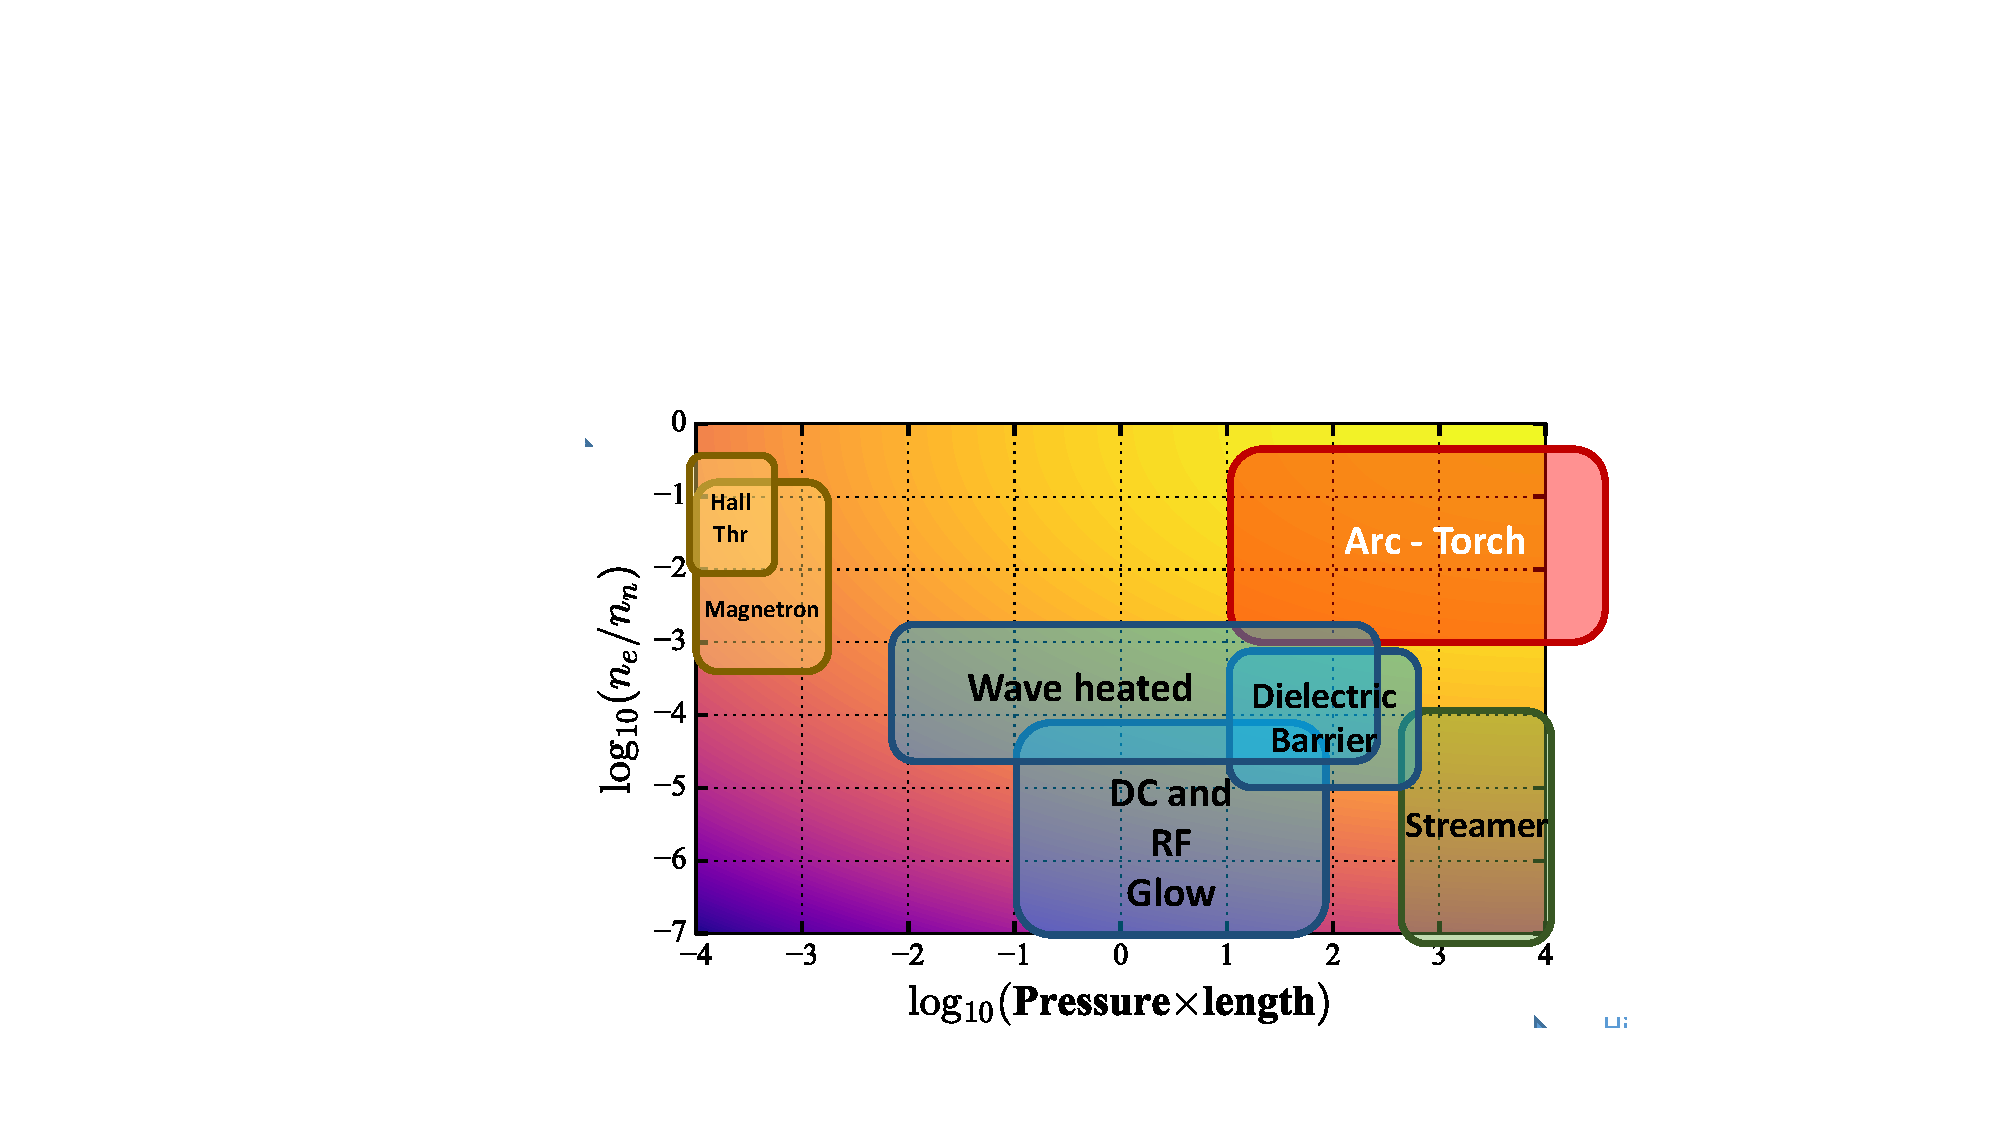
\includegraphics[width=\defaultwidth]{Chart}
%   \caption{}
%   \label{fig-chart}
% \end{figure}


\paragraph{Boltzmann equation \\}
The Boltzmann equation in \cref{eq-boltzmann} describes the evolution of the particles (atoms, ions and electrons) in the phase space.
The phase space is the set of each possible position $\vect{x}$ and velocity $\vect{v}$ that can be attained by a particle.
The evolutions in the phase space are due to forces, diffusion and collisions.

\begin{equation} \label{eq-boltzmann}
\deriv{f}{t}  + \vect{v} \cdot \grad_{\vect{x}} f + \vect{F} \cdot  \grad_{\vect{v}} f = \deriv{f}{t} \at{\rm coll}
\end{equation}
where $f$ is the distribution function of the particle at $\vect{x}, \vect{v}$, and $\deriv{f}{t}\mid_{\rm coll}$ denotes the effects of the collisions, $\grad$ is the gradient in both the positions (subscript $\vect{x}$) and the velocities (subscript $\vect{v}$)  and $\vect{F}$ is the force applied to the particle.
In the general electro-magnetic case,
\begin{equation*} \label{eq-forceEM}
  \vect{F} =  q \vect{E} + q \vect{v} \times \vect{B}
\end{equation*}
with $q$ the particle charge, $\vect{E}$ the electric field, and $\vect{B}$ the magnetic field.

\paragraph{Fluid equations \\}
The description on the plasma in 7 dimensions (3 of space, 3 of velocity, and one of time) can complicate the resolution of the Boltzmann equation.
If the precise description of $f$ is not needed, we can instead use the first moments of \Cref{eq-boltzmann} on the velocity in order to obtain a set of simpler equations.

The first equation is obtained by integrating \cref{eq-boltzmann} over the velocity space, which gives
\begin{align}
    & \iiint_{\vect{v}}  \deriv{f}{t} d^3v &&+&& \iiint_{\vect{v}}  \vect{v} \cdot \grad_{\vect{x}} f  d^3v &&+&&  \iiint_{\vect{v}}  \vect{F} \cdot  \grad_{\vect{v}} f  d^3v && = && \iiint_{\vect{v}}  \deriv{f}{t} \at{\rm coll} \nonumber  \\ 
   \iff &  \deriv{n}{t} &&+&&  \grad_{\vect{x}}  \cdot  ( \vect{u} n) &&+&& 0 &&=&& S_{\rm iz}   \label{eq-conc}
\end{align} 
where $n=\iiint f d^3v$ is the density, $\vect{u} = \frac{1}{n} \iiint \vect{v} f d^3v$ is the mean velocity, and $S_{\rm iz}$ is the source term of particle due to ionization.
\Cref{eq-conc} is the continuity equation for a given species.

In a similar fashion, integrating the Boltzmann equation times the velocity and the kinetic energy gives the momentum conservation equation and the energy conservation equation, respectively.
This set of equation is simpler to approach, although it relies on more hypotheses.

One of them is the closure of the system.
Indeed, the continuity equation describes the evolution of the density $n$ but needs the mean velocity $\vect{u}$.
However, the velocity is described by the momentum conservation equation that need the temperature $T$, and so on.
In order to close the system, one has to make a hypotheses on the higher moment of the distribution function.
A usual closure is the isothermal hypotheses, that fixes the temperature. 
Hence, the energy conservation equation is not needed.
Other closures possibles are the adiabatic hypotheses (no heath flux, the \nth{3} moment of $f$), the polytropic law linking the evolution of $n$ with $T$, or the Fourier law for heat diffusion.
% \inlinenote{Should we write the closes as equations ? $q = 0$, $T_e n_e ^{a}=cst$, etc. ?}


\subsection*{Plasma simulation models} \label{subsec-simulations}
As there are two different models to describe the plasma, there are two different simulation approaches \string: the fluid simulations and the kinetic simulations.
The fluid simulations solve the moments of the distribution function (the density, mean velocity and usually the temperature of the species), and the electromagnetic fields.
Depending of the conditions, the system of equation can be simplified before resolution.
In electrodynamic conditions, mainly for space plasmas and fusion, the Maxwell equations are coupled to the fluid equations leading to magnetohydrodynamics (MHD).
In the case of electrostatic conditions, as it is usual for Low Temperature plasmas, the Poisson equation is coupled to the fluid equations.
In most of low-temperature plasma, the plasma in quasi-neutral except in small regions as plasma sheaths close to walls.
It is also common to neglect inertia terms and assume a steady state in the momentum equations, leading to the drift-diffusion approximation
The fluid equations can be solved in \ac{3D}, \ac{2D} or \ac{1D} for space.
In low dimension model, the effects of the missing dimensions is usually added, for instance in the source terms as done by \citet{barral2003a}.


\vspace{1em}
However, some phenomena can only be described via the knowledge of the distribution function.
An example of such phenomena is the particle-wave interaction, as the Landau Damping \citep{landau1945,malmberg1964} or the plasma-beam instability \citep{filippychev1990}, for which the gradient of the distribution function in the velocity space is important.
In contrast to the fluid descriptions, \emph{kinetic} simulations solve the distribution function $f$ for both position and velocities.
Two approaches are usually used for kinetic simulations\string:
\begin{itemize}
  \item The \ac{DK} model, that discretize \Cref{eq-boltzmann} in the full phase space.
  \item The \ac{PIC} model, which uses an ensemble of particles to discretize the distribution function.
\end{itemize} 
While the \ac{DK} simulations use an Eulerian description of the distribution function, we can see the \ac{PIC} simulations as a Lagrangian approach.
The \ac{DK} simulations can theoretically better describe the plasma, mostly because there is less numerical noise and we can model binary collision more easily, especially Coulomb collisions.
On the other hand, \ac{PIC} simulations are much more simpler to develop on both a mathematical and a computation perspective.
For instance, the kinetic effect of electron emission have been recently studied using \ac{DK} simulation by \citet{cagas2019}, while it has been done since the last century in \ac{PIC} simulations \citep{boswell1988}.



% \input{Context/6_LPPic}
% !TEX root=/home/tavant/these/manuscript/src/manuscript.tex

\section{Problem statement and outline of the thesis}
\label{sec-problematic}
% \addcontentsline{toc}{section}{Problematic of the thesis}

My thesis takes part of the collaboration between Safran Aircraft Engines and the Laboratory of Plasma Physics, which objective is to study the fundamental physics governing the \ac{HET}, in the optic to accelerate the developments of the next generations of thrusters.
I mainly focused on the electron transport and the plasma-wall interaction,
both aspects requiring the use of kinetic tools.

Indeed, the electron transport is affected by instabilities that can only be described by kinetic models \citep{adam2008a,lafleur2016a}.
Furthermore, the plasma-wall interaction is also affected by kinetic effects, both concerning the electron emission induced by electron impact \citep{barral2003a,raitses2011,sydorenko2006} and the wall erosion by ion impact sputtering.
Relatively few simulation codes highly parallelized have been developed, that could allow parametric studies.
But the ever-increasing computational power available allows bigger simulations to be conducted.
Thus, a significant part of my work involves the development of a highly efficient \ac{PIC} simulation code, with all of the technical difficulties related to it.
The simulation code is then used to proceed to several parametric studies, that I used to derive reliable low-dimensional models that could be used to derive new engineering development tools.


\vspace{1em}
In \cref{ch-1}, we introduce \LPPic, the primary simulation model used in this work, with an emphasis on the axial convection of the particles and the plasma-wall interaction.
\cref{ch-5} focus on the azimuthal instability observed in the simulation and compares it to the dispersion relation.
\cref{ch-2} presents the results of a parametric study investigating the wall effect.
In \cref{ch-3,ch-4}, we modify the sheath model in order to reproduce the \ac{PIC} simulation results.
\cref{ch-3} focuses on a simplified \ac{1D} simulation to study the electron state law, while \cref{ch-4} continues the same model by including the secondary electron emission.
While the majority of the work studied the \ac{2D} radial and azimuthal simulation, we finish by study the radial direction in a \ac{2D} axial and azimuthal simulation in \cref{ch-6}.



% Remove the setting for the introduction
\let\leftmark=\oldleftmark
\let\rightmark=\oldrightmark

\renewcommand\thechapter\oldthechapter
\renewcommand\theHchapter\oldtheHchapter
\renewcommand\chaptername{Chapter}
% \acresetall

\let\leftmark=\oldleftmark
\let\rightmark=\oldrightmark

\renewcommand\thechapter\oldthechapter
\renewcommand\chaptername{Chapter}

% !TEX root=/home/tavant/these/manuscript/src/manuscript.tex

\chapter{Particle-In-Cell simulations of HETs}
\label{ch-1}
Structure :

{\bf Particle in Cell simulations} 20 pages
\begin{zzz}
  
  1.1 The HET
  1.2 Elements of the 2D PIC-MCC simulations

  1.3 Numerical implementation

  1.4 R-theta simulation: hypotheses
  
  1.5 focus on  Dielectrics : Poisson equation 

  1.6 Axial convection model
  
  1.7 Conclusion
\end{zzz}
\inlinenote{Is missing a part of the HET physics. Like the Boeuf Tutorial. }

The \ac{HET} has been studied since its first designs int he 1960's.
However, the physical processes the govern its behaviour stay ill-understood.
For most of them, as the electron cross field mobility or the plasma-surface interactions, kinetic informations are needed.


The next section present the basics of the \ac{PIC} - \ac{MCC} simulations, and the simulations code \LPPic that is develop at \ac{LPP}.


\inlinenote{add SEE models, discussions concerning the choice we did, a.s.o.}
 
% !TEX root=/home/tavant/these/manuscript/src/manuscript.tex


\subsection{The Hall effect Thruster }
\label{sec-HET}

The \ac{HET} is an electrostatic electrical propulsion system accelerating ions by the mean of an imposed voltage difference.
\Cref{fig-bhtonoff} shows a picture of an \ac{HET} switch on and off.
We can clearly see the plasma in the annular chamber.


\begin{figure}[hbtp]
  \centering
  \includegraphics[width=\defaultwidth]{PPS-ON_OFF.jpg}
  \caption{Front view off an \ac{HET}, the BHT-1500 from Busek, USA}
  \label{fig-bhtonoff}
\end{figure}

We can summarize the composition of an \ac{HET} with four parts:
\begin{enumerate}
  \item The annular chamber.
  \item The injecting anode
  \item The cathode
  \item The magnetic circuit
\end{enumerate}

\begin{figure}[hbtp]
  \centering
  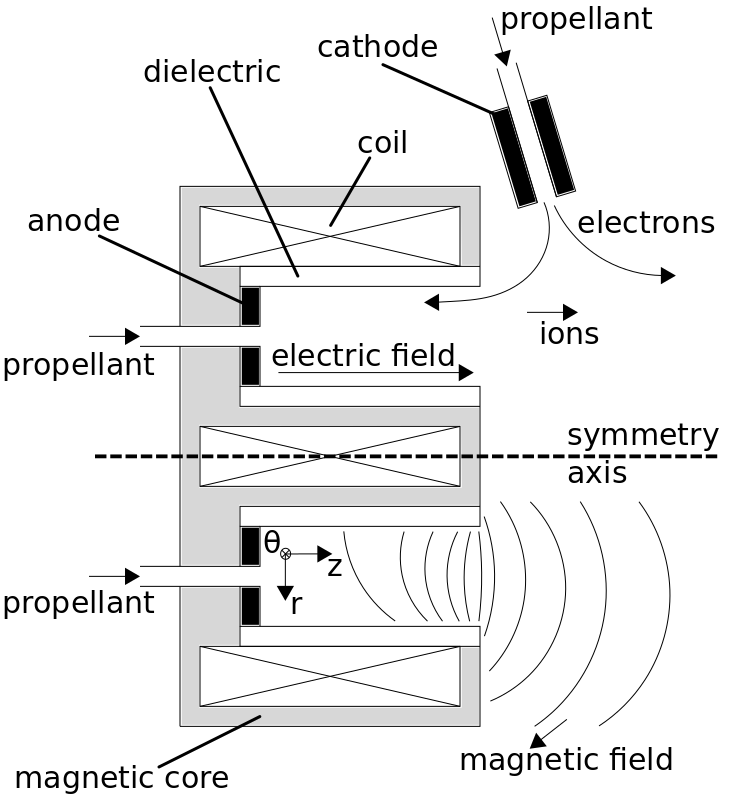
\includegraphics[width=\defaultwidth]{shematic_HET}
  \caption{Schematic cut of an \ac{HET}, illustrating its different parts. }
  \label{fig-shematiccut}
\end{figure}

\Cref{fig-shematiccut} presents a schematic cut of the \ac{HET} along its axial and radial direction.

\paragraph{The chamber} has an annular shape.
It is open closed at the anode side, and kept open at the other side.
The walls are usually constituted by a ceramic, usually \ac{BNSiO2}.
The material needs to be resistant to erosion by ion impact sputtering.
But changing the material is also known to affects the discharge behaviour.
The usually supposed phenomena for this impact is the secondary electron emission yield that is a function of the material nature.


\paragraph{The anode} is at the bottom of the chamber.
The anode voltage is imposed to a few hundred volts.
Usually, the neutral gas injection is made by the anode itself for
The mass flow rate is of the order of a flew mg/s.

\paragraph{The cathode} is outside of the chamber.
It is grounded, and injects electrons for two reasons:
\begin{itemize}
  \item most of the electrons ($\sim 90 \%$) are used to neutralize the ion flux, for both allowing the ions to leave the thruster and avoid charging of the spacecraft.
  \item some of the electrons are attracted by the anode, hence entering the chamber and allowing the plasma discharge and switch and remain on.
\end{itemize}

\paragraph{The magnetic circuit} is composed of electromagnets and a magnetic circuit mode of ferromagnetic material.
It create a constant radial magnetic field in the annular chamber.
The maximum value of the radial magnetic field is located close to the exit plan of the chamber.
Its amplitude is on the order of $200$ Gauss ($\sn{2}{-2}$ T).

\Cref{fig-bshape} illustrate the axial profile of the amplitude of the radial magnetic field.
\begin{figure}[hbtp]
  \centering
  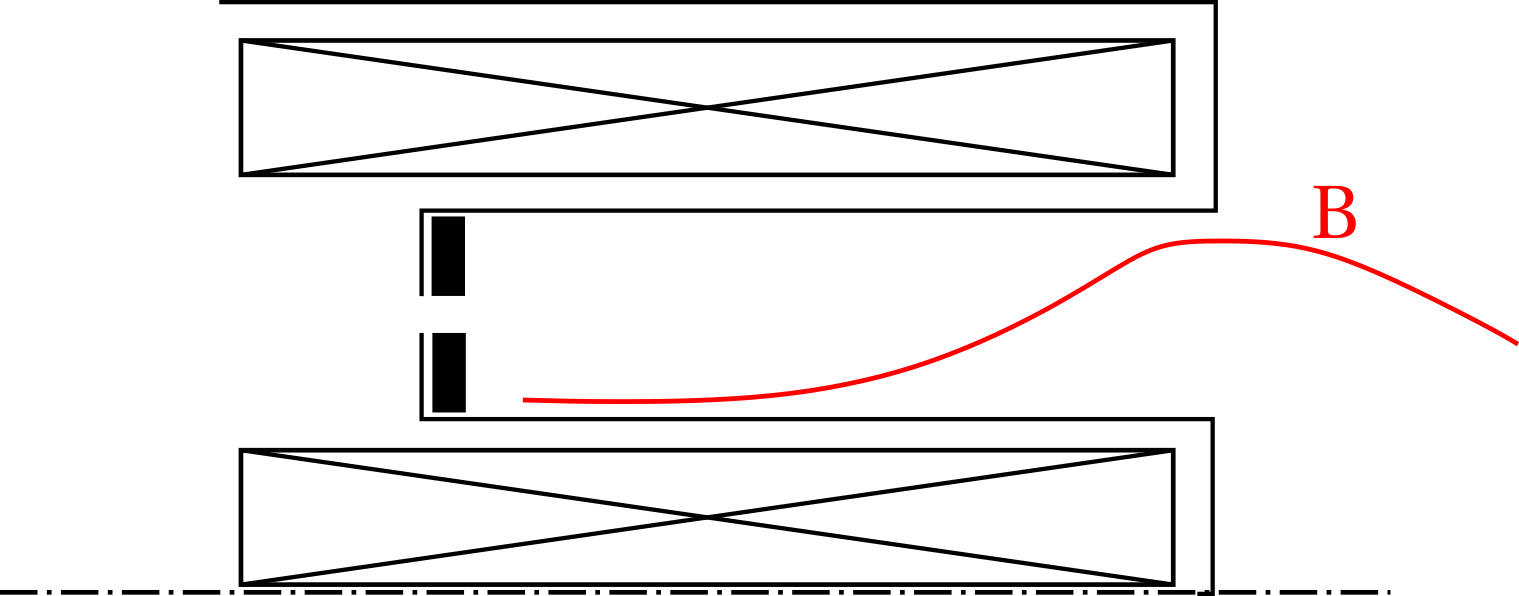
\includegraphics[width=\defaultwidth]{bshape}
  \caption{Usual shape of the axial profile of the radial magnetic field on the centreline of the channel.}
  \label{fig-bshape}
\end{figure}


\subsection{Operating principle}

The operation principle of an \ac{HET} is rather simple.
The objective is to ionize the propellant and impose an electric field to accelerate the ions.

\paragraph{Ionization}
Due to the low pressure (around $\sn{1}{-4}$ Pa), the mean free path of the electrons is too large, compared to the chamber size.
In consequence, we impose the magnetic field in order to trap the electrons in a cyclotron motion, increasing the residence time of the electron, and the ionization.
In average, 90\% of the propellant is ionized in an well designed \ac{HET}.

\paragraph{Acceleration}
The potential difference  between the anode and the cathode is used to accelerate the ions outside of the chamber and create the thrust.
Because the magnetic field slows the electrons down, the plasma resistivity increases in the region where the magnetic field amplitude is large.
Hence, the axial profile of the amplitude of the axial electric field presents a maximum close to the maximum of the magnetic field.

\paragraph{Ionization and Acceleration regions overlay}
As both the ionization region and the acceleration region are governed by the magnetic field, it can be difficult to obtain a net separation.
However, if ionization append in the acceleration region, the newly created ions will not be accelerated at their maximum velocity, hence resulting in a loss compared to the maximum theoretical thrust.

\Cref{fig-zones} shows an illustration of the amplitude of the ionization and the acceleration due tot he electric field.
\begin{figure}[hbtp]
  \centering
  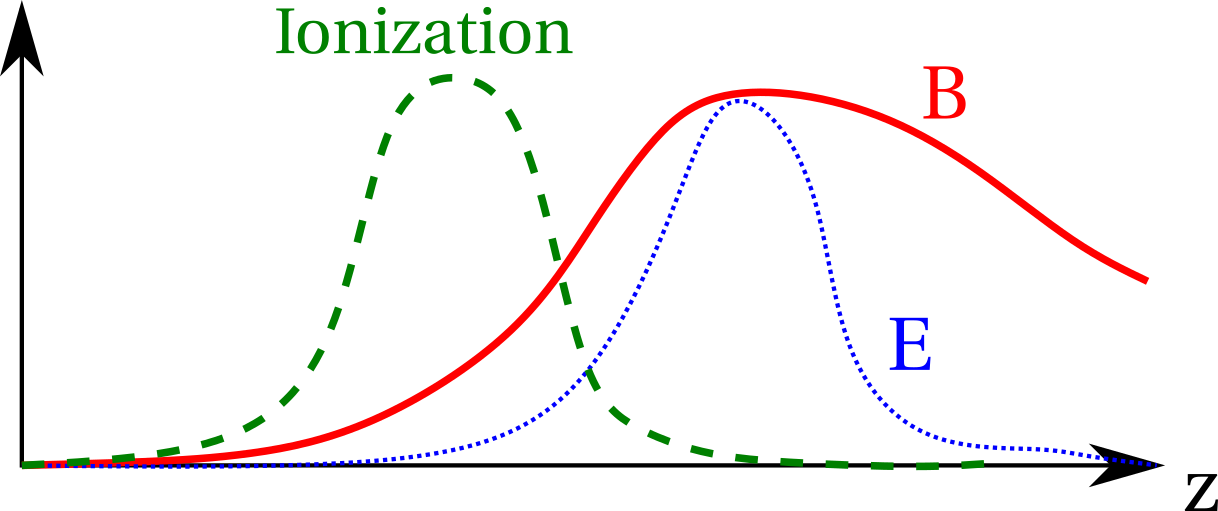
\includegraphics[width=\defaultwidth]{zones}
  \caption{Illustration of the usual axial profiles of the ionization and acceleration amplitude compared to the magnetic field.}
  \label{fig-zones}
\end{figure}

The thruster efficiency, in the usual configuration, is governed by its magnetic field topology.
Hence, it can be difficult to find the best topology that will optimize the ionization and the location of the regions.

Some concepts of double stage \ac{HET} have been proposed to decouple the two phenomena in order to control them independently.
However, the preliminary results are not as satisfactory as expected.
Moreover, the double-stage system needs more parts and power sources, resulting in a more complicated system.
Hence, we keep studying the usual single-stage configuration.

\subsection{Electron Drift and azimuthal instability}
The axial electric field $E$ and the radial magnetic field $B$ induces an azimuthal $E\times B$ drift of the electrons.
Because the ions are not significantly affected by the magnetic field, they do not drift.

As a consequence, they is a strong drift of the electron in respect  to the ions.
This drift can lead to instability in the azimuthal directions.
Because the drift is perpendicular to the magnetic field, it is usually called \ac{ECDI}.
However, as it rises from an $E\times B$ drift, some authors uses the name \ac{EDI}.

Azimuthal oscillations have been observed both experimentally and in simulations.
However, as the \ac{ECDI} characteristic are very close to usual \ac{IAW}, the community is still arguing about the actual kind of wave observed.


\subsection{Plasma-wall interaction}
The ceramic wall closes the chamber in the radial directions.
As usually observed in bounded plasmas, a floating plasmas sheath forms between the plasma and the dielectric wall.
The sheath confines the electrons in the plasma and accelerates the ions toward the walls.
This allows to obtain a flux of electron equals to the flux of ion, resulting in a charge conservation in the plasma, and a neutral flux, also named zero-net current to the surfaces.

Due to the relatively high electron energy, the material can emit electrons induced by electron impact.
These secondary electrons are accelerated toward the plasma, and so modify the plasma and the sheath properties.
The probability of \ac{SEE} depends of the electron impact characteristics (energy, angle) but also of the material: some material are more emitting than others.


\subsection{Cross field transport of the elections}
The electrons are not only drifting in the azimuthal directions.
For instance, because of collisions, the electrons can move from one magnetic line to another.
This leads to a cross-field transport in the direction of the electric field.

It has been observed in \ac{HET} that the electron cross-field transport is higher than the one only due to collisions.
Recently, the \ac{ECDI} has been proposed to induce this so-called anomalous transport of the electrons.

Another phenomena that can leads to increased cross-field transport in the \ac{NWC}.
It is due to electron collisions with the wall, inducing \ac{SEE}.


\section{Three-dimensional physics}
\label{sec-3Dphi}

The physics of the \ac{HET} is really three dimensional:

\begin{itemize}
  \item The plasma is accelerated in the axial direction. The axial profile of the magnetic field is responsible for the performance of the thruster.
  \item The radial dimension is closed by the chamber walls. The walls are responsible for most of the plasma losses, both on the particle and energy balances.
  \item The electrons drifts in the azimuthal direction, leading to instabilities.
\end{itemize}

Consequently, when simulating an \ac{HET}, if one of the direction is not model, a part of the physics will be missing:
\begin{itemize}
  \item Missing axial direction: the ionization and the convection are missing
  \item Missing radial direction: the wall losses and interactions are missing
  \item Missing azimuthal direction: the \ac{ECDI} is missing, hence the electron cross-field transport is not well represented.
\end{itemize}

While 3D-simulations have recently been proposed, they uses scaling laws to simulate the system in a reasonable amount of time.
A simulation at scale {1:1} is not yet accessible.
Hence, we need to rely on \ac{1D} or \ac{2D} simulations.
Consequently, we need to take into account the missing physics or include a model of its effects on the system.

% !TEX root=/home/tavant/these/manuscript/src/manuscript.tex

\section{Elements of the 2D PIC-MCC simulations}
  \label{sec-elements}
  \subsection{Principe of the PIC simulations}

    The \ac{PIC} simulation models particles moving freely on a grid.
    The grid is used to compute the electric field, in the electrostatic approximation by solving the Poisson equation

    \begin{equation}
      \label{eq-poisson}
      \Delta \phi = - \frac{\rho}{\epsilon_0}
    \end{equation}

    where $\phi$ is the electric potential, $\rho$ is the charge density, and $\epsilon_0$ the vacuum permittivity.
    If the electrostatic approximation is not correct, one needs to solve the Maxwell equations.

    The particles move following the Lorenz forces
    \begin{equation}
      \label{eq-Lor}
      m \vec{a} = q \vect{E} + q \vec{v} \times \vec{B}
    \end{equation}
    with $m$ and $q$, the particle mass and electric charge, respectively.
    The numerical particles followed in the simulations correspond to $q_f$ physical particles, with
    \begin{equation}
      q_f = \frac{n V}{\Npc}
    \end{equation}
    with $n$ the particle density, $V$ the volume of a cell, and $\Npc$ the number of numerical particles in a cell.
    A large enough number of particles is needed in order to obtain physical results.
    Indeed, an insufficient number of particles leads to numerical heating \cite{ueda1994}.
    Usually, a minimum of 100 particles per cell are used, but recent results seem to encourage to use more particles \cite{janhunen2018}.

  \subsection{Monte Carlo collisions}

    In \ac{PIC} simulations, collisions between charged and neutral particles can be modeled by binary collision, but this approach is computationally costly.
    Instead, a Monte-Carlo algorithm can be used \cite{vahedi1995}.
    This approach is very efficient and allows scattering, momentum transfer, and ionization to be consistently modeled.
    The propellant used in \ac{HET} is \ac{Xe}.
    The cross-sections used for modeling \ac{Xe} or other gases collisions are taken from the {\sc LXCat} database project \cite{LXCat_web,pancheshnyi2012}.
    Except if otherwise stated, the elastic, inelastic scattering and ionization reactions listed in \cref{tab-reactXe} are used.
    The cross-section values are summarised in \cref{fig-xexsection}.

    \begin{table}[hbtp]
      \ra{1.3}
      \centering
      \caption{Reactions for xenon used in the PIC simulations}
      \label{tab-reactXe}
      \begin{tabular}{@{}lll@{}}  \toprule
        Reaction & Threshold & Reference\\ \midrule
        {\it Elastic scattering} & &\\
        e + Xe = e + Xe   & --   & \cite{Lxcat_Xe,Lxcat_Xe2} \\
        {\it Excitation} & &\\
        e + Xe = e + Xe$^*$   & 8.315eV   & \cite{Lxcat_Xe,Lxcat_Xe2} \\
        e + Xe = e + Xe$^*$   & 9.447eV   & \cite{Lxcat_Xe,Lxcat_Xe2} \\
        e + Xe = e + Xe$^*$   & 9.917eV   & \cite{Lxcat_Xe,Lxcat_Xe2} \\
        e + Xe = e + Xe$^*$   & 11.7eV    & \cite{Lxcat_Xe,Lxcat_Xe2} \\
        {\it Ionization} & &\\
        e + Xe = e + Xe$^+$   & 12.13eV   & \cite{Lxcat_Xe,Lxcat_Xe2} \\
        \bottomrule
      \end{tabular}
    \end{table}



    \begin{figure}[hbtp]
      \centering
      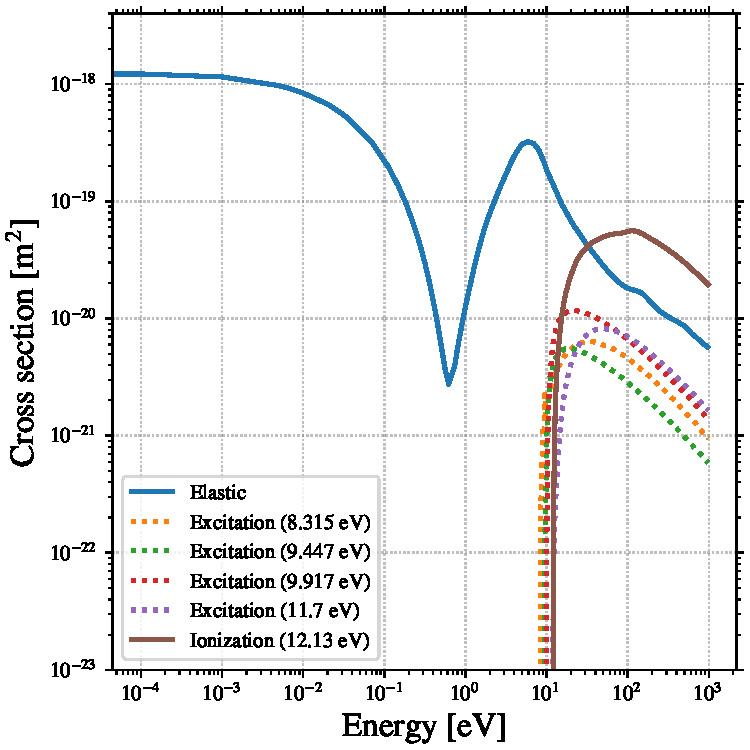
\includegraphics[width=\defaultwidth]{figure/xenon_cross_section.pdf}
      \caption{Cross section values used in the Monte Carlo procedure \cite{Lxcat_Xe,Lxcat_Xe2}.}
      \label{fig-xexsection}
    \end{figure}


\section{Numerical implementation of the Particle in cell simulation}

  \LPPic is an explicit electrostatic \ac{PIC}-\ac{MCC} simulation code.
  Every time-step, the simulation loop presented in \cref{fig-picloop} is computed.
  The different steps constituting the PIC-loop are described in the next subsections.
  \begin{figure}[hbtp]
    \centering
    \smartdiagramset{circular distance=4.5cm,
    module minimum width=3.5cm,
    text width=3cm,
    arrow tip=to}
    \smartdiagram[circular diagram:clockwise]{Particle Motion ,Boundary,Collision,Density weighting, Poisson Equation, Field weighting}
    \caption{\ac{PIC}-\ac{MCC} loop executed every time step.}
    \label{fig-picloop}
  \end{figure}


  \subsection{Data used}
    In \ac{PIC} simulations, there are two kinds of data used\string:
    \begin{itemize}
      \item Particles (electrons, ions, neutrals can be followed as well but not in \LPPic)
      \item Mesh, also named fields (densities, electric and magnetic fields, and so on)
    \end{itemize}

    \paragraph{Particles\\}
    For each particle, are known its position $\vec{x}$ and its velocity $\vec{v}$.
    In most \ac{PIC}-\ac{MCC} simulations, the three directions of the velocity vector are followed in order to take into account scattering.
    It is abbreviated as \acs{3V}.
    The particle positions and velocity are not discretized, except to the numerical floating-point precision.

    \paragraph{Fields\\}
    The fields are defined at the center of each cell of the mesh.
    The charge density $\rho$ is computed by depositing the particle on the mesh, using the Cloud-in-cell model \cite{birdsall1991}.
    The electric field at the position of the particle is also obtained by bilinear interpolation.
    The mesh dimension defines the dimension of the simulation.
    It is usual to find \acs{1D}\acs{3V} or \acs{2D}\acs{3V} \ac{PIC} simulations, for particles with 3 directions on the velocity but one (or two) dimensions in space.

    \subsection{Particle pusher}
    The interaction of the movement equation \cref{eq-Lor} is different for magnetized and non-magnetized particles.
    For non-magnetized particles, we use the leapfrog scheme \cite{birdsall1991}
    \begin{align}\label{eq-leapfrog}
      \vect{v}^t &= \vect{v}^{t-1} + \frac{q}{m} \vect{E} \dt, \\
      \vect{x}^t &= \vect{x}^{t-1} + \vect{v}^t \dt,
    \end{align}
    with the superscript $t$ designing the time step, $q$ and $m$ the particle electric charge and mass, $\vect{E}$ the electric field at the particle position, and \dt the time step duration.

    It is important to note that the leapfrog induces a shift of $\frac{\dt}{2}$ between the position and the velocity, as illustrated in \cref{fig-leapfrog}.
    \begin{figure}[hbtp]
      \centering
      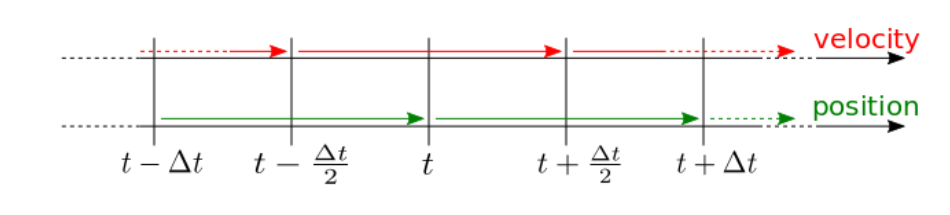
\includegraphics[width=\defaultwidth]{leapfrog.png}
      \caption{Illustration of the shift between the particle velocity and position.}
      \label{fig-leapfrog}
    \end{figure}
    This shift can lead to erroneous diagnostics when computing moments of the particles distribution.
    For instance, the mean velocity of an ensemble of $N$ particles at the instant $t$ is computed as\string:
    \begin{equation} \label{eq-meanv}
      \mean{\vect{v}}^t = \frac{1}{N} \sum_i^N \lp \vect{v_i}^t + \frac{q}{m} \vect{E_i} \frac{\dt}{2} \rp.
    \end{equation}
    Other moments like the mean energy or heat flux follow the same correction.
    We can see that the error between $\mean{\vect{v}}$ defined above and
    $$ \tilde{\vect{v}} = \frac{1}{N} \sum_i^N  \vect{v_i}^t $$
    is
    $$ \mean{\vect{v}} - \tilde{\vect{v}} =\frac{q \dt}{2 m}  \frac{1}{N}  \sum_i^N  \vect{E_i} .$$
    Hence, the error in the diagnostic is larger in the region of large electric field (as in the sheaths).

    \paragraph{Magnetized particles}
    For magnetized particles, we use a modification of the leapfrog algorithm proposed by Boris \cite{boris1970}.
    It corresponds to an operator splitting between the electrostatic acceleration and the magnetic rotation.
    This splitting is described below\string:

    \begin{enumerate}
      \item accelerate the particle during $\frac{\dt}{2}$\string: $\vect{v}^{t-\frac{\dt}{2}} = \vect{v}^{t-1} + \frac{q}{m} \vect{E} \frac{\dt}{2}$
      \item rotate the particle velocity with the magnetic field
      \item accelerate the particle during $\frac{\dt}{2}$\string: $\vect{v}^t = \vect{v}^{t-\frac{\dt}{2}} + \frac{q}{m} \vect{E} \frac{\dt}{2}$
    \end{enumerate}


  \subsection{Poisson equation solver}
  \label{subsec-poissonintro}

    In order to compute the electric field due to the particle charge density, the Poisson equation \cref{eq-poisson}  needs to be discretized over the mesh.
    We can directly discretize the differential operator by using the finite volume approach over a cell of the mesh.
    The formal discretization is developed in \cref{sec-diel}, for the particular case of taking into account the presence of dielectric boundaries.

    In \ac{1D}, the obtained linear system is tridiagonal.
    It can be solved directly using {\sc Thomas}' algorithm, which stores the Gauss elimination's coefficient.
    In \ac{2D}, the linear system is pentadiagonal.
    A direct solver, like the $LU$ decomposition, would require a large amount of memory to store the factorization matrices.
    On the other hand, as the time step is usually small in \ac{PIC} simulation, we expect the plasma potential $\phi$ not to change rapidly.
    Hence, an iterative solver using the previous solution as an initial guess seems more reasonable from both the memory storage and the computational time.
    
    \inlinenote{Anne: dire ici dans quelle section, tu vas en reparler}
    

    
% !TEX root=/home/tavant/these/manuscript/src/manuscript.tex

\section{Bidimentionnal simulation of an \ac{HET}}

We are interested in studying the azimuthal instabilities and the induced electron transport in the axial direction.
In addition, we want to study the plasma-wall interactions.
As realistic \ac{3D} simulations are not yet achievable, we choose to simulate the radial-azimuthal plan.
The axial location where the electron drift is the highest is close to the exit plan, where the axial electric field is the highest.
Hence, we choose this location to be simulated.
In this section, we describe the characteristics of the radial-azimuthal simulation.


\subsection{Neglecting curvature}
The \ac{ECDI} features oscillations of short wavelength of the order of the mm.
Hence, neglecting the curvature of the channel is expected not the change the \ac{ECDI} characteristics while improving the simulation performances.

In  \citet{heron2013},  the authors have performed a \ac{2D} \ac{PIC} simulation including the channel curvature.
They have observed a small difference between the inner and the outer walls.
In  \citet{dominguez-vazquez2018}, the authors studied the effect of the curvature using a \ac{1D} radial model.
They have shown asymmetries due to the combination of the geometric expansion, the magnetic mirror effect, and the centrifugal force.
However, the global behavior of the discharge is not affected compared to simulations without the curvature model.
Hence, in order to simplify the analogy, we choose to neglect the curvature.

Consequently, we can use a Cartesian mesh (also called a rectangular mesh).
The usual notation $x,y$ is used in the simulation for the radial ($r$) and azimuthal directions $\theta$, respectively.
The $z$ component corresponds to the axial direction, normal to the simulation domain.

\subsection{Radial-azimuthal domain description}

The azimuthal direction is closed using a periodic boundary condition for both the particles and the fields.
The radial direction is closed by walls.
The walls can be grounded metallic, or a dielectric boundary can be model.
They are described and discussed in \cref{sec-diel}.

A constant and uniform magnetic field $B_0$ is imposed in the radial direction.
This does not take into account the magnetic mirror, that has been shown to be important \citep{keidar2005,yu2008a,dominguez-vazquez2018}.
However, it cannot be modeled in the \ac{2D} Cartesian radial-azimuthal domain while conserving a divergent-free magnetic field topology.
A constant and uniform axial electric field $E_0$ is imposed.
\Cref{fig-2dschemat} shows a schematic representation of the simulated domain, overlaid with the computed azimuthal electric field $E_y$.

\begin{figure}[hbtp]
  \centering
  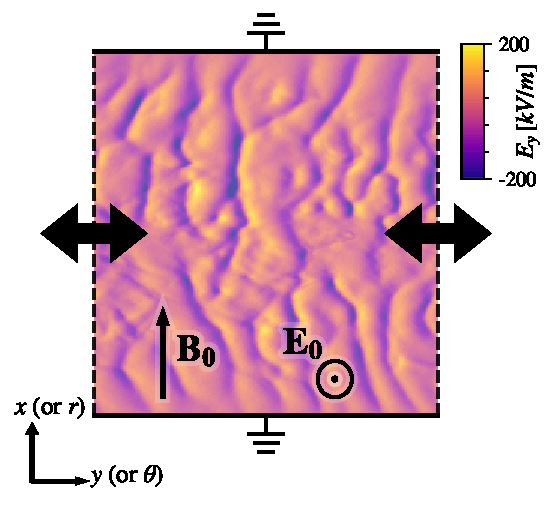
\includegraphics[width=\defaultwidth]{2D_schema.pdf}
  \caption{Schematic representation of the radial-azimuthal simulation domain. Overlaid is the computed azimuthal electric field given as an example. The radial dimensions lengths 2\,cm, and the azimuthal length is 1\,cm.
  The magnetic field is $B_0=0.02\,\tesla$, the axial electric field is $E_0=\sn{2}{4}\,\volt\per\meter$, and the walls are grounded. More parameters are given in \cref{parameters}.}
  \label{fig-2dschemat}
\end{figure}

\subsection{Particle balance}
As the axial position simulated is the exit plane, the ionization is too low to balance the particle losses to the wall.
Instead, the ionization takes place upstream, and the particles are convected downstream.
In these conditions, two models can be used concerning the particle losses at the walls\string:
\begin{itemize}
  \item having a simulation that dies off, as done in \citet{janhunen2018},
  \item forcing an arbitrary ionization to occur in order to compensate the radial losses \citep{dominguez-vazquez2018}.
\end{itemize}
The second option is slightly less realistic, but allows to obtain a steady-state and is supposed not to affect the simulation significantly.
Hence, we use this model to achieve a constant mean plasma density during the simulation.
The forced ionization rate is computed in order to compensate the losses of the ions at each time step.
The spacial ionization  profile is uniform.


\subsection{Axial convection}

Due to the imposed axial electric field, ions and electrons gain energy.
In the \ac{HET}, the axial convection of the particles balances the energy gain.
However, in a purely \ac{2D} simulations, the convection is missing, resulting in an ever-rising particle energy.
This prevents the possibility to reach a steady-state regime, as observed in \citet{heron2013,janhunen2018}.

We implemented a model of convection initially proposed for a \ac{1D} simulation by \citet{lafleur2016a}, and adapted in \ac{2D} by \citet{croes2017a}.
The model uses a finite axial length $L_z$.
When a particle reaches the boundary $z=0$ or $z=L_z$, it is removed from the simulation.
In order to conserve the particle (and charge) balance, a particle is created at $z=0$ for the ions (that are accelerated toward $z>0$) or at $z=L_z$ for the electrons.
It has been observed that using a radial position chosen uniformly at random for the newly injected particle would affect the sheath \citep{croes2017a}.
Hence, the radial position of the new particle is the same as the removed particle.

Concerning the azimuthal particle position, it is more difficult to choose between a random position or the same position as the removed particle.
In \citet{lafleur2016a,croes2017a}, a random azimuthal position was chosen.
However, as will be discussed in \cref{sec-reinjectionnoise}, this induces a numerical noise that can be harmful in some cases.

% !TEX root=/home/tavant/these/manuscript/src/manuscript.tex

\section{Dielectrics boundary condition}
  \label{sec-diel}

  \Cref{fig-2dschemat} shows the simulation of the radial-azimuthal domain with metallic grounded walls.
  \Cref{fig-2D} illustrates the configuration in the radial-azimuthal plane highlighting the more realistic radial boundary conditions.
  The plasma is bounded in the radial direction by dielectric layers isolating the magnetic circuit.
  The magnetic circuit can be considered electrically grounded.

  The particles are absorbed when touching the dielectric wall, and we suppose an infinite residence time.
  Hence, we obtain a surface charge $\sigma$ at a time $t$ with
  \begin{equation} \label{eq-sigmaintegrate}
    \sigma(t) = e \int_0^t (J_i - J_e) dt
  \end{equation}
  with $J_i$ and $J_e$ the ion and electron flux respectively and $e$ is the elementary charge and supposing that there is no surface charge at the interface at the beginning.

  \begin{figure}[hbt]
    \centering
    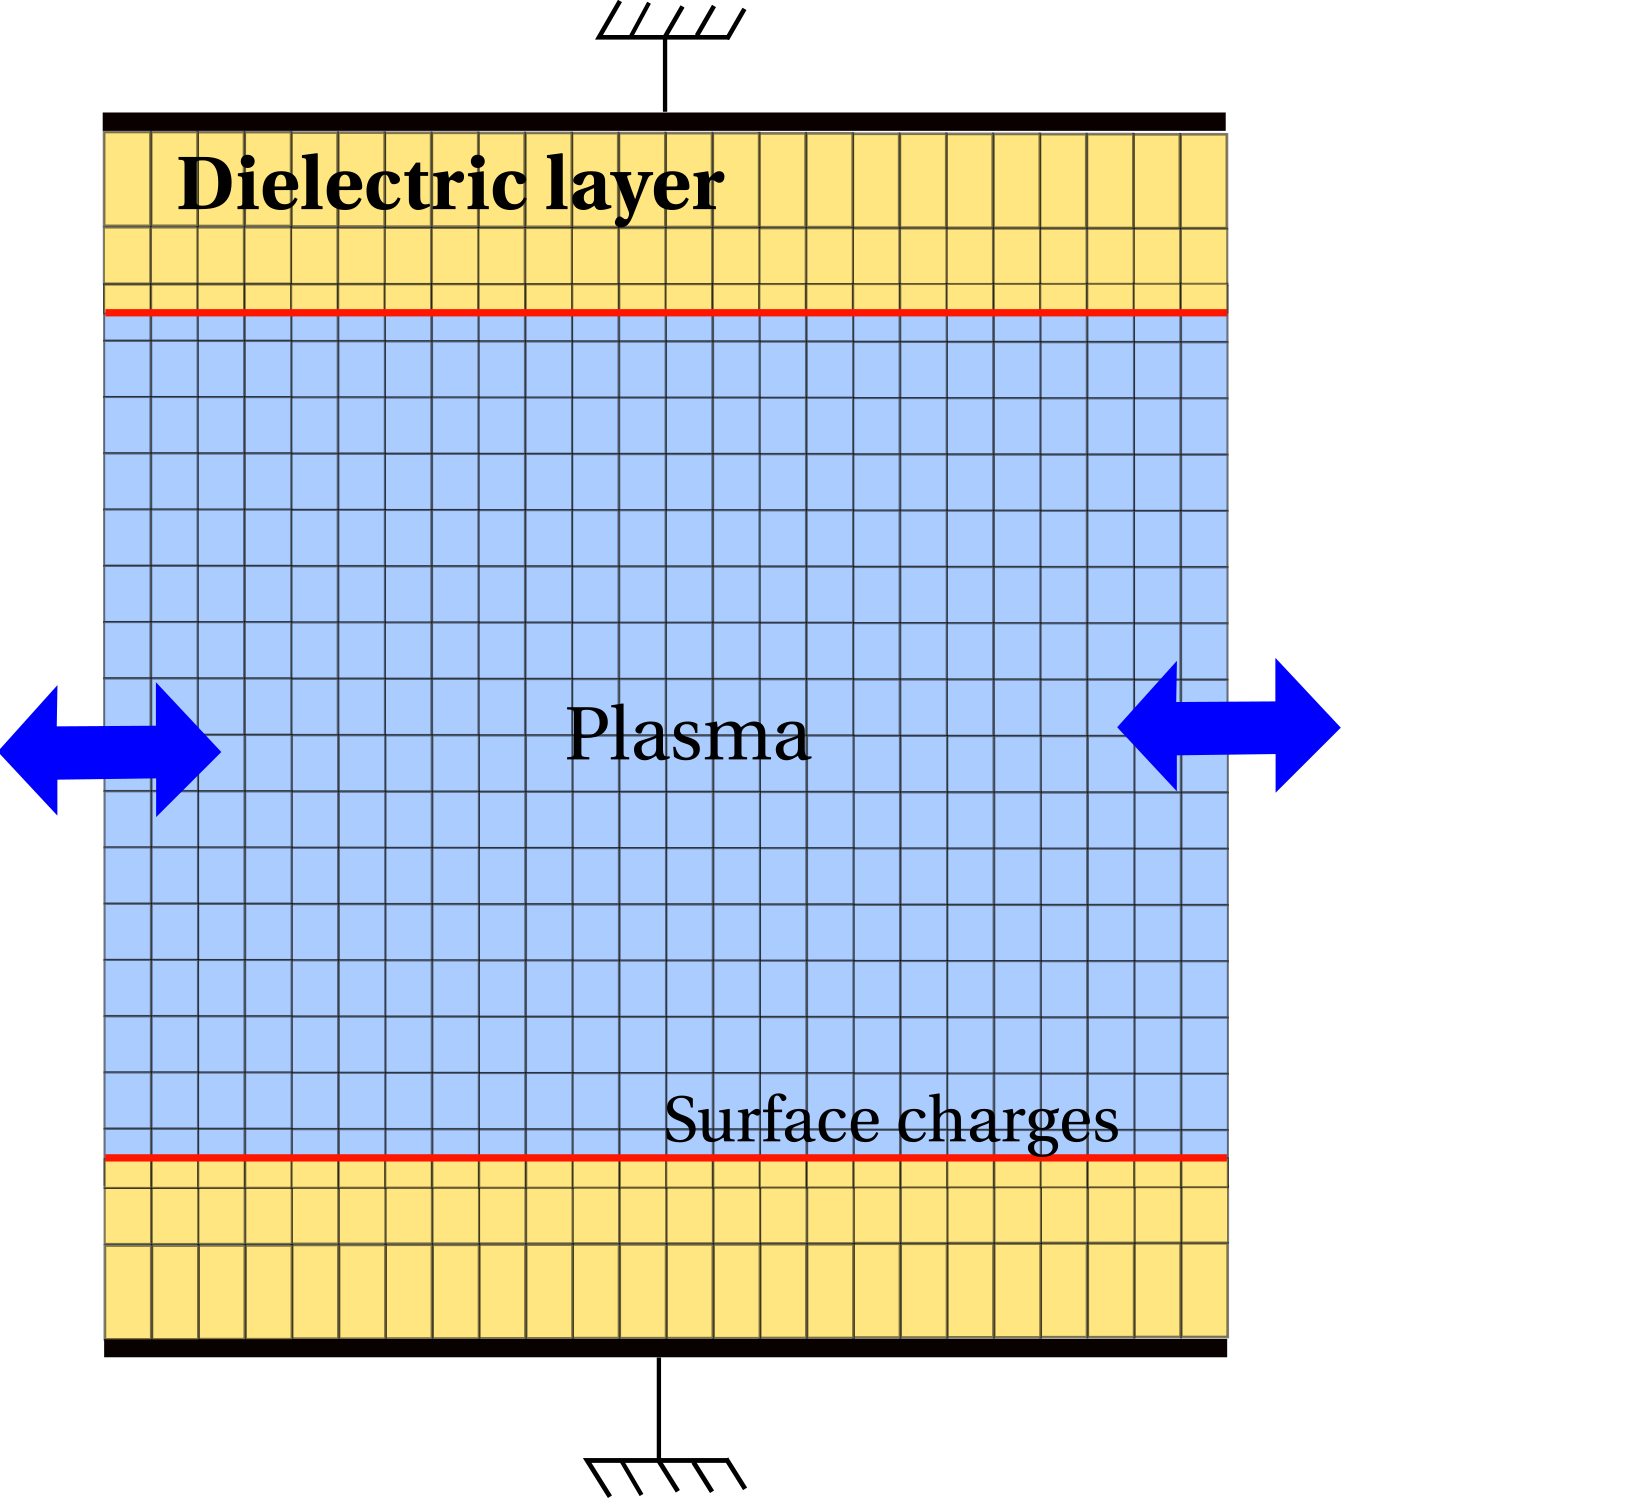
\includegraphics[width=\defaultwidth]{2D_diel_Rtheta}
    \caption{Schematic representation of the dielectric layers between the plasma in the \acs{2D} radial-azimuthal plane. Are present the dielectric in yellow, the plasma in blue, the surface charges in red, and the grounded magnetic circuit in black.}
    \label{fig-2D}
  \end{figure}


  A common approach is to assume that the electric field inside the dielectric is zero \citep{taccogna2019}. 
  Using Gauss theorem, we obtain a Neumann boundary condition at the plasma-wall interface for the potential
  \begin{equation} \label{eq-gauss}
    \norm{\partial_r \phi} = \frac{\norm{\sigma}}{\epsilon_0}
  \end{equation}
  with $\sigma$ the surface charge and $\epsilon_0$ the vacuum permittivity.
  However, the electric field in a dielectric material is not zero but depends on the global system.
  Hence, in order to model the dielectric wall of the \ac{HET} correctly, we choose to include the whole dielectric layers inside of the simulation domain.

  In this section, we derive the discretization of the Poisson equation with a non-uniform permittivity in the \ac{2D} radial azimuthal plane using the finite volume approach.


  \subsection{Non-uniform mesh}

    In the dielectric layers, there is no particle nor charge.
    Hence, the numerical constraints on the cell size are not applicable, and the cell size can be increased.
    In order to reduce the cell size difference between two neighboring cells, we use an exponential growth of the cell size in the radial direction.
    The cell size in the azimuthal direction $\dy$ is kept constant.
    The resulting non-uniform mesh can be seen in \cref{fig-2D}.


  \subsection{Poisson equation discretization}


  The dielectric permittivity is $\epsilon= \epsr \epsilon_0$ with $\epsr$ the relative permittivity of the dielectric.
  The Poisson equation with a not-constant permittivity is
  \begin{equation} \label{eq-poissondiel}
    \grad \cdot \epsilon \grad \phi = \rho
  \end{equation}
  with $\rho$ the charge density.
  We note $\vect{D}=\epsilon \vect{E} = \epsilon \grad \phi$ the electric flux.
  \Cref{fig-decompo1} shows the Cartesian decomposition of the \ac{2D} domain.
  The cell $(i,j)$ has four direct neighbors\string:
  \begin{itemize}
    \item the east $E$ in $(i+1,j)$
    \item the west $W$ in $(i-1, j)$
    \item the north $N$ in $(i, j+1)$
    \item the south $S$ in $(i, j-1)$
  \end{itemize}
  The cell dimensions are $\dx_{i,j}$ and $\dy_{i,j}$, and $\V=\dx_{i,j} \dy_{i,j}$ is the cell volume.
  As the mesh is Cartesian, we have for a given $j$ $\dx_{i,j} = cst$ for all $i$. Hence, we note $\dx_{i,j} = d_i$ and $\dy_{i,j} = d_j$

  The boundaries are noted $S^s_{i,j}$ with $s=E,W,N$ or $S$.
  We can see that $S^W_{i,j}=S^E_{i-1,j}$, and the same goes for the other borders.
  We note $\C = S^E_{i,j} \cup S^W_{i,j} \cup S^N_{i,j} \cup S^S_{i,j}$ the cell surface boundary.
  The center of the cell is located in $i,j$ and the borders are located in $i\pm 1/2$ in the East-West direction and $j\pm 1/2$ in the North-South direction.
  \begin{figure}[hbt]
    \centering
    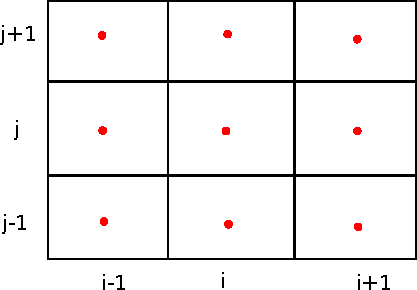
\includegraphics[width=\defaultwidth]{discrect1.pdf}
    \caption{Illustration of the Cartesian decomposition of the \acs{2D} domain}
    \label{fig-decompo1}
  \end{figure}


  \subsection{Poisson equation discretization}

    We start by positioning the plasma-dielectric interface on the surface between two cells.
    This means that the permittivity $\epsilon = \epsilon_0 \epsr$ is  constant over a cell.
    In order to discretize the Poisson equation, we integrate \cref{eq-poissondiel} over the cell volume

    \begin{equation}
    \int_{\V} - \grad \cdot (\epsilon \grad \phi) dv= \int_{\V} \rho dv.
    \end{equation}
    Using Gauss-Ostrogradsky theorem, we obtain
    \begin{equation}
    \oint_{\C} ( - \epsilon \grad \phi) \cdot \vect{n} dS = Q_{tot} =  \V \bar{\rho},
    \end{equation}
    with $\vect{n}$ the normal vector directed outward, $Q_{tot}$ is the total charge of the cell and $\bar{\rho}$ is the mean value of $\rho$ in the cell.
    We can decompose the integration over the cell boundary with the four surfaces $S^s_{i,j}$ as
    \begin{equation}
      \label{eq-poissonsum}
    \oint_{\C} (-\epsilon \grad \phi) \cdot \vect{n} dS = \sum_{k\in(E,W,N,S)} S^k_{i,j} \vect{D}^k_{i,j} \cdot \vect{n}
    \end{equation}
    with $\vect{D}^k_{i,j}$ the flux through the surface $k$ of the cell $(i,j)$.


    \paragraph*{Electric flux \\}
    Let us define the electric flux through the East border  $\vect{D}^E_{i,j}$.
    We suppose there is no surface charges on $S^E$.
    We can hence write the electric flux as
    \begin{align} \label{eq-flux1}
      \vect{D}^E_{i,j} \cdot \vect{n} &= \epsilon_{i,j} E_{x, i+1/2,j}^-\\
                                      &= - \epsilon_{i,j} \frac{\phi_{i+1/2,j} - \phi_{i,j}}{d_i/2},
    \end{align}
    with an off-center discretization of the electric field.
    Using the Gauss's law without charges
    \begin{equation} \label{eq-gausslaw}
      \epsilon_{i,j}E_{x, i+1/2,j}^- - \epsilon_{i+1,j}E_{x, i+1/2,j}^+ =0,
    \end{equation}
    we have
    \begin{equation}
      \epsilon_{i,j} \frac{\phi_{i+1/2,j} - \phi_{i,j}}{d_i/2} = \epsilon_{i+1,j} \frac{\phi_{i+1,j} - \phi_{i+1/2,j}}{d_{i+1}/2}.
    \end{equation}
    Hence
    \begin{equation} \label{eq-phidemi1}
      \phi_{i+1/2,j} = \frac{\epsilon_{i,j} d_{i+1} \phi_{i,j} + \epsilon_{i+1,j} d_{i} \phi_{i+1,j} }{\epsilon_{i,j} d_{i+1} + \epsilon_{i+1,j} d_{i} },
    \end{equation}
    which corresponds to the usual discretization \citep{croes2017} when $\epsilon$ and $d_i$ are both constant.
    Using \cref{eq-phidemi1} in \cref{eq-flux1} we obtain
    \begin{align}
      \label{eq-nosc}
    \vect{D}^E_{i,j} \cdot \vect{n} &=& 2\frac{\epsilon_{i,j}\epsilon_{i+1,j}}{\epsilon_{i,j}d_{i+1} + \epsilon_{i+1,j} d_i} (\phi_{i,j}-\phi_{i+1,j})
    &=& 2\epsilon_0 \frac{\epsr{i,j}\epsr{i+1,j}}{\epsr{i,j}d_{i+1} + \epsr{i+1,j} d_i} (\phi_{i,j}-\phi_{i+1,j})
    \end{align}

    We note $Q^E_{i,j} \equiv \frac{\epsilon_{i,j} \epsilon_{i+1,j}}{\epsilon_{i,j} d_{i+1} + \epsilon_{i+1,j} d_i}$.
    reproducing the same decomposition on the other borders, we obtain
    \begin{equation}
      \label{eq-descretPoisson1}
    S^E_{i,j} Q^E_{i,j} \phi_{i+1,j} + S^W_{i,j} Q^W_{i,j} \phi_{i-1,j} + S^N_{i,j} Q^N_{i,j} \phi_{i,j+1} + S^S_{i,j} Q^S_{i,j} \phi_{i,j-1} - Q^C_{i,j} \phi_{i,j} = - \V \bar{\rho_{i,j}}
    \end{equation}
    with
    \begin{center}
      $\begin{dcases}
     Q^E_{i,j} &= 2\frac{\epsilon_{i,j} \epsilon_{i+1,j}}{\epsilon_{i,j} d_{i+1} + \epsilon_{i+1,j} d_i} \\
     Q^W_{i,j} &= Q^E_{i-1,j} \\
     Q^N_{i,j} &= 2\frac{\epsilon_{i,j} \epsilon_{i,j+1}}{\epsilon_{i,j} d_{j+1} + \epsilon_{i,j+1} d_{j}}\\
     Q^S_{i,j} &= Q^N_{i-1,j} \\
     Q^C_{i,j} &= Q^E_{i,j}S^E_{i,j}+Q^W_{i,j}S^W_{i,j}+Q^N_{i,j}S^N_{i,j}+Q^S_{i,j}S^S_{i,j}
     \end{dcases}$
    \end{center}

    as well as $S^E_{i,j} = S^W_{i,j} =d_id_z, S^N_{i,j} = S^S_{i,j}= d_jd_z$ et $\V = d_jd_id_z$.
    We observe that the evolution of the relative permittivity and the cell size affects the coefficients to be used, but the system remains symmetric as we have $Q^S_{i,j} = Q^N_{i-1,j}$ and $ Q^W_{i,j} = Q^E_{i-1,j}$.
    
    A symmetric system is a linear system of equation $A \cdot X = B$  which matrix $A$ is equal to its transpose\string: $A = A^T$.
    It allows reducing by a factor of two the memory needed to store the matrix.
    It also allows to use algorithms exploiting this aspect.
    For instance, the eigenvalues are real-valued, and the matrix factorization only need to store one factor using Cholesky decomposition, which gives $A = L L^T$ with $L$ a lower-triangular matrix. 

    \subsection{Including surfaces charges}
    Let's now considerer the presence of surface charges on the surface $S^E_{i,j}$.
    Gauss's law now reads
    \begin{equation} \label{eq-gausslawsc}
      -\epsilon_{i,j}E_{x, i+1/2,j}^- + \epsilon_{i+1,j}E_{x, i+1/2,j}^+ =\sigma^E,
    \end{equation}
    with $\sigma^E$ the surface charge on the surface.
    The surface charge is not taken into account when computing the total charge in a cell.
    Using the same discretization as before, we obtain
    \begin{equation}
    \epsilon_{i,j} \frac{\phi_{i+1/2,j} - \phi_{i,j}}{d_i/2} - \epsilon_{i+1,j} \frac{\phi_{i+1,j} - \phi_{i+1/2,j}}{d_{i+1}/2} = \sigma^E
    \end{equation}
    so that
    \begin{equation}
      \label{eq-phidemi}
    \phi_{i+1/2,j} = \frac{\epsilon_{i,j} d_{i+1} \phi_{i,j} + \epsilon_{i+1,j} d_{i} \phi_{i+1,j} }{\epsilon_{i,j} d_{i+1} + \epsilon_{i+1,j} d_{i} } + \frac{1}{2}\sigma^E \frac{d_i d_{i+1}}{\epsilon_{i,j} d_{i+1} + \epsilon_{i+1,j} d_{i}}
    \end{equation}
    hence
    \begin{align*}
    \vect{D}^E_{i,j} \cdot \vect{n} &= 2\frac{\epsilon_{i,j}\epsilon_{i+1,j}}{\epsilon_{i,j}d_{i+1} + \epsilon_{i+1,j} d_i} (\phi_{i,j}-\phi_{i+1,j}) - \sigma^E \frac{\epsilon_{i,j}d_{i+1}}{\epsilon_{i,j}d_{i+1}+\epsilon_{i+1,j}d_{i}}
    \end{align*}
    We obtain the same relation that \cref{eq-nosc} updated by $- \sigma^E \frac{\epsilon_{i,j}d_{i+1}}{\epsilon_{i,j}d_{i+1}+\epsilon_{i+1,j}d_{i}}$

    Hence, we finally obtain
    \begin{equation}
    S^E_{i,j} Q^E_{i,j} \phi_{i+1,j} + S^W_{i,j} Q^W_{i,j} \phi_{i-1,j} + S^N_{i,j} Q^N_{i,j} \phi_{i,j+1} + S^S_{i,j} Q^S_{i,j} \phi_{i,j-1} - Q^C_{i,j} \phi_{i,j} = - \V \bar{\rho_{i,j}} + Q^W_{\sigma} \sigma^W
    \end{equation}
    with $Q^W_{\sigma} =  S^W_{i,j} \frac{\epsilon_{i,j}d_{i-1}}{\epsilon_{i,j}d_{i-1}+\epsilon_{i-1,j}d_{i}}$.



  \subsection{Verification of the Poisson solver} \label{subsec-poisson_validation}
    We verify the discretization by modeling a \ac{1D} capacitor.
    The length of system is $L=1\,\meter$.
    The relative permittivity of the dielectric inside the capacitor (from $x=0.475$ to $0.525\,\meter$) is set to $\epsr = 8$, and a surface charge of  $\sigma = 8$~nC.cm$^{-2}$ is imposed on one side, and $-8$~nC.cm$^{-2}$ on the other side.
    The expected electric field in the capacitor using the infinite plane approximation is $E = \sigma/(\epsilon_0\epsr) = 1.15$~kV.mm$^{-1}$.

    \Cref{fig-surface} shows the electric field computed using the obtained decomposition
    We see that we obtain the expected jump for the electric field due to the surface charge ($\Delta E = 1.15$~kV/m).
    The difference with the theoretical value is due to the Dirichlet conditions $\phi=0$ used in $x=0$ and $x=1\,\meter$.
    

    \begin{figure}[hbt]
      \centering
      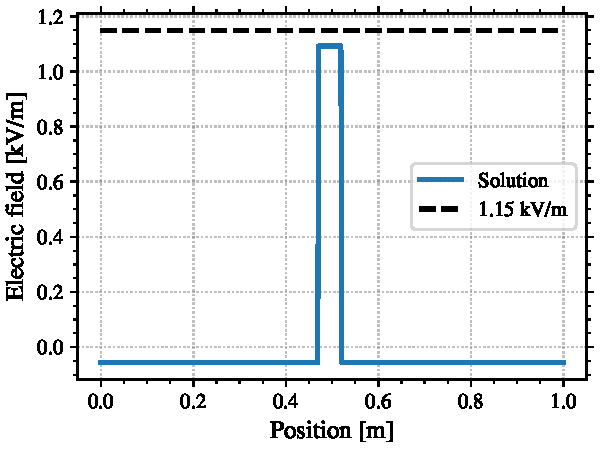
\includegraphics[width=\defaultwidth]{validation_dielectric_field.pdf}
      \caption{Electric field of the capacitor configuration calculated by the Poisson solver in order to validate the discretization and the solver developed. }
      \label{fig-surface}
    \end{figure}



  \subsection{Interface at the cell center}
    In the previous section, we supposed that the plasma-dielectric dielectric boundary was at the interface between the cells.
    However, this means that the electric field close to the interface is unknown, as it is defined at the cell center.
    Moreover, the Dirichlet condition for the potential is better defined at the cell center, and for the sake of simplicity, changing the boundary conditions should not change the particle domain.
    Hence, we chose to position the plasma-wall interface at the center of the cell as shown in \cref{fig-2D,fig-decompo2}.
    This means that the permittivity is not constant over a cell.

    Because the wall boundaries are only in the radial direction, we consider only an interface in the North-South direction.
    \Cref{fig-decompo2} shows the domain decomposition.
    The decomposition is the same as previously, except for the permittivity that can have two different values\string: one in the North half-plane ${\epsr}_{, i,j}^n$ and another in the South half plane ${\epsr}_{, i,j}^s$.

    \begin{figure}[hbt]
      \centering
      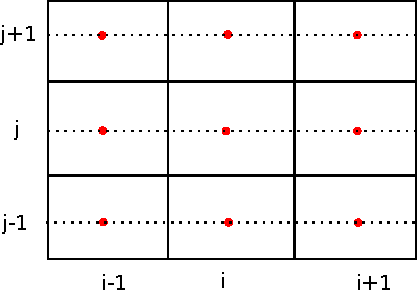
\includegraphics[width=\defaultwidth]{discrect2.pdf}
      \caption{Cartesian decomposition of the \acs{2D} domain. The dash lines represent discontinuities in the permittivity value.}
      \label{fig-decompo2}
    \end{figure}

    The discretization of the Poisson \cref{eq-poissonsum} follows the same path as previously, except that the electric flux in not constant anymore so that \cref{eq-poissonsum} becomes
    \begin{equation}
    \oint_{\C} (-\epsilon \grad \phi) \cdot \vect{n} dS = \sum_{k\in(E,W,N,S)} S^k_{i,j} <\vect{D}^k_{i,j} \cdot \vect{n}>.
    \end{equation}

    We can define
    \begin{align}
    <\vect{D}^E_{i,j} \cdot \vect{n} >&= \frac{1}{2} \epsilon_{i,j}^N E_{x, i+1/2,j}^- + \frac{1}{2} \epsilon_{i,j}^S E_{x, i+1/2,j}^-\\
     &= \frac{-1}{2} (\epsilon_{i,j}^N + \epsilon_{i,j}^S) \frac{\phi_{i+1/2,j} - \phi_{i,j}}{d_i/2}
     \label{eq-flux}
    \end{align}
    so that in the East-West direction, the flux behaves as if the cell permittivity is the mean of the North and South half-plane  $\epsilon_{i,j} = \frac{1}{2} (\epsilon_{i,j}^N + \epsilon_{i,j}^S)$.
    Hence, the rest of the computation is similar.
    For the boundary North and South, the permittivity is constant, hence there is no modification.
    Consequently, we obtain the discretization
    \begin{equation}
    S^E_{i,j} Q^E_{i,j} \phi_{i+1,j} + S^W_{i,j} Q^W_{i,j} \phi_{i-1,j} + S^N_{i,j} Q^N_{i,j} \phi_{i,j+1} + S^S_{i,j} Q^S_{i,j} \phi_{i,j-1} - Q^C_{i,j} \phi_{i,j} = - \V \bar{\rho_{i,j}}
    \label{eq-descretPoissoncentred}
    \end{equation}
    with
    \begin{center}
     $\begin{dcases}
     Q^E_{i,j} &= 2\frac{\epsilon_{i,j} \epsilon_{i+1,j}}{\epsilon_{i,j} d_{i+1} + \epsilon_{i+1,j} d_i} \\
     Q^W_{i,j} &= Q^E_{i-1,j} \\
     Q^N_{i,j} &= 2\frac{\epsilon_{i,j}^N \epsilon_{i,j+1}^S}{\epsilon_{i,j}^N d_{j+1} + \epsilon_{i,j+1}^S d_{j}}\\
     Q^S_{i,j} &= 2\frac{\epsilon_{i,j}^S \epsilon_{i,j-1}^N}{\epsilon_{i,j}^S d_{j+1} + \epsilon_{i,j-1}^N d_{j}} \\
     Q^C_{i,j} &= Q^E_{i,j}S^E_{i,j}+Q^W_{i,j}S^W_{i,j}+Q^N_{i,j}S^N_{i,j}+Q^S_{i,j}S^S_{i,j}
     \end{dcases}$
    \end{center}

    As well as $S^E_{i,j} = S^W_{i,j} =d_id_z, S^N_{i,j} = S^S_{i,j}= d_jd_z$ et $\V = d_jd_id_z$.
    Here, the system is no more symmetric.
    However, we can suppose that the only permittivity jump happens at the cell center, so that  $\epsilon_{i,j}^S = \epsilon_{i,j-1}^N$.
    Hence, $Q^N_{i,j} = 2\frac{\epsilon_{i,j}^N}{ d_{j+1} + d_{j}}$ and the system is symmetric.

  \subsection{Surface charges for centred interface}
    in the case of centred plasma-wall interface, we have surfaces charges at the center of the cell.
    Hence
    \begin{equation}
    \int_{\Omega_{i,j}} \rho dv = \Omega_{i,j}\bar{\rho} + S_{i,j}^N \sigma_{i,j}.
    \end{equation}
    The surface charges behave like volume charges.
    Hence, we obtain
    \begin{equation}
    S^E_{i,j} Q^E_{i,j} \phi_{i+1,j} + S^W_{i,j} Q^W_{i,j} \phi_{i-1,j} + S^N_{i,j} Q^N_{i,j} \phi_{i,j+1} + S^S_{i,j} Q^S_{i,j} \phi_{i,j-1} - Q^C_{i,j} \phi_{i,j} = - \V \bar{\rho_{i,j}} - S^N_{i,j} \sigma_{i,j}
    \end{equation}

    The discretization obtained for the plasma-wall interface cell-centred is very similar to the one obtained for the interface at the cell interface.
    However, it conserves the particle domain when the dielectric layer is not modeled, and that Dirichlet conditions are applied, and the electric field at the plasma-wall interface is better defined.
    Hence, the cell-centred interface will be used.

    \vspace{1em}
    This decomposition has been validate with the same test than presented in \cref{subsec-poisson_validation}.
    We observed no difference between the two decompositions in term of precision.
    
    
  \subsection{Electric field computation}
  
    The resolution of the Poisson equation returns the value of the plasma potential $\phi$ at the cell centers.
    The electric field is computed by taking the first derivative of the potential at the cell interface, as in \cref{eq-flux1},
    \begin{equation} \label{eq-E_ihalf}
      E_{x, i+1/2,j}^- = - \epsilon_{i,j} \frac{\phi_{i+1/2,j} - \phi_{i,j}}{d_i/2},
    \end{equation}
    with $\phi_{i+1/2,j}$ defined with \cref{eq-phidemi1}.
    However, in order to have consistent data, the electric field is also computed at the cell center by interpolation
    \begin{equation} \label{eq-E_mean}
      E_{x, i, j} = \frac{1}{2} \lp E_{x, i-1/2,j} + E_{x, i+1/2,j} \rp =  - \epsilon_{i,j} \frac{\phi_{i+1/2,j} - \phi_{i-i/2,j}}{d_i}.
    \end{equation}
    
    In the cells along to the plasma-wall interface, the effect of the surface charge must be taken into account, is previously described.
    
    \improvement{Can be more explicit here. Add exact expression of $E$ with $\phi_{i,j}$ and the effect of the surface charge.}
  
  
  
% !TEX root=/home/tavant/these/manuscript/src/manuscript.tex

\section{Axial Convection model}
  \label{sec-reinjectionnoise}

  As introduced in the previous section, the \ac{2D} radial-azimuthal simulation does not model a priori the axial convection of the particles.

  \subsection{Lafleur's model of convection}

    \citet{lafleur2016a} proposed a way to model the axial convection of the particles in a \ac{1D} purely azimuthal simulation.
    \Cref{fig-Fake_1d_1} shows a schematic illustration of the model.
    The principle is as follow
    \begin{itemize}
      \item We set a finite axial length, noted $L_z$ on \cref{fig-Fake_1d_1}.
      \item We follow the positions of the particle in the axial direction $z$
      \item When a particle crosses the boundary, it is removed.
      \item A new particle is created
      \begin{itemize}
        \item at $z=0$ for the ions
        \item  at $z=L_z$ for the electrons
      \end{itemize}
    \end{itemize}

    We create a new particle in order to conserve the charge in the simulation.
    The new particle has a velocity following a Maxwellian flux distribution function of a given temperature.
    The azimuthal position of the particle is chosen uniformly at random.

    \improvement{Add definition of the Maxellian and maxellian flux VDF ?}

    \begin{figure}[hbtp]
      \centering
      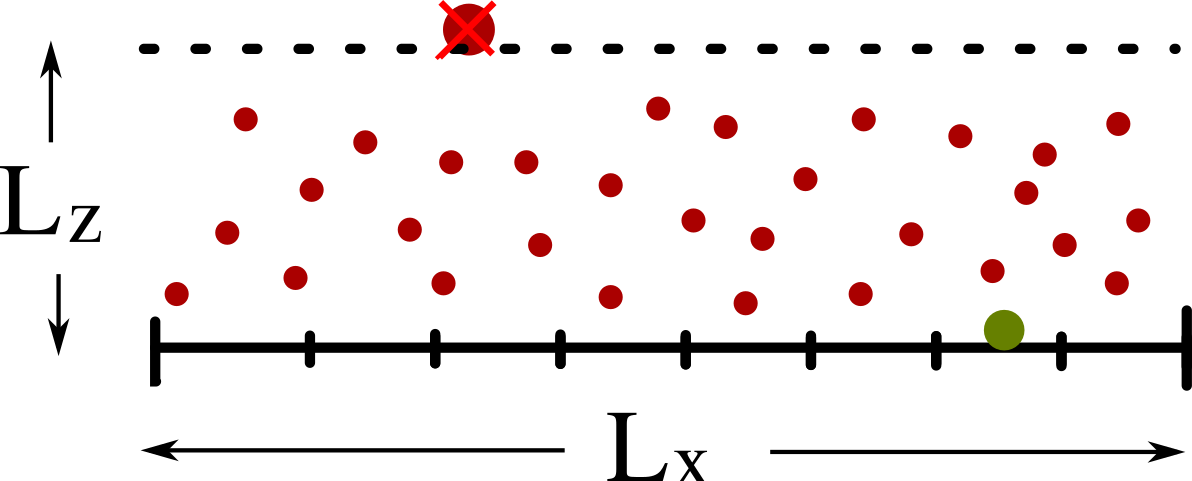
\includegraphics[width=\defaultwidth]{Fake_1d_2}
      \caption{Schematic representation of Lafleur's convection model \citep{lafleur2016a}. The red particle is removed of the simulation, and the green particle is created. In this illustration, the particle is an ion, and the reinjection is at $z=0$. }
      \label{fig-Fake_1d_1}
    \end{figure}

    Lafleur's model of convection has been adopted in \ac{2D} by \citet{croes2017a}.
    The principle is exactly similar.
    The particles are followed in the 3 directions, and a finite length is used to close to axial direction.
    It is important to note that even is the particle are followed in the 3 directions, the meshed domain is only \ac{2D}.
    The simulation is not \ac{3D}-\ac{3V}, but only \ac{2D}-\ac{3V}.

    In \citet{croes2017a}, the authors have observed that if the newly created particle has a radial position chosen uniformly at random, it would affect the sheath.
    Hence, they decided to use the same radial position that the removed particle.
    \Cref{fig-Fake_2d} presents a schematic representation of the convection model in \ac{2D}.

    \begin{figure}[hbtp]
      \centering
      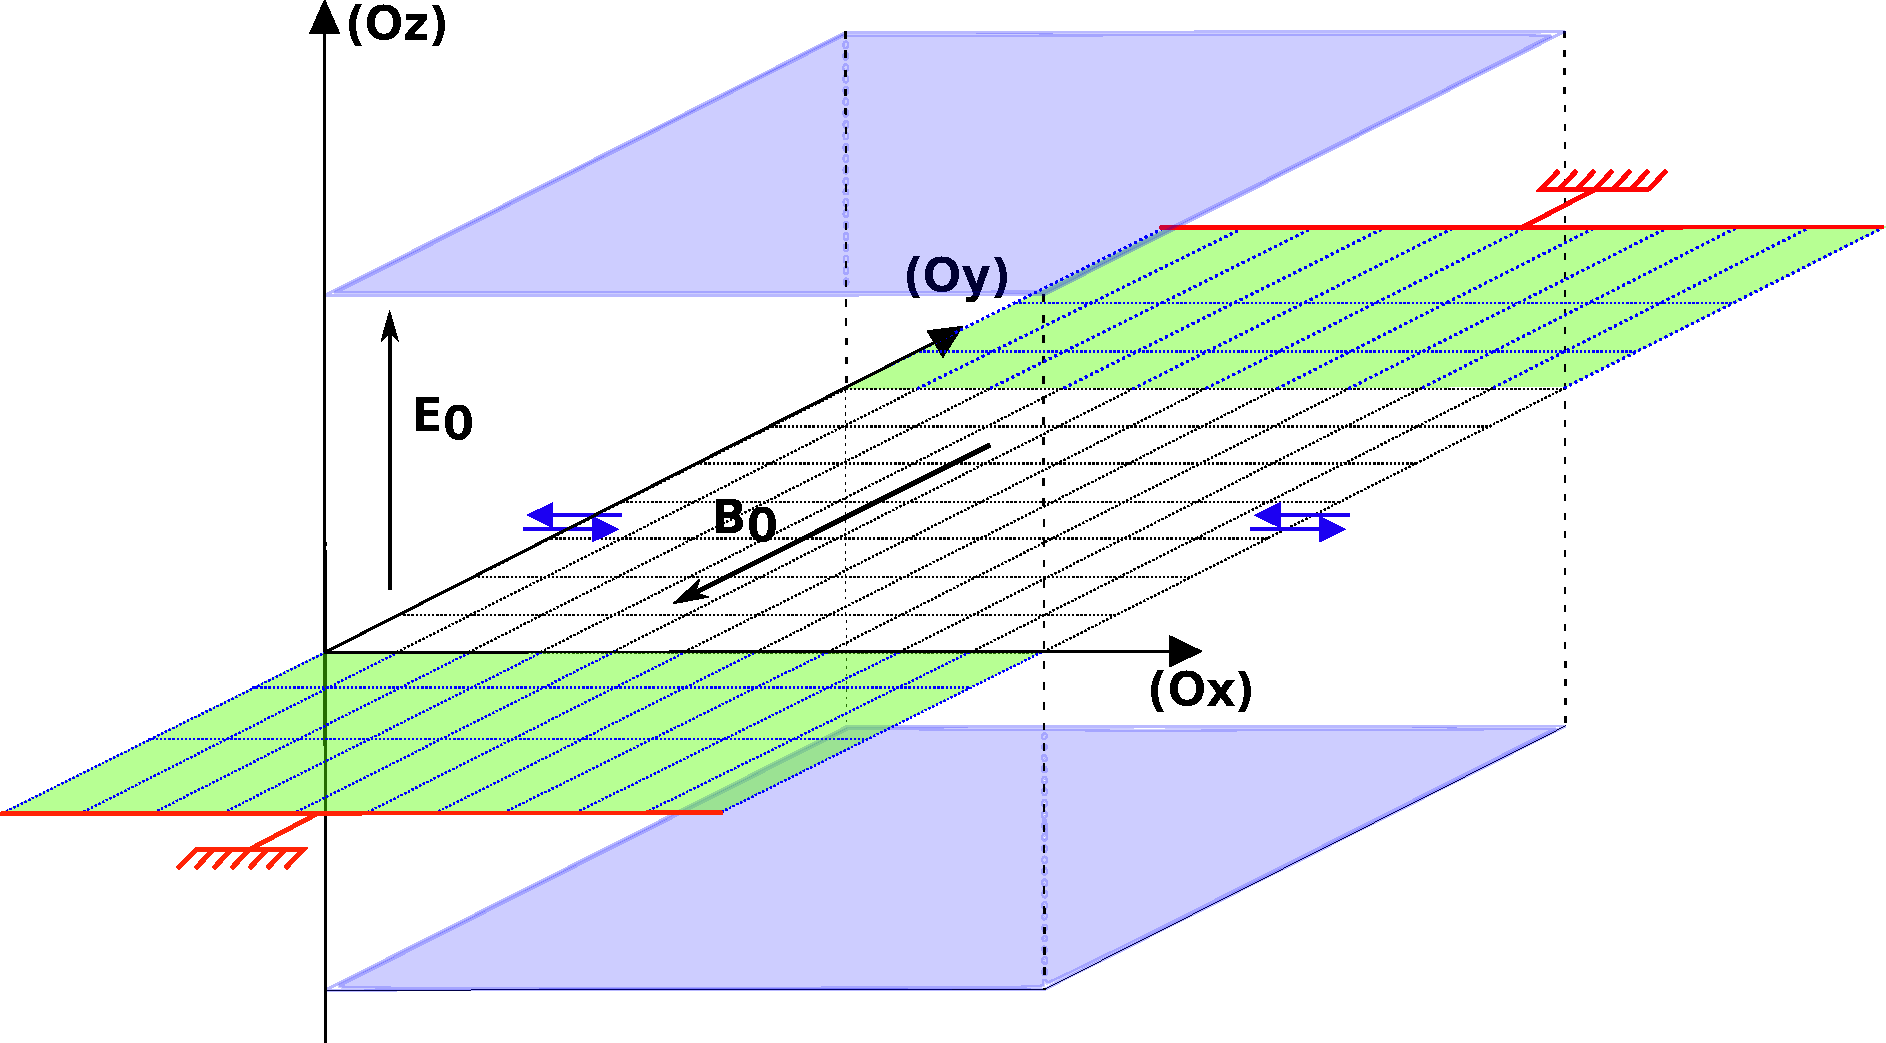
\includegraphics[width=\defaultwidth]{2_5D_dielectric_PPS_small}
      \caption{Schematic representation of the Lafleur's convection model adapted in \ac{2D}. The new particle radial position corresponds to the removed particle, but its azimuthal position is chosen uniformly at random. }
      \label{fig-Fake_2d}
    \end{figure}

    \Cref{fig-energy_convection} shows the evolution as a function of time of the electron mean energy in the simulation in a typical \ac{2D} radial-azimuthal simulation, addapted from \citet{croes2017}.
    We can see that without the convection, the mean energy quickly rises to unphysical values.
    When the convection is modeled, using an axial of $L_z=1$ cm, the energy reaches a steady state.
    \nomenclature[Q]{\ensuremath{ L_z}}{ Axial length}
    \begin{figure}[hbtp]
      \centering
      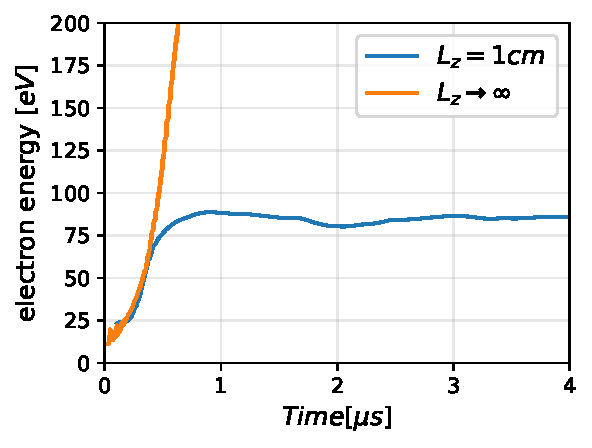
\includegraphics[width=\defaultwidth]{energy}
      \caption{Time evolution of the electron mean energy when the convection is not modeled ($L_z \rightarrow \infty$) and with Lafleur's convection model used, $L_z = 1$ cm. Adapted from \citet{croes2017}.}
      \label{fig-energy_convection}
    \end{figure}



  \subsection{Numerical artefacts}
    \citet{lafleur2016a} studied the impact of the convection model on the simulation results.
    The authors observed in particular that changing the azimuthal length of the simulation domain could affect the simulation results.

    \Cref{fig-convection_numerical} shows the time evolution of the azimuthal electric field $E_{\theta}$ from the \ac{1D} simulation \citep{lafleur2016a}.
    \nomenclature[Q]{\ensuremath{ E_{\theta}}}{ Azimuthal electric field}

    On the first row (\cref{fig-convection_numerical}.{\bf a} and {\bf b}), the length of the periodic azimuthal direction is $L_{\theta}=0.5$~cm.
    \cref{fig-convection_numerical}.{\bf a} corresponds to the case without axial convection.
    We clearly see that the \ac{ECDI} rises and does not saturate.
    The wavelength is short, of the order of $\lambda = 1.5$~mm.
    \nomenclature[Q]{\ensuremath{ \lambda}}{ Wave length}
    \cref{fig-convection_numerical}.{\bf b} corresponds to the same case as \cref{fig-convection_numerical}.{\bf a} but this time with the axial convection modeled.
    We observe this time a saturation of the oscillation's amplitude, and the wavelength is close to $\lambda \simeq 1.5$~mm.

    On the second row (\cref{fig-convection_numerical}.{\bf c} and {\bf d}), the length of the periodic azimuthal direction is $L_{\theta}=1$~cm.
    \cref{fig-convection_numerical}.{\bf c} corresponds to the case without axial convection, and \cref{fig-convection_numerical}.{\bf b} corresponds to the same case but with the axial convection modeled.
    In \cref{fig-convection_numerical}.{\bf c}, we can see that increasing the azimuthal length did not affect the \ac{ECDI}, as expected.
    However, in  \cref{fig-convection_numerical}.{\bf d}, the instability is clearly affected.
    A single oscillation is observed, corresponding to $\lambda=10$~mm, which seems almost certainly unphysical.

    \begin{figure}[hbtp]
      \centering

      \begin{tabular}{cc}
        \subfigure{Lafleur_NoLz_1}{a}{20, 20}
            &
        \subfigure{Lafleur_Lz_1}{b}{20, 20} \\

        \subfigure{Lafleur_NoLz_2}{c}{20, 20} &
        \subfigure{Lafleur_Lz_2}{d}{20, 20} \\
      \end{tabular}
      \caption{Effects of Lafleur's convection model for two different azimuthal length on the azimuthal electric field. ({\bf a}) No convection, $L_x=0.5$~cm,  ({\bf b}) convection modeled, $L_x=0.5$~cm,  ({\bf c}) No convection, $L_x=1$~cm,  ({\bf d}) convection modeled, $L_x=1$~cm. The colour of each plots is normalized to the maximum amplitude. Adapted from \citep{lafleur2016a}. \inlinenote{Get $\theta$ back to $y$ instead of $x$}}
      \label{fig-convection_numerical}
    \end{figure}

    \FloatBarrier
    \citet{croes2017} observed similar behaviour with the bidimensional  simulation.
    The author investigated the values of the azimuthal length which presented physical and unphysical results
    for different values of the axial length.
    \Cref{fig-couplesCroes} shows the results obtained (adapted from \citep{croes2017}).
    We can see that for a given value of the axial length, the azimuthal must be less that a certain value to present physical results.
    However, the value of this upper limit depends of the axial length, such that the if the axial length decreases, the upper limit of the azimuthal length decreases as well.

    \begin{figure}[hbtp]
      \centering
      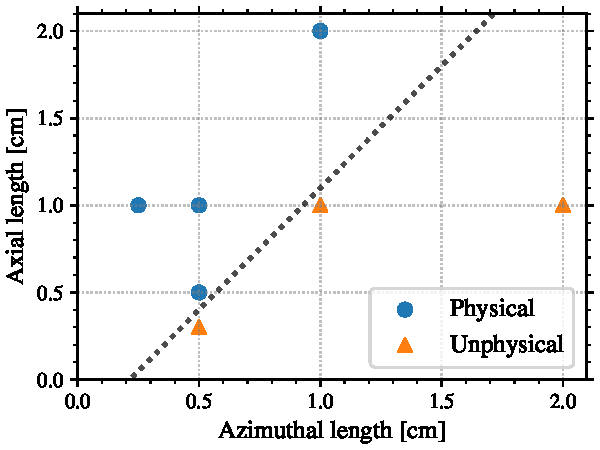
\includegraphics[width=\defaultwidth]{2D_couples}
      \caption{Values of the azimuthal length and the axial length for which the simulation result is physical (similar to \cref{fig-convection_numerical}.{\bf b}) or unphysical  (similar to \cref{fig-convection_numerical}.{\bf d}) \inlinenote{Make this image smaller (smaller font, etc.), correct azimuthal}}
      \label{fig-couplesCroes}
    \end{figure}

    In the next section, we develop a theory that could explain the observation, and a new convection model for the simulation is proposed.

  \subsection{Numerical noise of Lafleur's convection model}

    Let us consider Lafleur's convection model in \ac{1D} on the charge density.
    When computing the charge density on the mesh vertices, the axial position is not taken into account.
    Consequently, the convection process illustrated on \cref{fig-Fake_1d_1} is similar to moving a particle arbitrarily (read randomly).
    Seen by the charge density, this is similar to a Poisson noise, also named shot noise, on the charge density.\footnote{Actually, this noise is the combination of a Poisson noise with a uniform noise, happening twice for every particles convection, once with a positive charge and once with a negative charge.}

    After a certain number of particles removed and created, the Poisson noise is similar to a Gaussian noise, also named thermal noise, following a normal distribution $\N$ . 
    \nomenclature[Q]{\ensuremath{ \N }}{ Normal distribution.}
    Hence, the charge density becomes \footnote{One can note that the mean of the noise is strictly zero (with probability 1), as the charge density is conserved.}
    \begin{equation} \label{eq-rhonoise}
      \rho = \rho_0 + \N(0, \stdconv),
    \end{equation}
    with $\rho$ the charge density, $\rho_0$ the charge density without the convection process, and $\stdconv$ the standard deviation of the distribution of the noise associated with the convection model.
    \nomenclature[Q]{\ensuremath{ \rho}}{ Charge density}
    \nomenclature[Q]{\ensuremath{ \stdconv}}{ tandard deviation of the distribution of the noise associated with the convection model}
    Surprisingly, the noise due to the convection model is similar to the numerical noise induced by the decomposition of the plasma into particles $\N(0, \sigma_{\rm stat})$.
    However, the amplitude of this statistical noise decreases with the number of particles per cell used
    \begin{equation*} \label{eq-statistical}
     \sigma_{\rm stat} \propto \frac{1}{\sqrt{N_{pc}}}.
    \end{equation*}

    On the other hand, the amplitude of the noise induced by the convection model depends on the plasma density $n$, the axis velocity of the particles $v_z$ and the axial length $L_z$
    \begin{equation} \label{eq-convstd}
     \stdconv \propto \frac{n}{L_z} v_z.
    \end{equation}

    We can see on \cref{eq-convstd} that the amplitude of the convection induced noise on the charge density is proportional to the inverse of the axial length $L_z$.
    This could explain the observation of \cref{fig-couplesCroes} when using a smaller $L_z$.
    However, it does not explain the effects of the azimuthal length observed in \cref{fig-couplesCroes,fig-convection_numerical}.

  \subsection{Effect of the noise on the electric field}
    \label{sec-mathnoise}
    In order to explain the impact of the azimuthal length on the instability, we can study the azimuthal electric field $\aziE$ resulting of the charge density $\rho$.
    As the Pouisson equation is linear, we have
    \begin{align}
      \aziE(\theta) &= C + \frac{1}{\epsilon_0} \int_0^{\theta} \rho(s) ds\\
                    &= C + \frac{1}{\epsilon_0} \int_0^{\theta} (\rho_0(s) + \N(0, \stdconv) ) ds \\ 
                    &= C + \aziE_{, 0} + \aziE_{, 1}
    \end{align}
    with $C$ a constant that ensure that the periodical \ac{BC} are respected.
    The part of the electric field $\aziE_{, 0}$ corresponds to the unperturbed charge density $\rho_0$ and $\aziE_{, 1}$  corresponds to the noisy charge density $\N(0, \sigma_{\rm stat})$.
    Hence, let us focus now on $\aziE_{, 1}$.
    We can study $\aziE_{, 1}$ using two equivalent means\string: the \ac{FT} and the Brownian bridge.
    
    \paragraph{Fourier Transform \\}
      Applying the \ac{FT} on the equation
      \begin{equation} \label{eq-aziE1}
        \aziE_{, 1} = \frac{1}{\epsilon_0} \int_0^{\theta}  \N(0, \stdconv) ds
      \end{equation}
      gives    
      \begin{align}
        \FFT \lp \aziE_{, 1} \rp (k) &= \frac{1}{\epsilon_0} \FFT \lp \int_0^{\theta}  \N(0, \stdconv) ds \rp \\
                                     &= \frac{1}{\epsilon_0} \frac{ \N(\mu_{\rm FT}, \sigma_{\rm FT})}{k} \label{eq-fft}
      \end{align}
      
      \Cref{eq-fft} shows that $\aziE_{, 1}$ is also follows a Gaussian distribution, but with a non-zero mean value.
      It is also inversely proportional to the wave number $k$.
      Hence, when we increase the azimuthal length, which means that small wave number can exit in the simulation domain, the amplitude of $\aziE_{, 1}$ increases as well.
      
    \paragraph{Brownian Bridge\\}
      \Cref{eq-aziE1}, combined with the \ac{BC}, is the definition of the a Browning bridge.
      
      A Brownian bridge is a particular Brownian motion that reaches at a given distance the same value that the initial value.
      Hence, we have \citep{ibe2013}
      \begin{align*}
        \mathbb{E}(\aziE_{, 1}) &= 0,  \\
        {\rm var}(\aziE_{, 1}) &= \stdconv^2 \frac{L_{\theta}}{4}
      \end{align*}
    
      Hence, the increase of the azimuthal length increases the amplitude of $\aziE_{, 1}$.
      
    
    We believe that when the amplitude of $\aziE_{, 1}$ is too large, it can trigger an unphysical oscillation.
    The next section uses this conclusion in order to adapt the convection model.
    
    \subsection{Noiseless convection model}
      \label{sec-noiselessresults}
      In previous section, we have shown that the convection model induces a noise in the charge density, that produces an azimuthal electric field which amplitudes depends on the azimuthal length.
      
      We propose here a modified version of Lafleur's convection model in order to remove the noise in the charge density
      The noiseless convection model follows the same algorithm that before, but the azimuthal position of the particle created is not chosen uniformly as random, but instead the new particle has the same position as the removed particle.
      \Cref{fig-fakez3} shows a schematic illustration of the noiseless convection algorithm applied on a particle.
      
      \begin{figure}[hbtp]
        \centering
        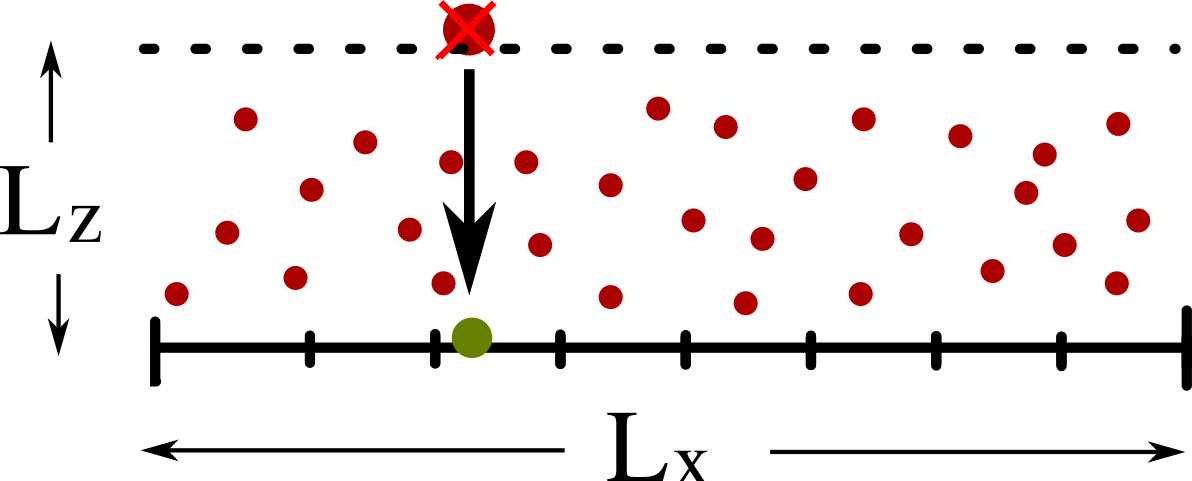
\includegraphics[width=\defaultwidth]{Fake_1d_3}
        \caption{Illustration of the noiseless convection model}
        \label{fig-fakez3}
      \end{figure}
      
      We have implemented this modified convection model in the \ac{2D} radial-azimuthal simulation.
      
      \Cref{fig-newconv_noconv} shows the time  evolution of the azimuthal electric field at the center of the radial dimension with and without the noiseless convection model.
      It presents the same conditions that in \cref{fig-convection_numerical}.{\bf a} and {\bf b}. 
      As previously, the convection stabilises the growth of the instability to a steady-state, but it does not affect the physics.
       
      
      \begin{figure}[hbtp]
        \centering
        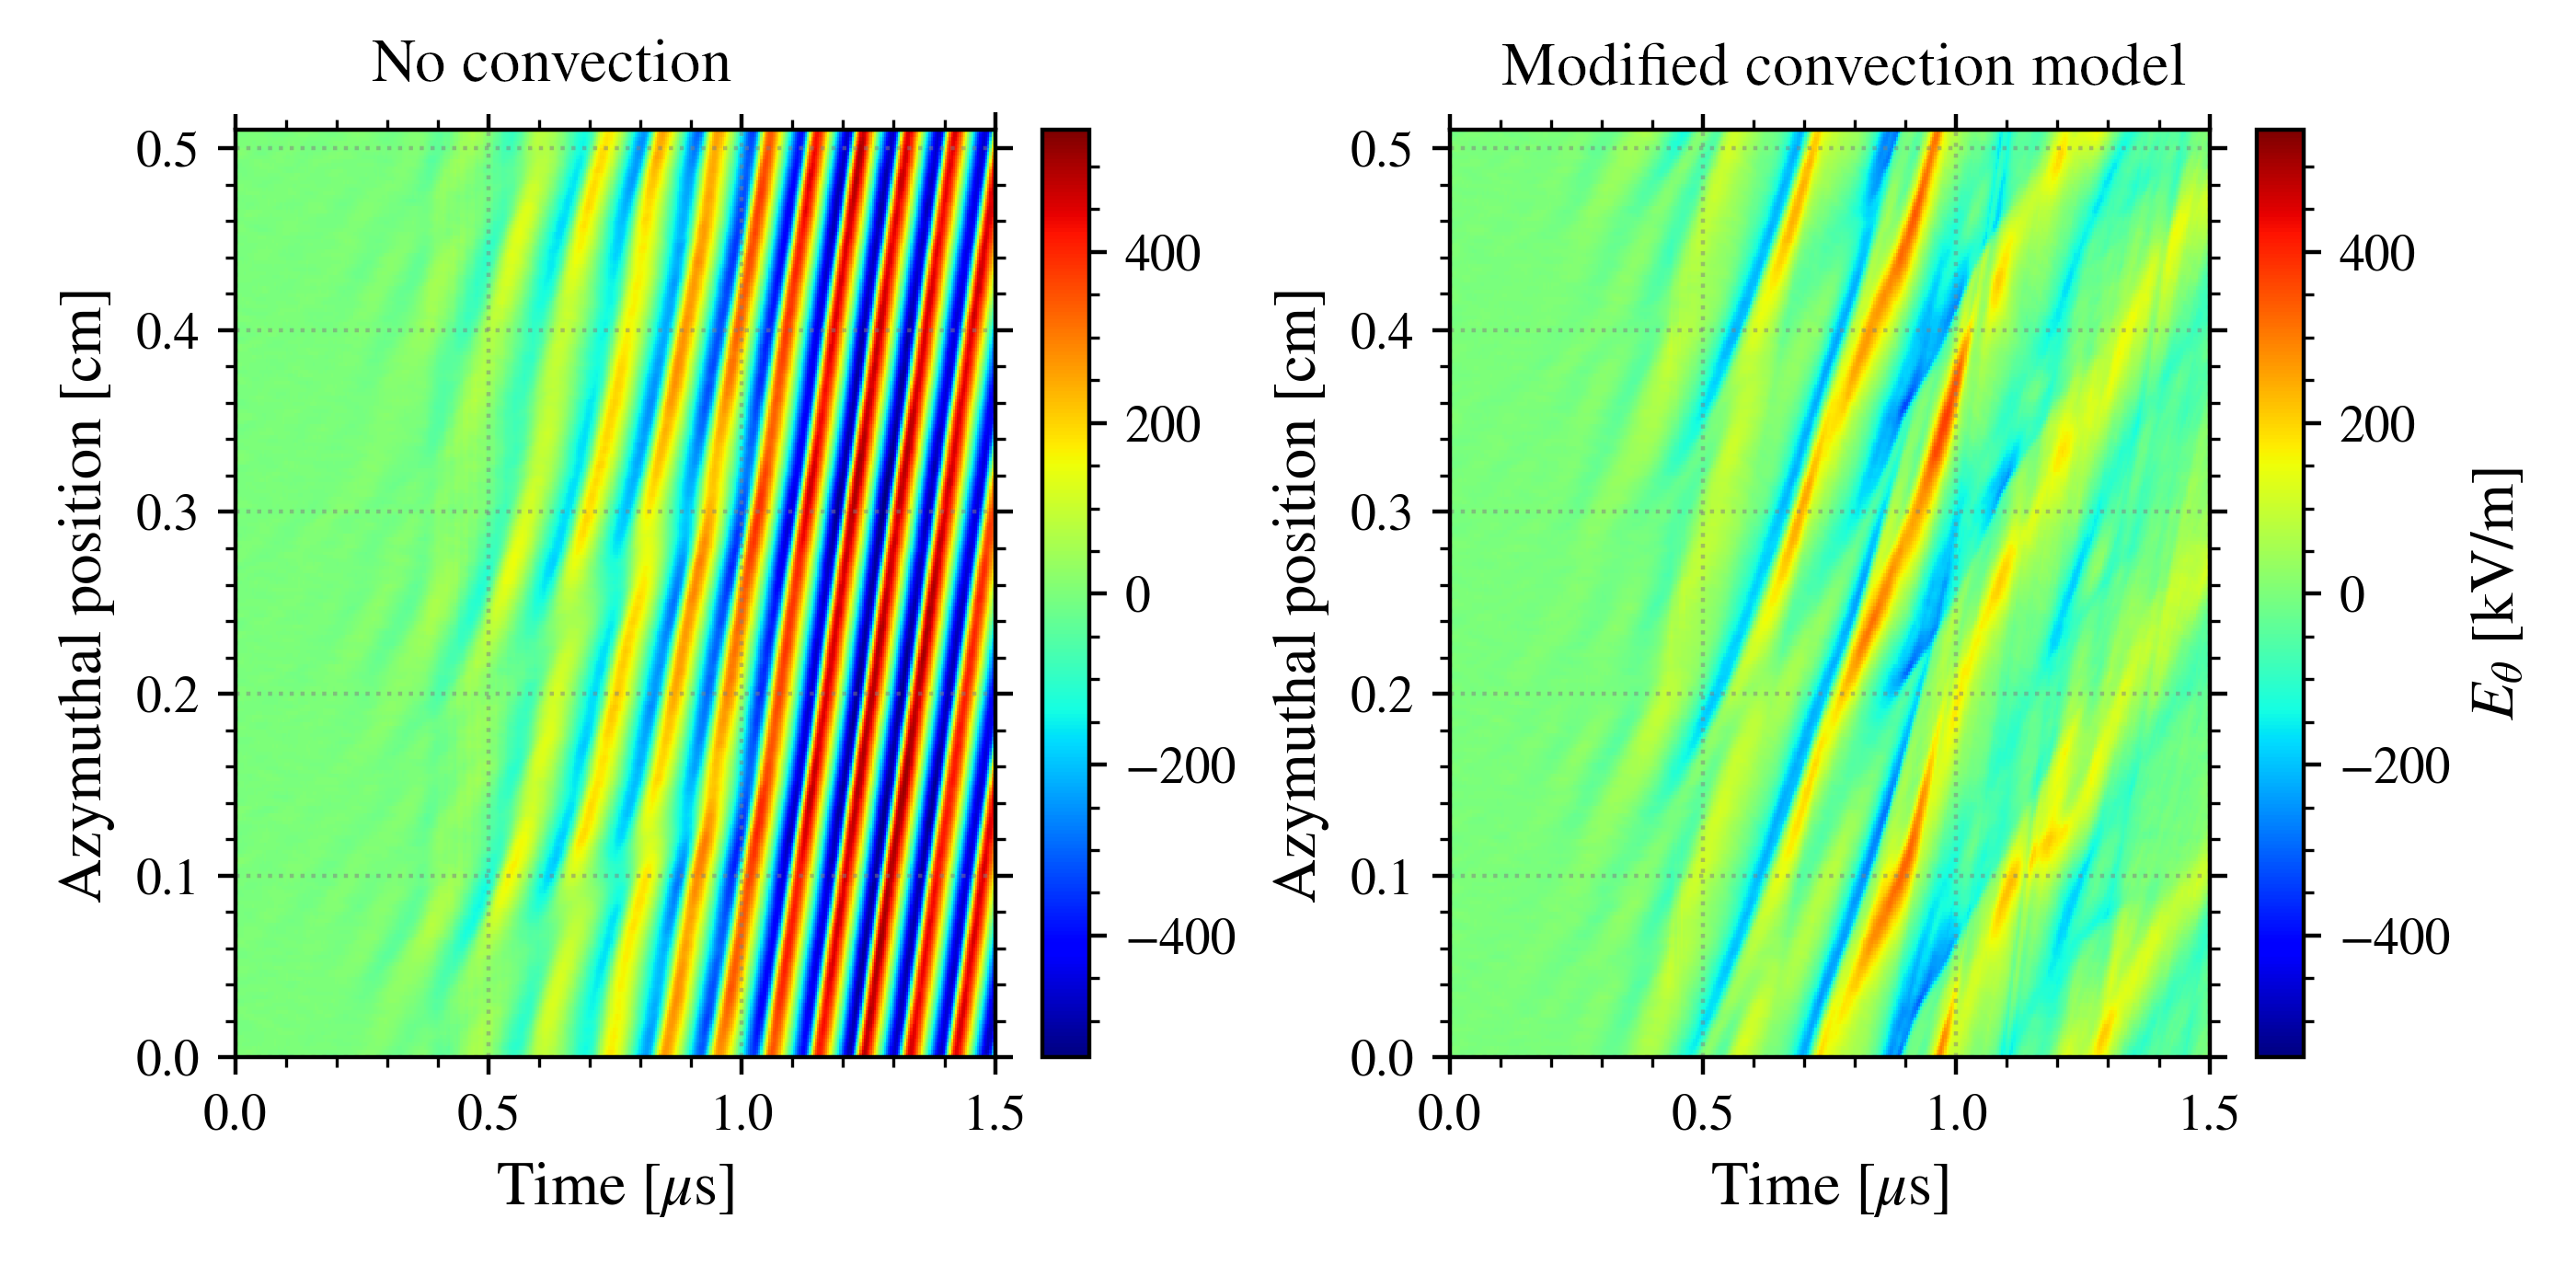
\includegraphics[width=\defaultwidth]{Compare_no_new_Reinj_Oz}
        \caption{Time evolution of the azimuthal electric field at the center of the radial dimension with and without the noiseless convection model. }
        \label{fig-newconv_noconv}
      \end{figure}
      
      \Cref{fig-oldeconv_newconv} shows the  time  evolution of the azimuthal electric field at the center of the radial dimension  with the convection modeled using Lafleur's model and the noiseless model with a small azimuthal length.
      We can see that the two models gives almost exactly the same results.
      
      \begin{figure}[hbtp]
        \centering
        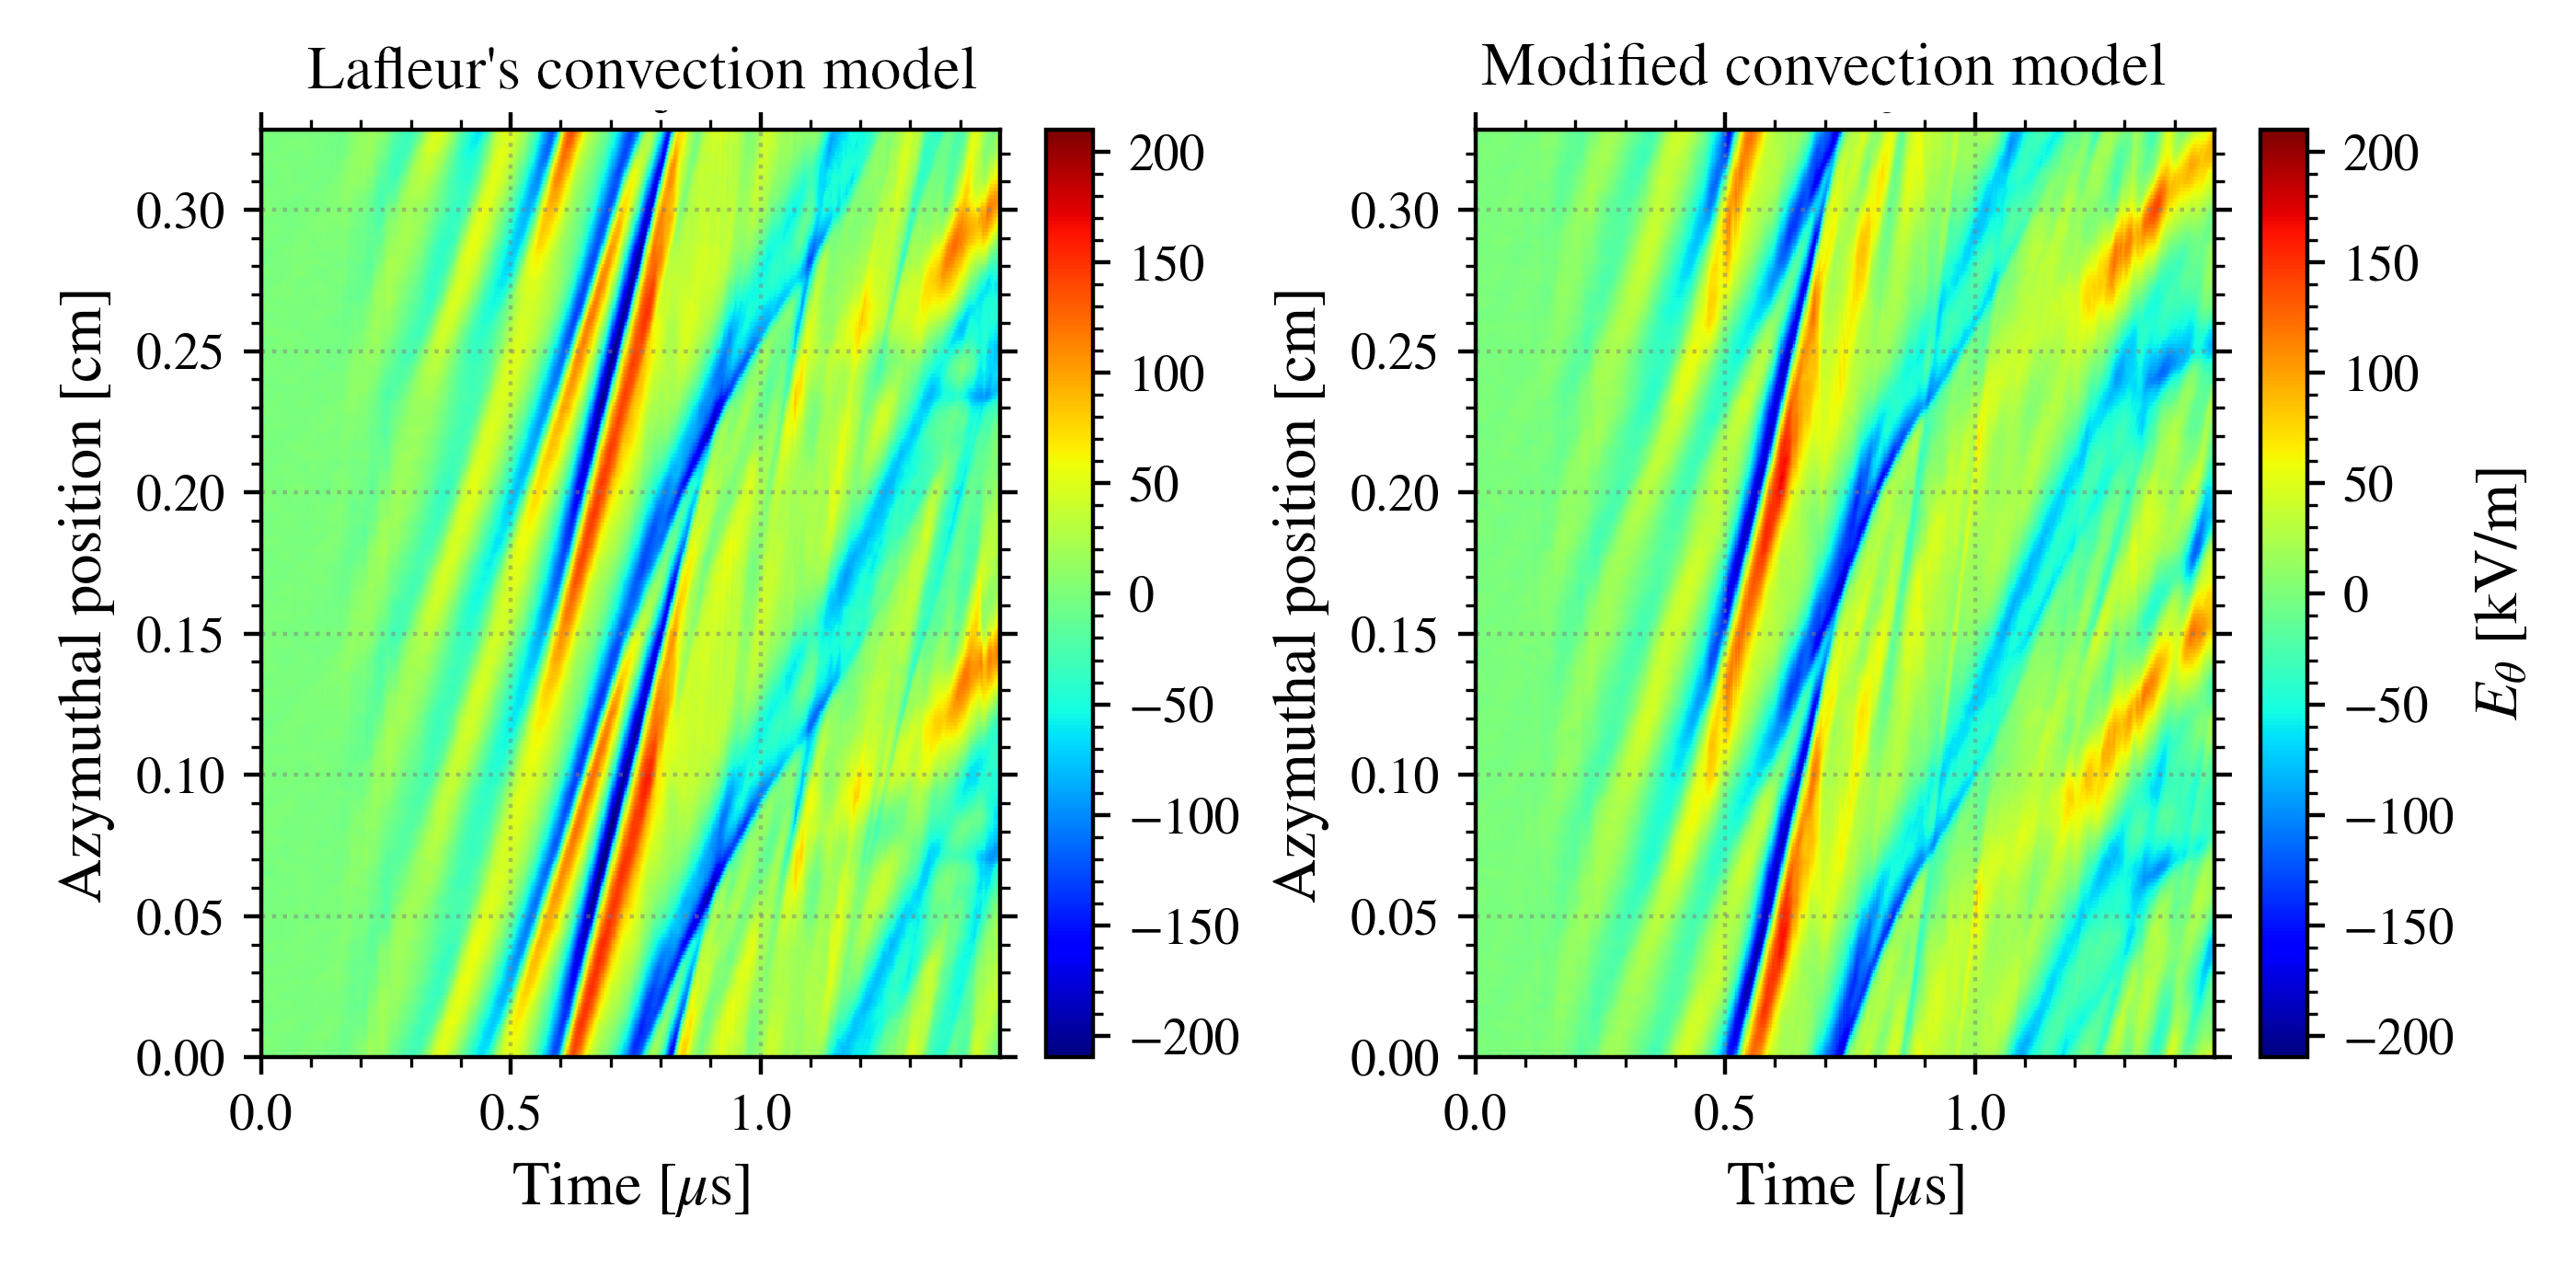
\includegraphics[width=\defaultwidth]{Compare_old_new_Reinj_Oz}
        \caption{Time evolution of the azimuthal electric field at the center of the radial dimension with the convection modeled using (left) Lafleur's model and (right) the noiseless model with a small azimuthal length.}
        \label{fig-oldeconv_newconv}
      \end{figure}
      
      
      \Cref{fig-oldeconv_newconv_longLZ} shows the  time  evolution of the azimuthal electric field at the center of the radial dimension  with the convection modeled using Lafleur's model and the noiseless model but using a longer azimuthal length than \cref{fig-oldeconv_newconv}.
      In this cases, we can see that Lafleur's convection model induces oscillations that are not observed with the noiseless model.
      
      \begin{figure}[hbtp]
        \centering
        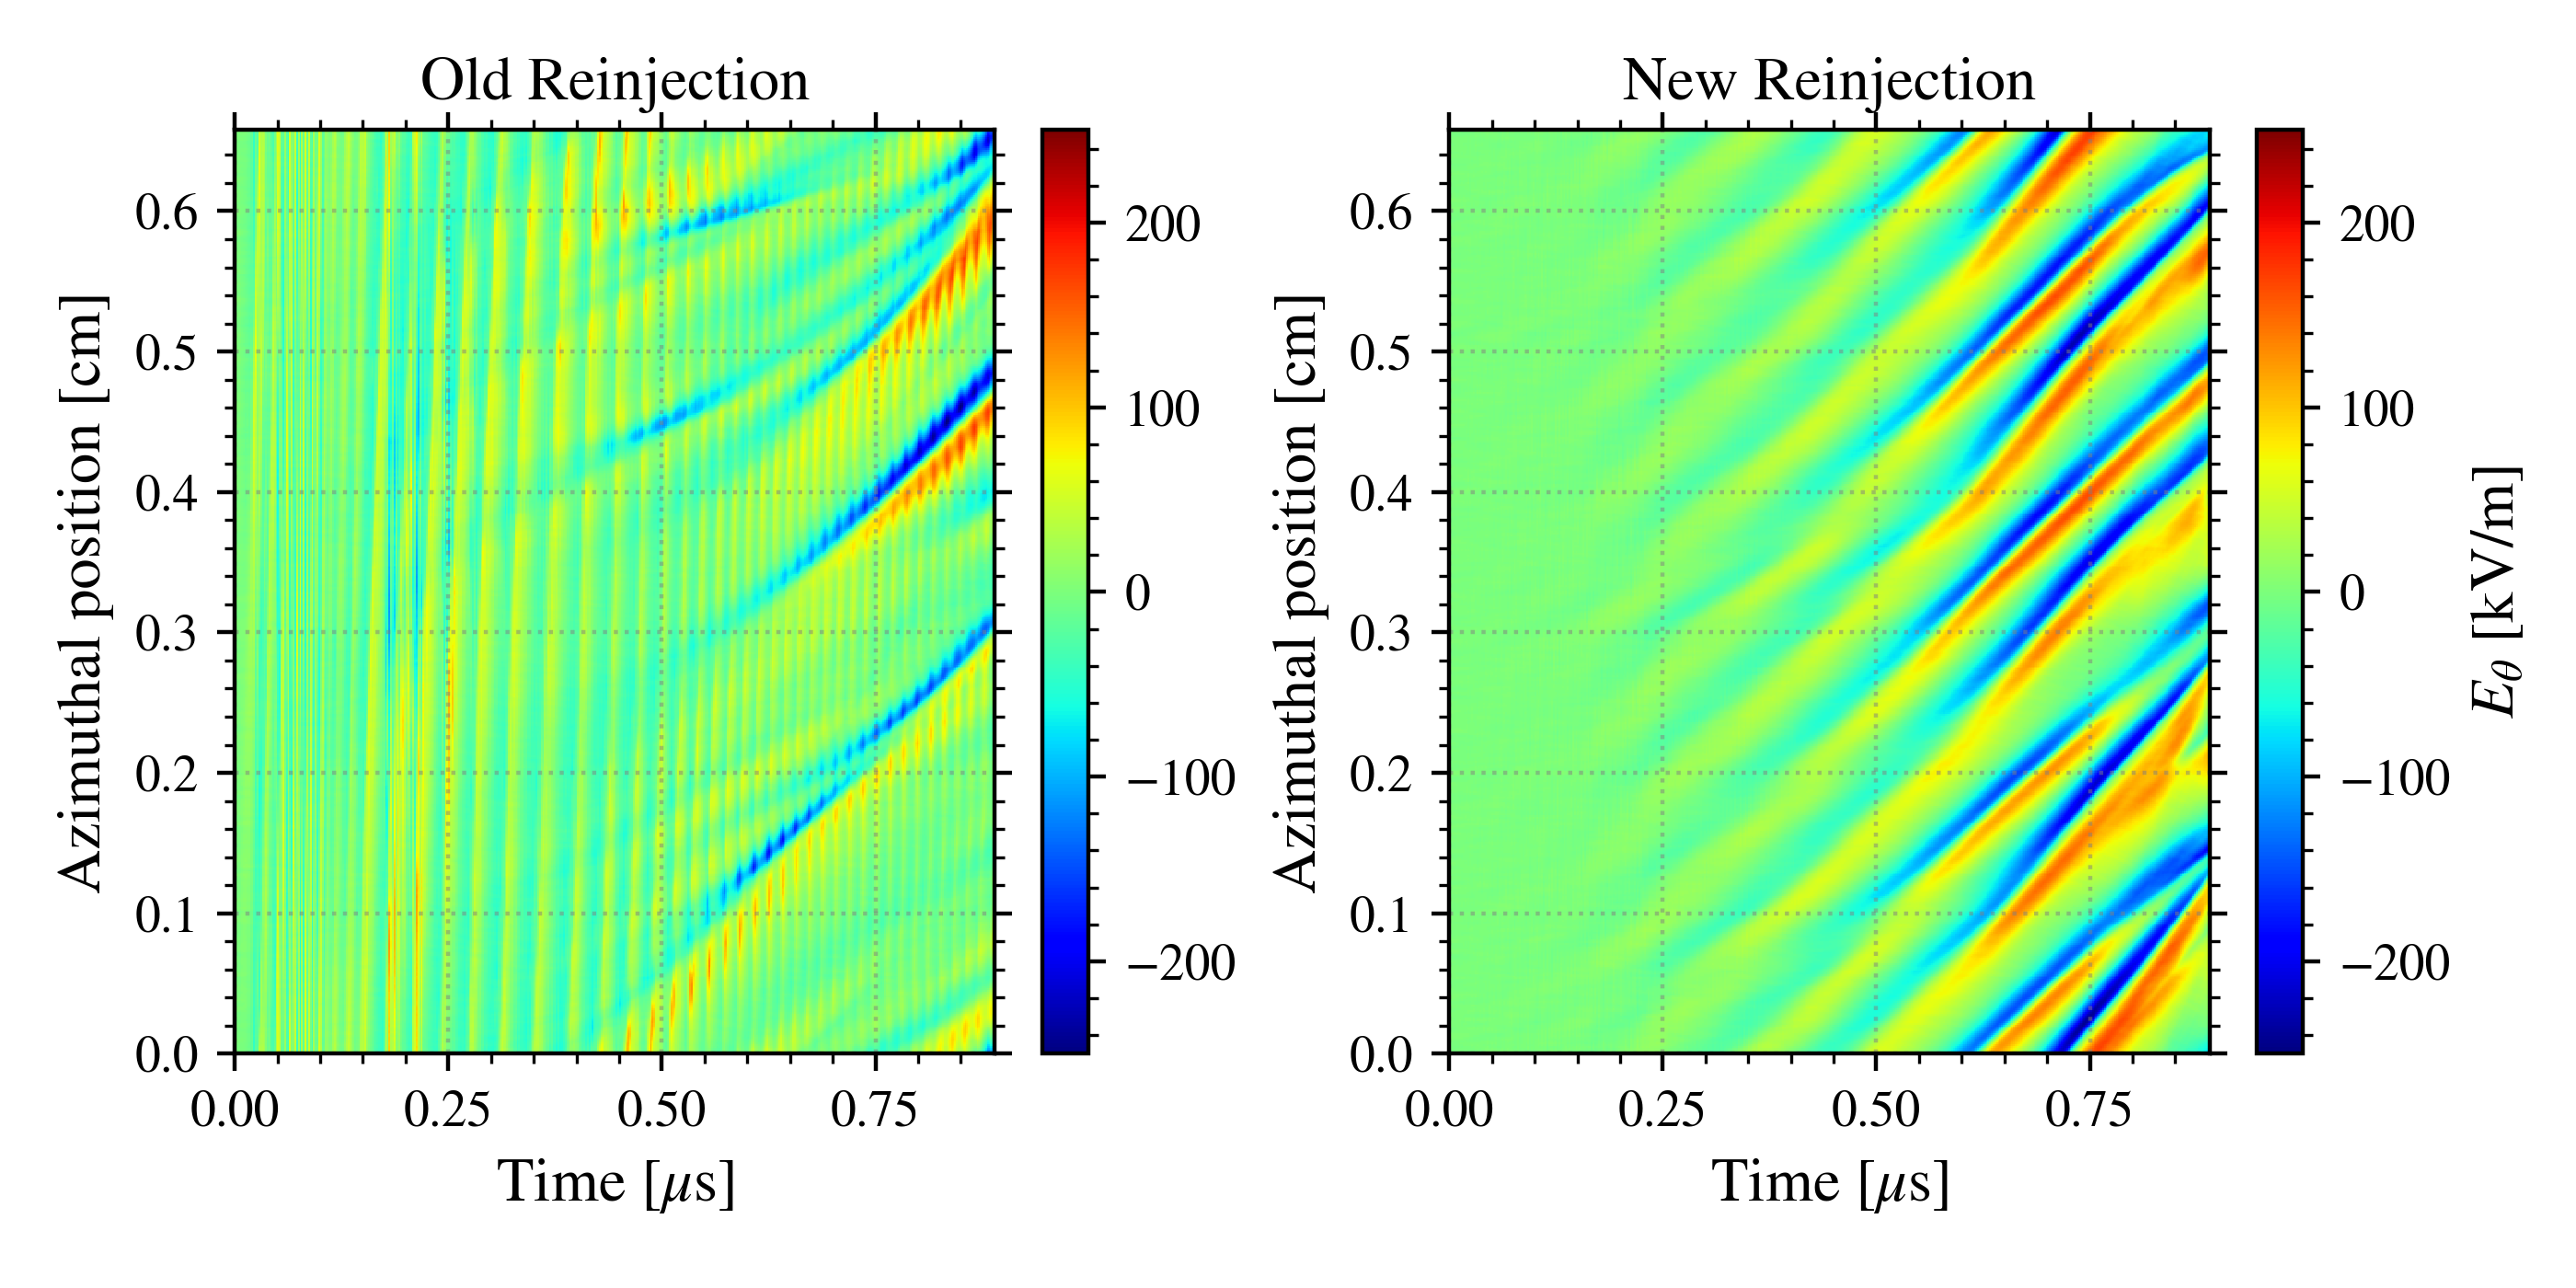
\includegraphics[width=\defaultwidth]{Compare_old_new_Reinj_Oz_LongLx}
        \caption{Time evolution of the azimuthal electric field at the center of the radial dimension with the convection modeled using (left) Lafleur's model and (right) the noiseless model with a longer azimuthal length.}
        \label{fig-oldeconv_newconv_longLZ}
      \end{figure}
      


      Theses observations have shown that Lafleur's convection model induces a noise on the charge density, that do not affect the simulation when the domain size is small, but can rise numerical artefacts when the domain size is larger.
      We have seen that the minor modification on the model do not affect the simulations results on a small domain, but allow us to use larger simulation domain without any numerical artefacts.
      
      Unfortunately, the new model has been developed during the last year of my theses.
      Hence, the first simulation results have been obtained using Lafleur's convection model.
      As seen in \cref{fig-oldeconv_newconv}, on a small geometry the results are not affected, hence there is no need to verify all of the simulations obtained.
      On the other hand, in order to study the instability, it is useful to have a longer azimuthal, in order to obtain a more resolved frequency spectra.
      Hence, the modified convection model  used in this case.
      \inlinenote{Give precise sections where it is used}
          
    \subsection{Effects on a \ac{2D} simulation domain}
      
      The mathematical development of \cref{sec-mathnoise} has been done in \ac{1D}.
      We can legitimately wonder is the results  can be extended directly to a \ac{2D} domain.
      A mathematical definition of $\aziE_{, 1}$ is more difficult, as we have, neglecting the dielectric layers,
      \begin{equation} \label{eq-aziE}
        \aziE_{, 1} = \partial_{\theta} \phi_1 \text{ such that } \grad \cdot \grad \phi_1 = - \frac { \N(0, \stdconv)}{\epsilon_0} \text{ following the \ac{BC}}.
      \end{equation}
      The \ac{BC}s are
      \begin{itemize}
        \item periodic \ac{BC} in the azimuthal direction,
        \item Dirichlet \ac{BC} in the radial direction, modeling grounded walls,
      \end{itemize}
      which translate as
      \begin{align}
        &\phi = 0 \text{ for } r=0 \text{ and } r=L_r, &\forall \theta \label{eq-BC1} \\
        &\phi(\theta = 0)= \phi(\theta = L_{\theta}) , &\forall r \label{eq-BC2}
      \end{align}
      
      Solving \cref{eq-aziE,eq-BC1,eq-BC2} analytically is much more difficult that the \ac{1D} development because of the Dirichlet \ac{BC}.
      \nomenclature[N]{Dirichlet Boundary condition\string:}{ a type of boundary conditions for which the field is fixed. For instance for grounded electrodes on the plasma potential\string: $\phi = 0$}
      However, we can investigate it numerically, by solving \cref{eq-aziE} for a given random source term.
      Using a Monte Carlo approach, the results are averaged 50 times in order to better observe the mean behaviour in respect to the noise (i.e. increasing signal to noise ratio).
        
      \Cref{fig-dftLr} shows the \ac{DFT} of the source term \[\rho_1 = \N(0, \stdconv),\] the resulting azimuthal electric field $\aziE_{, 1}$ and plasma potential $\phi$ computed on the centreline of the simulation domain in the radial direction, for three different radial length expressed in number of cell $N_x$.
      Is also showed the "equivalent" source term $\rho_{\rm eq}$, which is the source term that would give the frequency spectra of $\aziE_{, 1}$ observed in a \ac{1D} domain
      
      \begin{equation} \label{eq-equirho}
        \rho_{\rm eq} = \epsilon_0 \partial_\theta \aziE_{, 1}.
      \end{equation}
      The results are given for different radial length $N_x=15,50 \text{ and } 200$, while the azimuthally length $N_y=200$ is kept constant.
      We can see that the plasma potential and the electric field show larger amplitude for small wave numbers (large wavelength) compared to large wave numbers in the three cases.
      However, the amplitude of the smaller wave numbers is affected.
      In the cases of small radial length ($N_x=15 \text{ and } 50$), the spectra of the electric field is not monotonic.
      This can be explained by the Dirichlet \ac{BC}s that {\it pin down} the fluctuation of the plasma potential.
      
      However, even though the amplitude is reduces in \ac{2D} with small radial direction compared to a \ac{1D} model, we still observe large amplitude of small wave number oscillations in both the electric field and the plasma potential.
      Hence, the conclusions of  \cref{sec-mathnoise} derived in \ac{1D} can be legitimately used for \ac{2D} domains.
      
      
      
      \begin{figure}[hbtp]
        \centering
        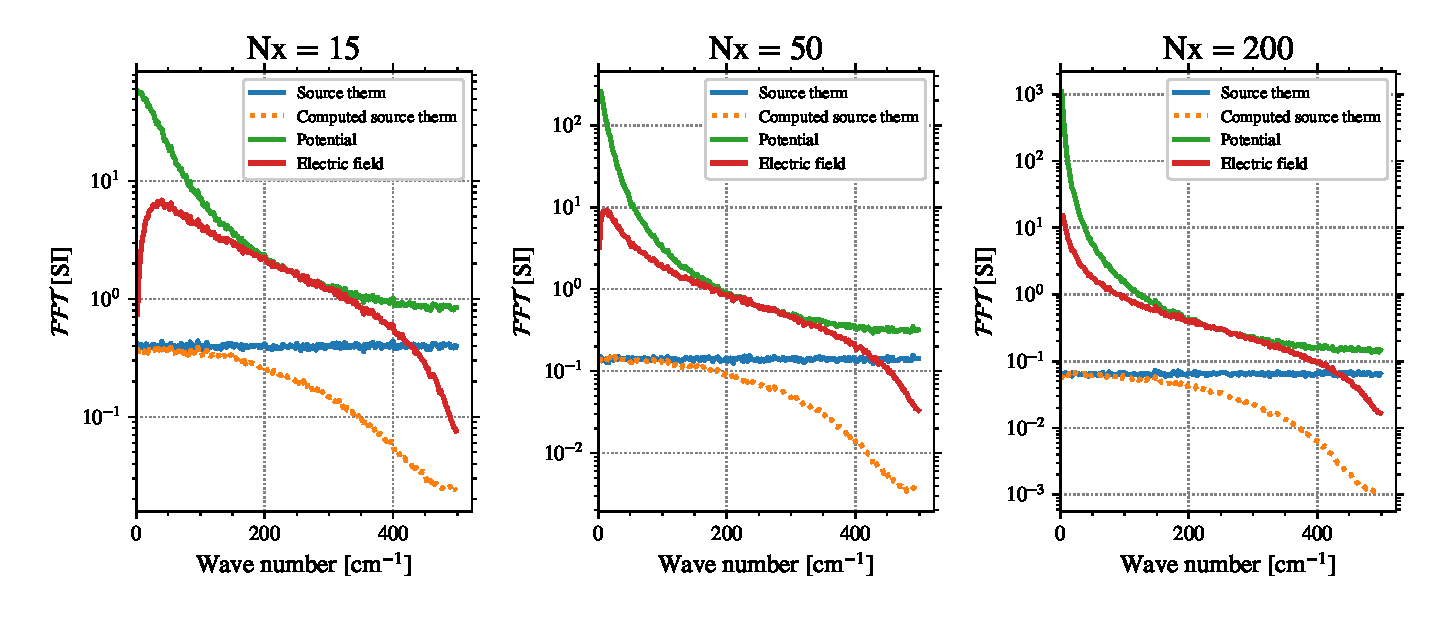
\includegraphics[width=\textwidth]{effect_Lr}
        \caption{\ac{DFT} of the source term $\rho_1 = \N(0, \stdconv)$, the resulting azimuthal electric field $\aziE_{, 1}$ and plasma potential $\rho$ computed on the centreline of a radial-azimuthal simulation, and the "equivalent" source term defined by \cref{eq-equirho}. $N_y=200$. }
        \label{fig-dftLr}
      \end{figure}
      
      






% !TEX root=/home/tavant/these/manuscript/src/manuscript.tex

\section{Secondary electron emission}
\label{sec-seemodel}
When an incident electron reaches the wall material, several scenarii are possible, as described in \citet{villemant2018}
\begin{enumerate}
  \item Elastic reflection\string: the electron encounters only elastic collision with the material, hence its energy is constant. However, its reflection is not necessary specular.
  \item Inelastic reflection\string: the electron looses some of its energy to the material before returning to the plasma.
  \item Secondary electron emission\string: the energy of the primary electron is enough to extract one or more electrons from the material.
  \item No emission, the electron is absorbed by the wall.
\end{enumerate}

The probability \proba{}  that one event happens instead of another depends predominantly on the particle energy, and weakly on its  impact angle.
Concerning the mean flux of electron incident and emitted, we uses the mean emission rate, or yield, \rate
\begin{equation*} \label{eq-ratedifinition}
  \rate = \frac{\Gamma_{e, \rm secondary}}{\Gamma_{e, \rm primary}}
\end{equation*}
which can be developed using the distribution function to 
\begin{equation*} \label{eq-ratedifinition_evdf}
  \rate = \frac{\iiint_{\Omega} v_x \proba(\vect{v_e}) f(\vect{v_e}) d^3v}{\iiint_{\Omega} v_x \proba(\vect{v_e}) f(\vect{v_e}) d^3v}
\end{equation*}
with $\Omega$ the ensemble of $\vect{v_e}$ directed toward the wall\string: $\vect{v_e} \cdot \vect{n} > 0$, with $\vect{n} $ the unit vector normal to and toward the wall.

\subsection{Models of emission } \label{subsec-seemodels}
Several models can be used to describe the electron emission.

\paragraph{Monte Carlo models} are the more realistic.
 They are based on the computation of the trajectory of the electrons through the material, during which the electron can encounter several interactions with the material.
 Each interactions can modify the electron direction, energy, and generate new electron.
 Several models have been proposed, as \citet{furman2002,pierron2017}.
 These models allow a precise characterization of the processes, but depends of a large number of parameters difficult to obtain due to the lack of experimental data.
 
\paragraph{Analytical models} provides a simplified description of the rate of emission.
Their complexity depends of the precision desired.
The most largely used are the models of \citet{vaughan1989,barral2003a,sydorenko2006b}.

In this work, we are interested only in representing qualitatively the electron emission.
Moreover, \citet{croes2017} showed that changing the model used do not affect significantly the results. 
Hence, we will use the model of \citet{barral2003a} for its simplicity.

\subsection{Barral electron emission model}
\label{sec-modelused}

The emission model used follows a linear-saturated law for the probability of emission with three parameters. 
It describes the total emission corresponding to the sum of the elastic and inelastic backscattering and the secondary electron emission.
\begin{equation} \label{eq-proba_barral}
  \proba(\ek) = 
  \begin{cases}
    \proba_0 + (1 - \proba_0) \frac{\ek}{\crover}   &\text{ if } \ek <  \ek_{\max} \\
    \probamax &\text{ if } \ek \geq \ek_{\max}
  \end{cases}
\end{equation}
where $\ek$ is the kinetic energy of the incoming electron, $\proba_0$ is the asymptotic probability of emission at energy null, $\crover$ is the crossover energy above which the probability of emission is higher that one, \probamax is the maximum probability and $\ek_{\max}= \frac{\probamax - \proba_0}{1 - \proba_0} \crover $ is the minimum energy for which $\rate = \probamax$ .
\Cref{eq-proba_barral} is illustrated in \Cref{fig-modelbarral}.

\begin{figure}[hbtp]
  \centering
  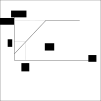
\includegraphics[width=\defaultwidth]{barral}
  \caption{Linear-saturated emission model from \citet{barral2003a}.}
  \label{fig-modelbarral}
\end{figure}

 We suppose that all of the electrons emitted are isotropically emitted following a Maxwellian flux distribution function of temperature $\Tsee$.
 The parameters $\proba_0$,  $\probamax$ and $\crover$ can be obtained from experiments. 
 \Cref{tab-seeparames} shows the crossover energy and the  probability of emission at energy null for different materials.
 The value of $\proba_0$ is always close to $0.5$, but $\crover$ can vary from 18 to 305 V.
 Hence, in the following parametric studies, $\proba_0$ will be kept at 0.5 while we vary $\crover$ from low values, corresponding to highly emmissive materials, to high values, representing less emmissive materials.
 
 \begin{table}[hbtp]
   \ra{1.3}
   \centering
   \caption{Emission parameters for different materials, from \citet{barral2003a}.}
   \label{tab-seeparames}
   \begin{tabular}{@{}lll@{}} \toprule
   Material & $\crover$ (V)& $\proba_0$ \\ \midrule
   BN-SiO$_2$ & 53 & 0.45 \\ 
   Al$_2$O$_3$ & 18  & 0.57 \\ 
   SiC     &  43  &0.69  \\
   Graphite & 305  & 0.40 \\ 
   \bottomrule
   \end{tabular}
 \end{table}
 

% !TEX root=/home/tavant/these/manuscript/src/manuscript.tex

\section{Electron cross-field transport}
  \label{sec-transport}
  
  The electron mobility in the axial direction $\mobe$ is defined as the ratio between the mean velocity $u$ and the electric field
  \begin{equation} \label{eq-mudef}
    \mobe = \frac{u_{e,z}}{E_z}
  \end{equation}
  with $u_{e,z}=<v_{e,z}>$ the electron mean velocity
  \nomenclature[Q]{\ensuremath{ u_{e,z}}}{Electron mean velocity int he axial direction : $u_{e,z} = < v_{e,z}>$}
  In the \ac{PIC} simulations, \cref{eq-mudef} can be used directed to compute $\mobpic$.
  
  In the classical drift diffusion theory of the electron mobility transverse to a magnetic field, the mobility is due to collisions as \citep{chen2006,meezan2001}
  \begin{equation} \label{eq-mobclas}
    \mobcla = \frac{e}{m_e} \frac{\nu_m}{\nu_m^2 + \oce^2}
  \end{equation}
  with $\oce=\frac{e B}{m_e}$ the electron cyclotron frequency and $\nu_m$ the electron-neutral momentum transfer collision frequency.
  \nomenclature[Q]{\ensuremath{ \oce}}{ Electron cyclotron frequency $\oce=\frac{e B}{m_e}$}
  \nomenclature[Q]{\ensuremath{ \nu_m}}{  electron-neutral momentum transfer collision frequency}
  
  At the exit plan, the classical mobility predict a mobility of the order of $\mobcla=0.001 -- 0.01\mobunit$ \citep{adam2008a}.
  
  The kinetic approach allowed \citet{lafleur2016a} to propose a modified mobility due to the oscillations of the electron density and the azimuthal electric field of the \ac{ECDI}.
  This effective mobility obtained is 
  \begin{equation} \label{eq-defmobeff}
    \mobeff = \mobcla \lp 1 - \frac{\oce}{\nu_m}  \frac{< \dne \dEt >_{\theta} }{n_0 E_z}   \rp
  \end{equation}
  with \dne and \dEt the fluctuations in the azimuthal directions of the electron density and azimuthal electric field, respectively, the operator $< . >_{\theta}$ is the average in the azimuthal direction, and $n_0$ is the average plasma density.
  In the case where $\nu_m << \oce$, \cref{eq-defmobeff} can be simplified to 
  \begin{align} 
    \mobeff &= \frac{\frac{e}{m_e} \nu_m}{\oce^2} \lp 1 - \frac{\oce^2}{\nu_m}  \frac{< \dne \dEt >_{\theta} }{n_0 E_z}   \rp \nonumber \\
    &= \frac{< \dne \dEt >_{\theta} }{n_0 E_z}   \frac{1}{B_r} \label{eq-mobeffsimple}
  \end{align}
  which shows that the instability enhances the electron axial mobility in a wave similar to an $E \times B$ drift.
  The electric field $E_{\theta}$ oscillates and presents a zero mean value, but the average effect on the electron transport is not zero if the correction between \dEt and \dne is not zero.
  
  In  \citet{lafleur2016a}, the authors present the instability effect as an electron-ion friction force $\Rei = - e < \dne \dEt >_{\theta}$.
  Under the assumption that the saturation of the instability is mainly due to ion trapping, the electron-ion friction force can be simplified to
  \begin{equation} \label{eq-rei-sat}
    \Rei^{sat} = \frac{e \norm{\grad \cdot (n_e \Te \vect{v_i})}}{4 \sqrt{6} c_s} \simeq \frac{e n_e \Te \viout}{4 \sqrt 6 c_s L_z}
  \end{equation} 
  \nomenclature[Q]{\ensuremath{ \vect{v_i}}}{  ion velocity vector}
  \nomenclature[Q]{\ensuremath{ c_s}}{ ion sound speed $c_s=(e \Te/m_i)^{1/2}$ }
  where $\vect{v_i}$ is the ion velocity, $c_s=(e \Te/m_i)^{1/2}$  is the ion sound speed, and the spatial derivative in has been approximated across the axial simulation direction, with $\viout$ the ion outlet velocity 
  \begin{equation} \label{eq-viz}
    \viout = \sqrt{\frac{2 e U_z}{m_i}},
  \end{equation}
  with $U_z = E_z L_z$ the total potential difference in the axial direction.
  \nomenclature[Q]{\ensuremath{ U_z}}{   total potential difference in the axial direction $U_z = E_z L_z$}
  
  Using \cref{eq-rei-sat} in \cref{eq-mobeffsimple}, we obtain the simplified expression
  \begin{equation} \label{eq-mobeffsat}
    \mobeffsat = \frac{\sqrt{\frac{\Te}{U_z}}}{4\sqrt{3}B_r}.
  \end{equation}
  
  \Cref{eq-mobeffsat} shows that for the radial and azimuthal \ac{2D} geometry being used here, the enhanced mobility due to \ac{ECDI} scales as the square-root of the electron temperature $\Te$ if the simulation parameters are constant.
  However, it is not the case in general, as the saturation of the instability can be also due to convection, and there are axial gradients in the electron temperature and plasma density as well.
  
  We can note that $\mobpic, \mobeff$ and $\mobcla$ are defined at every position of the simulation, but that $\mobeffsat$ can only be globally calculated. 
  
  
  
  
  
% !TEX root=/home/tavant/these/manuscript/src/manuscript.tex

\section{Sheath model with electron emission}
  \label{sec-sheath}
  
  \inlinenote{Ici, le model est introduit rapidement... Peut-etre le faire plus explicitement a partire des equations fluid ?}
  
  The sheath model featuring SEE processes has been historically studied by Hobbs and Wesson \citet{hobbs1967}, but is still an active research topic nowadays \citep{ahedo2005}.
  The sheath is often considered to be collision-less and isothermal, while the plasma is composed of hot Maxwellian electrons and cold ions. A third population of electron-induced secondary electrons is also present in the sheath, and the re-emission rate $\rate$ is assumed to be constant.
  The SEE process modifies the potential drop in the sheath as \citep{hobbs1967}
  \begin{equation} \label{eq-sheathhobbs}
    \dphisheath = \Tepar \ln \lp (1 - \rate) \sqrt{\frac{m_i}{2 \pi m_e}}   \rp
  \end{equation}
  with $\Tepar$ the electron temperature in the direction parallel to the magnetic field, thus normal to the walls.
  Adding a pre-sheath drop of $\Tepar/2$ \citep{ahedo2002}, the total potential drop to the wall becomes
  
  \begin{equation} \label{eq-total_drop}
    \dphi = \dphisheath + \frac{\Tepar}{2} =  \Tepar \lp \frac{1}{2} + \ln \lb (1 - \rate) \sqrt{\frac{m_i}{2 \pi m_e}}   \rb  \rp
  \end{equation}
  
  In \Cref{eq-sheathhobbs,eq-total_drop}, we uses $\Tepar$ as in general, and more precisely for low-pressure magnetized plasma, the electrons can be anisotrope.
  
  We can see that \cref{eq-sheathhobbs} becomes negative for a critical value of the emission rate
  \begin{equation} \label{eq-ratecrone}
    \rate_{\rm max} = 1 - \sqrt{\frac{2 \pi m_e}{m_i}} \simeq 0.985 \text{ for Xenon.}
  \end{equation}
  
  However, before that $\rate$ attains $\rate_{\rm max}$, the model of \citet{hobbs1967} presents another behaviour against the hypotheses of  \cref{eq-sheathhobbs}, as the sheath becomes \ac{SCL}.
  In the \ac{SCL} conditions, the electron emission is so large that the electric field at the wall becomes zero 
  \begin{equation} \label{eq-scl_Er}
    \deriv{\phi}{r} \at{\rm wall}= 0 
  \end{equation}
  In this case, the plasma potential drop to the wall for any ion mass is \citep{hobbs1967}
  \begin{equation} \label{eq-dphi_scl}
    \dphiscl \simeq 1.02 \Tepar,
  \end{equation}
  and the limit emission rate is
  \begin{equation} \label{eq-ratecr}
    \ratecr \simeq 1 - 8.3 \sqrt{\frac{m_e}{m_i}}
  \end{equation}

  For xenon, \cref{eq-ratecr} gives $\ratecr = 0.983$ \citep{goebel2008}.\footnote{This value of 0.983 is obtained after several approximation, as \cref{eq-scl_Er} , some of which should not allow to use three significant digits. That's why it does not exactly match with the numerical results presented in \cref{fig-potential_profile}.}

  \Cref{fig-potential_profile} illustrates the sheath model of \citet{hobbs1967} by showing the plasma potential profile in the sheath for different values of electron emission rate for a xenon plasma.
  \cref{fig-potential_profile}.{\bf a} gives the potential $\phi$ normalized by $\dphisheath$ from \cref{eq-sheathhobbs}, and \cref{fig-potential_profile}.{\bf b} gives $\phi$ not normalized.
  We can see in \cref{fig-potential_profile}  that for $\rate < \ratecr$, the plasma potential reached $\dphisheath$.
  However, for $\rate > \ratecr$, the plasma potential do not reaches $\dphisheath$, resulting in a non-zero current to the wall.
  Indeed, the sheath is not monotonic in this case, hence the hypotheses needed to develop \cref{eq-sheathhobbs} are not fulfilled.
  
  In \cref{fig-potential_profile}.{\bf b}, we can see that at $\rate \simeq \ratecr$, the plasma potential tends towards $\Te$, as mentioned by \cref{eq-dphi_scl}.
  \begin{figure}[hbtp]
    \centering
    \begin{tabular}{c c}
      \subfigure{plasma_profile_normed}{a}{25,20} & 
      \subfigure{plasma_profile}{b}{25,20} 
    \end{tabular}
    \caption{Evolution of the plasma potential in the sheath for different values of electron emission rate $\rate$ fro a xenon plasma, ({\bf a}) normalized by the total potential drop $\dphisheath$ from \cref{eq-sheathhobbs}, and ({\bf b}) normalized by the electron temperature, but $\dphisheath/\Te$ is noted with the black dotted line.  }
    \label{fig-potential_profile}
  \end{figure}
  
  
% !TEX root=/home/tavant/these/manuscript/src/manuscript.tex



\section{Conclusion}
  \label{sec-conclusion_ch1}
  

  In order to study the plasma wall interaction in an \ac{HET}, we developed a bi-dimensional simulation code using \ac{PIC}-\ac{MCC} modeling.
  As the electrons drift azimuthally due to the $E \times B$ configuration, the \ac{ECDI} rises, enhancing the cross field transport of the electron toward the anode.
  The walls closing the chamber in the radial direction are also important for the discharge behaviour.
  Hence, in order to compare the interaction between these phenomena, we simulate the radial-azimuthal domain.
  
  A special care have been taken during the developement of \LPPic, the \ac{2D}-\ac{3V} \ac{PIC}-\ac{MCC} simulation code, concerning
  \begin{itemize}
    \item the modeling of the axial convection, in order to model the energy losses and so attain a steady state,
    \item the modeling of the radial boundary with the dielectric layer included in the simulation domain.
  \end{itemize}
  
  Several theories have also been given in order to better understand the \ac{PIC} simulation results, especially concerning the electron cross-field mobility and the sheath model in presence of electron emission.

% \acresetall
% !TEX root=/home/tavant/these/manuscript/src/manuscript.tex




\chapter{Parametric study of the dielectric characteristics}
\label{ch-2}
\headerchaptername{Dielectric parametric study}

\begin{Chabstract}
We use the PIC simulation code described in \cref{ch-1} to perform a parametric study over the two aspects of the dielectric walls\string: the secondary electron emission, and the modification of the electrostatic boundary condition.
We observe their impacts on the electron cross-field mobility, the electron mean temperature and the sheath characteristics.
The electrostatic boundary condition does not modify the results significantly.
On the other hand, the electron emission increases the near-wall mobility while decreasing the mean electron temperature, that reduces the importance of the \ac{ECDI} on the mobility.
A large discrepancy is observed between the sheath model of \cref{sec-sheath} and the PIC simulation results.
\end{Chabstract}



\minitoc


% 
% Structure \string:
% 
% {\bf II. Parametric study of the dielectric} 30 pages
% \begin{zzz}
%   This chapter takes the 1rst paper which uses Vivien's results.
% 
%   2.1 Fully metallic wall (no SEE, grounded).
% 
%   2.2 Impact of Dielectric layer without SEE
% 
%   2.3 Impact of SEE with grounded wall
% 
%   2.4 SEE and dielectric in the same time
% 
%   2.5 Discrepancy between $\mean{\Te}$, $\sigma_{PIC}$ and $\sigma_{theo} = \sigma_0 + (1 - \sigma_0) \frac{2 T_e}{\epsilon_0}$
% \end{zzz}


% !TEX root=/home/tavant/these/manuscript/src/manuscript.tex

\section{Simulation parameters}
  \label{sec-params}
  
  The simulation domain corresponds to the exit plane of the thruster.
  Hence, a neutral pressure $P_n$ of 0.1~mTorr and a plasma density $n_e$ of $\sn{1}{17}$ m$^{-3}$ are used.
  The fixed axial electric field and radial magnetic field are $E_z=\sn{2}{4}\,\volt\per\meter$ s and $B_r=200$ G, respectively.
  The rectangular \ac{2D} domain measures $L_r=2$~cm in the radial dimension and $L_{\theta}=0.5$~cm in the azimuthal direction.
  The axial length used for the convection is fixed at $L_z=1$~cm.
  It is important to note that the results shown in this chapter have been obtained at the beginning of my thesis, before the study of the convection presented in \cref{ch-1}.
  Hence, in this chapter we use the convection model of \citet{lafleur2016a}.
  However, we have validated at posteriori that the convection model used does not modify the results under the conditions studied.
  
  The numerical parameters are chosen to respect the stability criterion of \ac{PIC} simulation, and are presented in \Cref{parameters}
  
  \begin{table}[htbp] %PIC parameters
       \centering
       \ra{1.3}
       \caption{\label{parameters} Standard operating and numerical parameters used in the 2D PIC simulations of an HET.  The simulation results are given as representative values.}
       \begin{tabular}{@{}r c c c@{}} 
          \toprule
          {\bf Physical Parameter} & notation & Value & Unit \\
          \midrule
          Gas & & Xenon & - \\
          Domain dimensions & $L_{x} \times L_{y} \times L_{z}$ & $2.0 \times 0.5 \times 1.0$ & [cm$^3$] \\
          Radial magnetic field & $B_{0}$                    & $200$                 & [{G}] \\
          Axial electric field & $E_{0}$                    & $2 \times 10^{4}$     & [{Vm}$^{-1}$] \\
          Mean plasma density & $n_{0}$                    & $3 \times 10^{17}$    & [{m}$^{-3}$] \\
          Initial electron temperature & $\Te_{,0}  $               & $5.0$                 & [{V}] \\
          Initial ion temperature & $T_{i,0}   $               & $0.1$                 & [{V}] \\
          Secondary electron temperature & $T_{see}   $               & $1.0$                 & [{V}] \\
          Neutral gas pressure & $P_{n}     $               & $1.0$                 & [{mTorr}] \\
          Neutral gas temperature & $T_{n}     $               & $300$                 & [{K}] \\
          Neutral gas density & $n_{g}     $               & $3.22 \times 10^{19}$ & [{m}$^{-3}$]\\
          \midrule
          {\bf Simulation Parameter} &  &   &  \\
          
          Time step & $\Delta t  $                      & $4 \times 10^{-12}$ & [{s}] \\
          Cell size & $\Delta x = \Delta y = \Delta z $ & $2 \times 10^{-5}$  & [{m}] \\
          Number of particles per cell & $N/NG      $                      & $80$                & [{part/cell}] \\
          \midrule
          {\bf Typical quantities} &  &  &  \\ 
          Electron plasma frequency & $\omega_{pe}$               & $3.1 \times 10^{10} $  & [rad/s]\\
          Iopn plasma frequency & $\omega_{pi}$               & $36 \times 10^{6} $  & [rad/s]\\
          Electron cyclotron frequency & $\omega_{ce}$               &  $3.5\times 10^{9}$  & [rad/s] \\
          Electron Larmor radius & $r_{Le}$                    & 6$\times 10^{-4}$    & [m] \\
          \bottomrule
       \end{tabular}
    \end{table}
  
  
  The simulation is initialized with a uniform density of particles, following a Maxwellian distribution for temperature $\Te_{,0}$ and $\Ti_{,0}$ for the electrons and the ions respectively.
  
  
% !TEX root=/home/tavant/these/manuscript/src/manuscript.tex

\section{The base case}
  \label{sec-canonical}
  
  
  The {\it base} case corresponds to the case when the walls are grounded, and are fully absorbing. 
  It is the reference case that will be extensively described and commented.
  Then, it will be used as reference to analyze and quantify the effects of two characteristics of the dielectric walls on the studied discharges : the secondary electron emission, and the modification of the electrostatic boundary condition.
  
  \subsection{Initial phase of the simulation\string: \texorpdfstring{$t < 2\,\micro\second$}{ t < 2 microseconds} } \label{subsec-initlaphase}
  
  The initial phase of the simulation corresponds to the growth of the \ac{ECDI}, and the formation of the sheaths.
  Because of the growth of the instability, the electron transport increases as well, which increases the electron heating.
  The time scale of the sheath formation is governed by the ion inertia.
  It is roughly the same time scale as the saturation of the instability due to ion-trapping.
  
  \begin{figure}[hbt]
    \centering
    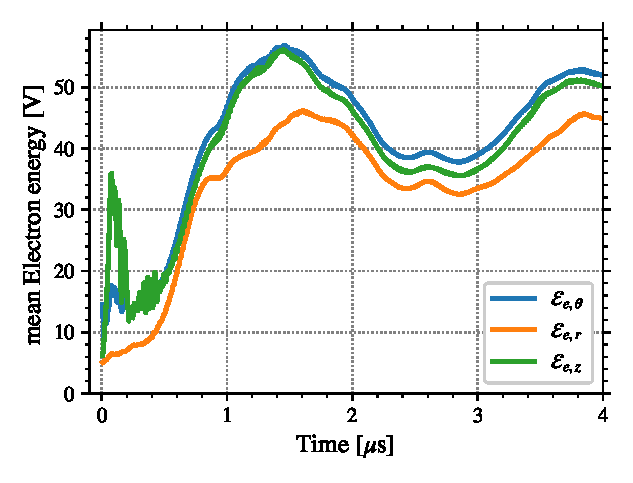
\includegraphics[width=\defaultwidth]{canonical_Te_start_directions}
    \caption{Temporal evolution of the electron mean kinetic energy decomposed over the three directions. Only the beginning of the simulation is shown.}
    \label{fig-canon_Te_strat}
  \end{figure}
  
  \Cref{fig-canon_Te_strat} shows the temporal evolution of the electron mean kinetic energy decomposed over the three directions, $\Ee_r, \Ee_{\theta}, \Ee_z$, such that
  \begin{equation} \label{eq-Ee_direction}
    \Ee_d = \frac{1}{n} \frac{1}{2} m_e \iiint_{\vect{v}}  v_{e,d}^2 f (\vect{v}) d^3v, \text{ with } d \in \{r, \theta, z  \}
  \end{equation}
  The mean kinetic energy is the sum of the thermal energy and the kinetic energy of the mean velocity.
  Because the electrons drift mainly in the azimuthal direction, we have
  \begin{equation} \label{eq-kinetic}
    \begin{cases}
      \Ee_r \simeq \frac{\Te_r}{2} \\
      \Ee_z \simeq \frac{\Te_z}{2} \\
      \Ee_{\theta} \simeq \frac{\Te_{\theta}}{2} + \frac{m_e}{2} \lp \frac{E_0}{B_0} \rp^2 \\
    \end{cases}
  \end{equation} 
  with $\frac{m_e}{2} \lp \frac{E_0}{B_0} \rp^2 \simeq  2.84\,\volt $.
  \nomenclature[Q]{\ensuremath{ \Ee}}{ Electron total kinetic energy, imposed of the thermal (or internal) energy and the kinetic energy of the mean velocity.  }
  We see that after some high frequency oscillations of $\Ee_{\theta}$ and $\Ee_z$ due to the cyclotron motion, the energies rise before stabilizing at $\Ee \simeq 45$V.
  The radial kinetic energy $\Ee_r$ is less than $\Ee_z$ and $\Ee_{\theta}$, but only by a small difference of $5\,\volt$, corresponding to roughly $10\%$.
  The small difference between the azimuthal and the axial kinetic energy is of the order of $2\,\volt$, as expected from the cyclotron motion of the electrons and \cref{eq-kinetic}.
  This means that the electrons are almost isotropic.
  
  
  \begin{figure}[hbt]
    \centering
    \begin{tabular}{@{} c c}
      \subfigure{time_r_mean_n}{a}{20, 20} &
          
      \subfigure{time_r_mean_phi}{b}{20, 20} 
    \end{tabular}
    \caption{Temporal evolution of the radial profile of the ({\bf a}) electron density and ({\bf b}) the plasma potential averaged azimuthally.}
    \label{fig-tx_n_phi}
  \end{figure}

  We can see in \Cref{fig-tx_n_phi} the evolution of the radial profile of the electron density on the plasma potential over the same period as \cref{fig-canon_Te_strat}.
  We observe on both quantities the formation of the sheath and the evolution toward a steady-state.
  
  \subsection{Saturated quasi steady-state\string: \texorpdfstring{$t \geq 2\,\micro\second$}{t > 2 microseconds}  }
  \label{subsec-stablephase}
  After the relatively fast rise of the plasma characteristics, the simulation reaches a quasi steady-state, as we can see in \Cref{fig-canon_Te_all}.
  We observe that after $t\simeq2\mus$ , the electron energy $\Ee$ starts to oscillate around a mean value.
  The oscillations are then damped and reach their minimum amplitude at  $t\simeq 7\mus$ and then remain with a small amplitude as shown on simulations carried out up to $25\,\micro\second$ in \cref{fig-canon_Te_all} (the origin of these oscillations has been discussed in \Cref{subsec-temp}).  
  
  
  \begin{figure}[hbt]
    \centering
    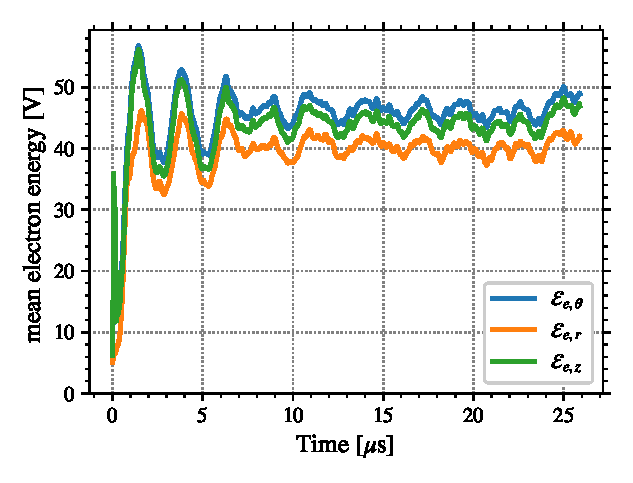
\includegraphics[width=\defaultwidth]{canonical_Te_all_directions_long}
    \caption{Temporal evolution of the electron mean kinetic energy decomposed over the three directions, similar to \cref{fig-canon_Te_strat} but for a longer period. We still see the difference between $\Ee_z$ and $\Ee_{\theta}$ due to the $E\times B$ drift, and the colder radial energy.}
    \label{fig-canon_Te_all}
  \end{figure}
  

  \Cref{fig-profiles} shows the azimuthally-averaged radial profiles of the electron and ion densities.
  The plasma is mostly quasineutral, except close to the walls, in the sheath, where the electron density falls more rapidly compared to that of ions.
  The sheath length can be roughly estimated to be $1\,\milli\meter$.
  The Debye length in our conditions is
  \begin{equation} \label{eq-debye}
    \lambda_D = \sqrt{\frac{\epsilon_0 k_b T_e}{n_e e^2}} \sim 0.4\,\milli\meter,
  \end{equation}
  which corresponds to the expected floating sheath length \citep{chabert2014} (a few $\lde$).
  
  \begin{figure}[hbt]
    \centering
    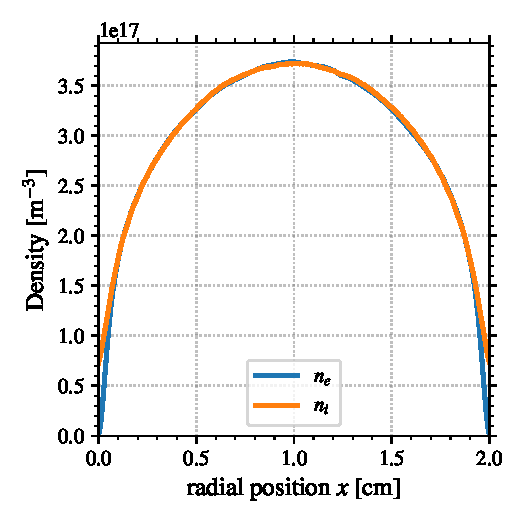
\includegraphics[width=\defaultwidth]{density_profile.pdf}
    \caption{Radial profile of the ion and electron densities at steady-state, averaged azimuthally and in time over the 5 last microseconds.}
    \label{fig-profiles}
  \end{figure}
  
  \subsection{Enhanced electron transport} \label{subsec-canonmue}
  As introduced in \cref{sec-transport}, the electron cross-field axial transport is characterized by the electron mobility
  \begin{equation} \label{eq-mobdef}
    \mob = \frac{u_{e, z}}{E_z}
  \end{equation}
  with $u_{e,z}$ and $E_z$ the electron mean axial velocity and the axial electric field, respectively.
  \nomenclature[Q]{\ensuremath{ \mob}}{ Electron mobility}
  \nomenclature[Q]{\ensuremath{ u}}{ Electron mean velocity}
  In \ac{PIC} simulations, $\mob$ is computed at each time step by
  \begin{equation} \label{eq-mobpic}
    \mobpic = \frac{1}{N E_z} \sum_N v_{e,z}
  \end{equation}

  \begin{figure}[hbt]
    \centering
    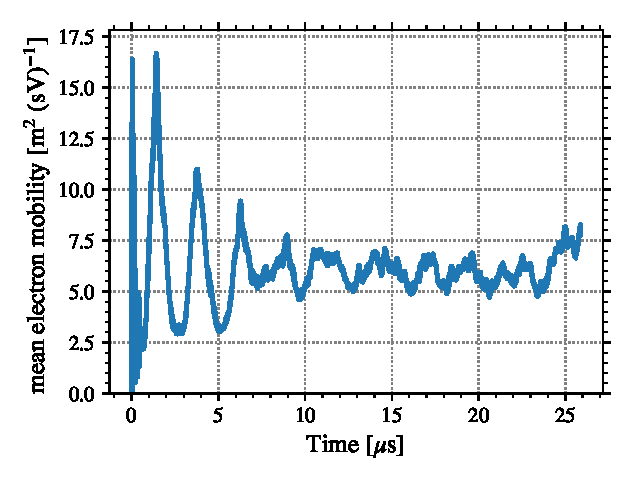
\includegraphics[width=\defaultwidth]{canonical_mu_all}
    \caption{Temporal evolution of the electron axial mobility computed in the \acs{PIC} simulation.}
    \label{fig-canon_mu}
  \end{figure}
  
  \Cref{fig-canon_mu} shows the temporal evolution of the electron mobility $\mobpic$ measured in the simulation with \cref{eq-mobpic}.
  We can see that it presents the same characteristics as the evolution of the electron energy $\Ee$ on \cref{fig-canon_Te_all}.
  We recall that the classical electron mobility from the collisional theory developed in \cref{eq-mobility} is \citep{lafleur2016a}
  \begin{equation} \label{eq-muclass}
    \mobcla = \frac{\nu_m \frac{e}{m_e}}{\oce^2 + \nu_m^2}
  \end{equation}
  with $\nu_m$ the electron-neutral  collision frequency and \oce{} is the electron cyclotron frequency.
  In the conditions of \cref{parameters}, $\mobcla \simeq 0.8$ \square\meter(sV)$^{-1}$.
  
  The measured electron mobility in the \ac{PIC} simulation is one order of magnitude larger than the classical mobility.
  In the present case, as no electron is emitted from the wall, the enhancement can only come from the instabilities present in the plasma.

  % K_ex = 2 10^-13
  % n_g = 1e19
  % wce = q B / m
  The oscillations can be seen in \cref{fig-2dschemat}, which shows the azimuthal electric field observed at $T=4\,\micro\second$.
  It clearly features the oscillation of wavelength of the order of 1~mm, as observed in \citet{heron2013}, and \citet{janhunen2018}.
  \Cref{fig-exampleECDI} shows the temporal evolution of the azimuthal electric field measured at the center of the channel.
  We can see that the instability rises and saturates quickly.
  Then, the oscillation remains quite stable.
  The Fourier Transform of the electric field presents a clear maximum at $14\,\mega\hertz$.
  The theoretical frequency of the \ac{ECDI} instability is \citep{lafleur2017}
  \begin{equation} \label{eq-maxfeq}
    f_{\rm max} = \frac{\omega_{pi}}{\sqrt{3}} \simeq 21 \,\mega\hertz,
  \end{equation}
  which gives a relatively good agreement with the oscillation observed.
  The \ac{ECDI} instability was the subject of \Cref{ch-5}, hence it will not be further discussed here.
  
  
  \begin{figure}[hbt]
    \centering
    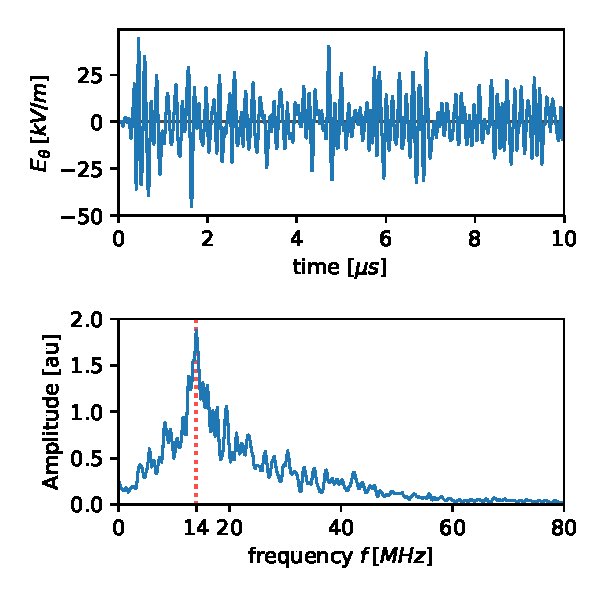
\includegraphics[width=\defaultwidth]{time_and_FFT}
    \caption{Azimuthal instability\string: temporal evolution of the azimuthal electric field at the center of the simulations, and its frequency spectrum computed by \acs{FFT}. The frequency for which the amplitude is maximum is highlighted.}
    \label{fig-exampleECDI}
  \end{figure}
  
  The effective mobility $\mobeff$ is determined by the correlation term $<\dEt \dne>$ and the parameters of the simulations.
  The effective mobility at saturation $\mobeffsat$, using the hypothesis of saturation by ion-wave trapping, only needs the electron temperature $\Te$.
  We can see that the three values $\mobpic, \mobeff$, and $\mobeffsat$ are close from each-others.
  
  \begin{table}[!hbt]
  \ra{1.3}
    \centering
    \caption{Characteristics  measured in the simulation at $t=27\,\micro\second$.}
    \label{tab-canonical_mobility}
    \begin{tabular}{@{} r l @{}} \toprule
    Quantity & Value \\ \midrule
    Correlation $<\dEt \dne>$ & $\sn{6}{20}$ V/m${^4}$ \\
    Effective mobility $\mobeff$ from \cref{eq-eq_mobeffsimple_two} & 4.4 m$^2$(sV)$^{-1}$ \\
    Mobility saturation $\mobeffsat$ from \cref{eq-mobeffsat} & 3.3 m$^2$(sV)$^{-1}$ \\
    Measured mobility $\mobpic$ from \cref{eq-mobpic} & 6 m$^2$(sV)$^{-1}$\\
    \bottomrule
    \end{tabular}
  \end{table}
  

  
  
% !TEX root=/home/tavant/these/manuscript/src/manuscript.tex

\section{Modeling the dielectric layer }
  \label{sec-diel_layer}
  
  The first effect of the wall material studied is adding a layer of dielectric material with its own permittivity, as introduced in \Cref{sec-diel}.
  The simulation parameters are the same as in the canonical case, presented in \cref{sec-canonical}, but the plasma is separated from the ground wall by a dielectric layer of 3~mm.
  Hence, the distance between the grounded electrodes is $2.6\,\centi\meter$.
  The relative permittivity of the dielectric is $\epsr=25$.
  %% SEE runs 250et 257 ?? Ly=1cm, Diel avec et sans SEE
  
  \Cref{fig-diel_radial_Er} shows the radial profile of the radial electric field $E_R$ at $t=10\,\micro\second$ averaged in the azimuthal direction.
  The plasma domain starts at $r=0$ and finishes at $r=2\,\centi\meter$.
  We note the jump in the value of the electric field at the plasma-wall transition.
  This jump is due to the surface charge.
  We can also notice that in the dielectric layer, in $r < 0$ and $r > 2\,\centi\meter$, the radial electric field is close to zero, compared to the value in the sheath.
  
  \begin{figure}[hbt]
    \centering
    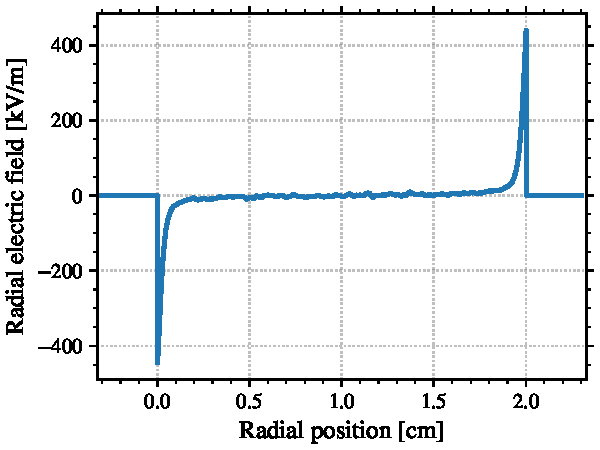
\includegraphics[width=\defaultwidth]{diel_average_radial_electric_field}
    \caption{Radial profile of the radial electric field $E_R$ averaged in the azimuthal direction at $t=10\,\micro\second$. The plasma domain starts at $r=0$ and finishes at $r=2\,\centi\meter$. The dielectric length is $L_{\\rm Diel} = 3\,\milli\meter$.  }
    \label{fig-diel_radial_Er}
  \end{figure}
  
  The next sections investigate the impact of the dielectric layer on the plasma characteristics, and highlight the plasma-wall interaction.
  
  \subsection{Effect of the dielectric layer} \label{subsec-effect_mob}
    
  
  The simulation results are qualitatively the same as in the case without the dielectric layer.
  As an example, \Cref{fig-mod_diel_comp} shows the temporal evolution of the axial electron mobility with and without the dielectric layer.
  We see that the results for the electron temperature and mobility are similar.
  The low amplitude oscillation of the case with the dielectric decreases slightly slower.
  
  \begin{figure}[hbt]
    \centering
    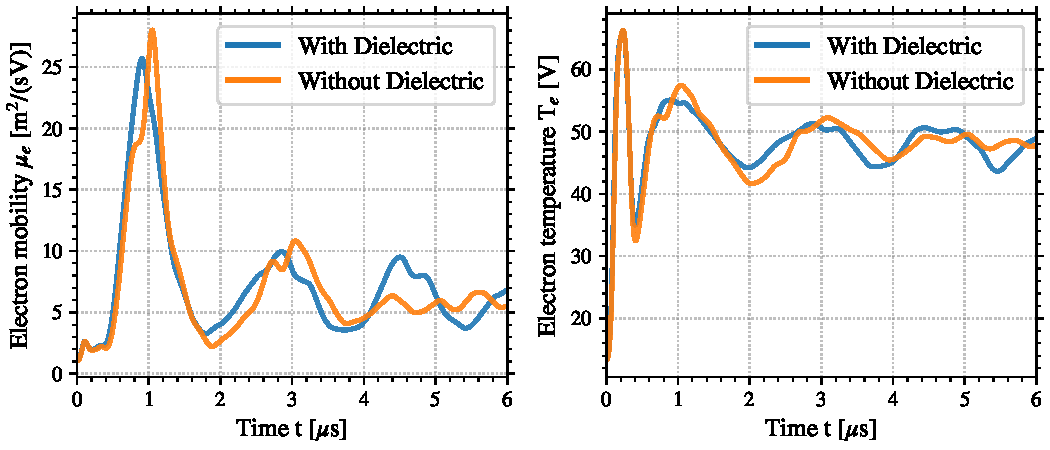
\includegraphics[width=\textwidth]{Dielectric_noSEE_temporal.pdf}
    \caption{Temporal evolution of the axial electron mobility (left), and the electron temperature (right) with and without the dielectric layer modeled.}
    \label{fig-mod_diel_comp}
  \end{figure}

  
  \subsection{Near-wall and in-wall parameters} \label{subsec-nearwall}
    In this section, we focus on the surface charge and the near-wall electric field.
    \Cref{fig-sigma_time} shows the temporal evolution of the surface charge at one point of the wall.
    The position has been chosen to be the center ($L_{\theta} = 0.25$~cm) of the lower wall, but the observations are similar at other positions.
     
    \begin{figure}[hbt]
      \centering
      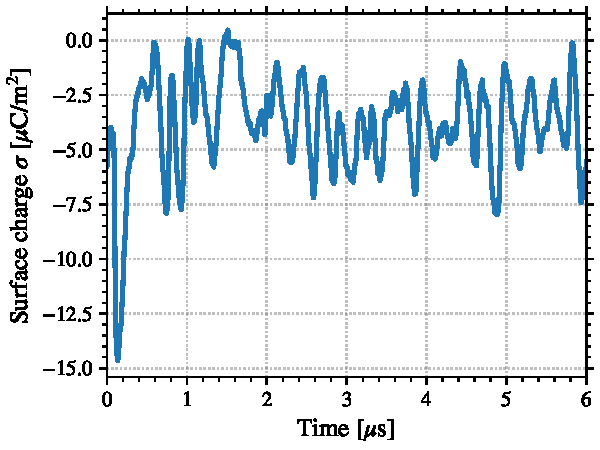
\includegraphics[width=\defaultwidth]{temporal_sigma}
      \caption{Temporal evolution of the surface charge $\sigma$ at one position of the lower dielectric wall}
      \label{fig-sigma_time}
    \end{figure}

    We can see on \cref{fig-sigma_time} that the value of the surface charge start by decreasing significantly (increasing in absolute value), due to the hot electrons that reach quickly the walls.
    Then, $\sigma$ growth and oscillates around a mean value close to $-3.5 \,\micro\coulomb/\square\meter$ and with an amplitude of approximately $1.2 \,\micro\coulomb/\square\meter$.
    
    \cref{fig-indiel} shows the azimuthal evolution of the radial electric field inside the dielectric layer.
    The electric field is given at three different positions ($r=-0.2, -0.9,$ and $-1.8\,\milli\meter$ away from the plasma-wall interface) to highlight its evolution.
    We can see that, even thought there is no charge in the dielectric, the amplitude of the electric field decreases when going further away from the plasma.
    This is due to the \ac{2D} Poisson equation, which smooth-out the inhomogeneity.
     
    \begin{figure}[hbt]
      \centering
      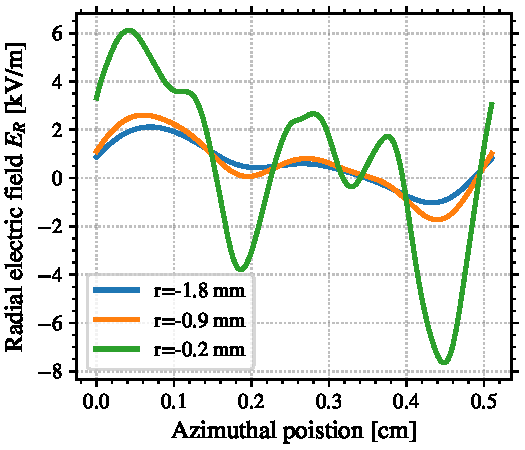
\includegraphics[width=\defaultwidth]{Radial_electric_feld_in_diel.pdf}
      \caption{Azimuthal evolution of the radial electric field inside of the dielectric layer at three different positions; the reference $r=0$ is the plasma-wall interface, the grounded electrode is located at $r=-3\,\milli\meter$.}
      \label{fig-indiel}
    \end{figure}

    
  \subsection{Dielectric model comparison} \label{subsec-modelcomp}
  
  \inlinenote{Anne: {\bf Beaucoup de remarques sur cette partie: pas assez claire, décrire plus les valeures observées, etc. Voir les notes sur le pdf (22 juillet)}}
  
  As introduced in \cref{sec-diel}, a simplified approach to model the effect of the surface charges on the plasma is to use a Neumann boundary condition \citep{taccogna2019}
  \begin{equation} \label{eq-neuman}
    E_r = \frac{\sigma}{\epsilon_0}.
  \end{equation}
  \Cref{eq-neuman} uses two approximations\string:
  \begin{itemize}
    \item one dimensional
    \item No electric field in the dielectric
  \end{itemize}
  We have already seen in \cref{fig-indiel} that the electric field in the dielectric is not zero, but instead it oscillates in respect to the azimuthal instability present in the plasma.  
  \Cref{fig-spacial_comparaison} shows the radial electric field at the wall and compares it to would be obtained by \cref{eq-neuman}.
  We can see that the two values are of the same order of magnitude, close to $-500$~kV/m.
  However, the two values are not equal, as they oscillates around their mean value.
  We can see that the surface charge oscillates more than the actual electric field obtained by solving the Poisson equation.

\begin{figure}[hbt]
  \centering
  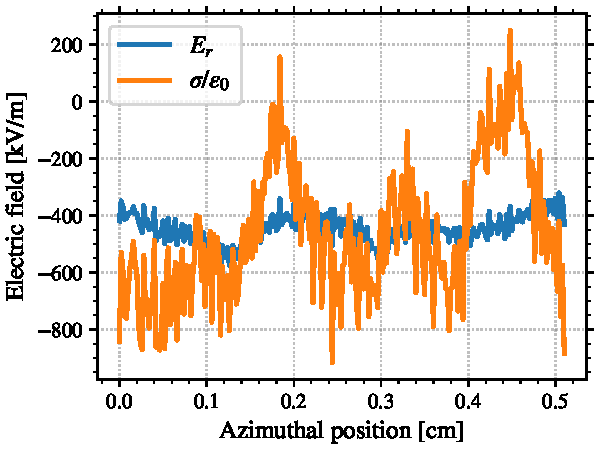
\includegraphics[width=\defaultwidth]{Radila_electric_field.pdf}
  \caption{Azimuthal evolution of the radial electric field at the plasma-wall interface and the electric field that would result from surface charge according to \cref{eq-neuman}.}
  \label{fig-spacial_comparaison}
\end{figure}
\renewcommand\subfigurewidth{0.45\textwidth}

  As a conclusion, we have observed that the dielectric layer does not change the simulation results much, but it can modify the surface processes.
  The model use here for the dielectric layer does not modify the performance of the simulation, while allowing to take into account the \ac{2D} effects.
  In this section, no secondary electron emission has been taken into account.
  In \cref{sec-fulldiel}, we will discuss the influence of using the simplified \cref{eq-neuman} in the case where secondary electron emission is important.

  
% !TEX root=/home/tavant/these/manuscript/src/manuscript.tex

\section{Impact of the radial boundary conditions on the oscillation}
  \label{subsec-BC}

  In \Cref{sec-DR-BC}, we discussed the choice of the radial wavenumber of the instability observed.
  Changing the radial electric boundary condition could affect the instability.
  Therefore, we discuss in this section  the impacts of the dielectric electrostatic boundary condition on the oscillation.
  We have seen in \Cref{sec-diel_layer} that the dielectric boundary did not affect the simulation results macroscopic.
  \Cref{fig-closswallosci} shows the radial evolution in the first few cells of the amplitude of the oscillation of the azimuthal electric field on the left, and the ion density on the right, with grounded (metallic) wall and dielectric wall.
  
  \begin{figure}[!hbt]
    \centering
    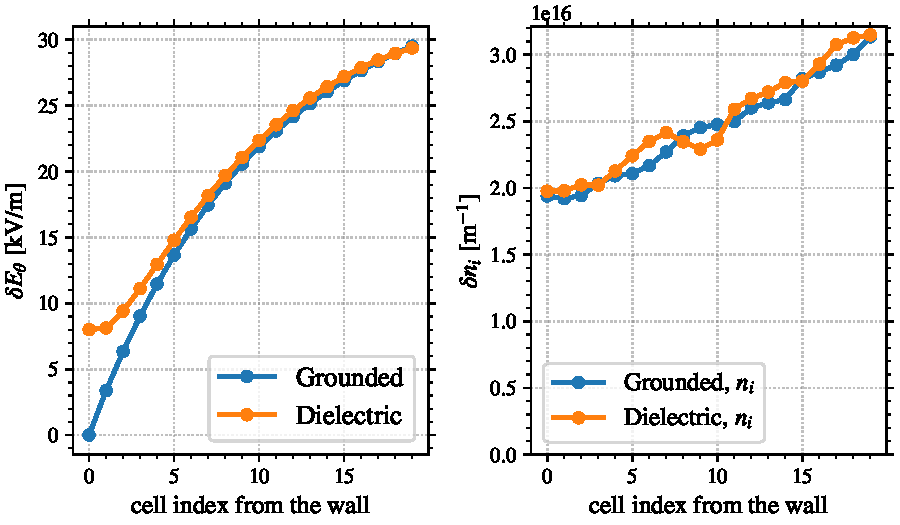
\includegraphics[width=\textwidth]{Ex_closewall.pdf}
    \caption{Radial evolution in the first cells of the amplitude of the oscillation of (left) the azimuthal electric field and (right) the ion density, with grounded (metallic) wall and dielectric wall.}
    \label{fig-closswallosci}
  \end{figure}
  
  We can see in \cref{fig-closswallosci} that the boundary condition does not affects the ion oscillations.
  This is consistent with the observation in \cref{subsec-kr} that the ion fluctuation was not affected by the wall.
  On the other hand, the azimuthal electric field has to go to zero when the wall is grounded.
  In contrast, using the dielectric boundary condition, the azimuthal electric field at the wall limit can be more than zero.
  Indeed, as seen in \cref{fig-indiel}, the amplitude of the azimuthal electric field decreases toward zero inside of the dielectric layer.
  
  Nevertheless, the difference in $E_{\theta}$ between the two boundary conditions quickly disappears inside the plasma domain.
  Indeed, after a dozen cells, corresponding to a few Debye lengths, the amplitudes of $\delta E_{\theta}$ are equal for both cases.
  Hence, the electrostatic boundary condition induces only minor differences in the instability and therefore the plasma discharge.
  
  
% !TEX root=/home/tavant/these/manuscript/src/manuscript.tex

\section{Effect of electron emission}
  \label{sec-see}
  
  In \Cref{sec-canonical}, the walls are not emissive.
  However, the dielectric ceramic used in \ac{HET} can emit electrons \citep{villemant2018,barral2003a}.
  The electron emission model used, introduced in \cref{sec-modelused}, has three parameters $\proba_0, \crover, \probamax$, such that the emission probability depends on the kinetic energy of the incident electron $\ek$ as
  \begin{equation} \label{eq-barral_second}
    \proba = \min \lp \proba_0 + (1 -  \proba_0) \frac{\ek}{\crover}, \probamax    \rp.
  \end{equation}
  
  The value of parameters are summarized in \cref{tab-tabe_parameters_see}.
  The crossover energy $\crover$ is varied from as low as 4~V, corresponding to a very emissive material, to as high as 200~V, a less emissive material.
  
  \begin{table}[hbtp]
  \ra{1.3}
    \centering
    \caption{Parameters of the electron emission probability model}
    \label{tab-tabe_parameters_see}
    \begin{tabular}{@{}ll@{}} \toprule
    Parameter & value  \\ \midrule
    $\proba_0$ & 0.5  \\
    $\probamax$ & 2.9 \\
    $\crover$   &  4  -- 200 V\\
    \bottomrule
    \end{tabular}
  \end{table}
  
  \begin{figure}[hbtp]
    \centering
    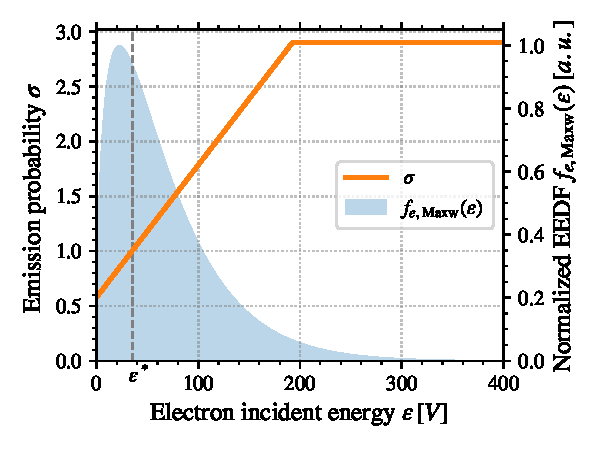
\includegraphics[width=\defaultwidth]{SEE_models}
    \caption{Illustration of the electron emission model of \cref{eq-barral_second} compared to a Maxwellian energy distribution function of temperature of 45~V, with $\crover=35.04$~V.}
    \label{fig-see_illustration}
  \end{figure}
  
  \Cref{fig-see_illustration} shows the electron emission probability for $\crover=35.04$~V compared to a Maxwellian \ac{EEDF} of temperature of 45~V.
  We can see that the saturation of $\proba$ at $\probamax$ happens only for the very high energy tail.
  In the simulation, we can only measure the average electron emission yield, also named emission rate, 
  \begin{equation} \label{eq-seeyield}
    \rate = \frac{\Gamma_{\rm emitted}}{\Gamma_{\rm incident}} = \frac{\iiint v_r \proba(\vect{v}) f(\vect{v}) d^3v}{\iiint v_r  f(\vect{v}) d^3v}.
  \end{equation}
  In general, \cref{eq-seeyield} cannot be calculated analytically.
  However, if we suppose that the \ac{EEDF} is Maxwellian and neglect the saturation at $\probamax$, \cref{eq-seeyield} yields
  \begin{equation} \label{eq-seemaxw}
    \ratemaxw(\Te) = \proba_0 + (1 - \proba_0) \frac{2 \Te}{\crover}.
  \end{equation}
  The saturation at $\probamax$ can be neglected as we have seen that it only affects a small part of the electron population, see \cref{fig-see_illustration}.
  \inlinenote{Add the exact calculation and the relative error ? \\Anne: oui. si trop long, a mettre en annexe.}
  
  \subsection{Impact of the electron emission of the mobility} \label{subsec-param-mob}
    
  The effects of the electron emission at the wall on the electron axial mobility are presented in \Cref{fig-mob-epsstar}.
  The measured mobility $\mobpic$ are shown, as well as the effective mobility $\mobeff$, the saturation estimate $\mobeffsat$ and the classical mobility $\mobcla$, defined in \cref{sec-transport} respectively by \cref{eq-mudef}, \cref{eq-defmobeff}, \cref{eq-mobeffsat} and \cref{eq-mobclas}.
  The values are averaged in time between $t=5 \mus$ and $t=10\mus$, and in space over the azimuthal and radial directions.
  \inlinenote{Anne: For epsilon=0, we have the values presented in section 2.2 without dielectrics.}
  \begin{figure}[hbtp]
    \centering
    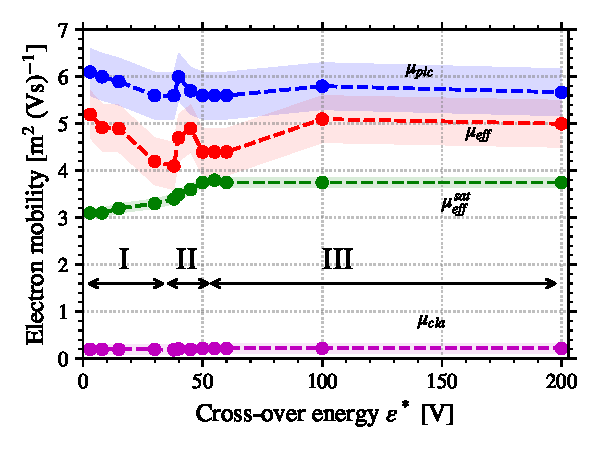
\includegraphics[width=\defaultwidth]{parametric_mobs_eps_complete}
    \caption{Evolution of the electron mobility as a function of the crossover energy $\crover$. In blue $\mobpic$ is the mobility measured in the simulations, while $\mobcla, \mobeff$ and $\mobeffsat$ in purple, red and green respectively are calculated with \cref{eq-mudef,eq-mobclas,eq-defmobeff,eq-mobeffsat}. The three regimes {\bf I, II} and {\bf III}, described in \cref{subsec-regimes} are identified.}
    \label{fig-mob-epsstar}
  \end{figure}
  \inlinenote{Units, in italic !}
  
  As expected, the classical mobility in  \cref{fig-mob-epsstar} is underestimated by more than one order of magnitude compared to $\mobpic$.
  The effective mobility $\mobeff$ and the effective mobility at saturation $\mobeffsat$  are much closer to $\mobpic$, with an underestimation of roughly 10\% and 30\% respectively.
  The mobility measured in the simulation does not evolve much with the electron emission, even for very high emission rate, i.e very low values of $\crover$.
  
  On the other hand, $\mobeffsat$ decreases slightly when $\crover$ decreases from around 40V to lower values.
  However, it still provides a reasonable approximation of the electron enhanced mobility, even with high electron emission rate. 
  
  \subsection{Near wall conductivity}
  
  The results presented in \cref{subsec-param-mob} are spatially averaged.
  However, the mobility coming from the  instability is expected to be higher where the instability is larger, hence at the center of the channel.
  On the other hand, the mobility due to wall emission is located close to the wall \citep{morozov1972}.
  
  \Cref{fig-radial-data} presents the radial profiles of the mobility measured in the \ac{PIC}  simulations without electron emission and for three values of $\crover$.
  On the left, the measured mobility $\mobpic$ is shown and on the right it is the effective mobility $\mobeff$ given by \cref{eq-defmobeff}.
  
  \begin{figure}[hbtp]
    \centering
    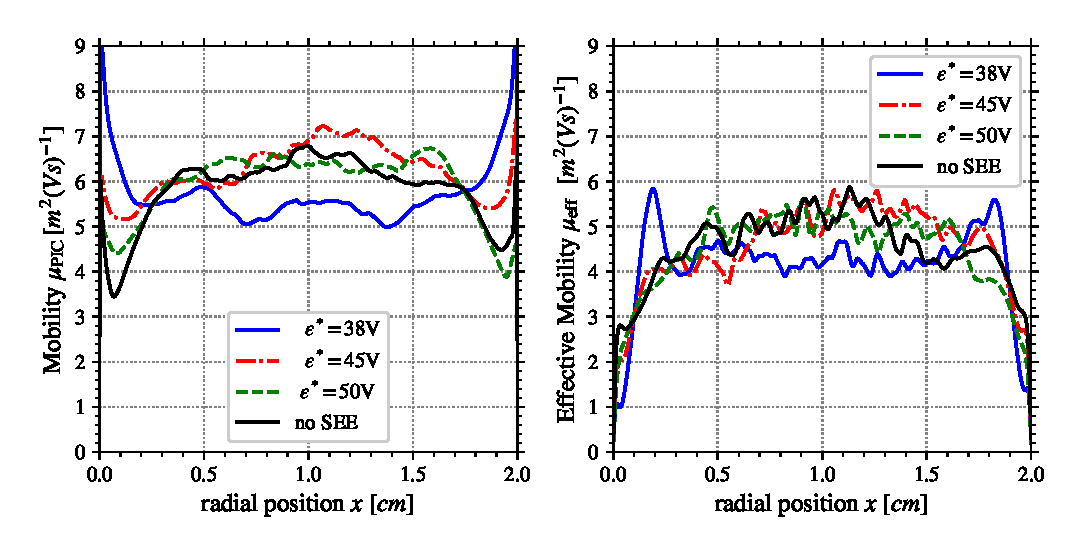
\includegraphics[width=\textwidth]{both_Mobility_SEE}
    \caption{Radial profile the electron mobility (left) measured in the \ac{PIC} simulations, and (right) given by \cref{eq-defmobeff}, for different wall emissivities. }
    \label{fig-radial-data}
  \end{figure}
  
  We can see in \cref{fig-radial-data} that the mobility measured $\mobpic$  in the center decreases by roughly 20\% as the emission rate increases.
  This observation is in agreement with $\mobeffsat$ observed in \cref{fig-radial-data,fig-mob-epsstar}.
  This is due the electron temperature $\Te$ which decreases from around $\Te=45$V at $\crover=200$V to $\Te=30$V at low $\crover$ (the evolution of $\Te$ can be seen in \cref{fig-Tevsproba}).
  
  On the other hand, the near wall mobility increases significantly on $\mobpic$ (almost by a factor of 2) with the increase of the electron emission.
  However, we do not see this evolution on $\mobeffsat$, meaning that it indeed comes from another physical mechanism than the \ac{ECDI}.
  
  
  \subsection{Three different regimes}
  \label{subsec-regimes}

  In \Cref{fig-mob-epsstar}, three regimes have been identified.
  Regime {\bf I} corresponds to low values of $\crover$ (lower than 35V), during which $\mobeffsat$ increases with $\crover$ but $\mobpic$ and $\mobeff$ decreases.
  Regime {\bf III} corresponds to high values of $\crover$ (higher than 50V), during which $\mobeffsat$, and  $\mobpic$ are roughlty constants, but $\mobeff$ increases slightly.
  Regime {\bf II} is a short transition regime, for $35 < \crover < 50$V.
  
  The different regimes are actually obvious when looking at the temporal evolution of the different variables.
  \Cref{fig-threeregimes}  presents the temporal evolution of the space average $\ratepic$ for three different
  values of $\crover$ , corresponding to three different regimes we have identified.
  In regimes {\bf I} and {\bf III}, $\ratepic$ reaches a steady state after a few microseconds.

  \begin{figure}[hbtp]
    \centering
    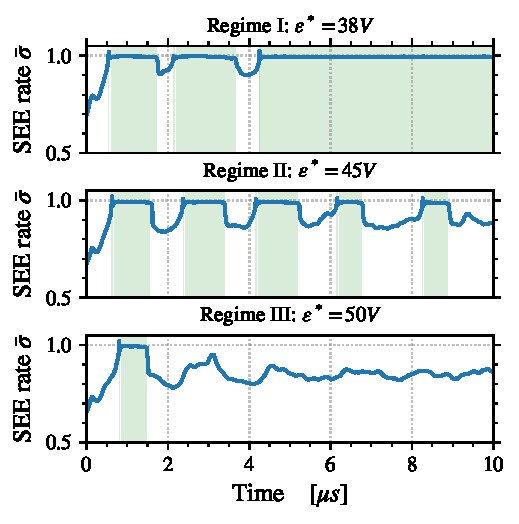
\includegraphics[width=\defaultwidth]{comparaison_3_regimes}
    \caption{Evolution as a function of time of the averaged electron emission rate $\ratepic$ in the three regimes observed (two stables, one with oscillations). The light green zones correspond to the periods when $\ratepic > \ratecr$}
    \label{fig-threeregimes}
  \end{figure}
  

  Regime {\bf I}, with low $\crover$, is characterized by a saturation of $\ratepic$ at a value between $\ratecr$ and 1, which leads to a non-monotonic potential profile.
  Regime {\bf III}, for higher $\crover$, is characterized by a steady state with a SEE rate lower than $\ratecr$.

  The transition between these two stable regimes (monotonic and non-monotonic sheath) passes by regime {\bf II}, an oscillating mode between the two stable regimes.
 As shown in \cref{fig-mob-epsstar}, regime {\bf II} is observed only in a narrow range of $\crover$.
 The oscillations of regime {\bf II} are shown in \cref{fig-threeregimes} up to $10\mus$ but have been observed for more than $40\mus$.
 Note that regimes {\bf I} and {\bf III} in \cref{fig-threeregimes} are obtained for $\crover = 38$~V and $\crover = 50$~V respectively, i.e. near the boundary of the unstable window (see \cref{fig-mob-epsstar}).
 Consequently, we observe a few oscillations before the steady-state is reached, as these cases are close to the bifurcation.
   
   
   The physical origin of the bifurcation can bee seen with the help of \cref{fig-dphivsTe}, which shows the evolution of the potential drop to the wall as a function of the electron temperature.
   It is computed using \cref{eq-seemaxw} for $\rate$ and \cref{eq-sheathhobbs} for the potential drop, which is summarized as 
   \begin{equation} \label{eq-dphi_vs_Te_Maxw}
     \begin{cases}
       \rate = \proba_0 + (1- \proba_0) \frac{2 \Te}{\crover} \\
       \dphi = \Te \ln \lp [1 - \rate] \sqrt{ \frac{m_i}{2 \pi m_e}}  \rp
     \end{cases}
   \end{equation}

   \begin{figure}[hbtp]
     \centering
     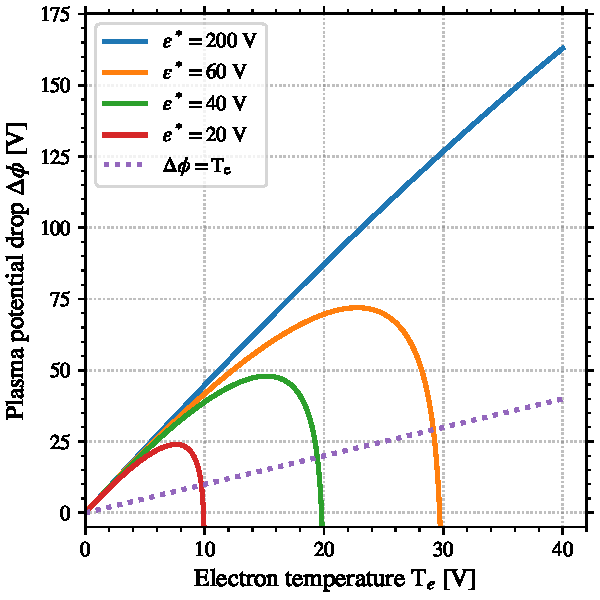
\includegraphics[width=\defaultwidth]{RSO_theo_sheath_bis}
     \caption{Plasma potential drop to the wall as a function of the electron temperature for different values of the cross-over energy $\crover$ using \cref{eq-dphi_vs_Te_Maxw}. The dashed line is $\dphi=\Te$. }
     \label{fig-dphivsTe}
   \end{figure}
   
   \Cref{fig-dphivsTe} shows the evolution of $\dphi$ as a function of $\Te$ obtained with \cref{eq-dphi_vs_Te_Maxw} using four different values of $\crover$. 
   We can see that, starting from low electron temperature, the potential drop increases with the electron temperature, resulting in a better screening of the electrons.
   This corresponds to regime {\bf III}.
   However, the $\dphi$ reaches a maximum, after which it drops sharply to zero and below.
   
   When the potential passes the maximum, the electrons are not screened by the sheath any more.
   Hence, the electrons reach the wall with a higher energy, resulting in a higher electron emission from the wall, hence a smaller potential drop.
   The sheath is unstable, and quickly attains a \ac{SCL} regime \citep{raitses2005}.
   
   In this regime, the sheath is not monotonic, and the model of \cref{eq-sheathhobbs} is no more valid, and the potential drop tends toward $\dphi \simeq \Te$ \citep{hobbs1967,goebel2008} \footnote{see \cref{sec-sheath} for more details}, shown in \cref{fig-dphivsTe}.
   This corresponds to regime {\bf I}.
   
   However, during regime {\bf I}, the electron power losses to the wall are very high, and they can exceed the gains.
   Hence, the electron temperature decreases.
   If $\Te$ decreases too much, the sheath can come back to the previous regime {\bf III}.
   The oscillations between regime {\bf I} and {\bf III} defines regimes {\bf II}.
      
   We have seen in \ref{fig-canon_Te_all} that without electron emission, $\Te$ is of the order of $45$~V.
   Using \cref{fig-dphivsTe}, we can expect to observe the transition between regime {\bf III} and {\bf II} for $\crover \gtrsim 60$~V, as for $\crover = 60$~V, the maximum of $\dphi$ is at $\Te\sim 25$~V, which is significantly lower than 45~V.
   The fact that regime {\bf II} appears at $\crover=50$~V can be explained because
   \begin{enumerate}
     \item a lower $\crover$ increases the electron losses, hence decreases the electron temperature at equilibrium,
     \item the electrons are not Maxwellian.
   \end{enumerate}
   
   The evolution of the temperature with $\crover$ is shown in \cref{fig-Tevsproba}.
   We can see that $\Te \simeq 45\,\volt$ for emission rate up to $\sigma = 0.8$, and decreases down to $\Te=30\,\volt$ for higher emission rates.
   Consequently, even if $\Te$ does indeed decreases when increasing $\crover$, it remains too large compared to the observations of \cref{fig-dphivsTe}.
   The impact of second point will be studied in \cref{ch-3}.
   
   
  
% !TEX root=/home/tavant/these/manuscript/src/manuscript.tex

\section{Validation of the sheath model }
  \label{sec-sheath_validation}
  
  The \ac{PIC} simulations used here do not need any sheath theory in order to model the plasma-wall interaction.
  Conversely, they rely on first principle models.
  Hence, they can be used in order to validate the sheath model introduced in \cref{sec-sheath} coming from the fluid theory.
  
  This sheath model links with \cref{eq-dphi_vs_Te_Maxw} the plasma potential drop $\dphi$ with the electron temperature $\Te$ and the electron emission rate $\rate$.
  \Cref{eq-seemaxw} can be used to estimate the electron emission rate given the mean electron temperature measured in the simulations, corresponding statistically to the plasma bulk temperature.   
  In the \ac{PIC} simulations, $\rate$ can be computed using \cref{eq-seeyield} by counting the number of electrons attaining the wall and emitted during a time-step.
  We note \ratepic this measurement.
  \vspace{1em}
   
  \begin{figure}[hbt]
    \centering
    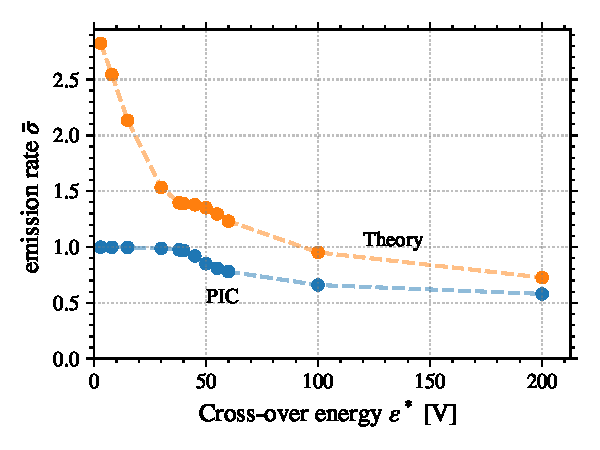
\includegraphics[width=\defaultwidth]{SEE_rates}
    \caption{Values of the electron emission rate $\ratepic$ (blue) measured in the \acs{PIC} simulations, and $ \ratemaxw$ obtained with \cref{eq-seemaxw} using the electron temperature shown in \cref{fig-Tevsproba}. }
    \label{fig-seeparamesMaxw}
  \end{figure}
  
  
  We can see in \Cref{fig-seeparamesMaxw} that the mean electron emission rate lies between 0.6 for large $\crover$ and 1 at low $\crover$.
  The saturation of $\ratepic$ at 1 for high emissivity ( $\crover < 50 \volt$) was not expected from \ratemaxw.
  Indeed, $\probamax$ is equal to 2.9, and the electron temperature in the bulk measured, when used in \cref{eq-seemaxw}, predicts a rate between 1.4 and 2.8.
  This discrepancy at low $\crover$ is due to the \ac{SCL} regime.
  \citet{hobbs1967} predicted that in this regime, a potential well forms such that a fraction of the emitted electrons return to the wall, in order to maintain the effective emission rate to $\ratecr\sim1$.
  However, for $\crover > 50 \volt$, the sheath regime described in \cref{sec-sheath} should be valid.
   
  \begin{figure}[hbt]
    \centering
    \begin{tabular}{@{} cc}
      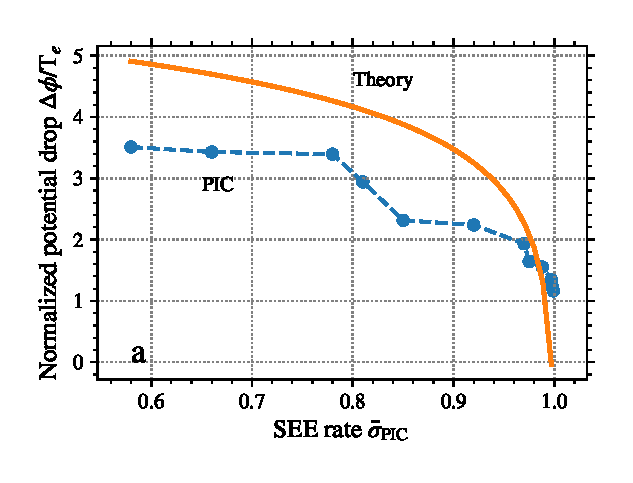
\includegraphics[width=0.45\textwidth]{phi_drop_6}
      &
      \includegraphics[width=0.45\textwidth]{Te_pic_2}
    \end{tabular}
    \caption{({\bf a}) Plasma potential drop to the wall normalized by the electron bulk temperature as a function of the electron rate, and ({\bf b}) the mean electron bulk temperature measured in the \acs{PIC} simulations as a function of the electron emission rate \rate, measured in the simulations, and the effective temperature expected from \cref{eq-Teeff}.  }
    \label{fig-Tevsproba}
  \end{figure}
  
  The electron temperature measured in the bulk of the simulation is presented in \cref{fig-Tevsproba}.{\bf b} for the same cases as in \cref{fig-seeparamesMaxw}.
  An \emph{effective} temperature that would correspond to the measured emission rate $\ratepic$ in \cref{eq-dphi_vs_Te_Maxw},
  \begin{equation} \label{eq-Teeff}
     \ratemaxw(\Te{}_{, eff}) = \ratepic \text{, hence } \Te{}_{, eff} = \frac{\ratepic - \sigo}{1 - \sigo} \frac{\crover}{2},
  \end{equation}
  is also given.
  We can see that when \rate increases, the electron temperature in the bulk $\Te$ monotonically decreases from 45V to around 30V.
  However, these values are not consistent with the measured emission rate \ratepic, even for $\crover > 50\volt$.
  The bulk electron temperature is much higher than the effective $\Te{}_{, eff}$ obtained to correctly predict the emission rate.

  \Cref{fig-Tevsproba}.{\bf a} shows the evolution of the potential drop to the wall measured in the \ac{PIC} simulation compared to the theory  \cref{eq-sheathhobbs} ).
  As expected by \cref{eq-dphi_scl}, $\dphi$ measured in the simulation saturates to $\Te$ for high emission rate ($\ratepic \sim 1$).
  However, we see that at low emission rate, the potential drop is significantly lower than expected.
  The sheath model of \cref{sec-sheath} used two hypotheses\string:
  \begin{itemize}
    \item Maxwellian distribution function to obtain $\ratemaxw$ from \cref{eq-seeyield},
    \item Isothermal electrons in the sheath.
  \end{itemize}
  These two hypotheses will be checked against the PIC simulations in the next chapter.

% !TEX root=/home/tavant/these/manuscript/src/manuscript.tex

\section{Full dielectric model }
  \label{sec-fulldiel}
  
  We have observed the effects of the electron emission and the electrostatic boundary condition separately in \cref{sec-diel_layer,sec-see}, respectively.  
  In \Cref{sec-see}, we observed three regimes depending on the emission rate.
  At high emissivity, the sheath is space-charge limited, resulting in an inverse sheath.
  At low emissivity, we obtain the standard sheath model with electron emission.
  The transition between the regimes passes by a oscillating regime.
  
  In \Cref{sec-diel_layer} we observed that when there is no emission, the dielectric boundary condition for the potential does not change the simulation results.
  In this section, we investigate the interaction between the two characteristics of the dielectric walls, especially with a high emission rate.
  More precisely, regime {\bf II} is the most interesting, as it features a complex behavior.
  Hence, we use $\crover=45\,\volt$ to study the impact of the dielectric layer combined with the electron emission.
  
  The dielectric layer thickness is $L_{\rm Diel} = 3\,\milli\meter$, and the relative permittivity of the dielectric is $\epsilon_R=25$.
  The dimensions of the plasma domain is not modified between the case with and without the dielectric layer.
  Instead, it is the width between the grounded electrodes that is increased.
  
  \subsection{Impact of the dielectric boundary condition on the mobility with electron emission}
    
    \Cref{fig-temporal_mu} shows the temporal evolution of the electron mobility measured in the simulation $\mobpic$ for both cases, with and without the dielectric layer.
    We can see that the two variables are quite similar, with similar mean values and oscillation.
    Interestingly, the beginning of the simulations, up to $t=3\,\micro\second$, are almost identical.
    After this, the values are not in phase.
    
    \begin{figure}[hbt]
      \centering
      \includegraphics[width=\defaultwidth]{dielectron_yesSEE_mobility}
      \caption{Temporal evolution of the axial electron mobility measured in the \acs{PIC} simulation with and without the dielectric layer between the plasma and the grounded electrodes. The crossover energy is $\crover=45\,\volt$, the length of the dielectric layer is $L_{\rm Diel}=3\milli\meter$ and its relative permittivity is $\epsilon_R = 25$.  }
      \label{fig-temporal_mu} 
    \end{figure}
    
    
    \subsection{Plasma-wall interaction}

  
  \begin{figure}[hbt]
    \centering
    \begin{tabular}{@{} c c}
      \subfigure{see_diel_temporal}{a}{20,20} & 
      \subfigure{see_diel_space}{b}{20,20}
    \end{tabular}
    \caption{Comparison of the ({\bf a}) temporal and ({\bf b}) spatial evolution along the dielectric surface of the radial electric field at the wall calculated in PIC simulations compared to the electric field derived from the surface charge. }
    \label{fig-seediel_Er}
  \end{figure}
  \inlinenote{Anne: pas clair le choix des echelles de temps... Refaire ces figures avec les nouveaux resultats}
   
  \Cref{fig-seediel_Er} shows the ({\bf a}) temporal and ({\bf b}) spatial evolution along the dielectric surface of the radial electric field at the wall calculated in PIC simulations compared to the electric field derived from the surface charge, similarly  to \cref{fig-spacial_comparaison}.
  We can see that in contrast to the results of \cref{sec-diel_layer}, the two values are significantly different.
  The electric field measured in the \ac{PIC} simulation is rather uniform and constant, compared to the electric field at the surface calculated only based on the surface charge.
  Moreover, in \cref{fig-seediel_Er}.{\bf a}, we see that at around $t=2.1\,\second$, the electric field sign changes, meaning that the sheath passes from the \ac{SCL} regime {\bf I} to the normal regime {\bf III}, which is typical of regime {\bf II}.
  In contrast, the electric field derived from the surface charge does not shows this change of sheath regime.
  
  
  \begin{figure}[hbt]
    \centering
    \includegraphics[width=\defaultwidth]{dielectron_yesSEE_SEErate}
    \caption{Temporal evolution of the mean electron emission rate $\ratepic$ for the same parameter $\crover=45\,\volt$, with and without the dielectric layer modeled.}
    \label{fig-rso_diel}
  \end{figure}
  
  \cref{fig-rso_diel} compares the temporal evolution of the mean electron emission rate $\ratepic$ for the same parameter $\crover=45\,\volt$, with and without the dielectric wall modeled.
  As previously, the dielectric width is $3\,\milli\meter$, and the electrodes are now $2.6\,\centi\meter$ apart (the geometry of the plasma domain is kept constant).
  We see that the oscillations occur for the two models.
  However, we can observe several differences.
  The first is the lower level of emission rate.
  When the walls are grounded, $\ratepic$ decreases at around $85\%$.
  Conversely, with the dielectric layer included, the emission rate does not decrease much below $95\%$.
  This results in a different overall mean emission rate, that can affect the particle and power balances, hence the mean electron temperature and the performance of the thruster.
  
  
  
  
  
% !TEX root=/home/tavant/these/manuscript/src/manuscript.tex

\section{Conclusion of the parametric study}
  \label{sec-conclusion_ch2}
  
  Using the \ac{PIC} simulation code introduced in \cref{ch-1}, we studied the effects of the dielectric walls on the discharge, and more precisely the effects on the electron axial mobility.
  To begin with, a \emph{base} case with metallic walls was defined and studied.
  The metallic walls correspond to grounded and non-emissive walls.
  For this reference case, we observed that the convection model used allows us to obtain a quasi steady-state.
  We observed an enhanced electron transport transverse to the magnetic field lines, because of the azimuthal instability.
  Both effects of the dielectric -- the electron induced electron emission and the electrostatic boundary condition -- were investigated.
  First, we  only modeled the dielectric boundary condition. Then, we studied only the electron emission. Afterwards, the two phenomena have been studied together.
  
  \subsubsection*{Electrostatic boundary condition}
  
  The electrostatic boundary condition is modeled by including in the domain of simulation the thickness of the wall ($L_{\rm Diel} = 3 \milli\meter$).
  Surface charges accumulate at the interface between the plasma and the wall.
  We observed that the modified boundary condition did not modify significantly the discharge and the axial cross-field electron mobility.
  Moreover, we saw that the boundary condition used results in a radial electric field $E_r$ of the same order of magnitude than the Neumann boundary condition of \cref{eq-neuman} but the spatio-temporal evolution is not identical.
  
  Indeed, when the secondary electron emission is modeled, the surface charges oscillates significantly compared to the radial electric field during the \ac{SCL} regime.
  As the dielectric model used here do not increase significantly the computational time, we recommend to use it instead of the Neumann boundary condition, that do not reproduce the same plasma-wall interaction.
  
  
  \subsubsection*{Electron induced electron emission}
  
  The electron  emission from the wall due to the impact of primary electron reaching the wall is modeled using the model described in \cref{sec-seemodel}.
  The value of the crossover energy $\crover$ is varied from a large value (low emissivity) to small values (high emissivity).
  We observed in the simulations that when the electron emission rate increases, the mean electron temperature decreases.
  This decreases the amplitude of the \ac{ECDI} at saturation, hence decreases the electron mobility in the plasma (see \cref{fig-radial-data}).
  However, electron emission induces \ac{NWC}, which almost doubles the electron mobility close to the wall when $\crover$ varies from $200\volt$ to $30\volt$.
  Consequently, the overall electron cross-field mobility is almost constant in our simulation.
  
  We observed in our \ac{PIC} simulations three different regimes depending on the values of $\crover$.
  For high values of $\crover$, the plasma stabilises with an emission rate $\ratepic < \ratecr$.
  When $\crover$ is small, we observe a stable configuration with $\ratepic \sim \ratecr$.
  Under these conditions, the sheath is space-charge limited.
  The transition between the two regimes is not stable, but instead passes by a bi-stable regime.
  In this third regime, the sheath jumps between the two stable regimes.
  

  \subsubsection*{Inconsistent sheath model }
  
  The simulation results have been compared to the sheath model of \citet{hobbs1967}.
  We observed a significant discrepancy between the \ac{PIC} simulations and the sheath model that comes from a fluid approach.
  In particular, the potential drop and the electron emission rate are both overestimated.
  These overestimations can lead to erroneous conclusion and prediction when using fluid models.
  Hence, a better understanding of the plasma-wall transition via the sheath is needed.
  
  The sheath model currently used is based mainly on two hypothesis
  \begin{itemize}
    \item Maxwellian electron distribution function
    \item Isothermal electrons in the sheath
  \end{itemize}
  
  Both hypotheses will be questioned in the next chapter.
  


% \acresetall
% !TEX root=/home/tavant/these/manuscript/src/manuscript.tex




\chapter{Anisothermal sheath}
\label{ch-3}

In order to explain the discrepancy observed in \cref{ch-2} between the simulation and the sheath model, we investigate the simulation data.
We see that the hypothesis of the sheath model do not stand.
Using a simplified \ac{1D} \ac{PIC} simulation, we derive a polytropic closure for the electron.
With this new closure equation, we derived a modified sheath model, that fit well the kinetic simulations. 


{\bf III. Polytrotic sheath model} 23 pages
\begin{zzz}
  This chapter takes the 2nd paper about the modified sheath model

  3.1 EVDF in the 2D PIC simulations of HET.    3 pages

  3.2 1D simplified simulations, Parametric study and polytropic fits. 7 pages

  3.3 Monte-Carlo simulations.  3 pages

  3.4 fluid equations with polytropic closure. 10 pages
\end{zzz}


\minitoc




% !TEX root=/home/tavant/these/manuscript/src/manuscript.tex



\section{Insights for the PIC simulations}
\label{sec-insights}

As announced in \vref{sec-sheath_validation}, the sheath model of \vref{sec-sheath} uses two hypothesis\string:
\begin{itemize}
  \item Maxwellian electrons,
  \item Isothermal evolution of the electrons.
\end{itemize}

When collisions can be neglected, as it is usually assumed in the sheath, these two hypothesis are linked.
Indeed, the \ac{1D} Maxwellian distribution function expressed as the total energy is
\begin{equation} \label{eq-maxw_total}
  f(\ek, \phi) \propto \exp \lp \frac{\ek - \phi}{\Te}  \rp = \propto \exp \lp \frac{\ek}{\Te} \frac{-\phi}{\Te},
\end{equation}
where $\ek$ and $\Te$ are the electron kinetic energy and temperature expressed in Volt.
We can see in \cref{eq-maxw_total} that the spatial variation (due to the plasma potential $\phi$) only affect the amplitude of the distribution function, not its shape in the energy space.
Hence, the electron temperature is uniform, i.e. they are isotherm.
In addition, we find that $n_e \propto \exp (- \phi / \Te)$, which is the definition of Boltzmann electrons.

Hence, let see if this two aspects are respected in the \ac{2D} \ac{PIC}-\ac{MCC} simulation results

\subsection{Electron distribution function}

\begin{figure}[hbtp]
  \centering
  \includegraphics[width=\defaultwidth]{EEDF_2-eps-converted-to}
  \caption{Electron energy distribution function of the electrons ({\bf a}) in the bulk, in the three directions, and ({\bf b}) in the bulk and in the sheath}
  \label{fig-EEDF}
\end{figure}

Using the kinetic information of the PIC simulations, we present in \Cref{fig-EEDF} the mean electron energy probability functions (EEPF) in the case $\crover = 200\,\volt$.
\Cref{fig-EEDF}.{\bf a} shows the projections of the EEPF in the centre of the simulations along the three directions.
These projections are compared to the Maxwellian probability function of the same
kinetic temperature.
\Cref{fig-EEDF}.{\bf b} shows the total EEPF for both the bulk and the sheath populations.
 The sheath length is defined as the location where the ions reach the Bohm speed, which is about 0.4mm.
 
 We see in \cref{fig-EEDF}.{\bf a} that the electron distribution function is not Maxwellian.
 In particular the high energy tails are depleted.
 However, we can see that the electrons are rather isotropic, compared to \ac{1D} simulation \citep{sydorenko2006}.
 In order to evaluate the effect of the nonMaxwellian EEPF, we numerically integrate the EEPF from the PIC data using \vref{eq-ratedifinition_evdf}.
The results (not shown) do not differ significantly from the Maxwellian values of \vref{eq-seemaxw}.
Hence, we can conclude that even if the Maxwellian hypothesis is not respected in the
PIC simulations, it is not enough to explain the differences observed in \vref{fig-seeparamesMaxw}.


\Cref{fig-EEDF}.{\bf b} presents the EEPF for the bulk population as well as for the sheath population.
 We can see that the sheath population is colder than the population at the centre, which could explain the difference of \vref{fig-seeparamesMaxw}. 
 This effect is assessed in the next section.



 


% \acresetall
% !TEX root=/home/tavant/these/manuscript/src/manuscript.tex




\chapter{Polytropic sheath model in the presence of electron emission}
\label{ch-4}
\headerchaptername{Anisothermal sheath model with emission}

\inlinenote{Anne: a reflechir: si seulement chapitre de 10 pages...a rajouter en derniere partie du 3?
Mais je pense que c'est a rediscuter en fonction de ce que tu vas mettre dans la fin du chapitre 4.
Un chapitre plus court que les autres ce n'est pas genant non plus ;-)}

\begin{Chabstract}
  
%e modify the polytropic sheath model with secondary electron emission
We add to the non-isothermal sheath model developed in \cref{ch-3} the secondary electron emission.
Using the \ac{PIC} simulations with secondary emission, we observe that the electrons are well described by a polytropic index, which is almost constant when varying the cross-over energy $\crover$.
Hence, we derive the sheath characteristics using the same fluid approach.
We note that this model allows multiple solutions for a given electron temperature, which could explain the oscillations observed in regime {\bf II}.
The predictions of the polytropic sheath model are successfully compared to the \ac{PIC} simulation results presented in \cref{ch-2}.
%The modified sheath model is included in a \ac{1D} fluid model.
\end{Chabstract}

% {\bf IV. Polytrotic sheath model with SEE} 20 pages
% \begin{zzz}
%   This chapter goes beyond the actual modified sheath model in order to add SEEs.
%   This require some time to develop before writting !
% 
%   5.1 Kinetic effects of the SEE on the EVDFs  4 pages
% 
%   5.2 SEE effects on the Fluid model  5 pages
% 
%   5.3 Validation against the Parametric 2D PIC simulation results. 2 pages
% 
%   5.4 1D fluid model with modified wall model. 4 pages
% 
%   5.4Bis Global model (Vivien's) with modified wall model. 4 pages
% \end{zzz}

\minitoc
% 
% What is complicated here is the definition of the electron temperature, that include both primary and secondary electrons.
% Should we
% \begin{itemize}
%   \item Use a 2 fluid( so 1 electron) with a fluid model that includes the SEE ?
%   \item Use a 3 fluid model, that would  include folly absorbed primary electrons (simply polytropic) and emitted electrons, with strictly positive velocity.
% \end{itemize}
% 
% In the First case, the electron temperature is simple to define.
% But the closure equation may need to be changed.
% 
% the second case is more simpler, mathematicaly.
% 
% References:
% Il y a déjà eu beaucoup de travaux, mais aucun model fluides !
% 
% \citet{meezan2002} : Bolzmann solver, 2-Te EVDF, SEE compared with Maxwellian
% 
% \citet{smirnov2004} : MCC code, 2-Te EVDF. Mais fake EVDI effect via collisions
% 
% \citet{sydorenko2006a} : Beam in EVDF because of 1D PIC-MCC 
% 
% \citet{raitses2006} : "strong anisotropy : facteur 4",  compare Mesures avec fluids codes: says disagriment. Talks about 
% 
% \citet{ahedo2002} : sheath-presheath model with SEE with bolzmann electron, Sagdeev potential, SCL regime avec saturations 
% 
% \citet{ahedo2003} : 1D axial model avec wall interactions (SEE et SCL), plum with section increase (A(z)) 
% 
% \citet{ahedo2005} : Fluid model with SEE, with partial trapping and partial beams
% 
% \citet{raitses2005} : SCL regime and Te saturation (where he says that the SCL may not be responsible ??)
% 
% \citet{barral2003a} : 1D model, anisotrop electrons ({\bf must read to know how}), shows saturation at SCL with large anisotropy

% {\bf \Large A lire}
% 
% \citet{sydorenko2007} :  non maxwellian EVDF
% 
% \citet{raitses2005a} : electron-wall interaction
% 
% \citet{jolivet2000} : SEE effect on EVDF 

% !TEX root=/home/tavant/these/manuscript/src/manuscript.tex


\section{Polytropic index in the \ac{HET} \ac{PIC} simulations}
\label{sec-PIC_poly}

\begin{figure}[hbtp]
  \centering
  \includegraphics[width=\defaultwidth]{EVDF_Bulk.pdf}
  \caption{Electron velocity distribution function at the center of the simulation, for different values of $\crover$.}
  \label{fig-evdf_epsstar}
\end{figure}

\begin{figure}[hbtp]
  \centering
  \includegraphics[width=\textwidth]{ne_Te_profiles.pdf}
  \caption{Radial profiles of (left) the electron density and (right) the electron temperature, for different values of $\crover$.}
  \label{fig-radial_profiles_see}
\end{figure}


\begin{figure}[hbtp]
  \centering
  \includegraphics[width=\defaultwidth]{SEE_polytropic_presheath_and_sheath.pdf}
  \caption{electron pressure as a function of the electron density normalized by the center variable, in log scale. Markers are every 10 cells (around 1$\lde$)}
  \label{fig-log_pe-ne}
\end{figure}

\renewcommand\subfigurewidth{3in}

\begin{figure}[hbtp]
  \centering
  \begin{tabular}{c c}
    \subfigure{SEE_polytropic_presheath}{a}{20,20} & 
    \subfigure{SEE_polyfit}{a}{20,20} 
  \end{tabular}
  \caption{Polytropic fit for different values of $\crover$. The sheath (10 cells) are removed from the plots.}
  \label{fig-polyfit_see}
\end{figure}

\FloatBarrier
{\bf Conclusion: $\gamma = 1.35$ in presheath and $\partial{\gamma} / \partial \crover = 0 $}

\paragraph{Hypothesis H1: } Polytropic model until the wall and $\gamma = 1.35$ (might be explained by \cref{{fig-evdf_epsstar}}, and by the fact that we care only on the forward temperature, so not distorted by the secondary electrons).

\paragraph{Hypothesis H2: } From {\bf H1}, and with the 2-$\Te$ hypothesis, we have $\rate = \rate_{\rm Maxw}(\Tew)$, were $\Tew$ can be computed from $Teb$, $\gamma$ and $\dphi$.

\paragraph{Hypothesis H3: } Current equality at the wall : $\Gamma_i + \rate \Gamma_e = \Gamma_e$. This is not a surprising hypothesis.

\section{Sheath model with polytropic electron and SEE}

With {\bf H1, H2} and {\bf H3} we have, as developed in \cref{sec-fluidPIC} with \cref{eq-gi,eq-ge,eq-tew}:
\begin{equation}\label{eq-sheathsee}
  (1 - \rate_{\rm Maxw}(\Tew) )\left[ 1 +\frac{\gamma -1}{\gamma} \frac{ \dphi_0}{ \Te_0}  \right]^{\frac{1}{\gamma - 1}} \sqrt{1 - \frac{\gamma -1}{\gamma}\frac{\dphi_0}{\Te_0}} = \sqrt{\frac{4 \gamma \pi m_e}{m_i}}
\end{equation}
In contrast with \cref{eq-sheath}, now the sheath potential $\Delta \phi$ depends on $\rate$ with depends on $\Te$.
Hence, $\dphi$ is not fully normalized.

\begin{figure}[hbtp]
  \centering
  \includegraphics[width=\defaultwidth]{Sheath_drop_with_SEE.pdf}
  \caption{Potential drop $\dphi$ normilized by the bulk electron temperature $\Te_0$ as a function of the polytropic index $\gamma$ for a xenon plasma ($m_i = 131\,\dalton$). The emission rate $\rate$ is fixed for clarity.}
  \label{fig-dphi_see}
\end{figure}

\begin{figure}[hbtp]
  \centering
  \includegraphics[width=\defaultwidth]{RSO_criteria_polytropic.pdf}
  \caption{ Plasma potential drop to the wall as a function of the electron temperature for different values of the cross-over energy $\crover$ using \cref{eq-sheathsee,eq-seemaxw}. The dashed line is $\dphi=\Te$. Similar to  \cref{fig-dphivsTe} but with polytropic electron of index $\gamma=1.35$}
  \label{fig-rso_crit_see}
\end{figure}

\FloatBarrier

\section{Comparison with PIC simulations} \label{subsec-picandmodel}

\begin{figure}[hbtp]
  \centering
  \includegraphics[width=\textwidth]{dphi_polytropic_noSEE}
  \caption{PIC simulation results (with SEE) compared to the polytropic limit without SEE.}
  \label{fig-polytropic_pic_noSEE}
\end{figure}

\begin{figure}[hbtp]
  \centering
  \includegraphics[width=\textwidth]{Summary_polytropic_SEE.pdf}
  \caption{Comparison of the PIC simulation results with the polytropic model with SEE.}
  \label{fig-polytropic_see_summary}
\end{figure}



% !TEX root=/home/tavant/these/manuscript/src/manuscript.tex

% \FloatBarrier
\section{Sheath model with polytropic electrons and electron emission}
\label{sec-fluid_poly_see}

\let\oldrightmark=\rightmark
\renewcommand\rightmark{\expandafter\MakeUppercase{Sheath with polytropic electron and SEE}}


\subsection{Definition of the sheath equation} \label{subsec-def_sheat_see}

We have seen in \cref{sec-PIC_poly} that even in the presence of electron emission from the wall, the electrons can be described using a polytropic state law.
The value of the polytropic index obtained from the mean electron density and temperature is for $\crover \geq 40 \,\volt$ is $\gamma = 1.36$.
% Using the electron distribution function, the evolution of the forward electron seems to follow a polytropic low of index $\gamma=1.28$.
Hence, we modify the polytropic sheath model of \cref{sec-fluid} to take into account the electron emission from the wall.
This modifies the current equality at the wall to
\begin{equation} \label{eq-see-J_eq}
  \Gamma_i = (1 - \rate) \Gamma_e.
\end{equation}

\paragraph{Sheath model with constant emission rate\\}

Using \cref{eq-gi,eq-ge,eq-tew} for $\Gamma_i$ and $\Gamma_e$, we obtain the equality
\begin{equation}\label{eq-sheathsee}
  (1 - \rate )\left[ 1 +\frac{\gamma -1}{\gamma} \frac{ \dphi_0}{ \Te_0}  \right]^{\frac{1}{\gamma - 1}} \sqrt{1 - \frac{\gamma -1}{\gamma}\frac{\dphi_0}{\Te_0}} = \sqrt{\frac{4 \gamma \pi m_e}{m_i}}
\end{equation}

Similarly to the case without electron emission in \cref{sec-fluid}, \cref{eq-sheathsee} cannot be solved analytically, but it can be solved numerically.
The solution for $\rate=0.8$ is compared to the case without electron emission ($\rate=0$) for a \ac{Xe} plasma in \cref{fig-dphi_see}.
As expected, the potential difference decreases with increasing $\rate$.
We see that the gap between the two cases decreases when $\gamma$ increases from 1 to 2.

\begin{figure}[!hbt]
  \centering
  \includegraphics[width=\defaultwidth]{Sheath_drop_with_SEE.pdf}
  \caption{Potential drop $\dphi$ normalized by the bulk electron temperature $\Te_0$ as a function of the polytropic index $\gamma$ for a xenon plasma ($m_i = 131\,\atomicmass$). The emission rate $\rate$ is fixed either at $\rate=0$ or $\rate=0.8$.}
  \label{fig-dphi_see}
\end{figure}

\paragraph{Sheath model with varying emission rate\\}

In fact the electron emission rate is a function of the electron temperature at the wall.
Using the same hypothesis as in \cref{eq-ge} (mostly a Maxwellian \ac{EVDF} at the wall), we define the emission rate from \cref{eq-seemaxw} by
\begin{equation} \label{eq-seemaxw_poly}
  \rate = 
  \begin{cases}
    \ratemaxw(\Tew) =  \sigo + ( 1 - \sigo) \frac{ 2 \Tew  }{\crover} \\
    \ratecr \text{ \quad, if } \ratemaxw(\Tew) > \ratecr
  \end{cases}
\end{equation}
with $\ratecr = 0.983$ corresponding to the \ac{SCL} regime, and the electron temperature at the wall
\begin{equation} \label{eq-Tewall}
  \Tew = \Teb - \frac{\gamma - 1}{\gamma } \dphi.
\end{equation}


Noting $\chi = \frac{\gamma -1}{\gamma} \frac{ \dphi_0}{ \Teb} $, we finely obtain the sheath equation to be solved
\begin{equation} \label{eq-costseepoly}
  f(\chi) = \left[ 1 + \chi  \right]^{\frac{1}{\gamma - 1}} \sqrt{1 - \chi} - \frac{  \sqrt{4 \gamma m_e / m_i}}{1 - \rate (\Teb, \chi )} = 0.
\end{equation}

\Cref{eq-costseepoly} depends now explicitly on $\Teb$ though $\rate$.
Hence, the solution of $f(\chi)=0$ is no longer independent of $\Teb$, which adds a free parameter when solving the sheath equation.
\Cref{fig-costfunction} shows the evolution of $f(\chi)$ of \cref{eq-costseepoly} for $\gamma = 1.36$, $\Teb=40\,\volt$ and $\crover=50\,\volt$.

\begin{figure}[!hbt]
  \centering
  \includegraphics[width=\defaultwidth]{cost_function_solo}
  \caption{Value of $f(\chi)$ of \cref{eq-costseepoly} for $\gamma = 1.36$, $\Teb=40\,\volt$ and $\crover=50\,\volt$. The five red triangular markers represents five points of interest\string: the three markers S1, S2, and S3 are solutions of $f(\chi) = 0$; and the markers A and B are two local extrema. }
  \label{fig-costfunction}
\end{figure}

We see that $f(\chi)$ of \cref{eq-costseepoly} is rather complex.
Five points of interest are marked and labeled in \cref{fig-costfunction} to ease the reading\string: 
\begin{enumerate}
  \item S1, S2, and S3 represents the points at which $f(\chi)=0$, i.e. the solutions of  \cref{eq-costseepoly}
  \item A and B are two local extrema.
\end{enumerate}

The courbe $f(\chi)$ is composed of two continuous branches that join at the point A in \cref{fig-costfunction}.
The two branches corresponds to the two cases of \cref{eq-seemaxw_poly}. Hence, the point A corresponds to the value of $\dphi/\Teb$ for which  \[ \sigo + ( 1 - \sigo) \frac{ 2 \Tew  }{\crover} = \ratecr = 0.983. \]

The branch at the left of A corresponds to the \ac{SCL} regime, and has one solution S3 to $f(\chi)=0$ at $\dphi / \Teb \simeq 1$.
This solutions is the same as in the isothermal case \citep{hobbs1967}.
The branch at the right of A passes by a local maximum B and presents two roots S1 and S3.

The existence of the three solutions depends on the values of $\crover$, $\Teb$ and $\gamma$.
\Cref{fig-costfunction_multiple} shows the impact of the evolution of $\Teb$ and $\crover$, with $\gamma$ constant.
We can see that when $\Teb$ decreases, or $\crover$ increases, the points A and B move upward.
Consequently, for low values of $\Teb$ (respectively large values of $\crover$) the point A can be above the line $f(\chi) = 0$, hence  \cref{eq-costseepoly} presents only the root S1.
In contrast for high values of $\Teb$ (respectively low values of $\crover$) the point B is below $f(\chi) = 0$, so that only S3 is solution of  \cref{eq-costseepoly}.
For intermediate values of $\Teb$ and $\crover$, A and B are located on both sides of $f(\chi) = 0$, so that the three roots S1, S2, and S3 exist.
\renewcommand\subfigurewidth{0.47\textwidth}

\begin{figure}[!hbt]
  \centering
  \begin{tabular}{@{} c c}
    \subfigure{cost_function_bis.pdf}{a}{25,25} &
    \subfigure{cost_function_2bis.pdf}{b}{25,25} \\
  \end{tabular}
  \caption{Value of $f(\chi)$ of \cref{eq-costseepoly} for $\gamma = 1.36$ and different values of $\Teb$ and $\crover$. ({\bf a}) shows the impact of the evolution of $\Teb$ with $\crover=50\,\volt$, and ({\bf b}) shows the impact of the evolution of $\crover$ with $\Teb=35\,\volt$. }
  \label{fig-costfunction_multiple}
\end{figure}

\Cref{fig-schematic-solutions} illustrates the three coexisting sheath solutions.
The red solid line  with the largest potential drop to the wall represents the solution S1, which is the standard sheath.
This solutions leads to the largest electron temperature drop to the wall, hence the smallest \ac{SEE} rate.
The dashed blue line, with a potential well close to the wall, corresponds to the root S3 in the \acs{SCL} regime, for which $\rate=\ratecr$ and with $\dphi \simeq \Teb$.
Lastly, the dash-dotted green line represents S2 the intermediate solution.
 
\begin{figure}[hbtp]
  \centering
  \includegraphics[width=\defaultwidth]{sheath_solutions.png}
  \caption{Schematic representation of the plasma potential profile in the sheath to the wall for the three coexisting solutions. The red solid line is the standard solution, with the lowest \acs{SEE} rate; the dashed blue line corresponds to the \acs{SCL} regime, with $\rate=\ratecr$; the dash-dotted green line is the intermediate solution, with an intermediate \acs{SEE} rate.  }
  \label{fig-schematic-solutions}
\end{figure}



\Cref{fig-iso_poly} shows the evolution of the sheath potential drop and the \ac{SEE} rate as a function of $\Teb$ for the case $\crover=50\,\volt$.
Both the isothermal sheath and the polytropic model using $\gamma=1.36$ are showed. 
The result of the isothermal sheath model was previously shown in \cref{fig-dphivsTe}  in \cref{ch-2}.
For the solution of the polytropic sheath model, the branches corresponding to the three solutions S1, S2, and S3 are labeled.
The light green area highlights the temperature range with the three coexisting solutions.
The lower bounds of the area is noted $\Te^2$ and the upper bound is noted $\Te^1$
\renewcommand\subfigurewidth{0.65\textwidth}

\begin{figure}[!hbt]
  \centering
  \begin{tabular}{@{} c}
    \subfigure{Iso_vs_poly_dphibis}{a}{25,18} \\
    \subfigure{Iso_vs_poly_rate}{b}{20,18} 
  \end{tabular}
  \caption{Evolution as a function of the electron temperature $\Te$ for $\crover=50\,\volt$ of ({\bf a}) the plasma potential drop to the wall $\dphi$, and ({\bf b}) the SEE rate $\ratemaxw$ using the polytropic sheath model ($\gamma = 1.36$) and the isothermal sheath model. The labels S1, S2 and SCL regime correspond to the three solutions illustrated in \cref{fig-schematic-solutions}. The light green area highlights the temperature range with three solutions.}
  \label{fig-iso_poly}
\end{figure}

\renewcommand\subfigurewidth{0.47\textwidth}

We see in \cref{fig-iso_poly}.{\bf a} that $\dphi$ is significantly impacted by the polytropic law.
In particular the maximum potential drop which is more than twice as high as the isothermal maximum.
In addition, we see in \cref{fig-iso_poly}.{\bf b} that the polytropic sheath model predicts a \ac{SEE} rate smaller than the isothermal model.
This is due to the fact that the polytropic state law reduces the electron temperature at the wall, hence decreases the electron emission rate for a given $\Teb$.
Consequently, the electron bulk temperature can access higher temperature, compared to the one observed in \cref{fig-dphivsTe}.


\subsection{Theoretical values of the critical electron temperatures} \label{subsec-theo_Tecr}

  As shown in \cref{fig-costfunction}, for a given $\Teb$ $f(\chi)$ defined by  \cref{eq-costseepoly} presents a local minimum and a local maximum, labeled A and B respectively in \cref{fig-costfunction}.
  Therefore, there exist two values of $\Teb$ for which either the minimum or the maximum of the $f(\chi)$ crosses exactly the horizontal axis.
  These values, noted $\Te^1$ and $\Te^2$ corresponds respectively to the upper and lower bounds of the electron temperature range over which the three solutions coexist.
  These threshold temperatures can be seen for $\gamma=1.36$ in \cref{fig-iso_poly}, where $\Te^1\simeq 55\,\volt$ and $\Te^2\simeq 35\,\volt$ 

  \paragraph{Maximum electron temperature value for regime {\bf III}, $\Te^1$\\}

    The first critical electron temperature  $\Te^1$  corresponds to the maximum temperature of the root S1, which is the usual monotonic sheath (corresponding to regime {\bf III}).
    It is defined as the temperature for which the the local maximum B crosses the line $f(\chi)=0$.
    As it is a double solution, it corresponds to the solution of \cref{eq-costseepoly} that is also a solution of its derivative with respect to $\chi$\string:
    \[ \deriv{f(\chi)}{\chi} = 0. \]
    Once again, the equation is not trivial, and cannot be solved analytically, thus we solve it numerically.

    \begin{figure}[hbt]
      \centering
      \begin{tabular}{@{} cc}
        \subfigure{Maximum_Te1_epsilon.pdf}{a}{20,20} &
        \subfigure{Maximum_Te1_gamma.pdf}{b}{20,15} \\
      \end{tabular}
      \caption{Variation of $\Te^1$  ({\bf a})  as a function of $\crover$ for two values of $\gamma$, and ({\bf b})  as a function of $\gamma$ for two values of $\crover$.}
      \label{fig-Te1_epsi}
    \end{figure}

    \Cref{fig-Te1_epsi} shows the variation of $\Te^1$ as a function of   $\crover$  and $\gamma$.
    We see that the maximum temperature $\Te^1$ increases linearly with $\crover$.
    This was expected, as in \cref{eq-costseepoly}, the only time that $\Teb$ is explicitly present is in the term $\frac{\Teb}{\crover}$.
    On the other hand, the variation with $\gamma$ follows a power law, monotonically increasing from $30\,\volt$ for $\gamma=1.2$ to $50\,\volt$ for $\gamma=1.4$ in the case $\crover=45\,volt$.

  \paragraph{Minimum electron temperature value for regime {\bf I}, $\Te^2$\\}

    The minimum electron temperature value for regime {\bf I}, $\Te^2$, corresponds to the case where the electron temperature at the wall induces exactly an emission rate $\ratemaxw (\Tew) = \ratecr$.
    Noting $C_1 = \frac{\ratecr - \sigo}{1-\sigo} = 0.964$, we obtain
    \begin{equation} \label{eq-Te2}
      (1-\ratecr) \lp 2 - \frac{C_1 \crover}{2 \Te^2} \rp^{\frac{1}{(\gamma-1)}} \sqrt{\frac{C_1 \crover}{2 \Te^2}} = \sqrt{\frac{4 \gamma \pi m_e}{m_i}}
    \end{equation}

    \Cref{eq-Te2} is solved numerically.
    The solutions for different values of $\crover$ and $\gamma$ are shown in \cref{fig-Te2_epsi}.
    As for $\Te^1$, $\Te^2$ increases linearly with $\crover$.
    It also increases slowly with $\gamma$, from $26\,\volt$ for $\gamma=1.2$ to $30\,\volt$ for $\gamma=1.4$ in the case $\crover=45\,volt$.
    We note that $\Te^2$ increasing more slowly with $\gamma$ compared to $\Te^1$, hence the range of temperature with the three coexisting solutions widen  when $\gamma$ increases.

    \begin{figure}[hbt]
      \centering
      \begin{tabular}{@{} cc}
        \subfigure{Maximum_Te2_epsilon.pdf}{a}{20,25} &
        \subfigure{Maximum_Te2_gamma.pdf}{b}{20,20} \\
      \end{tabular}
      \caption{Variation of $\Te^2$  ({\bf a}) as a function of $\crover$ for two values of $\gamma$, and ({\bf b}) as a function of $\gamma$ for two values of $\crover$.}
      \label{fig-Te2_epsi}
    \end{figure}

% 
% \subsection{Resolution of the sheath equation} \label{subsec-sol_sheat_see}
% \inlinenote{should I keep this section ?}
% 
% \Cref{fig-rso_crit_see} shows the evolution of the sheath potential drop with the electron temperature for different values of $\crover$.
% It is similar to \cref{fig-dphivsTe} but with the use of a polytropic state law for the electrons.
% Two main aspects differ compared to the isothermal model\string: the multiple solutions and the maximal electron temperature of the first solution.
% 
% \begin{figure}[hbt]
%   \centering
%   \includegraphics[width=\textwidth]{Potential_drop_poly_see.pdf}
%   \caption{ Plasma potential drop to the wall as a function of the electron temperature for different values of the cross-over energy $\crover$ using \cref{eq-costseepoly}. It is the same results as  \cref{fig-dphivsTe} but with polytropic electron of index $\gamma=1.35$.}
%   \label{fig-rso_crit_see}
% \end{figure}
% 
% We observe in \cref{fig-rso_crit_see} that the electron temperature in the center $\Teb$ can be much higher before the inversion of the plasma sheath potential, compared to \cref{fig-dphivsTe}.


% In addition, for some values of electron temperature, there are three solutions.
% This could explain the oscillations observed in regime {\bf II}.
% Indeed, when the electron temperature increases, the sheath follows the first solutions.
% When the critical electron temperature is reached, the sheath jumps to the third solution.
% It corresponds to the \ac{SCL} regime with an inverted sheath.
% There, the electron temperature in the bulk decreases because of the increased electron power losses at the wall.
% The electron temperature decreases until the second critical temperature, which corresponds to the moment when the third solution disappear, so that the sheath jumps back to the first solution.
% We do not expect the third solution in-between to be observed in the simulations.

% 
% 
% \vspace{1em}
% To summarize, the polytropic law is combined with electron emission to model the sheath.
% The model obtained is richer than the usual isothermal model, as it allows multiple values of potential drop to the wall for the same electron bulk temperature.
% This model only uses the electron bulk temperature and self-consistently computes both the potential drop and the electron emission rate.
% It is compared in the next section to the \ac{PIC} simulation results.


\let\rightmark=\oldrightmark

% !TEX root=/home/tavant/these/manuscript/src/manuscript.tex

% \FloatBarrier

\section{Comparison of the sheath model with PIC simulations} \label{subsec-picandmodel}

  % \begin{figure}[hbtp]
  %   \centering
  %   \includegraphics[width=\textwidth]{dphi_polytropic_noSEE}
  %   \caption{PIC simulation results (with SEE) compared to the polytropic limit without SEE.}
  %   \label{fig-polytropic_pic_noSEE}
  % \end{figure}
  % 
  % \begin{figure}[hbtp]
  %   \centering
  %   \includegraphics[width=\textwidth]{Summary_polytropic_SEE.pdf}
  %   \caption{Comparison of the PIC simulation results with the polytropic model with SEE.}
  %   \label{fig-polytropic_see_summary}
  % \end{figure}

  We compare in this section the characteristics of the plasma wall interaction observed in the \ac{PIC} simulations with the fluid model developed in \cref{sec-fluid_poly_see}.
  We first compare the mean values using in the parametric study over the crossover energy $\crover$, then we investigate the oscillations of regime {\bf II}.

  \subsection{Parametric study of the modified sheath model} \label{subsec-param_sheath_see}

    The variables of interest to characterize the plasma-wall interaction are the averaged electron emission rate $\rate$ and the plasma potential drop to the wall.
    The only input of the modified sheath model is the electron mean temperature in the bulk $\Teb$, as well as the polytropic index $\gamma$.
    As seen in \cref{sec-PIC_poly}, the polytropic index of the electron population is measured in the \ac{PIC} simulations to be $\gamma=1.35$.
    However, the electrons going toward the wall present a different index, measured from the bulk \ac{EVDF} to $\gamma=1.28$.
    These two values will be compared.

    Using the mean electron temperature measured in the \ac{PIC} simulations, we first compute the plasma potential drop $\dphi$ by solving \cref{eq-costseepoly} with $\gamma=1.35$.
    As shown in \cref{fig-rso_crit_see}, up to three solutions are possible.
    The emission rate $\rate$ is then computed using \cref{eq-seemaxw_Tew}, using the two values for $\gamma$.
    As discussed previously, the rate is limited to $\ratecr=0.982$ to take into account the \ac{SCL} regime.

    The results are shown in \Cref{fig-Poly_model_vs_pic}.
    The plasma potential drop computed is increased by $\Teb/2$ corresponding to the pre-sheath drop to better match the plasma potential measured in the simulations.
    \improvement{The Bhom criterion is slightly modified with the polytropic model, so it should not exactly be $\Teb/2$. however, it matches to well here that I do not really want to change !}

    \begin{figure}[hbtp]
      \centering
      \includegraphics[width=\textwidth]{Poly_model_vs_pic}
      \caption{Comparison of the PIC simulations and the sheath model for the plasma potential drop from the center to the wall and the electron emission yield. }
      \label{fig-Poly_model_vs_pic}
    \end{figure}

    Concerning $\dphi$, we see that the sheath model combining the polytropic state law and the electron emission is in good agreement with the \ac{PIC} simulations.
    We see that the region where the three solutions coexist corresponds well with the regime {\bf II}.

    Concerning the emission rate $\rate$, we observe that the value $\gamma=1.35$ under estimates $\rate$ compared to the values of the \ac{PIC} simulations.
    On the other hand, $\gamma=1.28$ is in very good agreement.
    Interestingly, the saturation of the mean electron emission rate in the \ac{PIC} simulation is greater than the critical value $\ratecr$.
    
    %\inlinenote{ As $\rate$ is better with $\gamma=1.28$, we should use both values in \cref{eq-costseepoly}. However, this increases the complexity the equations and the model, and add 1 more free parameters (they would be 2 values for $\gamma$ now). I can say that only in the discussion maybe ? }
    
  \subsection{Sheath oscillations of regime {\bf II}} \label{subsec-pic_scheath_RSO}
  
    The regime {\bf II} is characterized by the presence of oscillations between two meta-stable regimes {\bf III} and {\bf I}, one with a low emissivity and the other with a high emissivity.
    \Cref{fig-long_time} shows the temporal evolution of the electron temperature and the plasma potential relative to the wall for $\crover=45\,\volt$.
    The electron temperature is computed over the whole electron population in the \ac{PIC} simulations.
    Both the radial temperature $\Te_{,R}$ and the total temperature $\Te$ are shown (see \cref{eq-3Te} for their definition).
    The plasma potential $\dphi$ shown is measured at the center of the radial direction of the simulation, averaged over the azimuthal direction.
    
    
    \begin{figure}[hbtp]
      \centering
      \begin{tabular}{c c}
        \subfigure{long_time_dphi}{a}{20,20} &
        \subfigure{long_time_Te}{b}{20,20} \\
      \end{tabular}
      \caption{Temporal evolution of ({\bf a}) the plasma potential $\dphi$ and ({\bf b}) the electron temperatures\string: $\Te_{,R}$ is the radial temperature, and $\Te$ is the total temperature.}
      \label{fig-long_time}
    \end{figure}

    
    We clearly see in \cref{fig-long_time} the quasi-periodic oscillations between the two states.
    We observe that the electron temperature is slightly anisotropic, with the radial temperature smaller than the axial temperature.
    This anisotropy observed was not taken into account in the sheath model.
    More precisely, the $\Te_{,R}$ is linked to the thermal flux of electron toward the wall, while the total temperature $\Te$ is used in the computation of the electron emission rate $\ratemaxw$.
    However, the degree of anisotropy is not very high, as it is of the order of 10\% when the sheath is not inverted.
    When the sheath is inverted, the anisotropy is of the order of 25\%, as the electron with a large radial energy are quickly absorbed.
    However in the \ac{SCL} regime, we suppose that the electron emission rate saturates at $\rate=\ratecr$, hence the impact of the total energy is less important with respect of the radial energy.
    Hence, we will compare the prediction using only the radial temperature $\Te_{,R}$ or the total, averaged, temperature $\Te$, but not the two of them together.
    
    \Cref{fig-dphi_te_PIc} shows the potential drop as a function of the radial electron temperature $\Te_R$ and the total electron temperature $\Te = (\Te_R + \Te_{\theta} + \Te_z)/3$ measured in the \ac{PIC} simulation (same case as \cref{fig-long_time}).
    Is also shown the theoretical solutions obtained with the model of \cref{sec-fluid_poly_see} using a constant polytropic index $\gamma=1.35$ and $\crover=45\,\volt$.
    
    \begin{figure}[hbtp]
      \centering
      \includegraphics[width=\textwidth]{parametric_PIC_dphi_Te_bis}
      \caption{Plasma potential as a function of (left) the radial electron temperature and (right) the total electron temperature. The blue markers represent the \ac{PIC} results presented in \cref{fig-long_time}, and the orange dashed lines correspond to the theoretical values with $\gamma=1.35$.}
      \label{fig-dphi_te_PIc}
    \end{figure}
    
    We see in \cref{fig-dphi_te_PIc} that the sheath characteristics observed in the \ac{PIC}  simulations match relatively well the theoretically values.
    In particular, we see the cohabitation of the two solutions of $\dphi$ observed for the same electron temperature, which corresponds to the domain of electron temperature for which the sheath model also predicts multiple solutions.
    
    During the state corresponding to regime {\bf III} (high value of  $\dphi$), the \ac{PIC} values are too noisy to clearly determine if the sheath follows the first or the second branch of the solutions.
    On the other hand, we see relatively well the correspondance between the \ac{PIC} results and the theory for the regime {\bf I} (low value of $\dphi$).
    
    As discussed previously, the value of the polytropic index computed by propagating the \ac{EVDF}, is $\gamma=1.28$.
    \Cref{fig-dphi_te_PIc2} shows the same results as \cref{fig-dphi_te_PIc}, but  the theoretical values of $\dphi$ using $\gamma=1.28$ are overlaid.
    We see that using the value $\gamma=1.28$ does not change significantly the value of the solution, except for the maximum value of the electron temperature $\Te^1$ for the first branch of the solution, hence the domain of temperature where the three solutions coexist.
    In the case of $\gamma=1.28$, the \ac{PIC} simulation result agreement with the theory is worse than for $\gamma=1.35$.
    
    \begin{figure}[hbtp]
      \centering
      \includegraphics[width=\textwidth]{parametric_PIC_dphi_Te_two_gamma_bis}
      \caption{Similarly to \cref{fig-dphi_te_PIc}, Plasma potential as a function of (left) the radial electron temperature and (right) the total electron temperature. The blue markers represent the \ac{PIC} results presented in \cref{fig-long_time}, the orange dashed lines correspond to the theoretical values with $\gamma=1.35$, and the green dotted-dashed line is computed with $\gamma=1.28$.}
      \label{fig-dphi_te_PIc2}
    \end{figure}
    
    \paragraph{Stationary of the sheath \\}

    One has to note that the modified sheath model is stationary, while the oscillations observed are relatively fast.
    Indeed, the ion dynamic can be estimated to be
    \begin{equation} \label{eq-ti}
      \tau_i = \frac{2 \pi}{\opi} = 0.1 \,\micro\second.
    \end{equation}
    
    Another estimation of the ion time scale is the time needed by an ion to reach the sheath edge from the center of the discharge.
    Supposing a constant electric field $E_{\rm ps} = \frac{\Te}{L_R}$ in the pre-sheath, we have
    \begin{equation} \label{eq-tof}
      t_{\rm flight} = L_R \sqrt{\frac{m_i}{e \Te}} = 3.7 \,\micro\second.
    \end{equation}
    with $L_R=2\,\centi\meter$ and $\Te=40\,\volt$.
    The period of the sheath oscillations observed in \cref{fig-long_time} is approximately $T = 2\,\micro\second$, which is between $\tau_i$ and $t_{\rm flight}$.
    Hence, we can expect the ion dynamic to affect the plasma sheath characteristics during the sheath oscillations of the regime {\bf II}.
    
    \paragraph{Role of the ion mass \\}
    
    The sheath oscillations of regime {\bf II} have been observed in \citet{croes2017} with three different ion masses: xenon, krypton and argon.
    The results are shown in \cref{fig-RSO_altern}.
    We see that the period of the oscillations vary with the ion mass.
    More precisely, the period of oscillation decreases with the decrease of the ion mass.
    This observation confirm that the ions have a role in the dynamics of the oscillation.
    
    \begin{figure}[hbtp]
      \centering
      \includegraphics[width=\defaultwidth]{SEE_RSOs.png}
      \caption{Temporal evolution of the SEE rate $\rate$ measured in the PIC simulations for different gases (xenon, krypton, and argon), taken from \citet{croes2017}.}
      \label{fig-RSO_altern}
    \end{figure}
    
    
% !TEX root=/home/tavant/these/manuscript/src/manuscript.tex

% \FloatBarrier

    
    \section{Electron temperature saturation in experiments}
    
    
    In \citet{raitses2006}, the authors compare the maximum of the axial profile of the electron temperature $\hat{\Te}$ measured in a \ac{HET} with two different wall materials, one with a very low emissivity (carbon velvet material), the other the conventional \ac{BN} ceramic.
    \Cref{fig-raiteses2006} reproduces the results obtained in \citet{raitses2006}.

    \begin{figure}[hbtp]
      \centering
      \includegraphics[width=\defaultwidth]{Raiteses_remaked.pdf}
      \caption{ The dependence of the maximum electron temperature on the discharge  voltage for a conventional thruster with high-SEE \ac{BN} channel walls and the segmented thruster with low-SEE floating segmented electrodes made of carbon velvet material. Reproducibility of measurements is shown by error bars. Adapted from \citet[Fig. 3]{raitses2006} }
      \label{fig-raiteses2006}
    \end{figure}

    They observed that with the \ac{BN} ceramic, the values of $\hat{\Te}$ present a maximum value that cannot be exceeded, while the results with the low emissivity material do not present such maximum.
    The maximum value of $\hat{\Te}$ measured for \ac{BN} ceramic is $\hat{\Te}^1 = 55 \pm 6\,\volt$, the error corresponds to reproducibility of the measurements (manually extracted from \citep[Fig. 3]{raitses2006}, reproduced in \cref{fig-raiteses2006}).
    
    The saturation of the temperature is expected to be due to the \ac{SCL} regime, which increase the electron power losses.
    For a \ac{BN} wall, we have $\crover\simeq 35\,\volt$ \citep{smirnov2004}.
    The value of $\Te^1$ observed experimentally,  $\hat{\Te}^1$, is higher than the value observed in the \ac{PIC} simulations and obtained with the sheath model, which close to $\Te^1 = 45\,\volt$.
    however, the agreement is significantly better than with the isothermal sheath model prediction 
    \begin{equation} \label{eq-Temaxisothermal}
      \Te^1_{\rm , isothermal} \simeq \frac{\crover}{2} \simeq 17.5 \,\volt.
    \end{equation}
    
    One possible explanation of the difference is the anisotropy of the electrons.
    Indeed, the probe measurements measure the average electron temperature, in contrast with the sheath theory which suppose that the electrons are isotropic.
    
% !TEX root=/home/tavant/these/manuscript/src/manuscript.tex

% \FloatBarrier

\section{Utilisation of the modified sheath model} \label{subsec-applcation}

We have developed in the previous section a model for the plasma-wall interaction using a fluid approach, that better reproduce the interaction observed in kinetic simulations.
In this section, we try to use it in a low-dimensional fluid simulation.

\inlinenote{I tried to adapte the global model of Vivien, but it is not working well... I'm not sure what is missing / not well model, so I gave up this part for now.} 

\inlinenote{This modification of the 1D axial Fluid model (\~ Barral, Trevor, Roberto) has to be done. If I don't have time I guess it is not a big deal, but it could be greate to have !}

% \acresetall
% !TEX root=/home/tavant/these/manuscript/src/manuscript.tex




\chapter{Evolution of the azimuthal instability and generalized dispersion relation}
\label{ch-5}

\begin{Chabstract}
  
As briefly mentioned in \cref{ch-1}, the $E \times B$ configuration of the \ac{HET} give rise to azimuthal instabilities.
This aspect has been neglected in \cref{ch-2,ch-3}, except by its consequences on the axial electron transport.
While these instabilities have been the subject of numerous studied, they remain unclear.

Using the results of the \ac{PIC} simulations, we propose new insights for the understanding on the instability, hence the electron cross-field transport.
In particular, we develop a relation dispersion solver that uses the velocity distribution function measured in the simulations.
Then, we compare the simulation instability characteristics with the dispersion relations.
A special care is taken with the boundary condition and the instability non-linear saturation. 
\end{Chabstract}

% 
% 
% {\bf V. analyse of the instability } 30 pages
% \begin{zzz}
%   \begin{itemize}
% \item Instability dispersion relation
% \item Kinetic solver for Ion and ECDI using VDFs
% \item Impact of the difference w/r Maxwellian
% \item Wall Boundary condition, 3D dispertion relation vs 1D and 2D relations
% \item Linear stage as ECDI and Saturation toward IAW
% \end{itemize}
% \end{zzz}

\minitoc


The presence of azimuthal instabilities in the Hall effect thrusters has first been showed with numerical simulations by \citet{adam2004}.
Then, they have been the subject of numerous studies, especially numerical \citep{ducrocq2006,lafleur2016,lafleur2016a,croes2017,croes2018,janhunen2018,taccogna2019}, but also experimental \citep{honore2011,cavalier2013,cavalier2013a}.
However, their nature remain unclear \citep{boeuf2018}.
The investigation of the instabilities observed in the \ac{2D} \ac{PIC} simulations in the subject of this chapter.

In \cref{sec-PIC-ECDI}, we present the oscillations observed in the \ac{PIC} simulations.
After that, we derive the dispersion relation with no hypothesis used concerning the particle distribution functions in \cref{sec-DR-kinetic}, and we present in \cref{sec-DR-solver} a numerical algorithm that solves the dispersion relation using the distribution function measured in the \ac{PIC} simulations.
The oscillations observed in the simulation are compared in \cref{sec-DR-results} to the results of the dispersion relation.
To finish with; the impact of the radial boundary condition is investigated in \cref{sec-DR-BC}.

% !TEX root=/home/tavant/these/manuscript/src/manuscript.tex

\section{Instability in the \acs{2D} radial-azimuthal \acs{PIC} simulations}
  \label{sec-PIC-ECDI}
  
  \subsection{Introduction and state of the art} \label{subsec-indroECDI}
        
    The presence of azimuthal instabilities in the Hall effect thrusters has first been shown with numerical simulations by \citet{adam2004}.
    Then, they have been the subject of numerous studies, especially numerical \citep{ducrocq2006,lafleur2016,lafleur2016a,croes2017,croes2018,janhunen2018,taccogna2019}, but also experimental \citep{honore2011,cavalier2013,cavalier2013a}.
    However, their nature remain unclear \citep{boeuf2018}.
    Viven Croes studied the azimuthal instability in a bi-dimensional (\acs{2D}) radial-azimuthal simulation domain of radial length $L_R=2\,\centi\meter$ and azimuthal length $L_{\theta}=0.5\,\centi\meter$, with the model of particle convection proposed by Lafleur \citep{croes2017,croes2018}.
    He showed that the saturation of the oscillations was due to ion-wave trapping.
    Using a parametric study over the plasma density and the ion mass, he observed that the main oscillation is consistent with the characteristics of the \ac{IAW}.
    
    During the three years of my Ph.D., other groups presented new simulation results in similar radial-azimuthal geometries.
    \citet{hara2019a} presented kinetic simulation results on a two-dimensional domain, of size similar to the case studied here.
    However, that work was focused on the electron mobility values, and few information on the instability are given.
    In \citet{janhunen2018}, the authors presented a collisionless highly resolved \acs{2D} \ac{PIC} simulation.
    No convection and no compensation model for radial losses are used, hence the electron energy quickly rises and the density decreases.
    On the other hand, the domain is bigger, with a radial length of $L_r = 53.8\,\milli\meter$ for an azimuthal length of $L_{\theta} = 13.45 \,\milli\meter$.
    Three cells by Debye length are used, while there are in average 800 particles per cell.
    In these conditions, the instability rises, but a large radial structure, named Modified Two Stream Instability (MTSI), of radial wavelength twice as big as $L_r$  is observed.
    The simulation parameters of \citet{taccogna2019} are similar to the results presented here, with  $L_r = 15\,\milli\meter$ and $L_{\theta} = 12.5 \,\milli\meter$.
    The results are qualitatively similar to the others, however the authors also observed radial structures, but this time with a wavelength of a third of $L_r$.
        
    \vspace{1ex}
    We can see that the results obtained with similar configurations differ significantly, meaning that some points needs to be clarified.
    % Therefore, we present in this chapter the results obtained with \LPPic.  
    In \cref{sec-PIC-ECDI}, we present the oscillations observed in the \ac{PIC} simulations carried out with \LPPic.
    After that, we derive the dispersion relation with no hypothesis concerning the particle distribution functions in \cref{sec-DR-kinetic}, and we present in \cref{sec-DR-solver} a numerical algorithm that solves the dispersion relation using the distribution function measured in the \ac{PIC} simulations.
    The oscillations observed in the simulation are compared in \cref{sec-DR-results} to the results of the dispersion relation.
    To finish with, the impact of the radial boundary condition is investigated in \cref{sec-DR-BC}.


  \subsection{Overview of the 2D simulation} \label{subsec-lppic_ECDI}
  
    
    We present in this section the simulation conducted to study the azimuthal instability.
    The parameters of the simulation are given in \cref{tab-evdfpicparams}.
    The imposed axial electric field $E_z$ and the radial magnetic field $B_r$ are uniform in space and constant in time.
    The radial direction is closed with the dielectric boundary condition of dielectric width $L_{diel}=3\,\milli\meter$.
    No \ac{SEE} is modeled, and the convection is modeled with the new noiseless model (see \cref{sec-noiselessresults}).
    The simulation is initialized with a uniform electron and ion density $n_e = n_i = \sn{3}{17}\per\meter\cubed$, with an electron temperature $\Te=10\,\volt$ and an ion temperature $\Ti=0.025\,\volt$.
    The mean particle density is conserved by imposing an ionization  which compensate the particle losses at the wall a each time step.
    
    \begin{table}[!hbt]
    \ra{1.3}
      \centering
      \caption{Parameters of the \acs{2D} \acs{PIC} simulations}
      \label{tab-evdfpicparams}
      \begin{tabular}{@{}r l l l @{}} \toprule
        {\bf Physical Parameter} &  &   &  \\
      Parameter                    & Symbol                          & Value                    & Unit \\ \midrule
      Dimensions                   & $L_r\times L_{\theta}\times L_z$ & $1\times 0.26\times 0.5$ & cm \\
      Radial magnetic field        & $B_r$                            & 0.02                     & T \\
      Axial electric field         & $E_z$                            & \sn{2}{4}                & $s\volt\per\meter$ \\
      Dielectric layer of width    & $L_{diel}$                       & 3                        & \milli\meter \\
      Mean plasma density          & $n_{0}$                          & $3 \times 10^{17}$       & {m}$^{-3}$ \\
      Initial electron temperature & $\Te_{,0} $                      & $10.0$                   & V \\
      Initial ion temperature      & $\Ti_{,0} $                      & $0.025$                  & V \\
      Duration of the simulation   & $T_{\rm simu}$                   & $7$                      & $\micro\second$ \\
      \midrule
      {\bf Numerical Parameter}    &                                  &                          & \\
      Time step                    & $\Delta t $                      & $4 \times 10^{-12}$      & s \\
      Cell size                    & $\Delta x = \Delta y$            & $2 \times 10^{-5}$       & m \\
      Number of particles per cell & $N/NG $                          & $80$                     & part/cell \\
      \bottomrule
      \end{tabular}
    \end{table}
    
    \Cref{fig-profiles_ne_one} shows the radial profile of the electron and ion densities, as well as the plasma potential, at the end of the simulation, averaged azimuthally and in time between $t=4$ and $7\,\micro\second$.
    The results are averaged azimuthally and in time over the 3 last microseconds.
    We can observe on the radial profile of both the densities and the plasma potential the sheaths close to the walls (regions of high electric field due to a charge unbalance) and the quasineutral plasma bulk in the center.
    These profiles are typical of low temperature low pressure bounded plasmas.
    
    \begin{figure}[hbt]
      \centering
      \begin{tabular}{@{} cc @{}}
        \subfigure{Ch5_radial_profiles}{a}{20, 15}
            &
        \subfigure{Ch5_radial_profiles_phi}{b}{20, 15} \\

      \end{tabular}
      \caption{Radial profile of ({\bf a}) the ion and electron densities, and ({\bf b}) the plasma potential, averaged azimuthally and in time between $t=4$ and $7\,\micro\second$.}
      \label{fig-profiles_ne_one}
    \end{figure}

    \Cref{fig-canon_Te_allch5} shows the temporal evolution of the mean kinetic energy $\Ee$ during the simulations.
    The mean kinetic energy is computed in the simulations by averaging over the whole electron population
    \begin{equation} \label{eq-Ee}
      \Ee_d = \frac{m_e}{2 e N_e} \sum_{j=1}^{N_e} v_{j, d}^2 
    \end{equation}
    with $d$ the direction ($r,\theta$, or $z$), $N_e$ is the number of electrons, and $v_{j, d}$ is the velocity in the direction $d$ of the $j^{\rm nt}$ electron.
    We see that the simulation starts at $\Ee = \Te_{,0} /2$, and  that after a few microseconds of transition, the simulations reaches a quasi steady-state with small fluctuations, that we name the saturated regime.
    This corresponds to an initial Debye length of $\lde=\sn{4.3}{-5}\,\meter$, increasing up to  $\lde=\sn{7.0}{-5}\,\meter$ during the saturated regime.
    \begin{figure}[!hbt]
      \centering
      \includegraphics[width=\defaultwidth]{canonical_Te_all_directions.pdf}
      \caption{Temporal evolution of $\Ee$ the electron mean kinetic energy decomposed  over the three directions. The kinetic energy includes the internal energy (temperature) and the kinetic energy of the mean velocity.}
      \label{fig-canon_Te_allch5}
    \end{figure}
    

  \subsection{General characteristics of the azimuthal instability }
    In this section, we present the general characteristics of the azimuthal instability observed in the \ac{2D} \ac{PIC} simulations.
    \Cref{fig-2D_ne} shows the radial-azimuthal distribution of the electron density and the plasma potential during the saturated regime.
    We can see the instability in the azimuthal direction with a wavelength of a third of the azimuthal length.
    The instability can be seen in all of the plasma quantities (electron and ion densities, potential, electric field).
    In the radial direction, we can see the presheaths and the sheaths, characterized by the decrease of the plasma density between the center and the walls.

    \begin{figure}[hbtp]
      \centering
      % \includegraphics[width=\defaultwidth]{2D_schema_ne}
      \begin{tabular}{@{} c c @{}}
        \includegraphics[width=0.485\textwidth]{2D_ne_ch5} &
        \includegraphics[width=0.485\textwidth]{2D_phi_ch5} \\
      \end{tabular}
      \caption{Radial and azimuthal distribution of (left) the electron density $n_e$ at $t=6\,\micro\second$ (during the saturated regime), and (right) the plasma potential $\phi$. The azimuthal instability is clearly seen, as well as the sheaths in the radial direction. }
      \label{fig-2D_ne}
    \end{figure}
    
    \Cref{fig-2DcutEx} shows the temporal evolution of the azimuthal electric field and the electron density as a function of the azimuthal position, measured at the center of the radial direction.
    We see the instability growing at the beginning, up to the saturation around $t=1\,\micro\second$.
    Then, we observe, in addition to the fast oscillation, a slower modulation of the oscillation amplitude, similar to the fluctuations seen in \cref{fig-canon_Te_allch5}.
    \begin{figure}[!hbt]
      \centering
      \includegraphics[width=\textwidth]{R_theta_fluctuations}
      \caption{Temporal evolution of (left) the azimuthal electric field $E_{\theta}$, and (right) the electron density $n_e$ as a function of the azimuthal position.}
      \label{fig-2DcutEx}
    \end{figure}

    \Cref{fig-FFT_ex} shows the frequency spectrum of the azimuthal electric field presented in \cref{fig-2DcutEx} computed via \ac{FFT} in the saturated regime between $2$ and $7\,\micro\second$.
    The spectrum has been averaged in the azimuthal direction, in order to reduce the noise.
    The theoretical frequency $f_{\rm theo} = \frac{\opi}{\pi \sqrt{6} }$ \citep{croes2018} is shown with a dashed line. 
    We can see a very good agreement between $f_{\rm theo}$ and the maximum of the frequency spectrum.
    The value of the theoretical frequency $f_{\rm theo}$ corresponds to the most growing frequency of the \ac{IAW} and is detailed in \cref{sec-DR-kinetic}.
    \begin{figure}[!hbt]
      \centering
      \includegraphics[width=\defaultwidth]{spectrum_frequency}
      \caption{Frequency spectrum of the azimuthal electric field computed between $2$ and $7\,\micro\second$, averaged in the azimuthal direction. The black line is the theoretical frequency $f_{\rm theo} = \frac{\opi}{\pi \sqrt{6} }$.}
      \label{fig-FFT_ex}
    \end{figure}
    
  \subsection{Energy cascade} \label{subsec-turbul}
  
    We can see in \cref{fig-FFT_ex} a slow decrease of the frequency amplitude from $f_{\rm theo}$ to larger frequencies.
    This type of cascade may be the signature of turbulence, and can be a source of energy dissipation - hence saturation.
    Kolmogorov's hypothesis of incompressible fluid leads to a cascade in power law \[ W(f) = | \mathcal{FFT}(E_{\theta})(f) |^2 \propto f ^ {- \alpha}, \]
    with $\alpha = 5/3$.
    \begin{figure}[!hbt]
      \centering
      \includegraphics[width=\defaultwidth]{spectrum_frequency_turbul}
      \caption{Normalized frequency power spectrum in log-log scale computed between $1.5$ and $7\,\micro\second$. The black dotted line shows the  theoretical frequency $f_{\rm theo}$, the orange solid line is a linear fit of coefficient $\alpha$, and the green dashed line correspond to Kolmogorov's turbulent spectra. }
      \label{fig-turbul}
    \end{figure}
    
    \Cref{fig-turbul} shows the frequency power spectrum computed between $2$ and $7\,\micro\second$ in log scale.
    Overlaid is a fit of the cascade, for frequencies above the maximum amplitude.
    The power law obtained is $\alpha \simeq 4.2$, which is much greater than Kolmogorov's value of $5/3$.
    The oscillations observed present a decrease of the power spectrum much steeper than expected from turbulence.
    Even if the mechanism of plasma turbulence differs from the fluid turbulence \citep{tsytovich1972}, the value of $\alpha$ is significantly larger than expected.
    Consequently, we expected that there is no significant dissipation or cascade to the small scales.
  
  \subsection{Temporal evolution of the oscillation amplitude} \label{subsec-temp}
    We have seen in the previous section that after a growing phase, the amplitude of the instability saturates with a low frequency oscillation around a stable value.
    This section analyses these temporal characteristics.
    
    \Cref{fig-Ezstd_time} shows the temporal evolution of the characteristics of the electrostatic oscillation.
    As the oscillation is not monochromatic (i.e. it is the sum of multiple waves), we display both the maximum of the electric field $\max(E_{\theta})$, and its standard deviation $\stdE$.
    In the case of a monochromatic wave, one would have 
    \[ \stdE = \frac{\max(E_{\theta})}{\sqrt{2}}.  \]
    
    \begin{figure}[!hbt]
      \centering
      \includegraphics[width=\defaultwidth]{Temporal_E_theta.pdf}
      \caption{Temporal evolution of the maximum and the standard deviation of the azimuthal electric field, in log scale.}
      \label{fig-Ezstd_time}
    \end{figure}
    
    We can see in \cref{fig-Ezstd_time} that during the first microsecond, the growth of the wave amplitude is exponential, corresponding to a constant growth rate $\gamma_{PIC}$ that can be extracted from the simulation.
    A linear fit in log scale give $\gamma_{PIC} \simeq 0.07 \opi$ during the linear phase.
    After $t=1\,\micro\second$, the amplitude of the electric field oscillates around a mean value, with a period of the order of $T_{NL}=1.5 \pm 0.1 \,\micro\second$ ($NL$ for {\it non-linear} oscillation).
    Hence, the azimuthal electric field becomes of the type of
    \[  E_{\theta} = E_{\rm LF}(t) E_{\rm HF}(t, {\theta}) \]
    with $E_{\rm HF}(t, \theta) $ the high frequency instability, and $E_{\rm LF}(t)$ the low frequency modulation of the amplitude, with a low frequency $f_{\rm LF} \simeq  660 \pm 45 \,\kilo\hertz$.
    Several phenomena are candidates to the modulation observed, which are discussed here-after.
    
  
  \paragraph{Ion transit time\\}
    The ions are injected at the anode, and are accelerated by the uniform axial electric field $E_z$.
    The transit time of the ions in the axial direction $T_t$  is the time needed for the ions to travel $L_z$
    \begin{equation} \label{eq-transittime}
      T_{t} = \sqrt{\frac{2 m_i L_z}{e E_z}} \simeq 0.8 \mu s.
    \end{equation}
    
    The transit time is of the good  order of magnitude, but $T_{NL}$ is still twice bigger.
    In addition, we tried to initialize the simulation with ions distributed in the axial direction, so that their flux is constant in time.
    Such an initialization did not modify the low frequency oscillations.
    
  \paragraph{Particle trapping and bouncing\\}
    A common reason for wave saturation is the ion-wave trapping.
    The ion-wave trapping is a particle wave interaction that happens for the ions that have a velocity near the phase velocity of the wave.
    Ions are first accelerated by the wave where the electric field is positive.
    Hence, their velocity become slightly above the phase velocity of the wave, so that they reach the negative electric field of the wave.
    Then, their decelerate and reaches the first step of the process. 
    
    Ion-wave trapping has been observed in both \ac{1D} simulation by \citet{lafleur2016a} and in \ac{2D} simulation \citep{croes2017a}.
    Hence, the low frequency modulation could be due to the ions bouncing \citep{belmont2013}.
    However, the bouncing time scale is 
    \begin{equation} \label{eq-TB}
      T_{B} = 2 \pi \sqrt{\frac{m_i}{e k \max(E_{\theta})} } \simeq 0.5 \,\micro\second,
    \end{equation}
    which is 3 times smaller than $T_{NL}$.
    Using $\sqrt{2} \sigma_{E_{\theta}}$ instead of $\max(E)$, we find $T_B = 0.9\,\micro\second$.
    Even though in \citet{belmont2013}, the authors say that when the amplitude of the electric field is large (as it is the case here), the bouncing time scale increases due to non-linear phenomenon (the particle trajectory is no longer harmonic), we cannot conclude for now that this is the origin of the low frequency modulation.

  
  \paragraph{Ion-wave trapping oscillation\\}
    The wave saturating due to ion-wave trapping has an amplitude of \citep{lafleur2017,boeuf2018}
     \begin{equation} \label{eq-iontropempl}
       \stdE = \frac{\Te}{12 \lde}.
     \end{equation}
    
    Defining the wave energy  density by
    \begin{equation} \label{eq-waveE}
      \epsilon_{\rm wave} = \frac{\epsilon_0}{2} \stdE^2
    \end{equation}
    and the electron thermal energy density with
    \begin{equation} \label{eq-thE}
      \epsilon_{\rm th} = \frac{3}{2} e n_e \Te
    \end{equation}
    
    Using \cref{eq-iontropempl} in the definition of the wave energy \cref{eq-waveE} and the definition of the Debye length $\lde$ \cref{eq-def_lde}, we obtain
    \begin{align*} \label{eq-step_1}
      \epsilon_{\rm wave} &=  \frac{\epsilon_0}{2} \frac{\Te^2}{12^2} \frac{e^2 n_e}{ \epsilon_0 e\Te}\\
      &= \frac{e n_e \Te }{288} = \frac{\epsilon_{\rm th}}{432}
    \end{align*}
    This gives us a criterion for the ion-wave trapping using the wave and thermal energies
    \begin{equation} \label{eq-criteriaIT}
      432 \epsilon_{\rm wave} = \epsilon_{\rm th}.
    \end{equation}
    
    \Cref{fig-tempITcrit} shows the temporal evolution of the electron thermal energy $\epsilon_{\rm th}$ and the wave energy density $\epsilon_{\rm wave}$, scaled by the factor 432.
    We can see that $\epsilon_{\rm th}$ is relatively constant.
    However, $\epsilon_{\rm wave}$  oscillates significantly, and passes regularly above and below $\epsilon_{\rm th}$.
    In order to understand the reason for this behavior, we can look at the evolution of the ion temperature.
    Indeed, the trapped ions gain energy, which increases the total ion temperature. 
    
    
    \begin{figure}[!hbt]
      \centering
      % \includegraphics[width=\defaultwidth]{Ion_Trapping_criter}
      \includegraphics[width=\defaultwidth]{Ion_Trapping_criter_bis}
      \caption{Temporal evolution of the wave energy density $\epsilon_{\rm wave}$ compared to the thermal energy density $\epsilon_{\rm th}$.}
      \label{fig-tempITcrit}
    \end{figure}
    
    
    The correlation between the wave amplitude and the ion temperature is shown in \Cref{fig-oscillation_ion_cret}.
    \cref{fig-oscillation_ion_cret}.{\bf a} shows the temporal evolution of the ion temperature $\Ti$ and the standard deviation of the azimuthal electric field $\sigma_{E_{theta}}$, both normalized.
    We see that the oscillation of the wave amplitude is a quarter of a period before the oscillation of the ion temperature.
    This means that first the wave increases, then the ion temperature increases.
    After that, the wave amplitude decreases, which leads to the decreases of the ion temperature.
    
    \begin{figure}[!hbt]
      \centering
        \begin{tabular}{cc}
          \subfigure{Instability_amp_and_Ti}{a}{30,20} & 
          \subfigure{Instability_criterion_and_gradTi}{b}{20,20} \\
          
        \end{tabular}
        \caption{Temporal evolution of ({\bf a}) the ion temperature $\Ti$ and the standard deviation of the $\sigma_{E_{\theta}}$, normalized, and ({\bf b}) the temporal derivative of the ion temperature $\partial{\Ti}/\partial t$ and the ion-wave trapping criterion, normalized.}
      \label{fig-oscillation_ion_cret}
    \end{figure}
    
    \cref{fig-oscillation_ion_cret}.{\bf b} shows the temporal derivative of the ion temperature $\partial_t \Ti$ and the ion-wave trapping criterion defined as $432\epsilon_{\rm wave} - \epsilon_{\rm th}$ from \cref{eq-criteriaIT}, both normalized.
    When the ion-wave trapping criterion is negative, it means that the wave amplitude is too small, so that the ions are not trapped.
    In contrast, if it is positive the ions will be trapped.
    Again, we see a good correlation between the sign of the ion-wave trapping criteria and the growth, or decrease, of the ion temperature.
    
    In \cref{fig-tempITcrit,fig-oscillation_ion_cret}, the period of the oscillations of $\epsilon_{\rm wave}$ is $T_{NL} \simeq 1.5\,\micro\second$.
    This period could be related to the response time of the ions, as we have $$T_{NL}/4 \simeq 0.4\,\micro\second \sim T_B.$$
    The hypothesis that the low frequency modulation of the amplitude of the azimuthal wave could be validated by varying the ion mass, and observe if $T_{NL}$ varies in $\sqrt{m_i}$.    
    To summarize, the low frequency modulation of the azimuthal wave amplitude is certainly due to non-linear behavior of wave-particle interaction.
    Complementary results are presented in \cref{subsec-VDFIAW} by solving the dispersion relations.
    

% !TEX root=/home/tavant/these/manuscript/src/manuscript.tex

\section{Dispersion relation of the instabilities}
  \label{sec-DR-kinetic}
  
  
  The dispersion relations are obtained by coupling the particle dynamics with the electric fields.
  In the case of the kinetic electrostatic dispersion relation, we couple the Vlasov equation with the Poisson equation.
  In our \ac{2D} geometry, we can neglect all the gradients.
  A fixed axial electric field $\vect{E} = E_0 \vect{e_z}$ and a fixed radial magnetic field $\vect{B} = B_0 \vect{e_r}$ are imposed.
  The electrons are drifting in the azimuthal direction due to the $E\times B$ drift, hence
  \[ \vect{u_{e}} = \frac{\vect{E} \times \vect{B}}{\norm{\vect{B}}^2} = \frac{E_0}{B_0}  \vect{e_{\theta}}.    \]
  The ions are accelerated in the axial direction, $ \vect{u_i} = u_i  \vect{e_z}$.
  Using a perturbations as waves of the form \[ \exp \lp i \vect{k} \cdot \vect{x} - i \omega t  \rp, \]
  with $\vect{x}$ the position vector.
  The oscillation wave vector $\vect{k} = k_r \vect{e_r} + k_{\theta} \vect{e_{\theta}}$ is real but its frequency $\omega = \omega_r + i \gamma$ can be complex, where $\gamma$ is the growth rate of the oscillations. 
  
  \vspace{1em}
  The dispersion relation has been studied by \citet{ducrocq2006} in the case of cold ions and Maxwellian electrons in a \ac{2D} geometry.
  A numerical algorithm has been proposed by \citet{cavalier2013} and compared to experimental measurements.
  In \citet{lafleur2016}, the authors added the ion drift velocity to the dispersion relation.
  
  The \ac{ECDI} dispersion relation obtained presents resonances at the cyclotron frequencies, which broadens when $k_r$ increased.
  The limit when $k_r$ tends to large values is similar to an \ac{IAW}.
  This limit is usually used, even if recently, \ac{2D} \ac{PIC} simulations with a larger domain observed radial structures in the oscillations \citep{janhunen2018,hara2019a}.
  
  \citet{lafleur2018} removed the Maxwellian hypothesis by using directly the distribution functions measured in the \ac{PIC} simulations in the \ac{IAW} dispersion relation.
  The authors showed that the frequency of the oscillation is almost unperturbed, but the growth rate is significantly reduced, even when the ions were still supposed Maxwellian \citep[Fig. 8]{lafleur2018}.
  
  Here, we propose to continue the investigation by solving the dispersion relation numerically with the electron and ion distribution function for both the \ac{IAW} and the \ac{ECDI}.
  
  
  \subsection{General dispersion relation}
    \label{sec-geneDR}
    
    We follow the development presented in \citet{ducrocq2006,cavalier2013,lafleur2016}.
    The plasma dielectric function is defined as
    \begin{equation} \label{eq-de}
      \hat\epsilon(\vect{k},\omega) = 1 - \sum_s \chi_s(\vect{k},\omega)
    \end{equation}
    
    where $\chi_s(\vect{k}, \omega)$ is the susceptibility of the species $s$.
    It is obtained by coupling the Poisson equation with the particles description.
    The dispersion relation is obtained by setting $  \hat\epsilon(\vect{k},\omega) =0$ and solving for $\vect{k},\omega$.
    
    
    For the unmagnetized ions, supposing a Maxwellian distribution, the susceptibility is
    \begin{equation} \label{eq-susceptibility}
      \chi_i(\vect{k},\omega) = \frac{\opi^2}{k^2 v^2_{th, i}} Z'\lp \frac{\omega - \vect{k} \cdot \vect{u_{i}}}{k v_{th, i}}  \rp
    \end{equation}
    where $\opi$ the ion plasma pulsation, $k=\norm{\vect{k}}$ and $\vect{u_i}$ is the mean velocity of the ions.
    The function $Z'$ is the derivative of the Fried and Conte function \citep{fried1961}
    \begin{equation} \label{eq-friedandConte}
      Z(\eta) = \frac{1}{\sqrt{\pi}} \int_{-\infty}^{\infty} \frac{\exp{(-t^2)}}{t - \eta} dt.
    \end{equation}
    We use here the Fried and Conte function because of the Maxwellian hypothesis.
    \citet{xie2013} proposes a numerical algorithm to calculate the susceptibility for a general distribution function
    \begin{equation} \label{eq-general}
      Z(\eta, f) = \int_{-\infty}^{\infty} \frac{f(t)}{t - \eta} dt,
    \end{equation}
    with $f$ the velocity distribution function to consider, normalized to one, centered, and of standard deviation $\sigma = 1/2$.
    For the sake of brevity, the generalized dispersion function $Z(\eta,f)$ is noted $Z(\eta)$, and the Fried and Conte function is noted $Z_M(\eta)$.
    The derivative of $Z$ is
    \begin{equation} \label{eq-derivatives}
      Z'(\eta) = \int_{-\infty}^{\infty} \frac{\partial f(t) / \partial t}{t - \eta} dt,
    \end{equation}
    
    \vspace{1em}
    A general expression for the plasma dielectric function can be obtained for magnetized electrons by making use of the method of characteristics and is given by
    \begin{equation} \label{eq-drECDI}
      \begin{split}
      \hat\epsilon(\vect{k},\omega) =& 1 - \\
       &\frac{\opi^2}{k^2 v^2_{th, i}} Z'\lp \frac{\omega - \vect{k} \cdot \vect{u_{i}}}{k v_{th, i}}  \rp + \\
       & \frac{1}{k^2 \lde^2} \lb 1 + \lp  \frac{\omega - \vect{k} \cdot \vect{u_{e}}}{k v_{th, e}} \rp \sum_{n=-\infty}^{\infty} e^{- \beta} I_n(\beta) Z\lp  \frac{\omega - \vect{k} \cdot \vect{u_{e} - n \oce}}{k_{r} v_{th, e}} \rp  \rb,
    \end{split}
    \end{equation}
    where $I_n$ are the modified Bessel functions of the first kind, and 
    \begin{equation} \label{eq-beta}
      \beta = \frac{(k_{\theta}^2 + k_z^2) b^2_{th, e}}{ \oce^2}
    \end{equation}
    
    \Cref{eq-drECDI} is the dispersion relation for drifting magnetized electrons and unmagnetized ions.
    It will be used to study the \acf{ECDI}.
    


  \subsection{Modified Ion Acoustic Wave}
    \label{sucsec-IAW}
    
    The dispersion relation of \cref{eq-drECDI} presents sharp resonances due to cyclotron resonances.
    However, kinetic simulations in \citet{janhunen2018} and \citet{taccogna2019} have shown that after some time (around  $t=0.5\,\micro\second$ and $t=3\,\micro\second$ respectively) the resonances are no longer present, with a progressive decrease of the higher harmonics and the first harmonics becoming the most prominent.
    Without the resonances, the dispersion relation evolves to the nonmagnetic ion-acoustic instability
    \begin{equation} \label{eq-drIAWgene}
      \begin{split}
      \hat\epsilon(\vect{k},\omega) =& 1 - \\
       &\frac{\opi^2}{k^2 v^2_{th, i}} Z'\lp \frac{\omega - \vect{k} \cdot \vect{u_{i}}}{k v_{th, i}}  \rp + \\
       & \frac{1}{k^2 \lde^2}  Z'\lp  \frac{\omega - \vect{k} \cdot \vect{u_{e}}}{k v_{th, e}} \rp ,
    \end{split}
    \end{equation}

    \citet{lafleur2016} and \citet{janhunen2018} show that after some assumptions -- mostly a drifting Maxwellian distribution, cold ions, and a small electron drift velocity compared to thermal speed -- \cref{eq-drIAWgene} can be solved to obtain
    \begin{equation} \label{eq-MIAW}
      \omega = \omega_r + i \gamma = \vect{k} \cdot \vect{u_{i}} \pm \frac{k c_s}{\sqrt{1 + k^2 \lde^2}} \pm i \sqrt{\frac{\pi m_e}{8 m_i}} \frac{\vect{k} \cdot \vect{u_{e}}}{( 1 + k^2 \lde^2)^{3/2}}.
    \end{equation}
    The above equation represents the analytic modified ion-acoustic dispersion relation.
    The wavenumber that corresponds to the maximum growth rate is \citep{lafleur2016}
    \begin{equation} \label{eq-mostk}
      k_{max} = \frac{1}{\sqrt{2} \lde}
    \end{equation}
    which gives, subtituted in \cref{eq-MIAW}
    \begin{equation} \label{eq-mostw}
      \omega_{max} =  \vect{k} \cdot \vect{u_{i}} \pm \frac{\opi}{\sqrt{3}} + i \sqrt{ \frac{\pi m_e}{54 m_i}}\frac{u_e}{\lde}
    \end{equation}
    We can see that the growth rate is proportional to the electron drift velocity, and inversely proportional to the Debye length.
    
    However, one should note that there is no consensus on the transition to an \ac{IAW}.
    It could be attributed to non-linear resonance broadening, because the electron orbit is distorted, leading to the loss of the phase relation between the electron and the wave \citep{taccogna2019}.
    The electron demagnetization leads to a dispersion relation where the ions and the electrons have the same type of contribution.
    But recently, \citet{janhunen2018a} stated that the demagnetization condition due to nonlinear resonance broadening is not fulfilled.
    \citet{lafleur2017a} uses the fact that in \ac{2D} simulations, the finite minimum value for the radial wave vector is responsible for the ion acoustic dispersion relation.
    
    
% !TEX root=/home/tavant/these/manuscript/src/manuscript.tex

\section{Solving the kinetic \acs{DR} for general distribution functions}
  \label{sec-DR-solver}
  \renewcommand\rightmark{\expandafter\MakeUppercase{Solver for the general DR}}


  In order to solve the dispersion relation $\hat\epsilon(\vect{k}, \omega) = 0$ of \cref{eq-drECDI}, we solve for every $\vect{k}$ the complex value of $\omega$ that minimise $\norm{\hat\epsilon}$.
  Hence, we first need to evaluate $\hat\epsilon(\vect{k}, \omega)$ for given arguments $\vect{k}, \omega$.
  Then, we can find the root.
  
  \subsection{Numerical determination of $\hat\epsilon$} \label{subsec-numepsilon}
  
  The calculation of $Z$, needed to determine $\hat{\epsilon}$, is usually done using the Maxwellian hypothesis \citep{cavalier2013} (hence using the Fried and Compte function $Z_M$), the kappa distribution \citep{ziebell2017}, or other analytic expressions.
  We can also use a linear combination of such simple distribution functions, such as done in the software WHAMP, \citet{ronnmark1982}.
  Here we propose to solve the dispersion relation $\hat{\epsilon}=0$ using the distribution function measured in the \ac{PIC} simulation.
  
  
  The numerical computation of $\norm{\hat\epsilon}$ is done using the method of \citet{xie2013} for computing $\tilde{Z}$ the numerical approximation of $Z$. 
  It uses the fact that $Z$ is an Hilbert transform of the distribution function, and that the Hilbert transform can be changed to a Fourier Transform, weighted by well chosen basis functions, so the \ac{FFT} algorithm can be used \citep{weideman1995}.
  
  An interesting point is that the evaluation of $\tilde{Z}(\eta)$ is done by a polynomial function, which coefficients depends only on the distribution function $f$. 
  Hence, they need to be determined only once, and evaluating $\tilde{Z}(\eta)$ is relatively fast.
  
  \begin{figure}[!hbt]
    \centering
    \includegraphics[width=0.8\textwidth]{Validation_numericalZ.pdf}
    \caption{Comparison of the numerical evaluation of $\tilde{Z}_M(\eta)$ for a Maxwellian distribution function with the Fried and Conte function (from the \texttt{plasmapy} python package) for different values of the imaginary part of $\eta: 5, 0,-1,$ and $-2.2$.  }
    \label{fig-numZ}
  \end{figure}
  \cref{fig-numZ} shows the comparison of the numerical evaluation of $\tilde{Z}(\eta)$ for a Maxwellian distribution function with the Fried and Conte function (from the `plasmapy` python package) for different values of the imaginary part of $\eta$.
  We can see that for $\Im(\eta)$ positive, null or slightly negative, the two functions gives exactly the same results.
  However, for larger negative values of $\Im(\eta)$, the two functions gives different results.
  
  This discrepancy between $Z_M$ and $\tilde{Z}_M$ for large negative imaginary argument is certainly due to the fact of the analytic expansion of $Z$ to the complex plane require the evaluation of the distribution function for complex velocities \citep{xie2013,weideman1995}.
  However, the discrete velocity distribution function measured in the \ac{PIC} simulation cannot be properly evaluated for complex velocities.
  On the other hand, we are only interested in instabilities, with positive growth rate.
  Hence, the discrepancy observed should not affect the conclusions of the study.
  


  \begin{figure}[hbt]
    \centering
    \includegraphics[width=0.8\textwidth]{Validation_numericalZ_bis.png}
    \caption{Comparison of the numerical evaluation of $\hat\epsilon$ from \cref{eq-drECDI} for a Maxwellian distribution function with (left) the Fried and Conte function (from the \texttt{plasmapy} python package) and (right) the numerical $\tilde{Z}$, in logarithmic scale.  }
    \label{fig-numZbis}
  \end{figure}
  
  \Cref{fig-numZbis} presents the comparison of the calculation of $\hat\epsilon$ from \cref{eq-drECDI} for a Maxwellian distribution function with (left) the Fried and Conte function (from the `plasmapy` python package) and (right) the numerical $\tilde{Z}$.
  We can see that the root with the greater imaginary part, located close to (0.2, 0), is the same in both cases, but that other roots for large negative imaginary part are not similar.
  But as said previously, theses roots are not our concern, hence the dispersion relation should be well computed using $\tilde{Z}$.
  
  \subsection{Finding the root of $\hat\epsilon$}
  Now that we can compute $\hat\epsilon$, we can solve the dispersion relation.
  In order to find the root (the zeros) of $\hat\epsilon$, two methods have been tested.
  
  
  \paragraph{Exact root finding algorithm\\}
    The first approach has the advantage of finding all of the roots in a given domain.
    It uses Cauchy's argument principle in order to determine the number of roots in a given domain by integrating over the domain contour
    \begin{equation} \label{eq-rootnumber}
      N - P = \frac{1}{2 i \pi} \int_{C} \frac{\hat\epsilon'(\omega)}{\hat\epsilon(\omega)} d\omega
    \end{equation}
    where $N$ and $P$ denote the number of roots and poles in the contour $C$.
    Supposing that there are no poles, we either have
    \begin{enumerate}
      \item $N=0$, hence no roots are presents in the domain,
      \item $N=1$, exactly one root is present,
      \item $N>1$, there are more than one root present.
    \end{enumerate}

    Starting from a large rectangular domain, if $N>1$, we divide the first domain into four sub-domains, and we repeat recursively the algorithm.
    If $N=1$, we can once again use an integral on the contour to find the root \citep{fortune2001}.
    
    \vspace{1em}
    This algorithm have been implemented in a python package and successfully tested.
    However, it takes a significant amount of time to obtain the solutions, as $\hat\epsilon$ needs to be evaluated a lot of time during the integration.
    Moreover, we have observed that the dispersion relations \cref{eq-drECDI,eq-MIAW} present only one solution with a positive growth rate.
    This solution, corresponding to the instability, is isolated from the others as observed in \cref{fig-numZbis}.
    Hence, a simpler algorithm, as the Gradient descent, can be used.
    
  \paragraph{Fast root finding algorithm\\}
    A faster root finding algorithm is proposed to solve the relation dispersion by supposing that the most growing wave is the only root over a domain sufficient large.
    In other words, it is not close to other roots.
    Hence, we can use an standard minimization method for non-linear equation.
    As the analytic expression of the Hessian or the gradient are unknown, we use the Nelder-Mead method \citep{mckinnon1998}.
    We also tried the Conjugate gradient method by approximating the gradient using finite differences. 
    However, even if this methods converges in fewer steps, the gradient estimation take a significant amount of time.
    Powell's method \citep{powell1964} has also been implemented, but the Nelder-Mead method present the best performances.
    
    The first guess of the iterative Nelder-Mead method is either 
    \begin{itemize}
      \item the solution obtained for the previous value of $\vect{k}$, 
      \item the solution of the analytic ion acoustic wave dispersion relation (\cref{eq-MIAW}).
    \end{itemize}
    In addition, we can see in \cref{fig-numZbis} that the interesting root is far from the others in the complex plane.
    Hence, a poor initial guess should not affect significantly the converged results, as long as the step size is small enough.
    

    \FloatBarrier

\subsection{Use of analytic distribution functions} \label{subsec-DRimpact}
  Before using the electron and ion distribution functions measured in the \ac{PIC} simulations, we compare the distribution relation for \ac{ECDI} and \ac{IAW} for different analytic distribution functions.
  
  \paragraph{Ion acoustic wave\\}
  
  \Cref{fig-IAW_Maxw} shows the comparison with the relation dispersion \cref{eq-drIAWgene} for cold ions and drifting Maxwellian electrons of temperature $\Te=50\,\volt$ and drift velocity $u_e = \sn{2}{6} \,\meter\per\second$ for which the plasma dispersion function $Z_M$ is computed analytically (with the \texttt{plasmapy} package) or numerically.
  The plasma density is $n_e = n_i = \sn{1}{17} \,\per\meter\cubed$.
  The frequency and growth rate obtained the simplified dispersion relation of \cref{eq-MIAW} is also shown. 
  
  \begin{figure}[hbt]
    \centering
    \includegraphics[width=\defaultwidth]{IAW_Maxw}
    \caption{IAW frequency and growth rate for a Maxwellian distribution function using the Freid and Conte function (labelled Analytic $Z_M$), the numerical estimation of $\tilde{Z}_M$, and the simplified analytic expressions of \cref{eq-MIAW}. }
    \label{fig-IAW_Maxw}
  \end{figure}
  
  We can see that all results gives almost the same solutions.
  The growth rates are all overlapping, hence it is difficult to see the differences.
  For $\omega_r$, the simplified analytic expression returns a slightly different result, but the differences is negligible.
  The numerical evaluation of $\tilde{Z}_M$ gives the same result as analytic evaluation.
  
  \Cref{fig-IAW_druv} shows the effect of a Druyvesteyn electron distribution compared to a Maxwellian.
  We recall that a Druyvesteyn distribution follows the expression
  \begin{equation} \label{eq-druyv}
    f_{D}(v) = \exp \lp C1 \frac{\norm{v}^3}{v_{th}^3}  \rp C2,
  \end{equation}
  with $C1 \simeq 0.63$ and $C2 \sim 0.84$ two normalizing constants.
  We can see that there is no much impact of the Druyvesteyn electron velocity distribution function on the electron, except that the maximum growth rate is sightly diminished.
  
  \begin{figure}[hbt]
    \centering
    \includegraphics[width=\defaultwidth]{IAW_druv}
    \caption{IAW frequency and growth rate for a Maxwellian distribution function using the Freid and Conte function and a Druyvesteyn distribution evaluated with the numerical estimation of $\tilde{Z}$. }
    \label{fig-IAW_druv}
  \end{figure}
  
  \paragraph{Electron Cyclotron Drift instability\\}
  
    \Cref{fig-ECDI_druv} shows the frequency and the grow rate for the \ac{ECDI}, defined by \cref{eq-drECDI}, in the same conditions that the \ac{IAW} results, with $k_r \lambda_{De} = 0.1 $.
    The infinite sum over the cyclotron resonances is stopped at $N_{max} = 20$.
    
    
    \begin{figure}[hbt]
    \centering
    \includegraphics[width=\defaultwidth]{ECDI_druv}
    \caption{\acs{ECDI} frequency and growth rate for a Maxwellian distribution function using the Freid and Conte function and a Druyvesteyn distribution evaluated with the numerical estimation of $\tilde{Z}$, the radial wave number is $k_r \lambda_{De} = 0.1 $.}
    \label{fig-ECDI_druv}
  \end{figure}
  
  We can see in \cref{fig-ECDI_druv} that the cyclotron resonances are present for both distribution functions.
  But while the growth rate is not much affected, the frequency is reduced for the Druyvesteyn distribution for larger azimuthal wave number.
  
  For a smaller radial wavenumber, the numerical resolution crashes, as the argument in the $Z$ function diverges.
  However, in the limit $\eta \rightarrow \infty, Z(\eta) \rightarrow  \frac{1}{\eta}$.
  Hence, we still obtain the cyclotron resonances, as shown in \citet[Fig. 2]{janhunen2018}.
  
  
\let\rightmark=\oldrightmark

% !TEX root=/home/tavant/these/manuscript/src/manuscript.tex
\FloatBarrier
\section{Comparison of the \acs{DR} with the \acs{PIC} simulations}
  \label{sec-DR-results}
  
  

  \subsection{Temporal evolution of the distribution functions in the \acs{PIC} simulation} \label{subsec-VDFpic}
  
  To begging with, we visualize and comment the distribution functions measured in the \ac{PIC} simulation.
  \Cref{fig-vdfs_pic_time} shows at different moments in the simulation the ion and electron azimuthal velocity distribution functions, normalized.
  The velocities are normalized by the thermal speed of the respective species.
  To guide the reading of the figure, is added the  theoretical electron drift velocity $u_e = \frac{E_z}{B_r}$, normalized to the electron thermal speed, as well as the ion sound speed $c_s$, normalized to the ion thermal velocity.
  The distributions are averaged in time over $4\,\nano\second$, and in space over all the azimuthal direction.
  In the radial direction, the distributions are averaged over a small length at the center of the channel, between $r=0.45\,\centi\meter$ and $r=0.55\,\centi\meter$.
  
  \begin{figure}[!hbt]
    \centering
    \includegraphics[width=0.95\textwidth]{Distributions_time_evolution_2.pdf}
    \caption{Electron and ion normalized azimuthal velocity distribution functions. The velocity in abscissa is normalized by the thermal speed of the corresponding species. Is overlaid the theoretical $E\times B$ drift velocity of the electrons $u_e = \frac{E_z}{B_r}$, and the ion sound speed $c_s$ normalized by the ion thermal velocity.}
    \label{fig-vdfs_pic_time}
  \end{figure}
  
  We can observe in \cref{fig-vdfs_pic_time} that the electron mean velocity is always the $E \times B$ drift velocity, which is of the order of one quarter of the electron thermal speed.
  On the other hand, at the beginning of the simulation the mean velocity of the ion is null.
  But we can see that starting from $t=.8\,\micro\second$, the ions are dragged in the same direction that the electron drift.
  This is characteristic of the ion-wave trapping \citep{lafleur2017a}
  Here, we have to be careful not to misread the figure.
  As we have $v_{th, e} > v_{th, i}$, the effective drift velocity of the ion is much less that the electron.
  % \inlinenote{Give the values here, like $ u_e, c_s, v_th$, etc. \\ Anne: oui pour mettre des valeurs}
  
  We can see that a small population of high energy ions is generated, because of particle-wave interactions.
  This leads to both an increase ion temperature, and the formation of a drift velocity in the azimuthal direction.
  The high energy ion population comes from ion trapping, as we can see that their velocity is of the order of the ion sound speed, which is close to the wave phase velocity \citep{lafleur2018}.
  
  As both electron and ion velocity distribution functions are far from a drifting Maxwellian, we will study the influence of both distributions in the calculations of the dispersion relation.
  
  
  % \FloatBarrier
  \subsection{Resolution of the electron cyclotron drift instability} \label{subsec-ECDIPIC}
  
  
    As observed in \Cref{sec-PIC-ECDI}, the simulation begins by a linear growth of the instability.
    Previous results obtained with \LPPic \citep{croes2017a} showed no resonances during this period.
    However, these results where obtained with Lafleur's convection model, as introduced in \cref{sec-reinjectionnoise}.
    Here, the results where obtained with the modified model, inducing less noise.
    The parameters used for the simulation are given in \cref{tab-evdfpicparams}.
    
    We can see in \Cref{fig-phi_fluctuation_summary}  a snapshot of the plasma potential fluctuation in the azimuthal direction \[ \delta \phi(r, \theta) = \phi(r, \theta) - < \phi(r, \theta) >_{ \theta}, \]
    at four different times during the growth of the instability.
    For these results, we increased the azimuthal length $L_{\theta}$ from $2.5$ to $6.2\,\milli\meter$ compared to the simulations of \cref{ch-2,sec-PIC-ECDI}, so that the instability characteristics, as the wavenumber $k$, are more distinguishable.
    We observe no significant differences on the simulation results.
    However, the simulation time is doubled in this case, so only the first microseconds have been simulated.
    

    
    \begin{figure}[!hbt]
      \centering
      \includegraphics[width=0.8\textwidth]{phi_fluctuation_summary.pdf}
      \caption{Snapshot of the plasma potential at different times during the linear phase of the simulation. The frequency spectra of each snapshot is showen in \cref{fig-phi_fluctuation_summary_FFT}. }
      \label{fig-phi_fluctuation_summary}
    \end{figure}
    
    At the beginning, we see fluctuations that can be due to both thermal fluctuation \citep{salpeter1960} or numerical noise due to particle discretization.
    Then, the instability rises.
    We can see that it starts with small wavelength ($\lambda \simeq 0.75\,\milli\meter$ at $t=0.2\,\micro\second$).
    After a short period, the short wavelength waves merges to form longer wavelength waves  ($\lambda \simeq 1.5\,\milli\meter$ at $t=0.7\,\micro\second$).
    
    
    \begin{figure}[!hbt]
      \centering
      \includegraphics[width=0.8\textwidth]{phi_fluctuation_summary_FFT.pdf}
      \caption{Frequency spectra on the azimuthal instability presented in \cref{fig-phi_fluctuation_summary}. Each spectrum is averaged in the radial direction. The red dotted lines represent the cyclotron resonances.}
      \label{fig-phi_fluctuation_summary_FFT}
    \end{figure}
    
    This is also clearly seen on the frequency spectra, showed in \Cref{fig-phi_fluctuation_summary_FFT}.
    We can see in the spectra the resonances at the cyclotron wavenumber $k_0 = \frac{\oce}{u_e} \simeq 3.5\,\milli\meter^{-1}$.
    At $t=0.2\,\micro\second$, the most dominant mode is the second resonance, but the other resonances start to appear.
    At $t=0.4\,\micro\second$, all of the resonances are distinguishable, but their amplitude is strictly decreasing.
    Then, at $t=0.7\,\micro\second$, we can no longer see the resonances, except for the first one.
    As we observed during the first stages of the simulation the resonances in the Fourier spectrum, we solve the dispersion relation for the \ac{ECDI}.
    
    \vspace{1em}
    We solve the \ac{ECDI} dispersion relation of \cref{eq-drECDI} for $t=0.2, 0.4$ and $0.7\micro\second$ using both the Maxwellian hypothesis for the ions and electrons, and the velocity distribution functions measured in the \ac{PIC} simulations.
    The radial wavenumber taken is $k_r = 2 \pi/L_R \sim 0.6 \per\milli\meter$ \citep{lafleur2016,janhunen2018}.
    This value corresponds to $k_r \lde = 0.036$ at $t=0.2\,\micro\second$ and $k_r \lde = 0.044$ at $t=0.7\,\micro\second$, as the electron temperature increases.
    
    \begin{figure}[!hbt]
      \centering
      % \begin{tabular}{c}
        \includegraphics[width=0.49\textwidth]{ECDI_PIC_ionvcorrected_2mus.pdf} 
        \includegraphics[width=0.49\textwidth]{ECDI_PIC_ionvcorrected_4mus.pdf} 
        \includegraphics[width=0.49\textwidth]{ECDI_PIC_ionvcorrected_7mus.pdf} 
      % \end{tabular}
      \caption{Dispersion relation for the \acs{ECDI} using both (dotted lines) the Maxwellian hypothesis for the ions and electrons, and (solid lines) the velocity distribution functions measured in the \acs{PIC} simulations. The abscissa is normalized by the cyclotron resonance wavelength.}
      \label{fig-DRECDI}
    \end{figure}
    
    We can see in \Cref{fig-DRECDI} that the dispersion relation shows the cyclotron resonance at the beginning.
    However, the most growing wavelength is not the second harmonic, but the forth.
    After $t=0.4\,\micro\second$, the resonances broaden, and disappear.
    This is due to the increases of the radial wavelength used with respect to the Debye length $\lde$ \citep{lafleur2016a,ducrocq2006,cavalier2013}.
    The value of radial wavelength is discuss later in \cref{sec-DR-BC}.
    
    We can also observe that the deviation of the distribution function from the Maxwellian decreases the growth rate.
    This has been observed  in an axial-azimuthal \ac{PIC} simulation by \citet{lafleur2018}.
    This confirms that the exact distribution function should be used in the calculation of the dispersion relation, especially to determine the growth rate.
    \Cref{fig-DR_and_fft} shows a comparison of the \ac{2D} \ac{FFT} of the azimuthal electric field FFT$(E_{\theta})$ computed between  $t=0.6\,\micro\second$ and $t=1.2\,\micro\second$  with the three dispersion relations\string:
    \begin{itemize}
      \item the \ac{ECDI} general \ac{DR} obtained with the \ac{PIC} \ac{EVDF} at $t=0.6\,\micro\second$,
      \item the \ac{ECDI} \ac{DR} obtained with the Maxwellian hypothesis,
      \item the \ac{IAW} \ac{DR} using the analytic expression \cref{eq-MIAW}. 
    \end{itemize}
    The two first \ac{DR} are already showed in \cref{fig-DRECDI} with there corresponding growth rates.

    \begin{figure}[!hbt]
      \centering
      \includegraphics[width=\defaultwidth]{compe_fft_theo}
      \caption{Comparison of the \acs{2D} \acs{FFT} of the azimuthal electric field FFT$(E_{\theta})$ with the following \acs{DR}\string: (orange solid) \acs{ECDI} general \acs{DR} obtained with the \acs{PIC} \acs{EVDF}; (dotted red) \acs{ECDI} \acs{DR} obtained with the Maxwellian hypothesis; and (dotted blue) \acs{IAW} \acs{DR} using the analytic expression \cref{eq-MIAW}.   }
      \label{fig-DR_and_fft}
    \end{figure}
    
    From \Cref{fig-DR_and_fft}, we can see that the \ac{PIC} result does follow the \ac{ECDI} \ac{DR} with a very good correspondence.
    However, the differences between the three \ac{DR} are not significant, compared to the resolution of the \ac{2D} \ac{FFT}.
    On top of that, the \ac{IAW} \ac{DR} returns almost the same values than the \ac{ECDI} \ac{DR}, as the resonances are no more present.
    
  \FloatBarrier
  \subsection{Resolution of the ion acoustic wave dispersion relation} \label{subsec-VDFIAW}
  
  We have seen in the previous \cref{subsec-ECDIPIC} that the full \ac{ECDI} dispersion relation is not needed, but can instead be approximated by the \ac{IAW} \citep{lafleur2018,janhunen2018,taccogna2019}.
  The \ac{IAW} relation can be solved with several hypotheses (see \cref{sec-geneDR} for more details)
  \begin{enumerate}
    \item Simplified analytical values,
    \item Maxwellian electrons, cold ion ($\Ti = 0\,\volt$),
    \item Maxwellian electrons and ions ($\Ti > 0\,\volt$),
    \item Non-Maxwellian electrons, Maxwellian ions ($\Ti > 0\,\volt$),
    \item Non-Maxwellian electrons and ions.
  \end{enumerate}
  
  We will use all of these cases, and compare them to the \ac{PIC} simulation results.
  We want to obtain the temporal evolution of the solution.
  In practice, we will only follow the evolution of the most growing wave.
  In order to find the most growing wave, we solve the dispersion relation for different values of $k$.
  Over all of the solutions obtained, we select the one corresponding to the maximum value of $\gamma$.
  We use 100 values between $k=0.02 \lde$ and $k = 2 \lde$.
  \Cref{fig-Example_of_DR_IAW} illustrates the protocol used for 3 different cases.
  We can see the maximum of the growing rate, and its frequency.
  
  \begin{figure}[hbt]
    \centering
    \includegraphics[width=4.5in]{Example_of_DR_IAW.pdf}
    \caption{Illustration of the \acs{IAW} dispersion relation obtained at two different time ($t=0$ and $t=1.2\,\micro\second$), (solid line) the wave frequency $\omega$, and (dotted line) the growth rate $\gamma$, using the hypothesis of Maxwellian distribution functions for both electrons and ions. The electron temperature measured in the simulation is always used, but the ion temperature is only used once. The most growing solution is marked with a circle on the growing rate and the frequency.}
    \label{fig-Example_of_DR_IAW}
  \end{figure}
  
  
  This calculation is automated for the whole duration of the simulation.
  The velocity distribution functions, when used, are obtained from the \ac{PIC} simulation the same way that in \cref{subsec-VDFpic}.
  \Cref{fig-time_wave} shows the temporal evolution of the three characteristics of the most growing wave: the growth rate $\gamma$, the azimuthal wavenumber $k$ and the frequency $\omega$.
  \begin{figure}[hbt]
    \centering
    % \includegraphics[width=\textwidth]{GrowthRate_time_evolution_250_ter.pdf}
    \includegraphics[width=\textwidth]{GrowthRate_time_evolution_250_again.png}  %inverted ion velocity as a correction, to look like Lefleur... :/
    \caption{Temporal evolution of the growth rate $\gamma$, the azimuthal wavenumber $k$ and the frequency $\omega$ for the most growing wave, obtained with several hypotheses on the dispersion relation. See text for more precisions. }
    \label{fig-time_wave}
  \end{figure}
  
  Three different behaviors are observed depending on the hypotheses used.
  First, the solution of the dispersion relation with Maxwellian electrons and cold ions (dashed green line in \cref{fig-time_wave}) presents a solution of $\omega$ and $k$ constant in time, and very close to the analytical values, beeing $k \lde = 1/\sqrt{2}$ and $\omega = \opi/\sqrt{3}$.
  However, it also presents a constant growth rate.
  Secondly, we observe that the solutions given with Maxwellian ions of temperature not zero are relatively similar for both the Maxwellian electrons  (dotted red line) and using the electron velocity distribution function measured in the \ac{PIC} simulation (dash-dotted orange line).
  In these cases, the growth rate decreases regularly to zero.
  
  Interestingly, the periods during which the growth rate is zero (firstly between $t=1\,\micro\second$ and $t=2\,\micro\second$, then around $t=3\,\micro\second$ and so on) correspond precisely to the periods during which the wave energy density decreases in \cref{fig-tempITcrit}.
  This means that the decrease of the wave amplitude would only be due to the ion temperature, and not its distribution function.
  However, we note that the value of the ion temperature $\Ti$ is highly affected by the population of ions trapped, as seen in \cref{subsec-VDFpic}.
  Hence, the effect of the trapped particle is indeed present, but only via its impact on the temperature.
  
  \vspace{1em}
  To finish with, we solved the \ac{IAW} dispersion relation without any hypothesis on the velocity distribution functions, by using the one measured in the PIC simulations (blue solid line in  \cref{fig-time_wave}).
  In this case, the beginning ($t < 1 \,\micro\second$) is quite similar to the other results.
  However, after that ($t > 1 \,\micro\second$) the growth rate never rises above zero, expect very slightly around $t=4\,\micro\second$.
  This result is non consistent with the observations of \cref{sec-PIC-ECDI}, where we saw that the instability amplitude is modulated over the whole simulation time.
  It is also in contrast with \citet{lafleur2018}, where the authors obtained a non-zero growth rate in an axial- azimuthal geometry.
  
  Up to now, there is non apparent explanation to the dependency  observed between the numerical resolution of the \ac{DR} and the results of the \ac{PIC} simulation.
  It could be due to an error in the numerical algorithm, on both on the theory and in the implementation.
  Concerning the theory, we have seen in \cref{sec-DR-solver} that the numerical algorithm used to compute the plasma dispersion function $\tilde{Z}$ proposed by \citet{xie2013} does not return a good result for certain argument complex values.
  In addition, the truncation of the number of Fourier bases at $N=64$, which works well with a Maxwellian distribution, could generate a significant error when using distribution function far from a Maxwellian.
  In our specific case, the ion population is composed of a majority of cold Maxwellian ions and a small number of high energetic trapped ions.
  It is possible that this kind of distribution function is not well taken into account by the current algorithm.
  
  Concerning the implementation of the algorithm, we tried to test and validate the code as much as we can, with systematic comparaisons to analytic values.
  But the presence of an error is always possible, that was not observed on the analytic functions.
  A common practice to validate a simulation code when no theoretical solution can be used to compare to is to use a Benchmark \citep{turner2013}.
  As a dispersion relation solver for general distributions would benefit the whole plasma physics community, developing such a benchmark that would compare the solution of independent implementations of the same algorithm, or different algorithm, seems very interesting.
  
  \FloatBarrier
% !TEX root=/home/tavant/these/manuscript/src/manuscript.tex

\section{ Discussion on the radial wavenumber}
  \label{sec-DR-BC}
    
  In the \ac{ECDI} dispersion relation described in \cref{sec-DR-kinetic}, the radial wavenumber must be non-zero.
  Hence, in \cref{sec-DR-results}, we have chosen a wavelength that fits between the two walls.
  On the other hand, the oscillation seen in \cref{fig-phi_fluctuation_summary} seems not to present any oscillation in the radial direction.
  In this section, we investigate the interaction between the azimuthal instability and the wall in the radial direction.
  
  \subsection{Radial profile of the oscillation} \label{subsec-radial_prof}
  \Cref{fig-phi_osci_profile} shows the amplitude of the azimuthal instability on the plasma potential.
  It is defined as
  \begin{equation} \label{eq-stdphi}
    \delta \phi^2 = 2 \sigma_{\phi}^2 = \frac{{2}}{L_{\theta}} \int_0^{L_{\theta}} \lp  \phi - <\phi>_{\theta}  \rp ^2 d\theta,
  \end{equation}
  
  \begin{figure}[hbt]
    \centering
    \includegraphics[width=\textwidth]{phi_oscillation}
    \caption{(Left) Radial profile of the mean plasma potential averaged in the azimuthal direction  and in time during the steady-state of the simulation ($t > 3.5 \,\micro\second$) and the average azimuthal instability amplitude. (Right) Radial profile of the  azimuthal instability amplitude, compared with a sinusoidal profile. }
    \label{fig-phi_osci_profile}
  \end{figure}
  
  
  We see in \cref{fig-phi_osci_profile} that the amplitude of the oscillation in the radial direction does not follow a sinusoidal profile, that would be the characteristic of a non-zero radial wavenumber.
  This observation contradicts the hypothesis made previously on the value of $k_r$.
  In order to better apprehend the radial profile of the instability amplitude, we study the ratio between $\delta \phi$ the fluctuation amplitude (showed on the right in \cref{fig-phi_osci_profile}) and $<\phi>_{\theta}$  the mean plasma potential (on the left in \cref{fig-phi_osci_profile}).
  
  \begin{figure}[hbt]
    \centering
    \includegraphics[width=\defaultwidth]{phi_oscillation_ratio}
    \caption{Radial profile of the ratio between $\delta \phi$ the fluctuation amplitude (showed on the right in \cref{fig-phi_osci_profile}) and $<\phi>_{\theta}$  the mean plasma potential (on the left in \cref{fig-phi_osci_profile}).}
    \label{fig-ratio}
  \end{figure}
  
  \Cref{fig-ratio} shows that the ration $\frac{\delta \phi}{ <\phi>_{\theta}}$ is almost constant in the plasma, except close to the wall, where the plasma potential decreases much faster than the oscillations.
  The same behavior  observed in the profiles of the ion density, that can be seen in \Cref{fig-ion_oscilation}.
  As a mater of fact, the behavior even more pronounced on the ion density, as the ratio $\delta n_i / n_i$ presents a radial profile almost constant.
  It can be explains by the fact the ions reaches the wall with an supersonic speed, so that the wall does not directly affected the ions.
  
  
  \begin{figure}[hbt]
    \centering
    \includegraphics[width=\textwidth]{Ion_oscilations.pdf}
    \caption{Radial profile of (left) the mean ion density profile and $\delta n_i$ the fluctuation amplitude and (right) the ratio between $\delta n_i$ and $n_i$.}
    \label{fig-ion_oscilation}
  \end{figure}
  
  \vspace{1em}
  This may suggest that the sheaths screen  the walls significantly from the oscillations,  which are therefore not affected.
  A screening of the wall have been observed in \citet{janhunen2018}, where the authors observed radial structures of wavelength larger than the radial length.
  However, here we observe no radial structure.
  The difference between  \citet{janhunen2018} and the results presented here may be due to the difference in the radial length ($L_R =1 \,\centi\meter$ here, against $L_R = 5.38\,\centi\meter$).
  
  \subsection{Impact of the radial wavenumber on the \acs{DR}}
   \label{subsec-kr}

  To highlight the impact of the radial wavenumber on the \ac{ECDI} \ac{DR}, \cref{fig-kreffect} shows for three values of $k_r \lde$ the evolution of the frequency $\omega$, and  the growth rate $\gamma$ as a function of the azimuthal wavenumber $k_{\theta}$.
  We see that when $k_r \lde$ increases from 0.02 to 0.1, the cyclotron resonances decrease and broaden until they disappear.
  \begin{figure}[!hbt]
    \centering
    \includegraphics[width=\defaultwidth]{ECDI_ktheta_impact.pdf}
    \caption{Evolution as a function of the azimuthal wavenumber $k_{\theta}$ of (solid line) the frequency $\omega$, and (dashed line) the growth rate $\gamma$ for three values of the normalized radial wavenumber $k_r \lde$. }
    \label{fig-kreffect}
  \end{figure}
  
  This reduction of the resonances explains the observations of \cref{fig-DRECDI}, where we saw similar reduction of the cyclotron resonances, due to the increase of $\lde$ the Debye length from $\lde=\sn{4.3}{-5}\,\meter$ at $t=0$ to $\lde=\sn{7.0}{-5}\,\meter$ at saturation.
  However, if the radial wavenumber $k_r$ tends toward zero, in agreement with the observations of \cref{fig-ion_oscilation}, then the resonances would not smooth out for this reason.
  Instead, the resonances would stay.
  
  \vspace{1em}
  As a conclusion, the interaction between the instability and the boundaries is not clearly understood.
  The sheaths seem to  screen the waves from the radial boundaries.
  In \Cref{subsec-BC}, we will discuss on the impact of the radial boundary condition (metallic versus dielectric electrode) on the oscillation, but the conclusion will be similar.

  As there is no radial structure observed in the simulation showed here, it means that the oscillation is purely azimuthal, or at least $\lde k_r <<1$.
  In this case, the cyclotron resonances should non-longer disappear \citep{ducrocq2006}, except due to non-linear demagnetization of the electrons, as discussed before \citep{boeuf2018,taccogna2019}.
  The non-linear dispersion relations are out of the scope of the present work, but should be developed in order to better understand the evolution on the \ac{ECDI} in the \ac{HET}.
  
  To understand the divergent observations of \citet{hara2019a,janhunen2018,taccogna2019}, a comparisons of the simulation results using similar parameter and models should be undertaken.
  Such a comparison is currently undertook between the different working groups on another simulation case. 
  Once this first Benchmark is conducted, the radial-azimuthal geometry should be studied.
  
  
  
  
% !TEX root=/home/tavant/these/manuscript/src/manuscript.tex

\section{Conclusion}
  Azimuthal instabilities have been observed in the \ac{PIC} simulations.
  As their nature remain unclear, we investigated the simulation results in order to obtain more insights.
  
  The theoretical dispersion relations for the \ac{ECDI} and the \ac{IAW} have been used in both their simplified and general forms.
  The general form of the dispersion relation uses the particle velocity distribution function directly measured in the \ac{PIC} simulations.
  The solver use is presented in \cref{sec-DR-solver}.
  
  At the beginning, the resonances typical of the \ac{ECDI} are observed.
  after about $1\,\micro\second$, they disappear, living place to the \ac{IAW}.
  However, we show that the evolution from the \ac{ECDI} to the \ac{IAW}  is not due to the larger radial wavenumber, as there is no radial patterns.
  Instead, it might be due to non-linear resonance broadening and electron demagnetisation.
  
  \vspace{1ex}
  We also observed low frequency modulation of the amplitude of the instability.
  This oscillation is impacted by the ion latency of being trapped by the wave.
  The oscillation period is of the order of $\tau=1.5\,\micro\second$, which is slower than the bouncing frequency or the axial transit time.
  
  The oscillation of the growth rate is also observed with the dispersion relation when the ion temperature is used and that they are supposed Maxwellian.
  When the ion velocity distribution function measured in the \ac{PIC}  simulation is used, the growth rate stays close to zero.
  However, This could be due to errors in the general relation dispersion solver.
  A proper cross-validation with other solver using discrete distribution function is needed to confirm the result obtained.
  
  Another approach, not yet used here, would be to fit the distribution function using a sum of analytic functions.
  Usually, one or few simple distribution functions are used as done in \citet{ronnmark1982}.
  A general algorithm finding the best fit in a large ensemble of analytic functions could be used to analyse more complex distribution function as the one observed here in the PIC simulation.
  
  \vspace{1ex}
  Lastly, we observed that the dielectric boundary condition affects the azimuthal electric field close to the wall, but the sheath screen quickly the walls from the plasma.
  Consequently, as in \cref{ch-2}, we observed no major impact of the dielectric boundary condition on the instability in our simulation.
  
  The results observed here are global similar with the other simulation results of the community discussed in \cref{subsec-others}.
  However, some significant difference remains, in particular during the non-linear saturation stage.
  In order to conclude on the origins of the discrepancy, a precise comparison between the simulation codes and the parameters used should be done.
  A Benchmark is currently conducted, in order to compare some of these codes on the axial and azimuthal geometry.
  Once it is finished, efforts will be made on the radial and azimuthal case.
  
  



% !TEX root=/home/tavant/these/manuscript/src/manuscript.tex




\chapter{Axial Azimuthal 2D PIC simulation}
\label{ch-6}

\headerchaptername{Axial Azimuthal 2D PIC simulation}

\inlinenote{Because I added this chapter, maybe the Z-theta code must be introduced in Ch-1. \\ Anne : oui, effectivement, mais tu peux le faire en quelques phrases seulement. En montrant que ton angle d'attaque est de proposer un modèle pour le fake R dans le code axial azimuthal}
\begin{Chabstract}
  We modify the simulation code \LPPic in order to simulate the Axial-azimuthal simulation plane.
  This allows us to challenge the conclusion obtained from the results of the radial-azimuthal, in particular on the impact of the electron diamagnetic drift and the axial transport of the instability.
  
  The impact of the radial plasma-wall interaction is also studied, and the question of the radial heating is discussed. 
\end{Chabstract}
\renewcommand\subfigurewidth{3in}

% 
% 
% {\bf V. analyse of the instability } 30 pages
% \begin{zzz}
%   \begin{itemize}
% \item Instability dispersion relation
% \item Kinetic solver for Ion and ECDI using VDFs
% \item Impact of the difference w/r Maxwellian
% \item Wall Boundary condition, 3D dispertion relation vs 1D and 2D relations
% \item Linear stage as ECDI and Saturation toward IAW
% \end{itemize}
% \end{zzz}

\minitoc


% !TEX root=/home/tavant/these/manuscript/src/manuscript.tex

\section{Presentation of the Axial-azimuthal simulation}

The objectives of the axial-azimuthal simulation is to allows the azimuthal \ac{ECDI} to grow and study the impacts of the axial direction.
These impacts are mostly due to the radial magnetic field  that present a maximum close to the exit plane.

\subsection{Description of the simulation domaine} \label{subsec-ztheta_description}
\Cref{fig-3Dschematic} shows the simplified \ac{HET} annular channel with both the radial-azimuthal and the axial-azimuthal \ztheta domain.

\begin{figure}[hbt]
  \centering
  \includegraphics[width=0.6\textwidth]{3D_shematic}
  \caption{Schematic representation of the chamber of a \ac{HET} and (green) the Radial-azimuthal and (red) the axial-azimuthal 2D simulation domains.}
  \label{fig-3Dschematic}
\end{figure}

The \ac{2D} \ztheta domain is located at the mean radius of the channel, but its curvature is neglected.
\Cref{fig-2D_ztheta_bis} presents a schematic representation of the \ztheta simulation domain.
The anode side is closed by a metallic fully absorbing electrode, with a fixed non-zero potential.
On the other side of the domain, the near-plume region (a few centimetres from the exit plane) is modeled.
The boundary located in the near-plume is also a Dirichlet boundary condition, this time grounded.
The azimuthal direction is closed with periodic boundaries for both the particles and the fields.

\begin{figure}[hbt]
  \centering
  \includegraphics[width=0.6\textwidth]{2D_ztheta}
  \caption{Schematic representation of the \ac{2D} \ztheta simulation domain.}
  \label{fig-2D_ztheta_bis}
\end{figure}

The axial and azimuthal electric fields are self-consistently computed from the charge density by solving the Poisson equation.
Consequently, the simulation domain is not so different from the radial-azimuthal simulation domain.
This has allow us to adapt the code \LPPic to simulate both domain.

Two particular aspects have been developed\string: the cathode electron emission and the dynamic computational load balancing.

\paragraph{Cathode electron emission\\}
The cathode used in electrical propulsion are mostly used to neutralize the ion beam, but a significant fraction of the emitted elections enters the channel and travels toward the anode.
The electrons are injected at (or close to) the cathode boundary following a Maxwellian distribution of a few electron volts.
The number of electrons to inject at each time step is computed by closing the eternal circuit between the anode and the cathode.

In the real set-up, an electric filter is placed between the thruster and the generator \citep{barral2008}, originally placed to protect the power supply against AC current.
While this external circuit can be modeled \citep{verboncoeur1993}, and is susceptible to impact the thruster behavior \citep{barral2008,wei2017}, we neglect it in this study for sake of clarity.
Thus, the cathode current equals the anode current \[ I_a = I_c. \]
The corresponding number of electron to inject in the simulation domain depends whether the electron are injected at the boundary or in the domain. 
Therefore, they are developed in the next section.

\paragraph{Dynamic computational load balancing\\}
The axial profile of the plasma density presents a maximum that can be one order of magnitude higher than the mean plasma density.
Consequently, a static MPI domain decomposition would produce an unbalance in the number of numerical particle per CPU, which results in an under-efficient code.

One possibility is to modify dynamically the weigh of the numerical particle relative to the plasma density, in order to keep a relatively constant number of particle per cell.
This can be done by fissioning (merging) the particles when they are too small, or by slitting them in smaller particles when they are too big \citep{shon2001,teunissen2014}.
However, such algorithm can modify the charge, momentum, or the energy of the system if not done carefully.
In \citet{vranic2015}, the authors present an algorithm to  conserve these quantities.
However, we chose not to implement it because of its error-prone complexity.

Instead, we implemented a dynamic redistribution of the CPU domain, so that every CPU own approximately the same number of particle.
As the density gradient is in the axial direction, we only change the axial size of the CPU domains.



\subsection{Facing the breathing mode} \label{subsec-breathmod}
The breathing mode comes from the coupling between the neutral gas flow and the plasma dynamics, via the ionization.
Under the typical conditions of the \ac{HET}, we observed this oscillation with a slows frequency, around  $10-30$ kHz, and a large amplitude, as the plasma density can change up to one order of magnitude during the oscillation period \citep{barral2003a,barral2009}.
This oscillation is much slower than the \ac{ECDI}, and is present in the totality of the channel.

If these oscillations are not problematic for the fluid or \ac{DK} simulations, they are for \ac{PIC} simulations.
Indeed, the total number of numerical particles is proportional to the plasma density, and a minimal number of particles is required to limit the numerical heating \citep{turner2006}.
Thus, when the mean plasma density oscillates, the number of numerical particles (hence the amount of memory used) can change drastically.
This reduces significantly the performance of the simulation code, and can lead to memory overflow if the memory available is not high enough to store all of the particles during the peak of density  of the oscillation.
The \emph{merging-splitting} of the particles  can be used to reduce the variation of the number of numerical particles, but it is not used for the same reason than discussed above.

In addition to the number of particles, the numerical parameters (time step and cell size) have to be chosen to satisfy the stability criteria during all of the simulation, which also reduces significantly the performance of the simulation. 
This could be overcome by adapting dynamically the mesh and the time step.
However, too few studies of the consequences of the use of merging-splitting and adaptive mesh on the simulation results have been conducted.
Thus, we have chosen not to modify the \ac{PIC} algorithm.


Two other approaches have been followed to reduce the computational cost of the breathing mode\string:
\begin{enumerate}
  \item the approach used by \citet{coche2014}\string: using a scaling of the permittivity to reduce the computational load,
  \item the approach of \citet{boeuf2017}, using a forced ionization source term.
\end{enumerate} 
These two cases are significantly different in the physics modeled and the behavior observed.
Hence, we will study both of them.

\subsection{Simulation test-case of Coche} \label{subsec-coche_description}

The simulation proposed by \citet{coche2014} models self-consistently the ionization with the \ac{MCC} algorithm, as well as the neutral gas flow.
\Cref{fig-coche-presnetation} presents the domain of simulation.
The simulation domain geometry is realistic, with a channel length $L_{channel} = 2.5\,\centi\meter$ for a total axial length of the simulation domain $L_z=4\,\centi\meter$.
Hence, the totality of the chamber and a part of the near plume is simulated.

 \renewcommand\subfigurewidth{0.4\textwidth}


\begin{figure}[hbt]
  \centering
  \begin{tabular}{cc}
    \subfigure{coches_domain}{}{10,10} &
    \subfigure{coches_profiles}{}{10,10} \\
  \end{tabular}
  \caption{(left) the \ac{2D} axial azimuthal domain; (right) the axial profile of the magnetic field and the initial xenon neutral gas profile used for the simulation case of Coche. }
  \label{fig-coche-presnetation}
\end{figure}


The neutral xenon is modeled by solving a system of \ac{1D} fluid equations.
Indeed, the azimuthal variations of the neutrals are neglected in this section.
The gas is modeled using the continuity and the momentum conservation equations\string:
\begin{align}
  \deriv{n_g}{t} &+ \deriv{(n_g v_g)}{z} = - S_{iz} \\
  \deriv{(n_g v_g)}{t} &+ \deriv{(n_g v_g^2)}{z} +  2 \deriv{( n_g D_g)}{z} = - S_{iz} v_g
\end{align}

with $n_g$ and $v_g$ the neutral gas density and axial velocity, respectively, $S_{iz}$ is the ionization source term obtained by the \ac{MCC} algorithm, and $D_n$ is used to close the system, and is \citep{coche2013}
\begin{equation} \label{eq-Dn}
  D_n = \frac{k_B T_g}{6 m_i}.
\end{equation}
The gas temperature $T_g=640K$ and the initial condition is described on the density $n_g$ on \cref{fig-coche-presnetation}(right).
The initial velocity is $v_g=200\,\meter\per\second$.


The constraints on the time step and the cell size are alleviated by using a scaling on the permittivity.
It is simply increased by a coefficient $\alpha$, as used in other low-temperature modelling \citep{fubiani2012,boeuf2012,liu2010}.
The electron plasma frequency and electron Debye length thus become (starred quantities)
\begin{equation} \label{eq-scaled_lde}
  \lde^* = \sqrt{\frac{\alpha \epsilon_0 \Te}{e n_e}} = \lde \alpha^{1/2}
\end{equation}
\begin{equation} \label{eq-scaled_wpe}
  \ope^* = \sqrt{\frac{e^2 n_e}{\alpha \epsilon_0 m_e}} = \ope \alpha^{-1/2}
\end{equation}
Hence, the constraints on the time step and the cell size are reduced by a factor $\sqrt{\alpha}$
\begin{align*}
  \Delta t ^* &= \alpha^{1/2} \Delta t \\
  \Delta x ^*&= \alpha^{1/2} \Delta x  
\end{align*}

By using a factor $\alpha=80$,  which correspond to a factor of $9$ on the time step and the cell size,  \citet{coche2014} successfully observed the breathing mode in the \ac{PIC}-\ac{MCC} simulation.
The physical and numerical conditions used for the test-case of Coche are given in \cref{tab-parameters-coche}.



\begin{table}[htbp] %PIC parameters
     \centering
     \ra{1.3}
     \caption{\label{tab-parameters-coche} Physical and numerical parameters used in the \ac{2D} \ac{PIC} simulations of an axial and azimuthal \ztheta plane of a \ac{HET} in the test-case of Coche.}
     \begin{tabular}{@{}r c c c@{}} 
        \toprule
        {\bf Physical Parameter} & notation & Value & Unit \\
        \midrule
        Gas & & Xenon & - \\
        Domain dimensions & $L_{\theta} \times L_{z}$ & $0.5 \times 4.0$ & [cm$^2$] \\
        Maximum magnetic field & $\max(B_{r})$                    & $170$                 & [{G}] \\
        Position of  $\max(B_{r})$   & $z_{\max(B_{r})}$                    & $2.5$      & [cm] \\
        Anode voltage & $U_d$                    & $300$     & [V] \\

        Initial electron temperature & $\Te_{,0}  $               & $1.0$                 & [{V}] \\
        Initial ion temperature & $T_{i,0}   $               & $1.0$                 & [{V}] \\
        Neutral gas pressure & $P_{n}     $               & $2.0$                 & [{mTorr}] \\
        Neutral gas temperature & $T_{n}     $               & $640$                 & [{K}] \\
        Neutral gas density & $n_{g}     $               & $3.0 \times 10^{19}$ & [{m}$^{-3}$]\\
        Initial plasma density & $n_0$ & $\sn{1}{18}$ &  [{m}$^{-3}$]\\
        \midrule
        {\bf Simulation Parameter} &  &   &  \\
        Permittivity scaling & $\alpha$ & 80 & - \\
        Cell size & $\Delta x = \Delta y$ & $4 \times 10^{-5}$  & [{m}] \\
        Time step & $\Delta t  $                      & $3 \times 10^{-12}$ & [{s}] \\
        Ion sub-cycling & $\frac{\dt_{i}}{\dt_{e}}$ & 11 & - \\
        Initial number of particles per cell & $N/NG      $    & $200$   & [{part/cell}] \\
        \bottomrule
     \end{tabular}
  \end{table}

  The cathode emitted electrons are injected at the boundary, using a Maxwellian flux distribution.
  The plume neutralization is not described, thus the current to inject is
  \begin{equation} \label{eq-coche_Ice}
    I_{ce } = I_a + I_b
  \end{equation}
  with $I_a$ the total current collected at the anode boundary $I_a = I_{, i} + I_{a, e}$ and $I_b$ the beam current $I_{b} = I_{b, i} + I_{b, e}$. 
  At the anode, the current is mostly composed of the electron current, while the beam is mostly composed of ions.
  
  
\subsection{Simulation test-case of Boeuf} \label{subsec-boeuf_description}

In \citet{boeuf2018}, the authors used a simplified simulation set-up in order to better study the azimuthal instabilities.
The simulation is collisionless and the ionization profile is not-self-consistent but  is given as an input of the model.
This allows to remove the breathing mode oscillations from the discharge, and to simplify the parametric study of the plasma density.
The simulation domain is also smaller than the usual chamber, reducing again the computational load.



\begin{figure}[hbt]
  \centering
  \begin{tabular}{cc}
    \subfigure{boeuf-domain.png}{}{10,10} &
    \subfigure{boeuf-profiles.png}{}{10,10} \\
  \end{tabular}
  \caption{(left) the \ac{2D} axial azimuthal domain; (right) the axial profile of the magnetic field and the ionization source term profiles used for the simulation case of Boeuf. }
  \label{fig-boeuf-presnetation}
\end{figure}

\inlinenote{The simulation models (boundary conditions and so on) need to be given. See the publications (Thomas' and Boeuf's)}

\subsection{Model for radial losses} \label{subsec-fakeR}

In this section, we discuss the objective to add to the purely \ac{2D} axial-azimuthal \ac{PIC} simulation the impact of the radial walls.
The first effect that we want to model is the particle and power losses to the wall.
Thus, as previously done in the radial-azimuthal simulation, the particles are tracked in the three directions.
A finite radial length is used to limit the radial direction.
To begin with, we do not model the secondary electron emission.

When an ion crosses the boundary, it is removed from the simulation.
The electrons should be reflected by a sheath that results in an electron flux absorbed at the wall equal to the ion flux.
We suppose that the sheath is infinitely thin, so that the wall corresponds to a partially reflecting surface.
Two approaches have been investigated to model efficiently the effect of the sheath.


\paragraph{ Model 1 for the radial losses\string: sheath model\\}
The first approach set the potential drop at the walls by using  a sheath model, such as the one in \cref{sec-sheath}, or in \cref{ch-3,ch-4}.
The ions would be absorbed by the radial boundary, as well as the electrons of energy higher than the sheath potential.
Electrons with smaller energy are reflected spectacularly.

This model is more physical, but it would allow local charge imbalance.
Moreover, as there is no electric field self-consistently computed in the radial direction, the plasma cannot react to such imbalances.
Hence, we chose not to use it.

\paragraph{Model 1 for the  radial losses\string: flux equality\\}
The second approach directly imposes the flux equality by absorbing every time step the same number of electrons as ions.
The electrons crossing the radial boundaries are sorted by their energy, and the electrons absorbed are the most energetic ones.
The others are reflected elastically.
Due to the small number of ions crossing the boundary, and for performance issues, we choose to impose the flux equality averaged over the domain of a CPU.
As 360 CPU domains are used to decompose the whole simulation domain, this allows a partial locality of the flux equality. 
\vspace{1ex}
While the sheath can be supposed infinitely fin, the ion flux to the wall depends on the pre-sheaths, which usually display an ambipolar electric field that accelerates the ions to the ion sound speed at the sheath edge.
Since the development and validation of a pre-sheath electric field in the radial model required more resources than available, there is no such pre-sheath model present in the results presented in this chapter.
Consequently, the ion flux to the wall is a thermal flux, which is much smaller than the flux created by a pre-sheath.
Hence, using a realistic radial length  of the order of 1 or $2\,\centi\meter$, the particle losses are underestimated.
One solution is to reduce the radial length, so that the particle flux are closer to physical losses.

In the results given in the next sections are obtained with modeling the radial losses in all of the simulation domain.
This is done in order not to introduce a discontinuity, as well as to increase the impact of the radial losses on the simulation results.

% !TEX root=/home/tavant/these/manuscript/src/manuscript.tex

\section{PIC simulation results: Coche test-case}

In this sections, we present the results of the \ac{2D} \ac{PIC} simuations using the test-case of Coche, described in \cref{subsec-coche_description}; the parameters used are given in \vref{tab-parameters-coche}.
In this test-case, we use a permittivity scaling ($\epsilon_0^* = 80 \epsilon_0$) that allow us to observe the breathing mode.

The test-case of Coche has been simulated twice\string:
\begin{itemize}
  \item once without the radial losses, 
  \item once with the radial losses modeled, using $L_R = 2\,\centi\meter$.
\end{itemize}
 

\subsection{Coche test-case: results overview} \label{subsec-choche-overview}

In order to well resolve the breathing mode, the test-cases of Coche are simulated during 300\,\micro\second.
\Cref{fig-overview_coche_neEx} shows the axial and azimuthal distribution of the azimuthal electric field $E_{\theta}$ and the electron density $n_e$ at $t=236\,\micro\second$ is the case where no radial losses are modeled.
We see in both $E_{\theta}$ and $n_e$ the \ac{ECDI}, which wavelength is approximately $\lambda_{\theta} = 0.3\,\centi\meter$.
The results observed are similar to the one presented by \citet{coche2014}.
Hence, we expect that there is no error in the simulation.

\begin{figure}[hbt]
  \centering
  \includegraphics[width=0.9\textwidth]{Coche_example_t=236}
  \caption{ Axial-azimuthal distributions of (left) the azimuthal electric field $E_{\theta}$ and (right) the electron density $n_e$ at $t=236\,\micro\second$ for the test-case of Coche. } 
  \label{fig-overview_coche_neEx}
\end{figure}



\subsection{Coche test-case: Temporal evolution} \label{subsec-temp_coche}

\begin{figure}[hbt]
  \centering
  \includegraphics[width=\defaultwidth]{Coches_mean_ne}
  \caption{Temporal evolution of the average plasma density}
  \label{fig-coche_mean_ne}
\end{figure}

We  see in \Cref{fig-coche_mean_ne} the temporal evolution of the average plasma density in the \ac{PIC}  simulations.

We clearly observe the breathing mode on the mean plasma density.
In the case where no radial losses are modeled, the amplitude of the breathing mode decreases slightly.
On the other hand, its amplitude increases with the radial losses.
It could be due to the minimum density, that is lower with radial losses than without the losses.
Thus, the neutral density can increase to larger values, which induces a larger maximum density.

In \citet{hara2014}, the authors analyse the role of the electron energy balance in the breathing mode stability.
They showed that the electron power balance is important to describe the growth or the damping of the oscillation.


\subsection{Coche test-case: Axial profiles} \label{subsec-axial_coche}

  The axial profiles are averaged over the last breathing oscillation.
  This corresponds for the case without the radial losses model to averaging between $t=170\,\micro\second$ and $t=250\,\micro\second$.
  In the case with the radial losses, the average is done between $t=200\,\micro\second$ and $t=300\,\micro\second$.
  
  \begin{figure}[hbt]
    \centering
    \begin{tabular}{@{} cc}
      \subfigure{Coches_mean_ne_profile}{a}{20,20} &
      \subfigure{Coches_mean_Ez_profile}{b}{20,15} \\
    \end{tabular}
    \caption{({\bf a}) Axial profile of the mean plasma density and  ({\bf b}) of the mean axial electric field obtained with and without the radial losses model  the simulation case of Coche. The variables are averaged  between $t=170\,\micro\second$ and $t=250\,\micro\second$ for the case without radial loss, and  between $t=200\,\micro\second$ and $t=300\,\micro\second$ for the case with the radial loss. }
    \label{fig-coche-axial-prof}
  \end{figure}
  
  \Cref{fig-coche-axial-prof} shows the axial profiles of the plasma density and the axial electric field averaged over an oscillation period.
  Both the density and the maximum of the electric field are smaller with the radial losses modeled.
  
  \Cref{fig-coche-axial-Te} shows the axial profiles of the electron temperature in the three directions averaged over an oscillation period.
  The axial and azimuthal present similar profiles as in the simulation case of Boeuf.
  Except that in this case, the maximum values are smaller and we have $\Te_z \sim \Te_{\theta}$.
  In addition, the electrons are less anisotropic, with a higher radial temperature.
  
  \begin{figure}[hbt]
    \centering
    \includegraphics[width=0.6\textwidth]{Coches_mean_Tez_profile}
    \caption{ Axial profile of the mean electron temperature in the 3 directions for the case with radial losses. The variables are averaged  between $t=170\,\micro\second$ and $t=250\,\micro\second$ for the case without radial loss, and  between $t=200\,\micro\second$ and $t=300\,\micro\second$ for the case with the radial loss.}
    \label{fig-coche-axial-Te}
  \end{figure}
  
  \FloatBarrier

  
% !TEX root=/home/tavant/these/manuscript/src/manuscript.tex

\section{PIC simulation results: Boeuf test-case}

  In this sections, we present the results of the \ac{2D} \ac{PIC} simuations using the test-case of Boeuf, described in \cref{subsec-boeuf_description}; the parameters used are given in \vref{tab-parameters-boeuf}.
  In this test-case, the ionization is fixed, hence breathing mode is not present.
  Consequently, the simulation converges quickly toward a steady state.
  
  We uses the test-case of Boeuf for three different cases.
  The first is the usual case, without the effects of the radial direction.
  It is expected to return the same results as obtained in \citet{boeuf2018}.
  The two other cases model the effect of the radial direction.
  Two values of the radial length are used\string: $L_R=4\,\centi\meter$ and $2\,\centi\meter$.

  
  \subsection{Boeuf test-case: results overview} \label{subsec-boeuf-overview}
  As the ionization is not self-consistently modeled in the Boeuf test-case, the simulations converges under $10\,\micro\second$.
  \Cref{fig-overview_boeuf_neEx} shows the axial and azimuthal distribution of the azimuthal electric field $E_{\theta}$ and the electron density $n_e$ at $t=8\,\micro\second$ is the case where no radial losses are modeled.
  We see in both $E_{\theta}$ and $n_e$ the \ac{ECDI}, which wavelength is approximately $\lambda_{\theta} = 0.08\,\centi\meter$.
  The results observed are similar to the one presented by \citet{boeuf2018}.
  Hence, we expect that there is no error in the simulation.

  \begin{figure}[hbt]
    \centering
    \includegraphics[width=0.9\textwidth]{Boeuf_example_t=8}
    \caption{ Axial-azimuthal distributions of (left) the azimuthal electric field $E_{\theta}$ and (right) the electron density $n_e$ at $t=8\,\micro\second$ for the test-case of Boeuf. } 
    \label{fig-overview_boeuf_neEx}
  \end{figure}

  \subsection{Boeuf test-case: Temporal evolution} \label{subsec-temp_boeuf}
  
  Since the ionization source term is constant in this test-case, a steady state is reached after a 6 or $8\micro\second$.
  \Cref{fig-boeuf-temporal} presents the temporal evolution of the mean plasma density and temperature.
  We see that when the radial direction is modeled, the density and the mean electron temperature and the radial electron temperature is reduced, as expected when increasing the losses with a constant ionization source term.


  \begin{figure}[hbt]
    \centering
    \begin{tabular}{cc}
      \subfigure{Boeuf_ne_temporal}{a}{20,20} &
      \subfigure{Boeuf_Te_temporal}{b}{20,20} \\
    \end{tabular}
    \caption{({\bf a}) temporal evolution of the mean plasma density and  ({\bf b})  temporal evolution of the  electron temperatures obtained with three different radial models for the simulation case of Boeuf. }
    \label{fig-boeuf-temporal}
  \end{figure}

  We see on \cref{fig-boeuf-temporal}.{\bf b} that the radial temperature remains constant when the radial direction is not modeled.
  This is due to the fact that the collisions are not modeled in the simulations, so that there is not momentum and energy transfer possible from the axial and azimuthal directions, and the radial direction.

  However, we know from the radial-azimuthal simulations that there is a transfer, resulting in a plasma less anisotropic than observed here.
  This aspect is discussed in \cref{subsec-MCC_boeuf,subsec-radial-heating}.
  With the radial losses, the radial temperature decreases from the initial temperature $\Te=5\,\volt$ to $\Te_R\simeq 2.2$ and $ 3.3\,\volt$ for $L_R=2$ and $3\,\centi\meter$, respectively.
  The total temperature $\Te$ shows a similar decrease with the increase of the radial losses.

  \subsection{Boeuf test-case: Axial profiles} \label{subsec-axial_boeuf}

  \Cref{fig-boeuf_axialone,fig-boeuf_axialtwo}  show the axial profile at steady-state of several plasma quantities.
  The variables are averaged in the azimuthal direction and in time between $t=8$ and $t=10\,\micro\second$.
  The results  obtained with three different radial models for the simulation case of Boeuf are overlaid.
  \cref{fig-boeuf_axialone}.{\bf a} shows the axial electric field $E_z$.
  The differences in $E_z$ are small, but we can still distinguish that the amplitude of $E_z$ is reduced with the increased radial losses.
  The electron density $n_e$ shown in \cref{fig-boeuf_axialone}.{\bf b} is almost not affected, except in for $z>1\,\centi\meter$, where the electron losses at the wall can be seen.

  \begin{figure}[hbt]
    \centering
    \begin{tabular}{cc}
      \subfigure{Boeuf_electric_field}{a}{30,22} &
      \subfigure{Boeuf_ne_axial}{b}{30,24} \\
    \end{tabular}
    \caption{Averaged axial profiles at steady state of ({\bf a}) the axial electric field $E_z$, ({\bf b}) the mean plasma density obtained with three different radial models for the simulation case of Boeuf. }
    \label{fig-boeuf_axialone}
  \end{figure}

  On the other hand, the axial electron density current $J_{e, z}$ (\cref{fig-boeuf_axialtwo}.{\bf a}) and the electron temperature (\cref{fig-boeuf_axialtwo}.{\bf b}) are significantly reduced when the radial losses are modeled.
  We see a factor of two on $J_{e, z}$ between the case $L_R=2\,\centi\meter$ and the case without losses.
  However, we have seen that the electron density is almost unaffected.
  This means that the electron axial velocity is reduced, because of the radial losses.

  \begin{figure}[hbt]
    \centering
    \begin{tabular}{cc}
      \subfigure{Boeuf_Je_axial}{a}{30,22} &
      \subfigure{Boeuf_Te_axial}{b}{25,80} \\
    \end{tabular}
    \caption{Averaged axial profile at steady state of ({\bf a})  the axial electron current density $J_{e, z}$, and ({\bf b}) the  electron temperature obtained with three different radial models for the simulation case of Boeuf. }
    \label{fig-boeuf_axialtwo}
  \end{figure}


  We see that the electron transport is highly affected.
  This is expected to be due to the reduced electron temperature, which reduces the amplitude of the instability at saturation.
  It is confirmed by the values presented in \Cref{fig-boeuf-instability}.
  \cref{fig-boeuf-instability} shows on the left the average standard deviation of the azimuthal electric field.
  It represents the amplitude of the oscillation.
  We casee that the amplitude of the instability is significantly affected by the electron radial losses.

  \begin{figure}[hbt]
    \centering
    \includegraphics[width=\textwidth]{Boeuf_instability_characteristics}
    \caption{Axial profiles of the characteristics of the instability, (left) average of the standard deviation of the azimuthal electric field, (right) electron-ion friction force calculated by the correlation between $n_e$ and $\Te$.    }
    \label{fig-boeuf-instability}
  \end{figure}

  On the right panel of \cref{fig-boeuf-instability} we see the correlation term
  \begin{equation} \label{eq-rei}
    R_{ei} = < n_e E_{\theta} >
  \end{equation}
  responsible for the electron axial enhanced transport.
  Again, we see a decrease on the amplitude of $R_{ei}$ because of the reduced oscillation amplitude.


  \subsection{Boeuf test-case with collisions} \label{subsec-MCC_boeuf}
  % Script on Juno (CH-6_Boeuf)

  We have seen that because there is no collision in the test-case of Boeuf, there is no energy transfer toward the radial direction.
  Thus, we investigate here the impact of the neutrals on the electron anisotropy by modeling the collisions with the \ac{MCC} algorithm.
  We uses the same model as in the test-case of Coche, described in \cref{subsec-coche_description}.

  The xenon neutrals are injected at the anode side with density of $n_g=\sn{1}{17}\,\meter$${-3}$, an axial velocity $v_g = 200 \,\meter\per\second$ and a temperature $T_g=640\,\kelvin$.
  We model the neutral flow with the continuity and momentum conservation equation, while keeping their temperature constant.
  The ionization source term used to sustain the plasma is used as the loss term in the continuity equation.
  \Cref{fig-boeuf-neutrals} shows the neutral density and velocity obtained at steady-state.

  \begin{figure}[hbt]
    \centering
    \begin{tabular}{cc}
      \subfigure{boeuf_MCC_ng}{a}{20,20} &
      \subfigure{boeuf_MCC_vg}{b}{20,15} \\
    \end{tabular}
    \caption{Axial profile at steady-state ($t=14\,\micro\second$) of ({\bf a}) the neutral density and  ({\bf b})  the neutral axial velocity, for  simulation case of Boeuf with the electron-neutral scattering. }
    \label{fig-boeuf-neutrals}
  \end{figure}
  We see in \cref{fig-boeuf-neutrals} that the neutral density is significantly depleted because of the forced ionization source term.
  The neutral density gradient accelerates the neutrals in the axial direction by a factor of two, which reduces even more the neutral density.
  Thus, the electron-neutral scattering will be significant on the anode side of the chamber.

  \begin{figure}[hbt]
    \centering
    \begin{tabular}{cc}
      \subfigure{boeuf_mean_Te}{a}{20,20} &
      \subfigure{boeuf_mean_Tez_profile_MCC}{b}{20,15} \\
    \end{tabular}
    \caption{({\bf a}) temporal evolution of the electron kinetic energy in the three directions and  ({\bf b}) axial profile of the electron temperature at steady state obtained for the simulation case of Boeuf with the electron-neutral scattering. }
    \label{fig-boeuf-temporalMCC}
  \end{figure}

  \Cref{fig-boeuf-temporalMCC} shows the temporal evolution of the mean electron kinetic energy on the left, and on the right it shows the axial profile of the electron temperatures, decomposed on the three directions.
  We see that they is a small transfer of energy between the radial direction and the others.
  In particular, close to the anode where the gas density is high, the radial and axial temperatures decrease below the initial temperature $\Te_{, inj}=5\,\volt$.
  In contrast, at the maximum of the magnetic field where the gas density is low (and then electron neutral scattering is considered to be negligible), the radial energy increases to $\Te_R=7\,\volt$.
  However, the anisotropy stays significant, compared to the  radial-azimuthal simulations presented in \cref{ch-2}.

  \subsection{Radial heating of electrons} \label{subsec-radial-heating}
  The large anisotropy observed in \Cref{fig-boeuf-temporal,fig-boeuf-temporalMCC}, compared to the results of \cref{ch-2} might be due to the difference on neutral density.
  However, the collisions are usually neglected in \ac{HET}s compared to the instability.
  Hence, the plasma fluctuations may be responsible for the electron radial heating.

  The electron power gain is due to Joule heating
  \begin{equation} \label{eq-epower}
      \vect{P_{\rm J}} = \vect{J_e} \cdot \vect{E},
  \end{equation}
  with $\vect{J_e}$ the electron density current and $\vect{E}$ the electric field.
  \Cref{fig-epower_radialone} shows the radial profiles of the electron (and ion) current density $< J_{e, R}>$ and the radial electric field $ < E_R >$, averaged in the azimuthal direction.
  The current density increases linearly with the radial position.
  This is due to the artificial uniform injection of particles that compensates the radial losses (see \cref{sec-bidimentionnal_simulation} for more details).


  \begin{figure}[hbt]
    \centering
    \includegraphics[width=\textwidth]{R_joule_heating_one}
    \caption{Radial profiles averaged in the azimuthal direction of (left) the electron and ion current densities and (right) radial electric field in the radial-azimuthal \ac{PIC} simulation presented in \cref{ch-2}. }
    \label{fig-epower_radialone}
  \end{figure}

  \Cref{fig-epower_radial} shows the mean Joule heating in the radial direction $\bar{P_{\rm J, R}} = < J_{e, R} E_R >$, and the product of the mean quantities $< J_{e, R}>  < E_R >$.
  The product $< J_{e, R}>  < E_R >$ is close to zero , except in the sheaths.

  \begin{figure}[hbt]
    \centering
    \includegraphics[width=\defaultwidth]{R_joule_heating_two}
    \caption{Electron power gain in the Radial-azimuthal }
    \label{fig-epower_radial}
  \end{figure}

  We see that the mean Joule heating $\bar{P_{\rm J, R}}$ is not zero in the center of the simulation, while the product of the mean is zero.
  Indeed, the mean electric field in the bulk is almost zero.
  This means that there is an energy transfer to the radial direction of the electrons due to the correlation between $\vect{J_e}$ and $\vect{E}$.
  For this energy transfer to be present, the radial direction needs to be resolved.

  A similar radial heating has been observed by \citet{heron2013}.
  The authors observe no heating when the instability was only perpendicular to the magnetic field, as it is in a \ac{1D} or a \ac{2D} axial-azimuthal simulation.
  However, when the direction parallel to the magnetic field is resolved, the electrons are heated, but the physical mechanism remains unclear.
  In \citet{janhunen}, the authors observe a similar radial heating of the electrons, but due to the presence of a \ac{MTSI}.
  As discussed previously, we do not observe the \ac{MTSI} in our simulation, meaning that it has to be due to another mechanism.


  \subsection{Electron azimuthal drift velocity} \label{subsec-drift}

  We showed in \cref{ch-5} that the instability growth rate is proportional to the electron azimuthal drift.
  In the radial-azimuthal simulation, the drift was only due to the $\vect{E} \times \vect{B}$ drift
  \begin{equation} \label{eq-exbdrift}
    u_{E \times B} = - \frac{E_z}{B_r}
  \end{equation}

  \Cref{fig-Jetheta_sum} shows the axial profile of the azimuthal electron mean velocity $u_{e, \theta}$ at steady-state ($t = 14\,\micro\second$) for the case without the radial losses modeled.
  The drift velocity $u_{E \times B}$ is also shown.
  We can see that the electron velocity is no more equal to the $u_{E \times B}$ drift.
  Instead, we saw in \cref{fig-boeuf_axialtwo} that the electron density presents a large axial gradient.
  This leads to the diamagnetic drift
  $$u_{\rm Dia}=\frac{\nabla_z (n_e {\rm T}_{e,z})}{n_e B_r}.$$
  The value of the diamagnetic can be seen in \cref{fig-Jetheta_sum}.


  \begin{figure}[hbt]
    \centering
    \includegraphics[width=\defaultwidth]{Boeuf_Je_x_axial_one}
    \caption{Axial profile of the electron azimuthal velocity, the $\vect{E} \times \vect{B}$ drift velocity and the diamagnetic velocity and some of the $\vect{E} \times \vect{B}$ and diamagnetic velocities at steady state for the simulation test-case of Boeuf without radial losses.}
    \label{fig-Jetheta_sum}
  \end{figure}


  We see that $u_{\rm Dia}$ is of the same order of magnitude as $u_{E \times B}$, but of the opposite sign.
  Moreover, we see that we have 
  $$ u_{e, \theta} =   u_{E \times B} + u_{\rm Dia}$$
  everywhere in the simulation domain.
  \Cref{fig-Jetheta} shows the values of $ u_{e, \theta},   u_{E \times B}$, and $u_{\rm Dia}$ for the three cases.
  We can see that the magnitude of $u_{e, \theta} $ decreases when the radial losses are present.
  However, the amplitude of both $u_{\rm Dia}$ and $u_{E \times B}$ decreases as well.

   
  \begin{figure}[hbt]
    \centering
    \includegraphics[width=\defaultwidth]{Boeuf_Je_x_axial}
    \caption{Axial profile of the electron azimuthal velocity, the $\vect{E} \times \vect{B}$ drift velocity and the diamagnetic velocity at steady state with three different radial models for the simulation test-case of Boeuf. The sheaths (close to the axial boundaries) are removed from the figure to ease the reading.}
    \label{fig-Jetheta}
  \end{figure}


% !TEX root=/home/tavant/these/manuscript/src/manuscript.tex


\section{Characteristics of the azimuthal instability}
  \label{sec-Ztheta-instability}

  We have observed in the previous section that the radial loss model did not modify significantly the plasma characteristics (densities, axial electric field), but it had a significant impact on the electron cross-field transport.
  Since the simulations are collisionless, the origin of the variation of the electron axial mobility comes from the azimuthal instability, which amplitude decreases with the radial losses as seen in \cref{fig-boeuf-instability}.
  In this section, we investigate the possible mechanism responsible of the evolution of the oscillation characteristics.
  Several phenomena can have an impact, direct or indirect, on the azimuthal instability\string:
  \begin{enumerate}
    \item The radial loss algorithm used could induce numerical noise which affect the instability,
    \item The electron temperature is decreased\string; if the amplitude of the instability saturates due to ion-wave trapping, then the amplitude would be lower,has developed in \cref{eq-iontropempl},
    \item The growth rate is proportional to the azimuthal electron drift velocity, as seen in \cref{eq-MIAW}. If the growth rate is affected, then the wave amplitude at steady state could be reduced,
    \item The radial losses  could directly reduce the amplitude of the density oscillation.
  \end{enumerate}

  Using the results of the \ac{2D} \ac{PIC} simulation, we will discuss the four points in the next sections.
  



\subsection{Overview of the azimuthal instability} \label{subsec-azi_insta_Ztheta}
  
  \begin{figure}[hbt]
    \centering
    \includegraphics[width=\textwidth]{Boeuf_Ex_snapshot}
    \caption{Axial and azimuthal distribution of the azimuthal electric field $E_{\theta}$  obtained at $t=10 \,\micro\second$ for the three cases using the model of Boeuf. The same color limits are used for each figure.}
    \label{fig-snapshots}
  \end{figure}
  We recall that three cases have been simulated\string: the nominal case without radial losses and two other cases with the radial losses modeled with $L_R=2\,\centi\meter$ or $L_R=4\,\centi\meter$.
  \Cref{fig-snapshots} shows the azimuthal electric field at the end of the simulation for the three cases.
  The azimuthal instability is present in all the simulation domain.
  We note that the radial losses do not induce unphysical instabilities, such as observe in \cref{sec-reinjectionnoise} with the modeling of the axial convection in radial-azimuthal simulations.
  Therefore, we believe that there is no numerical noise or artifacts that affects the instability.
  This conclusion is confirmed by the spectra analysis of \cref{subsec-fft_losses}.
  From the characteristics of the instability seen in \cref{fig-snapshots}, two zones can be identified\string:
  \begin{itemize}
    \item The upstream region, $z < 8 \,\milli\meter$, where the instability presents a short wavelength, and is oblique.
    \item The downstream region, $z > 1\,\centi\meter$, where the wavelength of the instability is larger and is almost perfectly azimuthal.
  \end{itemize}
  The radial losses seem to reduce the wavelength of the instability in both regions, but the main impact is in the downstream region.


  We have seen in \cref{ch-5} that the instability wavelength is of the order of the Debye length $\lde$ and its frequency is of the order of the ion plasma frequency $\opi$.
  In contrast with \cref{ch-5}, the two parameters now vary in the simulation domain.
  \Cref{fig-wpi_Lde} shows the axial evolution of the ion plasma frequency and the Debye length for the three cases.
  The Debye length is calculated using the azimuthal temperature $\Te_{\theta}$.
  

  \begin{figure}[hbt]
    \centering
    \includegraphics[width=\textwidth]{Boeuf_opi_Lde}
    \caption{Axial evolution of (left) the ion plasma frequency $\opi$ and (right) the Debye length $\lde$ for the three cases averaged  azimuthally and in time between $t=6\,\micro\second$ and $t=10\,\micro\second$.}
    \label{fig-wpi_Lde}
  \end{figure}

  We see in \cref{fig-wpi_Lde} that $\opi$ reaches a maximum at $z=0.5\,\centi\meter$, and decreases by almost a factor of two towards both the anode and the cathode.
  We observe that $\opi$ is not significantly affected by the radial losses in the upstream region, but decreases with the increase of the losses in the downstream region.
  On the other hand, the Debye length $\lde$ presents a more complex behavior, as it reaches a local minima at $z=0.5\,\centi\meter$ and a local maxima at $z\simeq 1\,\centi\meter$.
  The amplitude of the evolution of $\lde$ is smaller compared to $\opi$, as it changes in the axial direction by approximately $20\%$ without the radial, and up to $40\%$ with $L_R=2\,\centi\meter$.
  In addition, we see in \cref{fig-wpi_Lde} that the radial losses change $\lde$ in both regions, but not with the same trend.
  In the upstream region, the radial losses decrease $\lde$, while they increase $\lde$ in the downstream region.


\subsection{Ion-wave trapping saturation } \label{subsec-boeuf_iontrapping}

  The test-case used here and proposed by \citet{boeuf2018} allows the simulation to reach a steady-state.
  The authors state that the amplitude of the instability is consistent with an ion-wave trapping saturation.
  Therefore, we use the criterion developed in \cref{subsec-temp} and given by \cref{eq-criteriaIT} to determine whether or not the modification of the wave amplitude is related to the ion-wave trapping.
  We recall the criterion used between the thermal and the wave energy densities
  \begin{equation} 
    432 \epsilon_{\rm wave} = \epsilon_{\rm th},
  \end{equation}
  with $\epsilon_{\rm th} = \frac{3}{2} e n_e \Te$ and $\epsilon_{\rm wave} = \frac{\epsilon_0}{2} \stdE^2$.
  \Cref{fig-ionwavetrapping_axial} shows the axial profile of the ration between $432 \epsilon_{\rm wave}$ and $\epsilon_{\rm th}$,  averaged  azimuthally and in time between $t=6\,\micro\second$ and $t=10\,\micro\second$ for the three cases of radial losses.

  \begin{figure}[hbt]
    \centering
    \includegraphics[width=\defaultwidth]{Boeuf_Axial_IonTrapping_criter}
    \caption{Axial evolution of the ration between $432 \epsilon_{\rm wave}$ and $\epsilon_{\rm th}$ to characterize the ion-wave trapping, averaged azimuthally and between $t=6\,\micro\second$ and $t=10\,\micro\second$ for the three radial losses cases. }
    \label{fig-ionwavetrapping_axial}
  \end{figure}

  We see that the results observed for the case without radial losses do reach the saturation criteria, but only close to the cathode for $z > 2\,\centi\meter$.
  Nevertheless, for both cases with the radial losses modeled, the amplitude on the wave is smaller.
  Hence, it seems that the wave amplitude is reduced by the radial losses such that the ion-wave trapping is not the dominant saturation mechanism anymore.


  % \begin{figure}[hbt]
  %   \centering
  %   \begin{tabular}{@{} cc}
  %     \subfigure{Boeuf_iontrapping_Lr4}{a}{20,65} & 
  %     \subfigure{Boeuf_iontrapping_Lr2}{b}{20,65} \\
  %   \end{tabular}
  %   \caption{Temporal evolution of the ion-wave trapping criterion for the test-case of Boeuf with ({\bf a}) $L_R=4\,\centi\meter$, and ({\bf b}) $L_R=2\,\centi\meter$  at three positions\string: $z=0.25\,\centi\meter$, in the upstream region; $z=1.5\,\centi\meter$, and $z=2.3\,\centi\meter$, in the downstream region.}
  %   \label{fig-ion-trap_temp_Lr}
  % \end{figure}

  % \begin{figure}[hbt]
  %   \centering
  %   \includegraphics[width=\defaultwidth]{Boeuf_iontrapping_noLr}
  %   \caption{Temporal evolution of the ion-wave trapping criteria for the test-case of Boeuf without radial losses at three positions\string: $z=0.25\,\centi\meter$, in the upstream region; $z=1.5\,\centi\meter$, and $z=2.3\,\centi\meter$, in the downstream region.}
  %   \label{fig-ion-trap_temp_noLr}
  % \end{figure}

\subsection{Electron azimuthal drift velocity} \label{subsec-drift}

  We showed in \cref{ch-5} that the instability growth rate is proportional to the electron azimuthal drift.
  In the radial-azimuthal simulation, the drift was only due to the $\vect{E} \times \vect{B}$ drift
  \begin{equation} \label{eq-exbdrift}
    u_{E \times B} = - \frac{E_z}{B_r}
  \end{equation}
  However, we saw in \cref{fig-boeuf_axialtwo} that the electron density presents a large axial gradient.
  Therefore, the diamagnetic drift
  $$u_{\rm Dia}=\frac{\nabla_z (n_e {\rm T}_{e,z})}{n_e B_r}$$
  can also affect the electron drift velocity.
  \Cref{fig-Jetheta_sum} shows the axial profile of the azimuthal electron mean velocity $u_{e, \theta}$ at steady-state ($t = 14\,\micro\second$) for the case without the radial losses modeled.

 
  \begin{figure}[hbt]
    \centering
    \includegraphics[width=\defaultwidth]{Boeuf_Je_x_axial_one}
    \caption{Axial profile of (black solid line) the electron azimuthal velocity measured in the simulation, (blue solid line) the $\vect{E} \times \vect{B}$ drift velocity, (solid orange line) the diamagnetic velocity, and (dashed line) the sum of the $\vect{E} \times \vect{B}$ and diamagnetic velocities averaged azimuthally and between $t=6\,\micro\second$ and $t=10\,\micro\second$ for the case without radial losses.}
    \label{fig-Jetheta_sum}
  \end{figure}
  
  We can see that the $E \times B$ drift is not the only contribution to the electron azimuthal velocity, in contrast to the radial-azimuthal simulations.
  Instead, we have 
  $$ u_{e, \theta} =   u_{E \times B} + u_{\rm Dia}$$
  everywhere in the simulation domain.
  We see that $u_{\rm Dia}$ is of the same order of magnitude as $u_{E \times B}$, but of opposite sign downstream.
  \Cref{fig-Jetheta} shows the values of $ u_{e, \theta},   u_{E \times B}$, and $u_{\rm Dia}$ for the three cases.
  We can see that the magnitude of $u_{e, \theta} $ decreases when the radial losses are present.
  However, both the amplitude of $u_{\rm Dia}$ and $u_{E \times B}$ decreases.

   
  \begin{figure}[hbt]
    \centering
    \includegraphics[width=\defaultwidth]{Boeuf_Je_x_axial}
    \caption{Axial profile of the electron azimuthal velocity, the $\vect{E} \times \vect{B}$ drift velocity and the diamagnetic velocity averaged azimuthally and between $t=6\,\micro\second$ and $t=10\,\micro\second$ for the three different radial models for the simulation test-case of Boeuf. The sheaths (close to the axial boundaries) are removed from the figure for clarity purpose.}
    \label{fig-Jetheta}
  \end{figure}

  Despite seeing previously in \cref{sec-Zthetaresults} that the radial losses do not modify significantly the axial electric field and the electron density, the electron azimuthal drift velocity does decrease with the radial losses. 
  At the maximum, the difference represents a 20\% variation, but in average the difference is below 10\%.
  Therefore, the hypothesis of decreased growth rate to explain the reduction of the amplitude of the wave is plausible.

\FloatBarrier


\subsection{Characteristics of the radial losses}

  The last hypothesis on the reduction of the wave amplitude is the direct impact of the radial losses.
  We recall that the electron flux equals the ion flux at each time step\string:
  \begin{equation} \label{eq-fluxequality}
    \Gamma_{R, e} = \Gamma_{R, i}.
  \end{equation}
  The ion flux to the wall is a thermal flux
  \[ \Gamma_{R, i} \propto \bar{v}_{i, r} \]
  with $\bar{v}_{i, r}$ proportional to the radial thermal velocity. 
  However, we have seen that the radial temperature of the particles is constant.
  Assuming the ions distributed uniformly along the radial direction, the particle flux to the wall is proportional to the particle density
  \begin{equation} \label{eq-Rlosses}
    \Gamma_R \propto n_i.
  \end{equation}
  Hence, the particle losses presents the azimuthal fluctuation of the wave
  \[ \Gamma_R(\theta) = \Gamma_0 + \delta \Gamma_R(\theta) \propto (n_{i,0} + \delta_{n_i})  \bar{v}_{i, r} , \]
  with $\Gamma_0$ the mean particle loss, and $ \delta \Gamma_R(\theta)$ the fluctuation of the losses due to the wave.
  \Cref{fig-rfluxs} shows the azimuthal-axial distribution of (left) the radial flux measured in the \ac{PIC} simulation, and (right) the electron density, at $t=10\,\micro\second$ for the case $L_R=2\,\centi\meter$.
  We suppose the quasi-neutrality, hence $n_i = n_e$.

  \begin{figure}[hbtp]
    \centering
    \includegraphics[width=\textwidth]{Flux_distribution}
    \caption{Axial-azimuthal distribution of the (left) electron flux at the wall and (right) the electron density, for the case $L_R=2\,\centi\meter$ at $t=10\,\micro\second$.}
    \label{fig-rfluxs}
  \end{figure}

  We see in \cref{fig-rfluxs}  that the radial flux presents the same spatial characteristics than that of the electron density, as expected from \cref{eq-Rlosses}
  This means that the loss of particle is greater at the maxima of the density oscillations.
  Under this condition, the amplitude of the oscillation will be directly reduced as 
  \[ \left. \deriv{\dne}{t} \right\rvert_{\Gamma_R} =  \gamma_R \dne \]
  with $\gamma_R < 0$ the damping rate of the instability due to the radial losses, which depends on the ion radial velocity $ \bar{v}_{i, r}$.
  To summarize, we have shown that this direct impact of the radial losses on the amplitude of the density fluctuation could result in a reduction of the instability amplitude, hence the wave energy $W$.
  
  \vspace{1em}
  The presence of a damping rate $\gamma_R$, combined with the reduction of the azimuthal drift velocity $u_{e, \theta}$ that is proportional to the instability growth rate, can explain the reduction of the wave amplitude at the steady-state.
  Indeed, the wave equation that takes into account the growth rate and the wave convection is \citep{martorelli2019}
  \begin{equation} \label{eq-wequation}
    \deriv{W}{t} + \div (\vect{u_i} W) = 2 \gamma_{\rm eff} W
  \end{equation}
  with $\gamma_{\rm eff}$ the effective growth rate, and $\vect{u_i} =u_{i, z} \vect{e_z}$  the ion mean velocity.
  As the radial losses do not affect significantly the axial electric field, $\vect{u_i}$ is the same for the three cases.
  Consequently, at steady state we have $\deriv{W}{t}=0$, so that if $\gamma_{\rm eff}$ is reduced because of $\gamma_R$, the wave energy $W$ is reduced as well.

  \FloatBarrier

\section{Spectral analyses of the waves} \label{subsec-fft}

  To better grasp the evolution of the instability with the radial losses, we proceed to a quantitative analysis of the instability by Fourier Transform.
  The spectral analyses are performed at $z_u=0.55\,\centi\meter$ for the upstream region, and $z_d=1.5\,\centi\meter$ for the downstream region.
  To give a better understanding of the wave observed, \Cref{fig-cut2D} shows the temporal evolution of the azimuthal electric field $E_{\theta}$  at the positions $z_u$ and $z_d$ when no radial losses are modeled.

  \begin{figure}[!hbt]
    \centering
    \includegraphics[width=0.8\textwidth]{Boeuf_noLr_y50_t200}
    \includegraphics[width=0.8\textwidth]{Boeuf_noLr_y300_t200}
    \caption{Spatio-temporal evolution of the azimuthal electric field at (top) $z=z_u$ and (bottom) $z=z_d$ when no instability are present. The beginning of the simulation ($t<5\,\micro\second$) is not shown. }
    \label{fig-cut2D}
  \end{figure}


  For the upstream region, we see a monochromatic wave with a modulation of its amplitude.
  The downstream region is more complex, as there seems to be a combination of waves.
  We perform a \ac{2D} \ac{FFT} on the spatio-temporal azimuthal electric field to obtain the dispersion relation of the wave observed.
  \Cref{fig-fft2D_noLr_zu} shows the \ac{2D} \ac{FFT} obtained in ({\bf a}) the upstream region and ({\bf b}) the downstream region.
  We also display the \ac{1D} \ac{FFT} obtained by summing the \ac{2D} \ac{FFT} in one direction.
  Concerning the upstream region, we see that the waves follow one well-defined curve, which corresponds to the \ac{IAW} \ac{DR} \cref{eq-MIAW} using the local Debye length and ion plasma frequency.
  The maximum of the wave is located at $k_{\theta} = 8.5\,\radian\per\milli\meter$ and $\omega = 35\, \radian.\mega\hertz$.

  \begin{figure}[!hbt]
    \centering
    \begin{tabular}{@{} cc}
      \subfigure{Boeuf_noLr_FFT2D_y110_full}{a}{5,5} & 
      \subfigure{Boeuf_noLr_FFT2D_y300_full}{b}{5,5} \\
    \end{tabular}
    \caption{\acs{2D} and \acs{1D} \acs{FFT} of the azimuthal electric field in ({\bf a}) the upstream region $z=z_u$, and ({\bf b}) the downstream region at $z=z_d$, without radial losses. The black dotted lines highlight the position of the maximum of the \acs{2D} \acs{FFT}. The red dotted line corresponds the \acs{IAW} dispersion relation of \cref{eq-MIAW} at $z=z_u$, and the green dotted line the \acs{IAW} dispersion relation of \cref{eq-MIAW} at $z=z_d$.}
    \label{fig-fft2D_noLr_zu}
  \end{figure}

  The \ac{2D} \ac{FFT} in the downstream region is presented in \cref{fig-fft2D_noLr_zu}.{\bf b}.
  In contrast to the upstream region, we can see that the waves do not follow one well-defined curve.
  The wave characteristics of the upstream region can still be seen, but a larger and slower wave is overlaid to it.
  The maximum of the wave is located at $k_{\theta} = 3\,\radian\per\milli\meter$ and $\omega = 20\, \radian.\mega\hertz$.
  However, this new wave seems to follow the same dispersion relation as in the upstream region (green), instead of the \ac{DR} using the local plasma parameters (red).
  This could mean that the wave originates in the upstream region, and is convected to the downstream region without changing the wave \ac{DR}. 


  % \begin{figure}[hbt]
  %   \centering
  %   \includegraphics[width=5in]{Boeuf_noLr_FFT2D_y300_full}
  %   \caption{\acs{2D} and \acs{1D} \acs{FFT} of the azimuthal electric field in the downstream region $z=z_d$ without radial losses.  The black dotted lines highlight the position of the maximum of the \acs{2D} \acs{FFT}, and the red dashed line corresponds the \acs{IAW} dispersion relation of \cref{eq-MIAW}.}
  %   \label{fig-fft2D_noLr_zd}
  % \end{figure}


\subsection{Impact of the radial losses on the \acs{FFT}} \label{subsec-fft_losses}

  \Cref{fig-fft2D_Lr_zu,fig-fft2D_Lr_zd} show the \ac{2D} \ac{FFT} obtained with the radial losses in the upstream and downstream regions, respectively.
  In the upstream region, seen in \cref{fig-fft2D_Lr_zu}, the results are similar to the case without radial losses, as if the radial losses do not modify the nature of the wave.
  This comfort the qualitative analyze of \cref{subsec-azi_insta_Ztheta} that concluded that the algorithm used do not induce any numerical noise that creates unphysical results.


  \begin{figure}[!hbt]
    \centering
    \begin{tabular}{@{} cc}
      \subfigure{Boeuf_Lr4_FFT2D_y110_full}{a}{5,5} & 
      \subfigure{Boeuf_Lr2_FFT2D_y110_full}{b}{5,5} \\
    \end{tabular} 
    \caption{\acs{2D} and \acs{1D} \acs{FFT} of the azimuthal electric field in the upstream region $z=z_u$ with ({\bf a}) $L_R=4\,\centi\meter$, and ({\bf b}) $L_R=2\,\centi\meter$.  The black dotted lines highlight the position of the maximum of the \acs{2D} \acs{FFT}. The red dotted line corresponds  the \acs{IAW} dispersion relation of \cref{eq-MIAW} at $z=z_u$.}
    \label{fig-fft2D_Lr_zu}
  \end{figure}


  \begin{figure}[!hbt]
    \centering
    \begin{tabular}{@{} cc}
      \subfigure{Boeuf_Lr4_FFT2D_y300_full}{a}{5,5} & 
      \subfigure{Boeuf_Lr2_FFT2D_y300_full}{b}{5,5} \\
    \end{tabular}
    \caption{\acs{2D} and \acs{1D} \acs{FFT} of the azimuthal electric field in the downstream region $z=z_d$ with ({\bf a}) $L_R=4\,\centi\meter$, and ({\bf b}) $L_R=2\,\centi\meter$.  The black dotted lines highlight the position of the maximum of the \acs{2D} \acs{FFT}. The red dotted line corresponds the \acs{IAW} dispersion relation of \cref{eq-MIAW} at $z=z_u$, and the green dotted line the \acs{IAW} dispersion relation  of \cref{eq-MIAW} at $z=z_d$.}
    \label{fig-fft2D_Lr_zd}
  \end{figure}

  However, in the downstream region, showed in \cref{fig-fft2D_Lr_zd}, we do observe a difference due to the radial losses.
  For $L_R=4\,\centi\meter$, the low frequency-large wavelength wave already observed in the case without losses is present.
  Moreover, the waves remain slightly scattered in regard to the theoretical \ac{IAW} \ac{DR}.
  However, these two observations are less visible than without the radial losses.

  On the other hand, for $L_R=2\,\centi\meter$, both the low frequency wave and the scattering of the wave disappear.
  Only the waves observed in the upstream region remains.
  The evolution of the waves can also be seen in \Cref{fig-boeuf_fft_comparasion}, where the \ac{1D} spectra obtained in the downstream region for the three cases are overlaid.
  To compare the three cases, the wavenumber and the frequency are normalized by the Debye length $\lde$ and the ion plasma frequency $\opi$, respectively.
  Since we saw  in \cref{fig-fft2D_noLr_zu,fig-fft2D_Lr_zd} that the wave dispersion relation is better characterized by the upstream region, we use the values of $\lde$ and $\opi$ measured at $z=z_u$.


  \begin{figure}[hbtp]
    \centering
    \includegraphics[width=0.9\textwidth]{Beuf_spectra_comp.pdf}
    \caption{Comparison of the frequency spectrum of the three axial-azimuthal simulations in the downstream region at $z=z_d$. On top, the spatial frequency spectra normalized by the Debye length $\lde$\string; bellow, the temporal frequency spectra normalized by the ion plasma frequency $\opi$. The values of $\lde$ and $\opi$ used are obtained in the upstream region at $z=z_u$, as the waves are better characterized by the upstream region.}
    \label{fig-boeuf_fft_comparasion}
  \end{figure}


  On the wavenumber spectrum, we see that the amplitudes of the waves are reduced by the radial losses, as previously observed in \cref{fig-snapshots}.
  We can also confirm that the difference on wavelength between the three cases comes from the evolution of the Debye length, as the three spectra are approximately centered around the same wavenumber.

  On the other hand, the temporal frequency spectra clearly show two maxima. 
  The first one can be seen around $\omega = 0.5 \opi$ for the three cases.
  The second is observed at lower frequencies\string: for the case without losses, it is clearly seen at  $\omega \simeq 0.3 \opi$\string; for the case $L_R=4\,\centi\meter$, the second maximum is closer to $\omega \simeq 0.25 \opi$\string; for the third case $L_R=2\,\centi\meter$, the second maximum disappear. %\footnote{We observe the small bump in the frequency spectrum at $\omega \simeq 0.2 \opi$, but it could simply be some noise. }
  
  \subsection{Axial evolution of the frequency spectra} \label{subsec-axialFFT}
  
  To finish with the analysis of the instability characteristics, we present in \cref{fig-axial_fft1D} the axial evolution of the \ac{1D} \ac{FFT} for the two extreme cases\string: without radial losses and with $L_R=2\,\centi\meter$.
  We can see in \cref{fig-axial_fft1D} that in the case without radial losses, the low frequency oscillation appears abruptly, close to $z=0.75\,\centi\meter$ which corresponds to the maximum of the magnetic field.
  On the contrary, it does not show up for $L_R=2\,\centi\meter$ in the frequency spectra.
  
 \begin{figure}[!hbt]
   \centering
   \includegraphics[width=\textwidth]{Boeuf_axila_evolution_fft1D_noLr}
   % \includegraphics[width=\textwidth]{Boeuf_axila_evolution_fft1D_Lr4}
   \includegraphics[width=\textwidth]{Boeuf_axila_evolution_fft1D_Lr2}
   \caption{Axial evolution of the \acs{1D} \acs{FT} on (left) the frequency and (right) the wavenumber for (top) no radial losses, and (bottom) $L_r=2\,\centi\meter$. }
   \label{fig-axial_fft1D}
 \end{figure}
  
  The low frequency oscillations seems to originate from a non-linear phenomena, such as an inverse cascade \citep{taccogna2019}.
  We have seen in \cref{sec-Ztheta-instability} that the effective growth rate is reduced by the radial losses, due to the reduction of $u_{e, \theta}$ and the presence of $\gamma_R$.
  However, the convection of the wave by the ions is not affected by the radial losses \citep{martorelli2019}.
  Consequently, we believe that due to the radial losses, the wave amplitude is smaller, and therefore does not reach the non-linear regime responsible of the low frequency large wavelength waves.

  % We have see previously that the \ac{1D} spectral aggregates the waves information, thus the larger wave cannot be directly observed by this way.
  % \Cref{fig-axial_maxwave_normalized} shows the axial evolution of the wave characteristics (pulsation and wavenumber) for the wave of maximum amplitude in the \ac{2D} \ac{FFT}, such as the one located by the dotted lines in \cref{fig-fft2D_noLr_zd}.
  % The pulsation $\omega$ is normalized by the local ion plasma pulsation $\opi$ given in \cref{fig-wpi_Lde}.
  % The azimuthal wavenumber $k_{\theta}$ is normalized by the local Debye length.
  % 
  % \begin{figure}[hbt]
  %   \centering
  %   \includegraphics[width=\textwidth]{Boeuf_caracteristics_all_normalized}
  %   \caption{Axial evolution of (left) the frequency and (right) the wavenumber of the wave of maximum amplitude in the \acs{2D} \acs{FFT} for the three cases using the model of Boeuf. The pulsation and the wavenumber are normalized by the local ion plasma pulsation, respectively the Debye length.}
  %   \label{fig-axial_maxwave_normalized}
  % \end{figure}
  % 
  % We can see in \cref{fig-axial_maxwave_normalized} that the in the upstream region, the cases with radial losses ($L_R=2$ and $4\,\centi\meter$) present similar waves characteristics, with higher frequency and wavenumber than the case without radial losses.
  % However, in the downstream region the wave of maximum amplitude is the low frequency wave for both cases without losses and with $L_r=4\,\centi\meter$.
  % On the other hand, the case $L_R=2\,\centi\meter$ shows a small discontinuity, but the wave characteristics are very close to the wave in the upstream region.

\FloatBarrier

% !TEX root=/home/tavant/these/manuscript/src/manuscript.tex

\section{Conclusion on the 2D PIC axial-azimuthal simulations}

In this chapter, we have investigated the impact of the radial direction in a \ac{PIC} simulation that simulates the axial and azimuthal directions.
We propose a model in order to introduce in a \ac{2D} azimuthal-axial simulation the effects of the radial direction.
More precisely, we model the losses of particle and energy, corresponding to fully absorbing walls without electron remission.
The model imposes pseudo-local flux neutrality at the wall, reproducing the effect of a floating sheath.

We investigate two different test-cases have. The first one, proposed by \citet{boeuf2018}, uses a forced ionization source term.
This approach allows us to suppress the ionization instability, also named breathing mode.
The second one was proposed by \citet{coche2014}. 
The ionization term is self-consistently computed using the \ac{MCC} algorithm.
However, in order to reduce the computation load, the authors introduced a scaling of the vacuum permittivity, allowing us to to resolve the breathing mode.

\vspace{1em}
The model of radial loss has successfully shown its ability to reduce the plasma density and electron temperature in the two test-cases.
In the test-cases of Coche, the breathing mode is affected by the radial losses. 
Its frequency is reduced, and its growth rate is increased.

Using the test-cases of Boeuf, we were able the obtain a steady-state for three cases\string: one without radial losses, and two with losses using a radial length $L_R=4\,\centi\meter$ and $L_R=2\,\centi\meter$.
We observe that the radial losses reduce the electron density slightly, and the axial electric field is almost not affected.
On the other hand, the electron temperature is significantly reduced in the three directions, and not only in the radial direction.
Consequently, the amplitude of the azimuthal electric field is also reduced, diminishing the axial electron transport.

In addition, we see that the wave characteristics are affected.
More precisely, in the downstream region, a low-frequency and large wavelength is present when no radial losses are modeled.
The amplitude of this large wave is reduced for $L_R=4\,\centi\meter$, and disappears for $L_R=2\,\centi\meter$.
The origin of the instability modification is not clear.
It might be due to the change of the plasma density and the electron temperature.
The numerical noise, induced by the radial loss algorithm, could also affect the wave.
More investigation must be conducted.

\vspace{1em}
We observed that the electrons are less isotropic than seen in the radial-azimuthal simulation, even in the presence of electron-neutral scattering.
We noted that in the radial simulation, the mean radial electron Joule heating is not zero in the plasma bulk.
This radial heating seem to be due to the instability, that presents radial structures at saturations.
This joule heating is absent of the \ac{2D} axial-azimuthal simulation.
Thus, as long as the radial heating of the electrons is not clearly understood, the plasma-wall interaction cannot be realistically modeled in such low-dimensional simulations.


\inlinenote{super pessimiste pour une derniere phrase de chapitre 6!!!!
Hauts les coeurs!!! ;-)
essaie de reformuler cette phrase sans negation!!!}



\appendix


\backmatter
% \let\leftmark=\oldleftmark
% \let\rightmark=\oldrightmark

\renewcommand\leftmark{BIBLIOGRAPHY}
\renewcommand\rightmark{BIBLIOGRAPHY}

% \bibliographystyle{ieeetr}
% \newcommand*{\doi}[1]{\href{http://dx.doi.org/#1}{doi: \lstinline|#1|}}
% \newcommand*{\doi}[1]{\url{http://dx.doi.org/#1}}

\renewcommand{\bibname}{\label{ch-bibliography}Bibliography}

\bibliographystyle{unsrtnatperso}  
% \bibliographystyle{theseen-nat-href}  
\bibliography{bib/MyLibrary}{}


% %%%%%%%%%%%%%%%%%%%%%%%%%%%%%%%%%%%%%%%%%%%%%%%%%%%%%%%%%%%%%%%%%%%%%%%%%%%%%%%%%%%%%%%%%%%%%%%%%%%%%%%%%%%%%%%%%%%%%%%%%%%%%%%%%%%%%%%%%%%%%%%%%%%%%%%%%%%%%%%%%%%%%%%
%%%%%%%%%%%%%%%%%%%%%%%%%%%%%%%%%%%%%%%%%%%%%%%%%%%%%%%%%%%%%%%%%%%%%%%%%%%%%%%%%%%%%%%%%%%%%%%%%%%%%%%%%%%%%%%%%%%%%%%%%%%%%%%%%%%%%%%%%%%%%%%%%%%%%%%%%%%%%%%%%%%%%%%
%%% Modèle pour la 4ème de couverture des thèses préparées à l'Université Paris-Saclay, basé sur le modèle produit par Nikolas STOTT / Template for back cover of thesis made at Université Paris-Saclay, based on the template made by Nikolas STOTT
%%% Mis à jour par Aurélien ARNOUX (École polytechnique)/ Updated by Aurélien ARNOUX (École polytechnique)
%%% Les instructions concernant chaque donnée à remplir sont données en bloc de commentaire / Rules to fill this file are given in comment blocks
%%% ATTENTION Ces informations doivent tenir sur une seule page une fois compilées / WARNING These informations must contain in no more than one page once compiled
%%%%%%%%%%%%%%%%%%%%%%%%%%%%%%%%%%%%%%%%%%%%%%%%%%%%%%%%%%%%%%%%%%%%%%%%%%%%%%%%%%%%%%%%%%%%%%%%%%%%%%%%%%%%%%%%%%%%%%%%%%%%%%%%%%%%%%%%%%%%%%%%%%%%%%%%%%%%%%%%%%%%%%%
%%% Version du 19 juillet 2018 (Merci à Hadrien VROYLANDT (Univ. Paris-Sud) pour ses suggestions et corrections)
%%%%%%%%%%%%%%%%%%%%%%%%%%%%%%%%%%%%%%%%%%%%%%%%%%%%%%%%%%%%%%%%%%%%%%%%%%%%%%%%%%%%%%%%%%%%%%%%%%%%%%%%%%%%%%%%%%%%%%%%%%%%%%%%%%%%%%%%%%%%%%%%%%%%%%%%%%%%%%%%%%%%%%%

\documentclass[a4paper]{article}
\usepackage[utf8]{inputenc}
\usepackage{helvet}
\renewcommand{\familydefault}{\sfdefault}
\usepackage{geometry}
\geometry{
left=16mm,
top=30mm,
right=16mm,
bottom=30mm
}
\usepackage{xcolor}
\definecolor{bordeau}{rgb}{0.3515625,0,0.234375}
\usepackage[absolute,overlay]{textpos}
\usepackage{graphicx}
\usepackage{lipsum}
\usepackage{array}
\usepackage{caption}
\usepackage{multicol}
\setlength{\columnseprule}{0pt}
\setlength\columnsep{10pt}

\usepackage[french]{babel}

\label{form}
%%%%%%%%%%%%%%%%%%%%%%%%%%%%%%%%%%%%%%%%%%%%%%%%%%%%%%%%%%%%%%%%%%%%%%%%%%%%%%%%%%%%%%%%%%%%%%%%%%%%%%%%%%%%%%%%%%%%%%%%%%%%%%%%%%%%%%%%%%%%%%%%%%%%%%%%%%%%%%%%%%%%%%%
%%%%%%%%%%%%%%%%%%%%%%%%%%%%%%%%%%%%%%%%%%%%%%%%%%%%%%%%%%%%%%%%%%%%%%%%%%%%%%%%%%%%%%%%%%%%%%%%%%%%%%%%%%%%%%%%%%%%%%%%%%%%%%%%%%%%%%%%%%%%%%%%%%%%%%%%%%%%%%%%%%%%%%%
%%% Formulaire / Form
%%% Remplacer les paramètres des \newcommand par les informations demandées / Replace \newcommand parameters by asked informations
%%%%%%%%%%%%%%%%%%%%%%%%%%%%%%%%%%%%%%%%%%%%%%%%%%%%%%%%%%%%%%%%%%%%%%%%%%%%%%%%%%%%%%%%%%%%%%%%%%%%%%%%%%%%%%%%%%%%%%%%%%%%%%%%%%%%%%%%%%%%%%%%%%%%%%%%%%%%%%%%%%%%%%%
%%%%%%%%%%%%%%%%%%%%%%%%%%%%%%%%%%%%%%%%%%%%%%%%%%%%%%%%%%%%%%%%%%%%%%%%%%%%%%%%%%%%%%%%%%%%%%%%%%%%%%%%%%%%%%%%%%%%%%%%%%%%%%%%%%%%%%%%%%%%%%%%%%%%%%%%%%%%%%%%%%%%%%%

\newcommand{\logoEd}{ed}																		%% Logo de l'école doctorale. Indiquer le sigle / Doctoral school logo. Indicate the acronym : 2MIB; AAIF; ABIES; BIOSIGNE; CBMS; EDMH; EDOM; EDPIF; EDSP; EOBE; INTERFACES; ITFA; PHENIICS; SDSV; SDV; SHS; SMEMAG; SSMMH; STIC
\newcommand{\PhDTitleFR}{titre (en français)}													%% Titre de la thèse en français / Thesis title in french
\newcommand{\keywordsFR}{3 à 6 mots clés}														%% Mots clés en français, séprarés par des , / Keywords in french, separated by ,
\newcommand{\abstractFR}{\lipsum[1-3]}															%% Résumé en français / abstract in french

\newcommand{\PhDTitleEN}{titre (en anglais)}													%% Titre de la thèse en anglais / Thesis title in english
\newcommand{\keywordsEN}{3 à 6 mots clés}														%% Mots clés en anglais, séprarés par des , / Keywords in english, separated by ,
\newcommand{\abstractEN}{\lipsum[1-3]}															%% Résumé en anglais / abstract in english

\label{layout}
%%%%%%%%%%%%%%%%%%%%%%%%%%%%%%%%%%%%%%%%%%%%%%%%%%%%%%%%%%%%%%%%%%%%%%%%%%%%%%%%%%%%%%%%%%%%%%%%%%%%%%%%%%%%%%%%%%%%%%%%%%%%%%%%%%%%%%%%%%%%%%%%%%%%%%%%%%%%%%%%%%%%%%%
%%%%%%%%%%%%%%%%%%%%%%%%%%%%%%%%%%%%%%%%%%%%%%%%%%%%%%%%%%%%%%%%%%%%%%%%%%%%%%%%%%%%%%%%%%%%%%%%%%%%%%%%%%%%%%%%%%%%%%%%%%%%%%%%%%%%%%%%%%%%%%%%%%%%%%%%%%%%%%%%%%%%%%%
%%% Mise en page / Page layout      
%%% NE RIEN MODIFIER / DO NOT MODIFY
%%%%%%%%%%%%%%%%%%%%%%%%%%%%%%%%%%%%%%%%%%%%%%%%%%%%%%%%%%%%%%%%%%%%%%%%%%%%%%%%%%%%%%%%%%%%%%%%%%%%%%%%%%%%%%%%%%%%%%%%%%%%%%%%%%%%%%%%%%%%%%%%%%%%%%%%%%%%%%%%%%%%%%%
%%%%%%%%%%%%%%%%%%%%%%%%%%%%%%%%%%%%%%%%%%%%%%%%%%%%%%%%%%%%%%%%%%%%%%%%%%%%%%%%%%%%%%%%%%%%%%%%%%%%%%%%%%%%%%%%%%%%%%%%%%%%%%%%%%%%%%%%%%%%%%%%%%%%%%%%%%%%%%%%%%%%%%%

\begin{document}
\pagestyle{empty}

%%% Logo de l'école doctorale. Le nom du fichier correspond au sigle de l'ED / Doctoral school logo. Filename correspond to doctoral school acronym
%%% Les noms valides sont / Valid names are : 2MIB; AAIF; ABIES; BIOSIGNE; CBMS; EDMH; EDOM; EDPIF; EDSP; EOBE; INTERFACES; ITFA; PHENIICS; SDSV; SDV; SHS; SMEMAG; SSMMH; STIC
\begin{textblock*}{61mm}(16mm,3mm)
	\noindent\includegraphics[height=24mm]{media/ed/\logoEd.jpeg}
\end{textblock*}



%%%Titre de la thèse en français / Thesis title in french
\begin{center}
\fcolorbox{bordeau}{white}{\parbox{0.95\textwidth}{
{\bf Titre:} \PhDTitleFR 
\medskip

%%%Mots clés en français, séprarés par des ; / Keywords in french, separated by ;
{\bf Mots clés:} \keywordsFR 
\vspace{-2mm}

%%% Résumé en français / abstract in french
\begin{multicols}{2}
{\bf Résumé:} 
\abstractFR 
\end{multicols}
}}
\end{center}

\vspace*{0mm}

%%%Titre de la thèse en anglais / Thesis title in english
\begin{center}
\fcolorbox{bordeau}{white}{\parbox{0.95\textwidth}{
{\bf Title:} \PhDTitleEN 

\medskip

%%%Mots clés en anglais, séprarés par des ; / Keywords in english, separated by ;
{\bf Keywords:}  \keywordsEN %%3 à 6 mots clés%%
\vspace{-2mm}
\begin{multicols}{2}
	
%%% Résumé en anglais / abstract in english
{\bf Abstract:} 
\abstractEN
\end{multicols}
}}
\end{center}


\begin{textblock*}{161mm}(10mm,270mm)
\color{bordeau}
{\bf\noindent Université Paris-Saclay	         }

\noindent Espace Technologique / Immeuble Discovery 

\noindent Route de l’Orme aux Merisiers RD 128 / 91190 Saint-Aubin, France 
\end{textblock*}

\begin{textblock*}{20mm}(182mm,255mm)
\includegraphics[width=20mm]{media/UPSACLAY-petit}
\end{textblock*}

\end{document}

\end{document}
